%************************************************
\chapter{Appearance-based indoor localisation: A comparison of descriptor performance}\label{ch:chapter4} 
%************************************************

\section{Introduction}
\label{sec:intro}

Self-localisation within indoor spaces has numerous real-world applications, ranging from navigation inside public spaces and large shopping and social environments to assistive devices for people with visual impairment.   Harvesting information from radio-strength signals and radio beacons to perform localisation is an emerging technology~\cite{wang2012no,fallah2013indoor}.  However, few potential solutions are as compelling as those using  visual information,  captured from wearable or hand-held cameras, and conveyed into knowledge about how to navigate a space. 

This work proposes an alternative approach to geometric and SLAM-based localisation.  Location is, instead, inferred through visual queries against the journeys of other users, rather than by explicit map-building or geometric inference. 
I test this idea  in a new dataset of \emph{visual paths}~\cite{Rivera-RubioRSM}, containing  more than \SI{3}{km} of video sequences captured through {\em multiple} passes along 10 corridors  in a large building with ground truth. I compare custom-designed descriptors  with SIFT~\cite{Lowe2004}, HOG 3D~\cite{Klaser2008} and a state-of-the-art SLAM method: large-scale direct monocular SLAM (LSD-SLAM).  Standard bag-of-visual-words (BoVWs) a\-pproach\-es are used to index and associate views between journeys. 

The results suggest that, even without tracking, significant cues can be captured and used to infer location.  The application to wearable camera technology -- whereby image cues are harvested from volunteered journeys, can then be used to help other users of the same space navigate -- is the eventual goal of this work, which is a natural extension to recently reported approaches based on harvesting environmental signals from smartphones \cite{Wang2012}.


%We do not, for one moment, suggest that one would attempt to use vision to localise without incorporating data from other sensors that are worn, including radio signal strength, accelerometers and magnetometers.  Instead, 

%------------------------------------------------------------------------- 
\section{Related work}
\label{sec:retrieval}

\subsection{Matching between visual paths: appearance-based methods for localisation} 
\label{subsec:early_works}
 
As I briefly introduced in Chapter \ref{ch:chapter2}, a \textit{visual path} can be seen as a collection of image frames that are induced by the relative motion of a person in a scene. The work reported in this chapter involves matching the visual paths of a \textit{new} journey instance to previous, similar instances. 

Early work by Matsumoto et al. \cite{Matsumoto1996} introduced a similar concept of the ``view-sequenced route representation''.  In this scheme,  a robot could perform simple navigation tasks by correlating current views against those held in a database. \citet{Ohno1996} also worked on this idea, using the difference between frames of detected vertical lines to estimate changes in position and orientation. Their results were constrained to controlled robot movement, and therefore arguably of limited applicability to images obtained from human ego-motion. Also employing vertical lines as features, this time from omni-directional images, Tang et al. used estimated position differences between sequences to perform  robot navigation \cite{Tang2001}. To make the inference more robust, they used recorded odometry at training time. This approach would certainly reduce the error in the localisation task. However, it could lead to \textit{solving} the training  route, without truly analysing the performance of feature matching methods. Furthermore, without ground truth available in a crowdsensing setting, the technique of training with ground truth is of limited usability.  On the other hand, with many passes through the same space, the reference for a journey could be the visual paths themselves. In this case, one would use ground truth -- if available -- only to ascertain the accuracy of proposed matching or localisation methods. This is the approach taken in the current work. Another drawback of these early publications is that they report results in routes of a few metres in length. The evaluation in this work is in a dataset three orders of magnitude longer.

\citet{filliat2007visual} presents a bag-of-visual-words approach to provide a ``qualitative'' recognition of the room their robot is in. In summary, a set of features is extracted, a dictionary is built, and using a voting system as a classifier, a label (class) is assigned to a room. This is arguably not a SLAM method, as there is no simultaneous localisation and mapping that is comparable to the mainstream SLAM methodologies that we will see in the next sections. In fact, there appears to be no mapping beyond a register of rooms visited. Secondly, the method is only partially a topological localisation technique, since there is no modelling of the relationships between rooms. However, one important contribution is the incremental approach to database building. Filliat, rather than relying on a given set of categories (the rooms), creates new categories on the fly based on a decision made from the statistics of the visual words contained within an image.

FAB-MAP \citep{cumminsFabMap2010} and its popular open-source implementation, OpenFABMAP \citep{OpenFabMap2011}, have been considered the state-of-the-art appearance-based method for robot navigation. FAB-MAP relies on a BoVW dictionary constructed from a database of speed\-ed up robust features (SURF) features extracted from location images to provide matching between previously visited places as well as a measure of the probability of being at a new, unseen location. The arrival of SeqSLAM \citep{milford2012seqslam} brought additional robustness to the FAB-MAP paradigm. By enforcing sequential constraints to the image matching front-end they were able to improve on OpenFABMAP, especially in challenging situations such as night or rainy sequences. To date, however, such appearance-based methods in a SLAM context are more commonly used at large spatial scales in order to address the loop-closure problem; its application is less common in indoor spaces when operating at smaller spatial scales. In addition, there is little evaluation of the effect of matching ambiguity when using appearance-based techniques. 

The closest approach to the one described in the present work is perhaps that of \citet{schroth2011mobile}. Schroth and colleagues made use of a purely appearance-based method to provide localisation from image sequences acquired with mobile devices.  However, their experiments are closer to those of the object categorisation community, where tests are performed in a batch fashion and performance is reported as precision-recall or receiver  operating characteristic (ROC) curves. Our view, however, is that localisation error distributions are also a good illustrative metric of performance.  In addition, their use of a $360^{\circ}$ camera to produce a database for training somewhat constrains the effectiveness of the system to the quality and richness of this database, almost ensuring poor results when certain conditions are not captured in the database, as demonstrated by \citet{milford2012seqslam}. Crowdsourced training instances, discussed in Section~\ref{subsec:visual_paths}, provide information that can largely solve the issue \citep{RiveraWearable}. 

The performance of previously reported methods that use a retrieval-type approach, albeit from the order of tens of cm (in the case of ~\cite{Matsumoto1996, Ohno1996} in routes of few metres in length) to few m \cite{schroth2011mobile,milford2012seqslam}, cannot be taken as representative for the evaluation of the methods presented in this chapter, where I will propose a new performance metric based on localisation error probabilities. 

Finally, the use of a tracking method such as Kalman filtering is deliberately excluded from this work, since it can often hide poor performance of the visual processing. 

\subsection{Crowdsourcing visual paths}
\label{subsec:visual_paths}

Using image sequences represents a particularly data-intensive form of crowdsensing in which the image streams  from wearable cameras could be volunteered to others as reference paths for indoor journeys. An illustration of this concept is presented in Figure \ref{fig:visualpaths}. 

This type of crowdsensing approach is gaining interest, with remarkable work from Google's indoor localisation systems and crowdsourced sensor information and maps~\cite{Kadous2013}. In terms of a retrieval-based visual localisation system, the NAVVIS team ~\cite{Huitl2012} released a dataset for evaluating indoor navigation from a camera-equipped robot. They also advanced earlier work on visual localisation based on matching of SIFT descriptors~\cite{Park2008} to one using a bag of features that could be stored in mobile phones for quick retrieval~\cite{Schroth2011,Schroth2012}. The dataset I introduce in this work is not constrained to robot navigation, as it includes the ego-motion associated with hand-held and wearable devices.


The proposed approach of Figure~\ref{fig:visualpaths} aims to match images of the current navigation view from wearable or hand-held cameras against crowdsourced journeys made along the same indoor spaces. This technique has some precedence in the literature, with \citet{liu2010video} using a database of keyframes registered with 2D positions and orientations that were later used in an ``online'' mode for servicing queries that consisted of GIST and SURF descriptors. A state estimator based on a Hidden Markov Model (HMM) was also used for state prediction, and to enforce spatio-temporal consistency. The authors, however, did not appear to test their system ``in the wild'': for example, the database images were post-processed to reduce the motion blur. For this, they used an external inertial motion unit (IMU) to capture information about the roll and pitch angles of motion. 
\begin{figure}[t]

\begin{center}
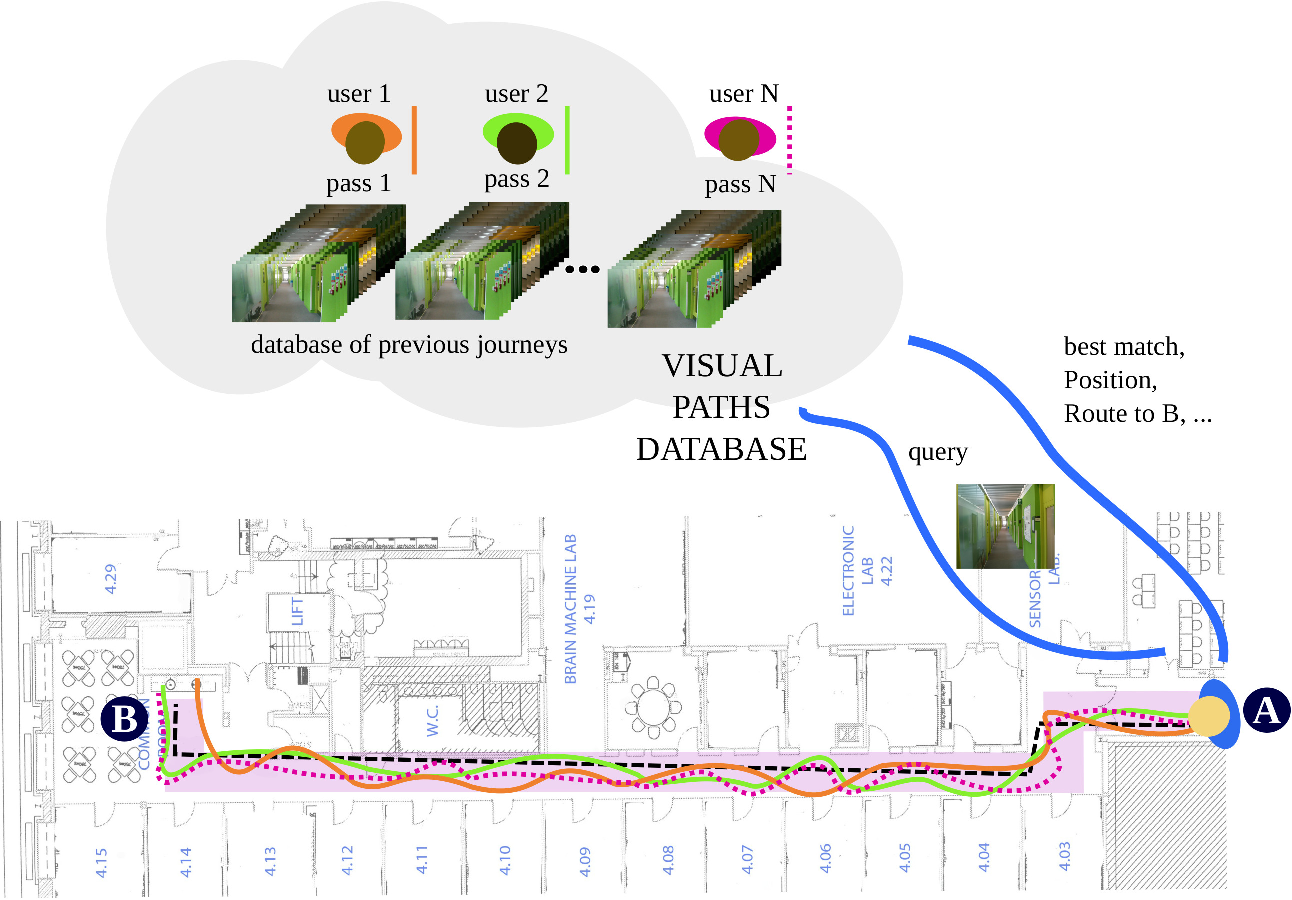
\includegraphics[width=\linewidth]{./gfx/Chapter04/corridor.pdf}
\caption{ A sample path (Corridor 1, C1, from Figure \ref{fig:map_and_legend}) illustrating the multiple passes through the same space. Each of these passes represents a sequence that is either stored in a database, or represents the queries that are submitted against previous journeys. In the assistive context, the user at point A could be a blind or partially sighted user, and he or she would benefit from solutions to the association problem of a query journey relative to previous ``journey experiences'' along roughly the same path, crowdsourced by $N$ users that may be sighted.}
\label{fig:visualpaths}
\end{center}
\end{figure}

\begin{figure}[t]
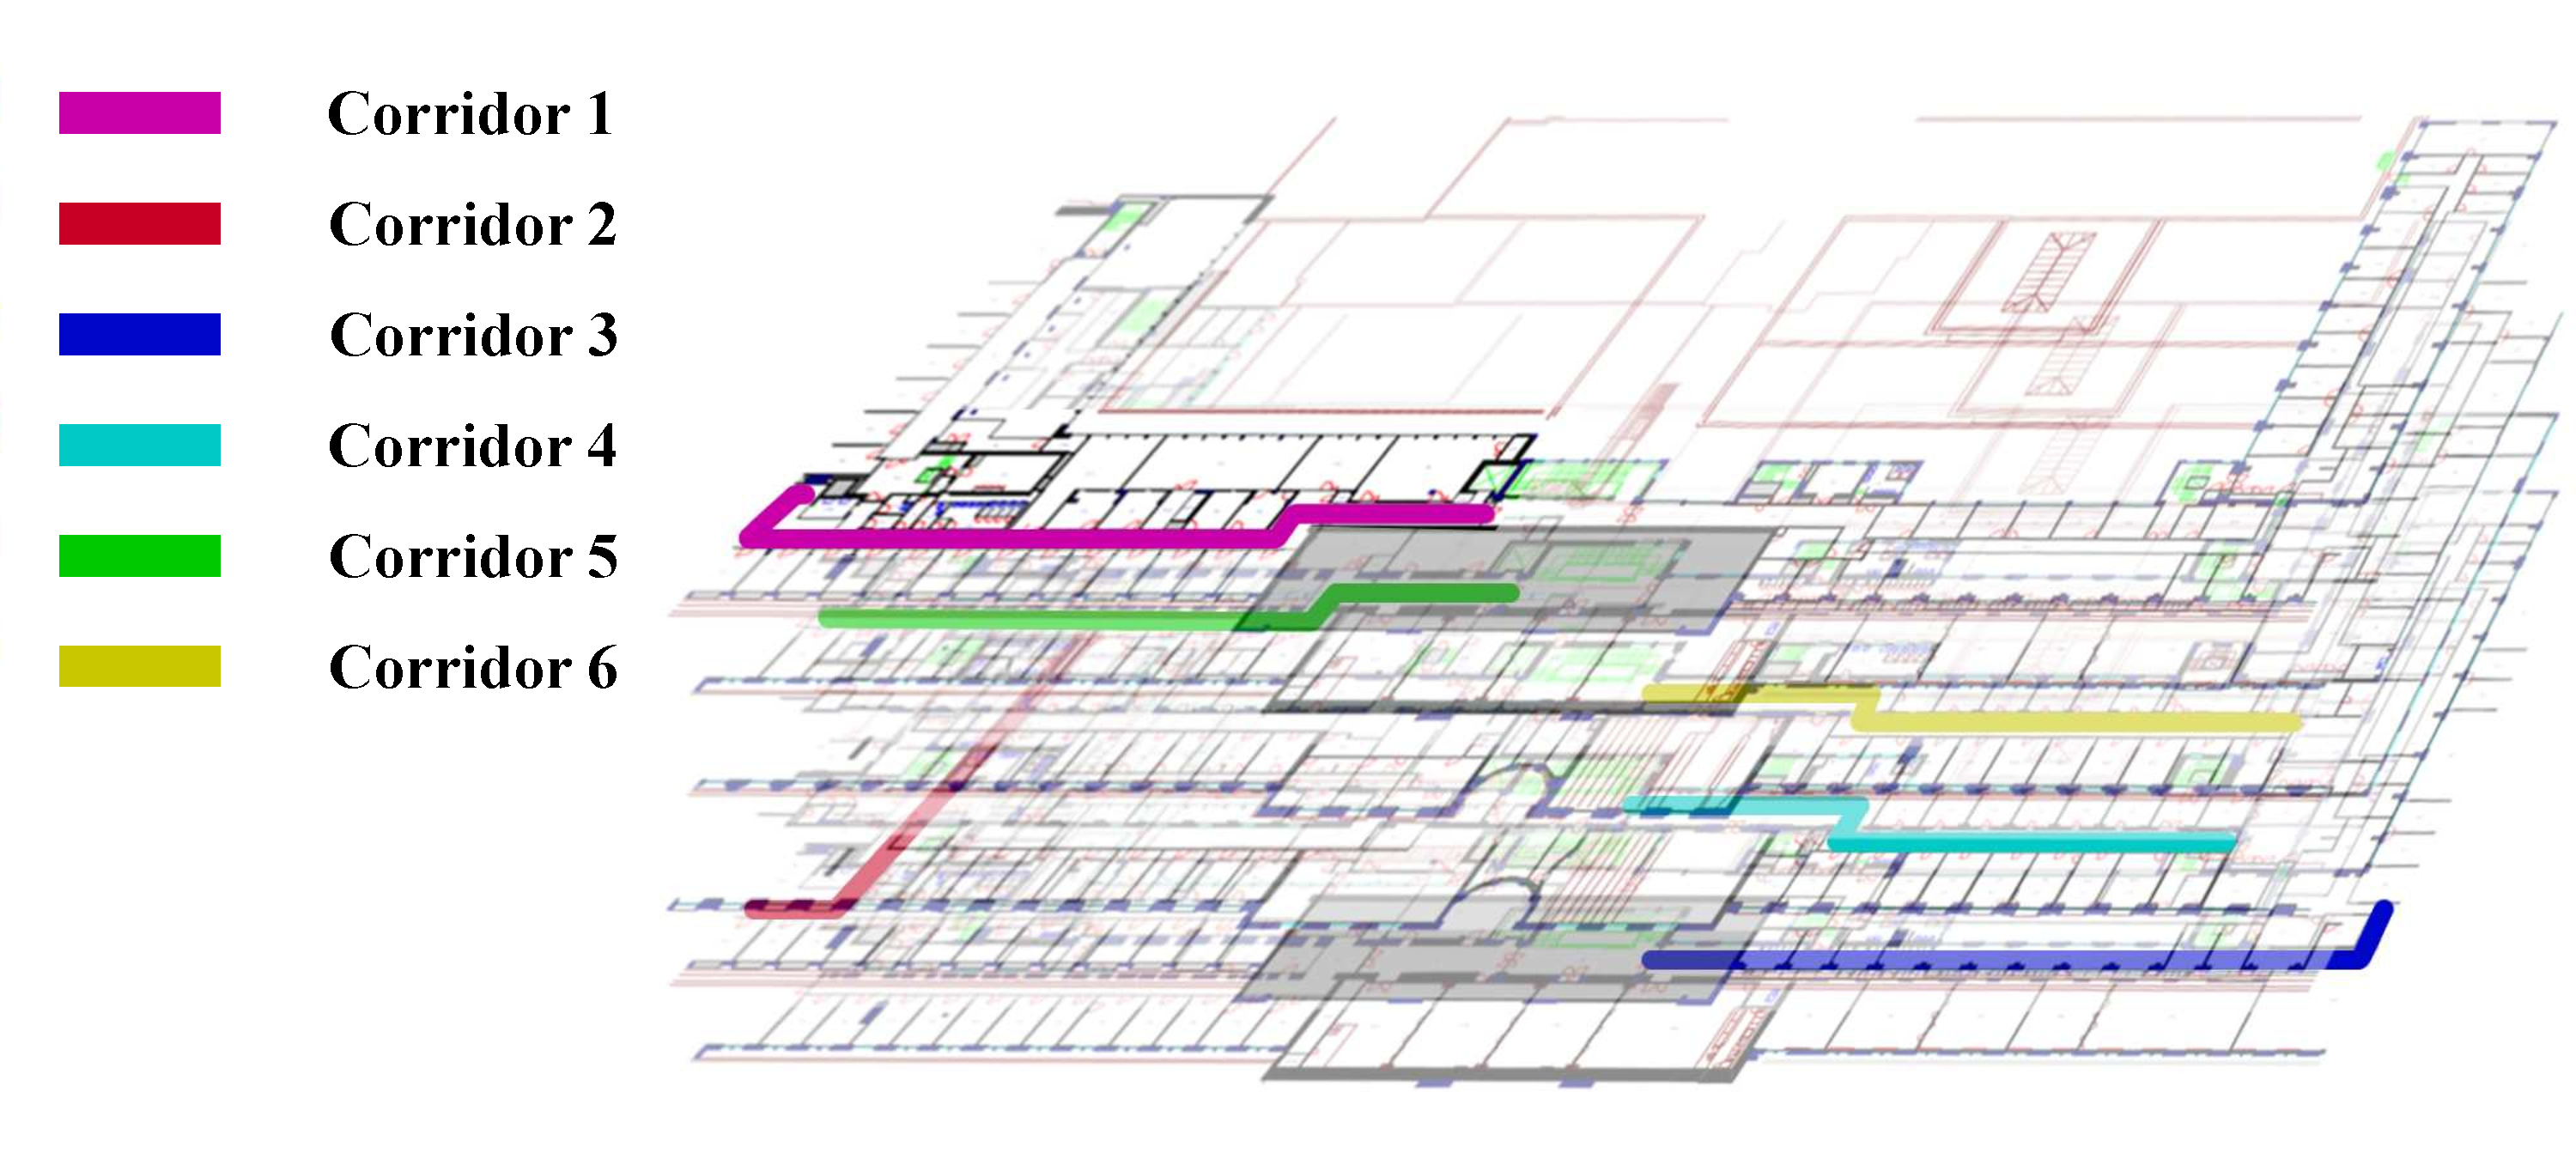
\includegraphics[width=\linewidth]{./gfx/Chapter04/map_and_legend.pdf}\label{fig:visualpathsA}
\caption{Maps of the recording locations.}
\label{fig:map_and_legend}
\end{figure}

\subsection{Alternative methods: non feature-based and sensor merging} 

Fran\c{c}ois Chaumette's team has  recently explored navigation solutions that do not require geometrical nor pixel intensities' features but use mutual information (MI) as a similarity measure. Their system performs a maximisation of the MI that is directly connected with the motion of the robot. These results, and others that rely on tracking visual features \cite{Se2002} cannot serve as a comparison for the current methods either, as they would hinder the fair evaluation of the visual features in isolation.

For outdoor navigation, the Global Positioning System (GPS) has been in widespread use for many years.  In an \textit{indoor} context, localisation technology is still rapidly evolving~\cite{Shen,Wang2012,Quigley2010}.  Using visual information is towards the higher end of computational complexity, and possibly the lower-end of reliability; therefore one would certainly seek to support this approach with other forms of sensor such as received signal strength indication (RSSI) data, magnetometers, and tracking algorithms~\cite{Schroth2011,Schroth2012,Quigley2010}.  In the work presented in this thesis, we seek to explore efficient techniques that could be used to index and compare the visual path information gathered by multiple user journeys, and to measure the potential of vision on its own as a localisation mechanism. 
%

\subsection{Structure from motion (SfM)}

One outcome of the proliferation of digital cameras is the development of structure from motion (SfM) algorithms that can infer 3D models of cities \citep{agarwal2011building} by means of photographs taken by visitors to popular city landmarks. With such images acquired from the internet \citep{snavely2006photo}, bundle adjustment can be used to reconstruct the 3D information about buildings in within well-photographed locations, in addition to the camera pose of every photograph. Similarly to our work, Hile and colleagues also crowdsource location information \citep{hile2010visual}. However, they provide this information through geotagged images from Flickr, to then use Snavely's SfM algorithm \citep{snavely2006photo} to perform camera pose estimation. Using models of a scene constructed using bundle adjustment, the position and pose of a camera from a sequence of new photographs taken from a mobile device can be used as a source of ``visual'' navigation information \citep{ventura2014global}.  However, bundle adjustment is an iterative error minimisation algorithm, and its computational load is still large for real-time use at scale.  Furthermore, it is not entirely clear how the geometric information that is acquired from such models could be updated as aspects of a scene change.


\subsection{Simultaneous localisation and mapping (SLAM)}

Another important branch of vision-based navigation research can be found in robotics. Visual SLAM \citep{konolige2007frame,engelhard2011real,neira2008guest} provides a real time reconstruction of the scene by using stereo cameras (stereoSLAM) or a single one (monoSLAM). Though SLAM is often described for its ability to infer the geometric model of a scene, it also estimates the camera trajectory as part of the camera pose inference. The combination of the two is a powerful source of navigation information. In addition, in subsequent journeys along the same route, geometric information can be refined and also used for refinement of camera pose estimates.

Apart from the possible computational load issues that solutions growing in complexity can entail, the main challenge of SLAM, or the ``SLAM problem'' is to produce an accurate map and therefore a precise localisation. Traditionally, this problem has been studied from two different perspectives: from the image processing and recognition perspective (the latest developments including deep learning approaches \citep{chen2014convolutional}); from a tracking point of view, relying on technologies ranging from depth and inertial sensors to wireless networking to minimise the error drift in the location estimations.

%We are more interested in the first perspective, as we believe our methods presented here can be complementary to SLAM and provide a better location inference acting not only as a loop closure method \citep{glover2012openfabmap} but also as a semantic information retrieval system. 

\citeauthor{davison2007monoslam}~\cite{davison2007monoslam} developed a seminal real time mono SLAM method that used a lightweight Harris feature detector of interesting points within the point of view of the camera. In the next step the system would locate the same feature in a neighbouring patch. Montiel and colleagues, as we will see in the comparison with EKF SLAM of Section~\ref{sec:slamcomp}, took the same monoSLAM approach but aiming for its simplification in degrees of freedom and trying to overcome the problem of the initialisation of features. In \citep{montiel2006unified} they devised an inverse depth parametrisation for point features with 3 degrees of freedom (DOF) instead of the expensive 6.

The complexity of the visual features used for SLAM increased with the introduction of SIFT instead of Harris detectors in \citep{chen2007sift} and \citep{suzuki2011development} to Montiel and Davison's approaches. This opened SLAM to outdoor and more challenging applications as SIFT invariances increased the robustness of the SLAM.

This robustness is key, as some visual SLAM algorithms provide a navigation method suitable for use by autonomous robots \citep{konolige2007frame} but relying on static features from the scene that are subsequently matched before the trajectory is estimated. However, in real life conditions, many of these features are dynamic, since they belong to objects or elements of the scene that are moving (e.g. a crowded scene). Additionally, SLAM algorithms, particularly visual monoSLAM, rely on optic flow induced by ego-motion in order to infer a geometry and build up a map. In the presence of significant additional motion within the scene, algorithms can begin to fail.  One such failure mode is called scale drift and has been studied and taken into account by \cite{strasdat2010scale}. 

Recent vision-based approaches have been developed by Alcantarilla et al. (\cite{alcantarilla2010visual}; \cite{alcantarilla2012combining}) They incorporate dense optical flow estimation into visual SLAM in order to improve the performance of algorithms in crowded and dynamic environments by detecting the presence of objects that are moving relative to the world coordinate system. Additionally, they have developed a fast vision-based method to speed-up the association between visual features and points in large 3D databases \citep{alcantarilla2010learning}. This approach consists of learning the visibility of the features in order to narrow down the number of matching point correspondence candidates.

One of the most recent SLAM algorithms is LSD-SLAM~\citep{engel14eccv}. This semi-dense tracking and mapping method seems to perform well in an indoor SLAM setting. This approach, instead of keypoints and descriptors, uses semi-dense depth maps for tracking by direct image alignment. This is a remarkable step forward, as the semi-dense maps allow lighter frame to frame comparisons, to the point where odometry can be performed on a modern smartphone \citep{schoeps14ismar}. This system, as most SLAM methods, relies greatly on a very accurate camera calibration and initialisation routine, and as we will see in the detailed comparison of Section~\ref{sec:slamcomp}, best results are often achieved under specific conditions, such as monochrome global shutter cameras with fish eye lenses.

\subsection{A biological intuition}

Another source of motivation for the idea of retrieval-based localisation is supported by the well-characterised biological hippocampal place cells~\cite{burgess2002human} that recognise a location from sensory inputs that include those captured by an animal's eyes. This does  \textit{not} suggest that techniques based on optical flow are not relevant: rather, the striking conclusion from recent research is that multiple approaches to visual location inference are at work in biological systems, including optic flow~\cite{Layton2014}, and other mechanisms that may not explicitly involve brain areas specialised in visual motion computation~\cite{hartley2014space}. I will link the findings of the present chapter with this biological intuition in Chapter \ref{ch:chapter5}, where I will propose a model of the hippocampal place cells for indoor localisation.


%------------------------------------------------------------------------- 
\section{Methods}
\label{sec:methods}

In this section I describe the different image description modalities that were evaluated, starting by the feature extraction process, followed by the descriptor quantisation and distance metric used.

\subsection{Pipeline}

I evaluated the performance of several approaches to matching image queries taken from one visual path against the remainder of the visual paths.  In order to index and query the visual path datasets, the sequence of processes that is illustrated in Figure \ref{fig:FigPipeline} was adopted. The details behind each of the processes (e.g. gradient estimation, spatial pooling) are presented in Section \ref{sec:descriptors}.  Both descriptors that operate on \textit{single} frames (spatial) and descriptors that operate on \textit{multiple} frames (spatio-temporal) were compared.

\begin{figure}
\begin{center}
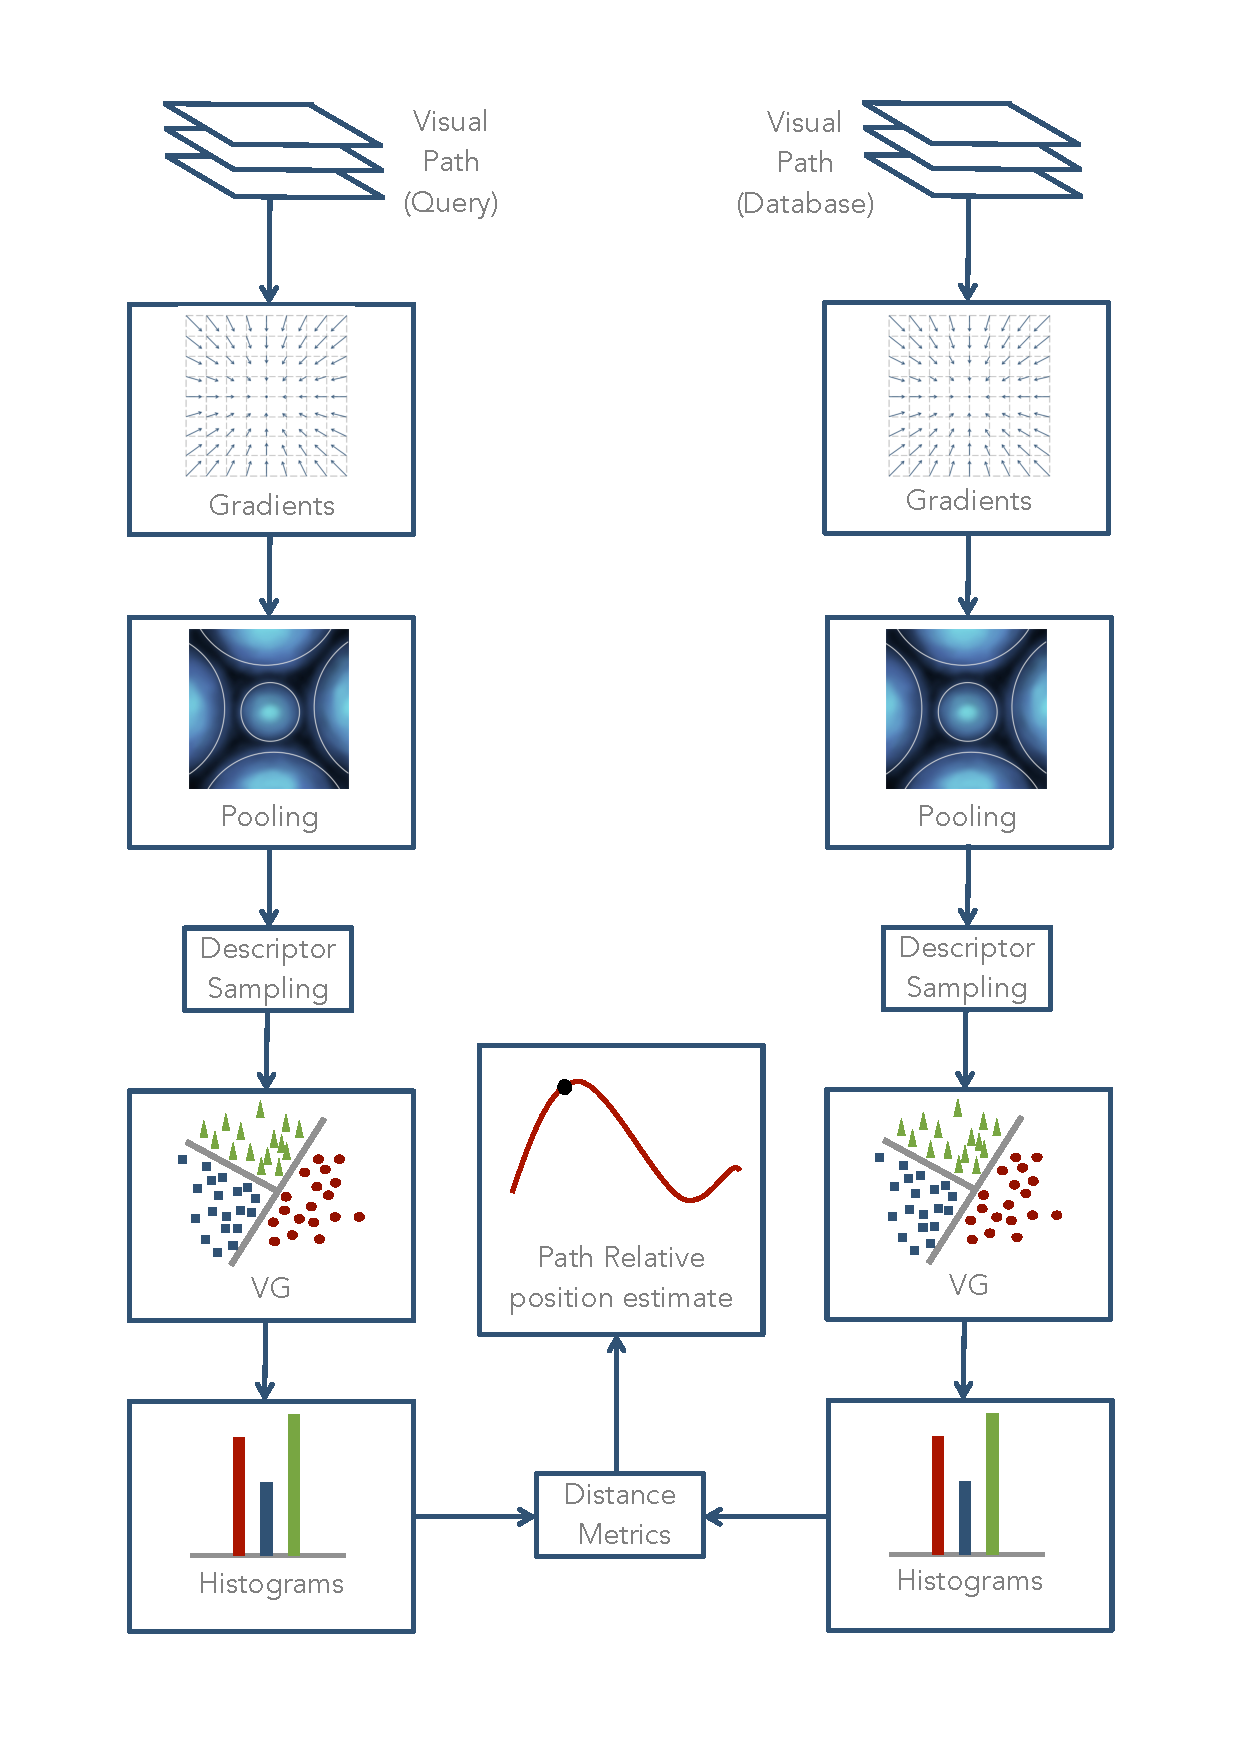
\includegraphics[width=\textwidth]{./gfx/Chapter04/pipeline.pdf}
\caption{The stages in processing image sequences from database and query visual paths are illustrated above.  This does not show the process behind the estimation of ground truth for the experiments, which is described separately in Section \ref{sec:exp_methods}.  Variants of the gradient and pooling operators, quantisation approaches and distance metrics are described in Section \ref{sec:methods}.}
\label{fig:FigPipeline}
\end{center}
\end{figure}

\subsection{Frame-level descriptor}

Inspired by the use of optical flow in motion estimation~\citep{Weickert2006} and space-time descriptors in action recognition \citep{Wang2009} I estimated in-plane motion vectors using a simple approach.  Derivative filters were applied along $(x,y,t)$ dimensions, yielding a 2D$+t$, i.e. spatio-temporal, gradient field.  To capture variations in chromatic content from the visual sequence, spatio-temporal gradients were computed separately for each of the three RGB channels of the pre-processed video sequences.  This yielded a $3\times 3$ matrix at each point in space, effectively a \textit{chromatic Jacobian} (Eq.~\ref{eq:CJ}).  

\begin{equation}
\mathbf{J} = \left (
\begin{array}{ccc}
\frac{\partial I_r}{\partial_x} & \frac{\partial I_r}{\partial_y}   & \frac{\partial I_r}{\partial_t} \\
\frac{\partial I_g}{\partial_x}   & \frac{\partial I_g}{\partial_y}  &  \frac{\partial I_g}{\partial_t} \\
\frac{\partial I_b}{\partial_x}  & \frac{\partial  I_b}{\partial_y}  &  \frac{\partial I_b}{\partial_t} 
\end{array} 
\right )
\label{eq:CJ}
\end{equation}

Temporal smoothing was applied along the time dimension, with a support of 11 neighbouring frames. Finally, the components of the matrix were each averaged (pooled) over 16 distinct spatial regions (see Figure~\ref{fig:pooling4lwcolor}), not very dissimilar to those to be described later in this thesis. 



\begin{figure}[h!]
\centering
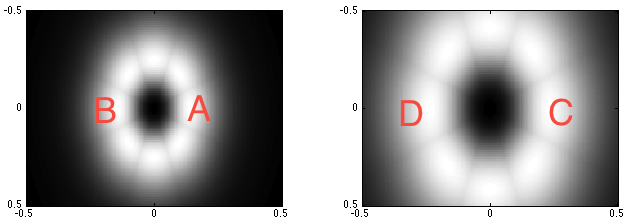
\includegraphics[width=\linewidth]{./gfx/Chapter04/pooling_lwcolor.png}
\caption{A maximum projection intensity rendering of 16 pooling regions over space. The $x$ components of descriptor component time series from regions $A$, $B$, $C$ and $D$ are shown in Figure~\ref{fig:Traces}.}
\label{fig:pooling4lwcolor}
\end{figure}


The rationale is that ego-motion is likely to be an important visual cue in human pedestrian navigation, particularly in close or cluttered spaces. Rather than explicit computation of optical flow, the collection of gradient information over different pooling regions of space captures and encodes relevant motion in the form of time series.  The 16 proposed pooling regions illustrated in Figure \ref{fig:pooling4lwcolor} were selected to capture elements of the chromatic space-time Jacobian within two sectors at different radii from the centre of the frame (e.g. A and C, and B and D); to capture information in pairs of regions (such as A and B) that are diametrically opposed from each other horizontally, and also vertically.  Diagonal regions were also proposed, yielding fairly uniform angular coverage over image space. Spatial and temporal gradients in the centre of the frame were not encoded because this region contains less visible motion over equivalent time scales to the more peripheral regions.  


For each visual path, this yielded a total of $16\times 9 = 144$ separate time-series, or signals, of length approximately equal to the video sequences.  An illustration of the time series for one visual path is shown in Figure~\ref{fig:Traces}. Effectively, for each frame, a 144-dimensional descriptor is captured. The elements of this descriptor describe the weighted average of the Jacobian elements within the respective pooling regions that can be used for indexing and matching visual path locations.

\begin{figure}
\begin{center}
	\setlength\figureheight{0.5\linewidth}
	\setlength\figurewidth{0.9\linewidth}
		% This file was created by matlab2tikz.
% Minimal pgfplots version: 1.3
%
%The latest updates can be retrieved from
%  http://www.mathworks.com/matlabcentral/fileexchange/22022-matlab2tikz
%where you can also make suggestions and rate matlab2tikz.
%
\definecolor{mycolor1}{rgb}{0.00000,0.49804,0.00000}%
%
\begin{tikzpicture}

\begin{axis}[%
width=0.95092\figurewidth,
height=\figureheight,
at={(0\figurewidth,0\figureheight)},
scale only axis,
xmin=0,
xmax=2000,
xlabel={Frame ID},
ymin=-1.5,
ymax=1.5,
ylabel={Lobe Outputs},
/pgf/number format/1000 sep={}
]
\addplot [color=black!20!red,solid,line width=3.0pt,forget plot]
  table[row sep=crcr]{%
1	0.478423475810152\\
2	0.479366908471821\\
3	0.481229169293418\\
4	0.482766095513316\\
5	0.480457324574169\\
6	0.471532766626857\\
7	0.467135278955816\\
8	0.465319203026626\\
9	0.465126659860796\\
10	0.46441075998703\\
11	0.461172115635224\\
12	0.454984753044735\\
13	0.446897492466023\\
14	0.440316024235594\\
15	0.433030385972121\\
16	0.424551721133589\\
17	0.415353563443456\\
18	0.405986716143052\\
19	0.396025498610686\\
20	0.385021234077294\\
21	0.373256353583084\\
22	0.360698392874367\\
23	0.349140894769336\\
24	0.33780696005398\\
25	0.325996447747139\\
26	0.31418262614635\\
27	0.302408693806229\\
28	0.291398306815973\\
29	0.281007838509357\\
30	0.269953978610163\\
31	0.258752427561295\\
32	0.246891949533784\\
33	0.235407247029794\\
34	0.224454632329207\\
35	0.214140323676815\\
36	0.205239640202436\\
37	0.197977871098073\\
38	0.191528073186217\\
39	0.18635791052726\\
40	0.182581676383847\\
41	0.181529468198483\\
42	0.182947602486377\\
43	0.185198504755744\\
44	0.188304943380743\\
45	0.192878273398197\\
46	0.199125719834894\\
47	0.207878995767175\\
48	0.218875824694265\\
49	0.231687311384122\\
50	0.244329980480234\\
51	0.256973685862441\\
52	0.270600391678147\\
53	0.28598399703983\\
54	0.302245525147571\\
55	0.319994068755042\\
56	0.33917308309296\\
57	0.359988994806679\\
58	0.381107977837565\\
59	0.402115142186688\\
60	0.423411713747468\\
61	0.444360566601079\\
62	0.464934007059671\\
63	0.48520964068844\\
64	0.505521836867187\\
65	0.524811726668574\\
66	0.542589481772491\\
67	0.55791846500364\\
68	0.571835080792125\\
69	0.58504178813612\\
70	0.597204454985717\\
71	0.60843391041389\\
72	0.619312228629623\\
73	0.62803030011947\\
74	0.632174986861623\\
75	0.63486670088825\\
76	0.637463527322466\\
77	0.639285678328232\\
78	0.639431927294954\\
79	0.638131660227779\\
80	0.635784152536763\\
81	0.632226207788491\\
82	0.627691467840153\\
83	0.624290517693087\\
84	0.620195472703703\\
85	0.614787203581477\\
86	0.607785525061724\\
87	0.600223384976833\\
88	0.591190098559401\\
89	0.58002516452415\\
90	0.569427781852709\\
91	0.560178164579814\\
92	0.551708349106014\\
93	0.543511224518442\\
94	0.535535783747178\\
95	0.528643607011768\\
96	0.521730918226053\\
97	0.512912314504612\\
98	0.50480283848574\\
99	0.500737673757958\\
100	0.499155872786664\\
101	0.49823385538912\\
102	0.498243590015213\\
103	0.499332874520063\\
104	0.502607054181558\\
105	0.507030261474608\\
106	0.513042364936008\\
107	0.520103201906619\\
108	0.525062955291585\\
109	0.530509965401758\\
110	0.537841665534304\\
111	0.548803916782087\\
112	0.56112504293318\\
113	0.575485727720288\\
114	0.591739829322705\\
115	0.607012194299988\\
116	0.620889044400804\\
117	0.635466505601124\\
118	0.650511095225915\\
119	0.665486881301443\\
120	0.679729307559514\\
121	0.695026715930106\\
122	0.711190580778835\\
123	0.727010846933572\\
124	0.741721377083027\\
125	0.755546249394263\\
126	0.767950292783871\\
127	0.77927862188237\\
128	0.788978271362462\\
129	0.797068608814914\\
130	0.80407726167043\\
131	0.809920190950866\\
132	0.815408821909345\\
133	0.82180140504733\\
134	0.828073178483939\\
135	0.833365105552507\\
136	0.835960783254066\\
137	0.836906701607581\\
138	0.836857797117119\\
139	0.835908033891795\\
140	0.834004838378375\\
141	0.830569450253314\\
142	0.825679696959058\\
143	0.821529981872751\\
144	0.818354927372845\\
145	0.815357525742975\\
146	0.811359819810923\\
147	0.807142708116881\\
148	0.802726793098333\\
149	0.798169323316241\\
150	0.794495101083461\\
151	0.792751624345942\\
152	0.791318492005475\\
153	0.789239297723294\\
154	0.786302625051832\\
155	0.78348156793567\\
156	0.780527965518993\\
157	0.7780967929403\\
158	0.777571772883667\\
159	0.779062562210322\\
160	0.781024330890521\\
161	0.783064738679351\\
162	0.785821961726275\\
163	0.789730788781626\\
164	0.795812749129109\\
165	0.803676154956108\\
166	0.813285604468446\\
167	0.823431499990514\\
168	0.832692846657167\\
169	0.841498516002792\\
170	0.850356371013845\\
171	0.859648408992208\\
172	0.869258612895422\\
173	0.878990966348823\\
174	0.888952528211547\\
175	0.898000310526157\\
176	0.905719497009581\\
177	0.912663730532023\\
178	0.919472953988917\\
179	0.925825919878756\\
180	0.931498094416062\\
181	0.936738828208945\\
182	0.940802909738172\\
183	0.942250463921085\\
184	0.942069321137298\\
185	0.941428409944246\\
186	0.940332373056597\\
187	0.938082991434418\\
188	0.934393450967925\\
189	0.928316521056502\\
190	0.920623380774929\\
191	0.911711278523055\\
192	0.902016719951991\\
193	0.892181096622738\\
194	0.881215688391224\\
195	0.869861970185229\\
196	0.858643023200622\\
197	0.848102158553169\\
198	0.838823601474886\\
199	0.830453623156386\\
200	0.823186241205909\\
201	0.816593874603728\\
202	0.810557947708279\\
203	0.805413641583299\\
204	0.80176722331086\\
205	0.799181875819563\\
206	0.79738365975945\\
207	0.796664406858947\\
208	0.797138518163165\\
209	0.797546444938644\\
210	0.798281427792511\\
211	0.800406974752463\\
212	0.803366425816269\\
213	0.806928670393699\\
214	0.812095744940922\\
215	0.818513154856185\\
216	0.826195478520739\\
217	0.834747721267386\\
218	0.84334956155586\\
219	0.852643506720833\\
220	0.862567847983302\\
221	0.872308093729733\\
222	0.881589934565189\\
223	0.889148408448975\\
224	0.896960659852746\\
225	0.903995530394563\\
226	0.910281625614084\\
227	0.916132607496594\\
228	0.921210403489302\\
229	0.924667954075016\\
230	0.927637237163092\\
231	0.929992990961063\\
232	0.930809032070742\\
233	0.930558734928728\\
234	0.931099061627066\\
235	0.931780216398459\\
236	0.931934611131403\\
237	0.932089476820044\\
238	0.931877431062372\\
239	0.931442651483296\\
240	0.931766182689758\\
241	0.932103030561222\\
242	0.931541746955839\\
243	0.931215333869377\\
244	0.931234210639633\\
245	0.930941092601123\\
246	0.930520240215581\\
247	0.929846476499539\\
248	0.929161737850514\\
249	0.926955348621798\\
250	0.924184384756682\\
251	0.921529057790599\\
252	0.918348857239742\\
253	0.915254418017943\\
254	0.91231595488496\\
255	0.908574718778251\\
256	0.905233131600425\\
257	0.900756496595092\\
258	0.89658843714997\\
259	0.892620858089825\\
260	0.888288024042486\\
261	0.882992729342823\\
262	0.876887629792596\\
263	0.869947460083265\\
264	0.861595128702909\\
265	0.853057308974447\\
266	0.845286791125013\\
267	0.838051772325074\\
268	0.828950132845458\\
269	0.817905736829549\\
270	0.80737752739851\\
271	0.797749659983441\\
272	0.789082083634466\\
273	0.780783647768676\\
274	0.773075228543489\\
275	0.766492591847616\\
276	0.760130260977703\\
277	0.754089758346544\\
278	0.749000924213154\\
279	0.744833987079076\\
280	0.741789918143742\\
281	0.738295396322645\\
282	0.736139512725019\\
283	0.734527494982358\\
284	0.732930734975432\\
285	0.731311251145296\\
286	0.730696845568487\\
287	0.731590603303687\\
288	0.733726160618596\\
289	0.737245577106665\\
290	0.740611010281645\\
291	0.742697014745359\\
292	0.745012324750688\\
293	0.749231736977607\\
294	0.754950136129541\\
295	0.759924636650433\\
296	0.763797834009338\\
297	0.766974029123943\\
298	0.770220779239298\\
299	0.773035591725566\\
300	0.774966718357232\\
301	0.776449118135486\\
302	0.778073781368988\\
303	0.778923007902361\\
304	0.778322923376755\\
305	0.776610193627003\\
306	0.774178885687438\\
307	0.770863462277611\\
308	0.766188495034984\\
309	0.760650573019204\\
310	0.75459241132339\\
311	0.748615658353467\\
312	0.740835852181728\\
313	0.731155893415984\\
314	0.719497520493359\\
315	0.706996220701413\\
316	0.697230382800844\\
317	0.688993060913317\\
318	0.680178662354028\\
319	0.669724851311292\\
320	0.658806500974434\\
321	0.648401988090271\\
322	0.63747663284657\\
323	0.626580332744944\\
324	0.615969109162369\\
325	0.60529639224821\\
326	0.594200998484088\\
327	0.583204374663616\\
328	0.573693164757661\\
329	0.566492385688038\\
330	0.560737955373381\\
331	0.555790088059085\\
332	0.550814438921867\\
333	0.547557651791943\\
334	0.545087391407087\\
335	0.544438445775666\\
336	0.545256744741098\\
337	0.548093401150017\\
338	0.553428805578565\\
339	0.561285404602064\\
340	0.569795738759842\\
341	0.575357296155008\\
342	0.580348136819029\\
343	0.586324651234166\\
344	0.594409920935724\\
345	0.60296602796028\\
346	0.610213631711131\\
347	0.618419262112479\\
348	0.62686461667112\\
349	0.63517386063126\\
350	0.642466340628285\\
351	0.651134391457007\\
352	0.65958982310136\\
353	0.665442859827803\\
354	0.669306890998425\\
355	0.67080192821835\\
356	0.670971089842836\\
357	0.671721999047918\\
358	0.670668043155948\\
359	0.667577232957434\\
360	0.661736770633546\\
361	0.652310252392444\\
362	0.640314204614199\\
363	0.62934499264667\\
364	0.620923818564774\\
365	0.613743524239687\\
366	0.606058359359325\\
367	0.595916735160531\\
368	0.584310029106154\\
369	0.572795112065077\\
370	0.562056767993993\\
371	0.552771613318018\\
372	0.543099589495372\\
373	0.533589557290018\\
374	0.524468673342719\\
375	0.516662291387272\\
376	0.509369105172764\\
377	0.503092881445212\\
378	0.498497876495193\\
379	0.494156688578165\\
380	0.4892953446084\\
381	0.486690758716152\\
382	0.486951093489154\\
383	0.487871090706115\\
384	0.489646254941659\\
385	0.493575268655508\\
386	0.501842169894304\\
387	0.512691931549127\\
388	0.52233173913238\\
389	0.529350271542563\\
390	0.534131708305495\\
391	0.53945515578787\\
392	0.547149092485163\\
393	0.556074578668626\\
394	0.565367845448869\\
395	0.574563851770594\\
396	0.58369120680637\\
397	0.592354452804663\\
398	0.599255068801658\\
399	0.60510666163172\\
400	0.609993610068132\\
401	0.613584331289871\\
402	0.6171064548318\\
403	0.620472058007831\\
404	0.624394006135968\\
405	0.630407654692023\\
406	0.634515054792211\\
407	0.636171824753249\\
408	0.638257389570279\\
409	0.641022823461059\\
410	0.641290958406636\\
411	0.637682803141334\\
412	0.63296842937218\\
413	0.628566535576939\\
414	0.624186518958007\\
415	0.620839023581083\\
416	0.61736325083783\\
417	0.612232685564848\\
418	0.606004604352032\\
419	0.598626294283667\\
420	0.590533090585531\\
421	0.582338806438176\\
422	0.573649167635292\\
423	0.56667590930853\\
424	0.561006013662021\\
425	0.555370354899774\\
426	0.548629867349369\\
427	0.539759107056932\\
428	0.530549458185265\\
429	0.520957074087327\\
430	0.511291311171412\\
431	0.504607145452026\\
432	0.498569276421071\\
433	0.490751634203754\\
434	0.483325550855345\\
435	0.479085405326716\\
436	0.476485616011511\\
437	0.472859438329265\\
438	0.468254690681345\\
439	0.462671942265572\\
440	0.455659030498696\\
441	0.44790569034565\\
442	0.440057555365511\\
443	0.431963538860596\\
444	0.423349688482459\\
445	0.41417353005424\\
446	0.403261695197691\\
447	0.39255640566551\\
448	0.380051819677597\\
449	0.364265452483586\\
450	0.346711495099495\\
451	0.328427404077206\\
452	0.309682822892963\\
453	0.289656515014679\\
454	0.268895148275078\\
455	0.247946968037658\\
456	0.223799185424337\\
457	0.19758939602421\\
458	0.172410659277262\\
459	0.146477756462907\\
460	0.117953893019244\\
461	0.0886742094783798\\
462	0.0599190965050472\\
463	0.0312011068763284\\
464	0.00265463934518837\\
465	-0.0245042985755649\\
466	-0.0501302687206395\\
467	-0.0748399919888027\\
468	-0.0984550446783204\\
469	-0.121430938408861\\
470	-0.143952409688462\\
471	-0.165517003882249\\
472	-0.187030676895488\\
473	-0.206946268637384\\
474	-0.224152137539631\\
475	-0.239334897469086\\
476	-0.253320217422841\\
477	-0.26579960061356\\
478	-0.276938078054406\\
479	-0.287460643190965\\
480	-0.298729385824325\\
481	-0.309088197836501\\
482	-0.318480623017916\\
483	-0.326965456607423\\
484	-0.334912907490685\\
485	-0.341419575281968\\
486	-0.347596246324714\\
487	-0.352837252799339\\
488	-0.358272536172128\\
489	-0.363582328762272\\
490	-0.36875400652113\\
491	-0.37392250151809\\
492	-0.379629826455048\\
493	-0.385371006721815\\
494	-0.391278993155143\\
495	-0.397531836532589\\
496	-0.403600910712008\\
497	-0.409234677229329\\
498	-0.414567884662683\\
499	-0.420227099696831\\
500	-0.425989088083901\\
501	-0.430286500332786\\
502	-0.432558440993527\\
503	-0.434777293030962\\
504	-0.438621302028341\\
505	-0.44152673662196\\
506	-0.442399613598232\\
507	-0.441379106561424\\
508	-0.439423898273263\\
509	-0.437308088114248\\
510	-0.435835049315003\\
511	-0.43455697913992\\
512	-0.433308763569472\\
513	-0.431263653251666\\
514	-0.428216713639013\\
515	-0.42456499597171\\
516	-0.420278698139338\\
517	-0.415438373406831\\
518	-0.409743490313308\\
519	-0.40233239515326\\
520	-0.393147168443025\\
521	-0.383184580098384\\
522	-0.372876143638481\\
523	-0.362077749143372\\
524	-0.35001412963122\\
525	-0.335890815698716\\
526	-0.32017919419983\\
527	-0.302970502432522\\
528	-0.283780356942662\\
529	-0.260102627190799\\
530	-0.235026577519455\\
531	-0.210130951660579\\
532	-0.185825381250557\\
533	-0.160857604993625\\
534	-0.135733631604021\\
535	-0.109537731386093\\
536	-0.0826464430904808\\
537	-0.0559008808260719\\
538	-0.0296620303603774\\
539	-0.0057280618576837\\
540	0.0159161158513026\\
541	0.0358234139072528\\
542	0.0553760230680909\\
543	0.0743524684125142\\
544	0.0918764101327688\\
545	0.10782952319202\\
546	0.123584518588638\\
547	0.139846319774422\\
548	0.155958466504703\\
549	0.171287142316491\\
550	0.184569852229735\\
551	0.194274025813045\\
552	0.199618131741346\\
553	0.200644611451442\\
554	0.197264991147877\\
555	0.191131980210762\\
556	0.183630139012798\\
557	0.176231243993607\\
558	0.168034379586192\\
559	0.159235485379583\\
560	0.149520885289984\\
561	0.139784423613506\\
562	0.12960745174128\\
563	0.119419184123652\\
564	0.109626432188812\\
565	0.0988652831294145\\
566	0.0880583773473173\\
567	0.0756909788645469\\
568	0.0609599810538846\\
569	0.0450395728193945\\
570	0.0291458375397158\\
571	0.0118925138170751\\
572	-0.00633588753659311\\
573	-0.0257563310752043\\
574	-0.0453002555375864\\
575	-0.0645670619699725\\
576	-0.0825129675568671\\
577	-0.0988108791142853\\
578	-0.112777774203832\\
579	-0.124211903406334\\
580	-0.134477429410876\\
581	-0.145588753468661\\
582	-0.157842150728577\\
583	-0.170897637351807\\
584	-0.183086759186987\\
585	-0.194359116918262\\
586	-0.205272859418493\\
587	-0.215721908249008\\
588	-0.225179013309288\\
589	-0.231920682535171\\
590	-0.232063607416082\\
591	-0.225725861355889\\
592	-0.211791894336703\\
593	-0.196396946073159\\
594	-0.187315022943858\\
595	-0.179659036109633\\
596	-0.172476565754228\\
597	-0.174058357163261\\
598	-0.178472466433826\\
599	-0.182291284845175\\
600	-0.185961854356787\\
601	-0.190784214435554\\
602	-0.19782214471047\\
603	-0.206662103992396\\
604	-0.217140376048845\\
605	-0.228920808789065\\
606	-0.239989234076667\\
607	-0.249271897951022\\
608	-0.257046316495592\\
609	-0.260311755019508\\
610	-0.261094372386751\\
611	-0.261463306050459\\
612	-0.260077432563686\\
613	-0.255259886950185\\
614	-0.249914329015606\\
615	-0.245579484710737\\
616	-0.237511582499471\\
617	-0.224782111331121\\
618	-0.206659501217624\\
619	-0.179269045213163\\
620	-0.147047541169647\\
621	-0.110833348203805\\
622	-0.0644374589442894\\
623	-0.0144230088745727\\
624	0.0349569731736181\\
625	0.0836809252809201\\
626	0.132231123572113\\
627	0.182039542051231\\
628	0.232865927274984\\
629	0.283837301890995\\
630	0.335359083766638\\
631	0.385570008463858\\
632	0.43286937953223\\
633	0.478245560486183\\
634	0.517864030930993\\
635	0.553791876995239\\
636	0.588400520992989\\
637	0.620819630590569\\
638	0.646945301614947\\
639	0.669654548311357\\
640	0.688214373915104\\
641	0.696573049426446\\
642	0.693751968755102\\
643	0.685925066273629\\
644	0.674945388896997\\
645	0.659285928154768\\
646	0.638420439313938\\
647	0.612253583781938\\
648	0.581055659941831\\
649	0.544227141045701\\
650	0.504678374224367\\
651	0.46343869882207\\
652	0.419239869967945\\
653	0.372620818913237\\
654	0.323502178313398\\
655	0.273517778450754\\
656	0.223716205601337\\
657	0.174117671829293\\
658	0.123261873411656\\
659	0.0723767348174313\\
660	0.0225220769796427\\
661	-0.0273057535716438\\
662	-0.0775566496792226\\
663	-0.126811774493291\\
664	-0.175115938498014\\
665	-0.221445357751668\\
666	-0.26579478966464\\
667	-0.309281284112579\\
668	-0.352636229741457\\
669	-0.395477501324076\\
670	-0.437452445048717\\
671	-0.476575738180182\\
672	-0.511123866473619\\
673	-0.540927960351397\\
674	-0.564727743311842\\
675	-0.584086622431623\\
676	-0.600959515955009\\
677	-0.616895201030977\\
678	-0.630592636509394\\
679	-0.639548411147805\\
680	-0.6454701705845\\
681	-0.650076172511113\\
682	-0.654063344988193\\
683	-0.656836907966737\\
684	-0.659058835000752\\
685	-0.66184977244245\\
686	-0.664428843168314\\
687	-0.666422616340566\\
688	-0.667234243658665\\
689	-0.667506098604981\\
690	-0.668064675752404\\
691	-0.668406500987405\\
692	-0.668124857255576\\
693	-0.66786308144935\\
694	-0.66522425178749\\
695	-0.659924292537036\\
696	-0.653286544968175\\
697	-0.646554059581641\\
698	-0.639632270608876\\
699	-0.632013900358876\\
700	-0.624478823442842\\
701	-0.618486062398423\\
702	-0.610062488783262\\
703	-0.598975373306764\\
704	-0.587623860624313\\
705	-0.57778624443021\\
706	-0.568339783048839\\
707	-0.557589203127987\\
708	-0.545151768384314\\
709	-0.532349297964714\\
710	-0.518588156488781\\
711	-0.50365488265783\\
712	-0.487386727691417\\
713	-0.46960199292097\\
714	-0.450642176311294\\
715	-0.429878673313613\\
716	-0.407628899055126\\
717	-0.383266755537444\\
718	-0.357178156861041\\
719	-0.331429235516075\\
720	-0.305980699941064\\
721	-0.282125135520347\\
722	-0.258616970950754\\
723	-0.235374662563603\\
724	-0.213545232792778\\
725	-0.192660750472294\\
726	-0.170042105971684\\
727	-0.147457157055794\\
728	-0.126728469187061\\
729	-0.10739269493753\\
730	-0.0878418893646672\\
731	-0.0676235958588538\\
732	-0.0479821214980763\\
733	-0.0300860326899227\\
734	-0.0129479401205941\\
735	0.0032210342542986\\
736	0.0186306866023571\\
737	0.032653133514942\\
738	0.0445614125150381\\
739	0.0546225076695113\\
740	0.0614693933463363\\
741	0.0652173301710767\\
742	0.065302330938441\\
743	0.0637687306907422\\
744	0.0609737778157134\\
745	0.0556958951972739\\
746	0.0503300685279909\\
747	0.0445363726835402\\
748	0.0383721904673766\\
749	0.0322586078512957\\
750	0.0258949642237177\\
751	0.0204678429346564\\
752	0.0159559663429263\\
753	0.0111657803171418\\
754	0.00506706126658513\\
755	-0.000592743387759092\\
756	-0.0067245545252524\\
757	-0.0131606140136833\\
758	-0.0189652297149806\\
759	-0.0243550358000096\\
760	-0.0296683443676077\\
761	-0.0359389936958263\\
762	-0.0415010459130968\\
763	-0.0461020555599898\\
764	-0.0503745563570791\\
765	-0.0547536203083109\\
766	-0.0598200113468027\\
767	-0.0635652859185414\\
768	-0.0664923127182155\\
769	-0.0688422140399925\\
770	-0.0708572206269417\\
771	-0.0735825732689341\\
772	-0.0760900110063039\\
773	-0.0787741634869906\\
774	-0.0815220530230071\\
775	-0.0849365776808986\\
776	-0.0895430257787376\\
777	-0.0950969318008738\\
778	-0.101038943998672\\
779	-0.106504305381012\\
780	-0.112241125381249\\
781	-0.118235643280557\\
782	-0.123900658317143\\
783	-0.130059119708749\\
784	-0.135931650699571\\
785	-0.140936173922718\\
786	-0.145412593091228\\
787	-0.150394560038771\\
788	-0.155427010047929\\
789	-0.160219446168533\\
790	-0.164017345296247\\
791	-0.166965913641971\\
792	-0.17020613017607\\
793	-0.174660493344948\\
794	-0.179122626557963\\
795	-0.182604262105637\\
796	-0.185334716111877\\
797	-0.188545307410717\\
798	-0.191747722592882\\
799	-0.19442263281418\\
800	-0.196468118165237\\
801	-0.19812031851199\\
802	-0.19946813444028\\
803	-0.19998924792885\\
804	-0.200105255186586\\
805	-0.199912853990973\\
806	-0.199291194511334\\
807	-0.198381056251999\\
808	-0.197368745446036\\
809	-0.196248932271437\\
810	-0.19627155742973\\
811	-0.196111617773211\\
812	-0.19636057224655\\
813	-0.197069274471812\\
814	-0.197950283806734\\
815	-0.198831455090874\\
816	-0.199995856179882\\
817	-0.202155914827573\\
818	-0.204047644492199\\
819	-0.206397221470894\\
820	-0.208949076316586\\
821	-0.211090882470655\\
822	-0.213421897963965\\
823	-0.215334292549716\\
824	-0.217166081045458\\
825	-0.218616020689051\\
826	-0.219746612452523\\
827	-0.221244685081512\\
828	-0.222785026817637\\
829	-0.224476593351327\\
830	-0.225991725257097\\
831	-0.227977425334735\\
832	-0.229971814066493\\
833	-0.232194782535\\
834	-0.23538236770433\\
835	-0.238443181432362\\
836	-0.242149862292199\\
837	-0.24538405964362\\
838	-0.248827967385692\\
839	-0.252623783149068\\
840	-0.256424244667313\\
841	-0.260583408463343\\
842	-0.264241507854605\\
843	-0.268041298855029\\
844	-0.271081956818793\\
845	-0.273726092348262\\
846	-0.276703755032935\\
847	-0.278999591158994\\
848	-0.281622743834844\\
849	-0.284863603281404\\
850	-0.288569381819529\\
851	-0.292795603582639\\
852	-0.297226098830009\\
853	-0.302268870834714\\
854	-0.307147510535126\\
855	-0.312582169738753\\
856	-0.317773633226067\\
857	-0.323405836091823\\
858	-0.329305279959834\\
859	-0.335124178601211\\
860	-0.33990493718513\\
861	-0.344763267789696\\
862	-0.349507529894172\\
863	-0.353696278158558\\
864	-0.357583290133119\\
865	-0.362080724582487\\
866	-0.365712585479297\\
867	-0.369592849666891\\
868	-0.372698834498422\\
869	-0.376589831425447\\
870	-0.38122065372781\\
871	-0.385858152043355\\
872	-0.390484370539839\\
873	-0.395100352492484\\
874	-0.399400537350651\\
875	-0.402512802406059\\
876	-0.405230583830427\\
877	-0.407075000266335\\
878	-0.408889607220129\\
879	-0.409830855612531\\
880	-0.410196718197178\\
881	-0.409732003154565\\
882	-0.407421070308391\\
883	-0.404084984586437\\
884	-0.399436256620391\\
885	-0.394615521075921\\
886	-0.388928227271144\\
887	-0.384000902591724\\
888	-0.379558687415706\\
889	-0.374038982885505\\
890	-0.367989876458965\\
891	-0.361827231650101\\
892	-0.354616559916815\\
893	-0.347394636952564\\
894	-0.339074095057561\\
895	-0.33085531521094\\
896	-0.321884812471257\\
897	-0.312622682545999\\
898	-0.303106040646483\\
899	-0.294464195975726\\
900	-0.286487813343826\\
901	-0.27800212726884\\
902	-0.26913163636148\\
903	-0.261058192197311\\
904	-0.2541580199641\\
905	-0.248041184869785\\
906	-0.243383166357869\\
907	-0.240080997484781\\
908	-0.236076153031382\\
909	-0.232623251498253\\
910	-0.230448840272094\\
911	-0.229148020140803\\
912	-0.227270288272144\\
913	-0.225284764647155\\
914	-0.224024586472339\\
915	-0.222721947655736\\
916	-0.221678345548266\\
917	-0.221293286478932\\
918	-0.220321667990802\\
919	-0.219750052279486\\
920	-0.21750729166476\\
921	-0.214371154500431\\
922	-0.210153114079141\\
923	-0.205179993822485\\
924	-0.199219561766098\\
925	-0.192835486221915\\
926	-0.186117909344569\\
927	-0.178637129412505\\
928	-0.169837328740736\\
929	-0.161101452332785\\
930	-0.15109204316737\\
931	-0.140181651379482\\
932	-0.129564330981583\\
933	-0.119859273478582\\
934	-0.11032670663237\\
935	-0.10025321626622\\
936	-0.0890420172157502\\
937	-0.0775975547114454\\
938	-0.066409617046257\\
939	-0.0553018952128596\\
940	-0.0445122556560463\\
941	-0.0334593196554629\\
942	-0.0222265748847036\\
943	-0.0118150276069114\\
944	-0.00143694761572198\\
945	0.00796877826559568\\
946	0.0163233882808162\\
947	0.0235352805100024\\
948	0.0304124642137599\\
949	0.0364913400374556\\
950	0.042410527801178\\
951	0.0472988165138355\\
952	0.0492072763558654\\
953	0.0525377429666433\\
954	0.0569364937883516\\
955	0.0593354655799571\\
956	0.0604109054281376\\
957	0.0615176859849057\\
958	0.0628845400491509\\
959	0.063732827967411\\
960	0.0644979678984659\\
961	0.0656083739571658\\
962	0.0662470937056157\\
963	0.0667259132459012\\
964	0.0666662289291813\\
965	0.0673745155159391\\
966	0.0687519208534715\\
967	0.0704117243397749\\
968	0.0723417907005122\\
969	0.0748565269333563\\
970	0.0790340278262556\\
971	0.0838450241814507\\
972	0.0884401768579815\\
973	0.0934005030784688\\
974	0.0988075968522376\\
975	0.104906534465049\\
976	0.111999858573453\\
977	0.119943996759068\\
978	0.126578934575378\\
979	0.133566918506538\\
980	0.141042766427704\\
981	0.149932719594938\\
982	0.157565067239265\\
983	0.164145116034574\\
984	0.170074223787323\\
985	0.175773255292985\\
986	0.180087092724954\\
987	0.184377709703655\\
988	0.189430973476369\\
989	0.195194930410146\\
990	0.199808307280513\\
991	0.204290808822268\\
992	0.208216134611188\\
993	0.211611812884024\\
994	0.214004116157219\\
995	0.214828336769809\\
996	0.215531267953007\\
997	0.216315787119363\\
998	0.216357081137234\\
999	0.217539851216466\\
1000	0.219397376033594\\
1001	0.220849327885964\\
1002	0.222759568314873\\
1003	0.22498408669227\\
1004	0.226082833991083\\
1005	0.228642559370639\\
1006	0.231599378417614\\
1007	0.235543527988324\\
1008	0.239844078220406\\
1009	0.245253635395174\\
1010	0.251288702363236\\
1011	0.258524968903626\\
1012	0.266387370391877\\
1013	0.273412315795068\\
1014	0.280372188372135\\
1015	0.28783706440949\\
1016	0.293463282246997\\
1017	0.298732863210908\\
1018	0.303164598029643\\
1019	0.308618925718884\\
1020	0.314605314664499\\
1021	0.318999188003788\\
1022	0.321968933571718\\
1023	0.325046995539877\\
1024	0.32693433611353\\
1025	0.326322511649024\\
1026	0.325625383538965\\
1027	0.325953494303724\\
1028	0.325333030313216\\
1029	0.32381264975218\\
1030	0.320577762875429\\
1031	0.317132928496609\\
1032	0.313749255765252\\
1033	0.311233125866674\\
1034	0.309434041915126\\
1035	0.307276615827654\\
1036	0.303408484410358\\
1037	0.298843521255728\\
1038	0.295077401876905\\
1039	0.291674851682851\\
1040	0.288729045483817\\
1041	0.286523136802406\\
1042	0.284350171891557\\
1043	0.283321553182643\\
1044	0.281279130628841\\
1045	0.278364874404101\\
1046	0.276532741273526\\
1047	0.276268033012097\\
1048	0.276166944732629\\
1049	0.275859850639013\\
1050	0.275806077132373\\
1051	0.275344941848654\\
1052	0.273545352094196\\
1053	0.271238367780107\\
1054	0.270239612022575\\
1055	0.270057458247021\\
1056	0.269757032903446\\
1057	0.269421932063044\\
1058	0.268225989022831\\
1059	0.265952759240282\\
1060	0.263782404773593\\
1061	0.262891424726093\\
1062	0.260955332479893\\
1063	0.257486678875507\\
1064	0.252390744109212\\
1065	0.24588805716392\\
1066	0.239371045659485\\
1067	0.232974052382249\\
1068	0.224432893344447\\
1069	0.215473865524452\\
1070	0.20595003244912\\
1071	0.195218668514488\\
1072	0.183778922446266\\
1073	0.172176396405798\\
1074	0.160332340674027\\
1075	0.148513104197159\\
1076	0.135838112609703\\
1077	0.123651214421883\\
1078	0.112215483161108\\
1079	0.100607055703354\\
1080	0.0893881846551808\\
1081	0.0789635237950309\\
1082	0.0692560064357924\\
1083	0.0608108523385046\\
1084	0.0530150832354331\\
1085	0.0459610166774561\\
1086	0.0382858483372726\\
1087	0.03275698973022\\
1088	0.0286823229738005\\
1089	0.026040792160058\\
1090	0.0248993867760033\\
1091	0.02457655524971\\
1092	0.0249196003910554\\
1093	0.0273583268357422\\
1094	0.0306755376695123\\
1095	0.034481922898285\\
1096	0.0387523267072201\\
1097	0.0436125193520482\\
1098	0.0481899656050545\\
1099	0.0528773084009034\\
1100	0.0577283096537441\\
1101	0.0630809561631429\\
1102	0.0680707656509068\\
1103	0.0730722362216538\\
1104	0.0778147324502202\\
1105	0.0825321189249489\\
1106	0.0862474898696961\\
1107	0.0894266380939119\\
1108	0.0919547952855273\\
1109	0.0946604823211833\\
1110	0.0969931888087811\\
1111	0.101057481772108\\
1112	0.104701159713865\\
1113	0.108015583439461\\
1114	0.111026776383936\\
1115	0.112990948277203\\
1116	0.112775182815955\\
1117	0.112180925127901\\
1118	0.110538166205633\\
1119	0.107012215539756\\
1120	0.102778237862037\\
1121	0.0985182302331227\\
1122	0.0945631733604368\\
1123	0.0914076973984372\\
1124	0.0889328339478811\\
1125	0.0871380563801814\\
1126	0.0862716383926311\\
1127	0.0860238631513522\\
1128	0.0864614736369071\\
1129	0.087878317289359\\
1130	0.0891713280891244\\
1131	0.0907694639659053\\
1132	0.0923721104495929\\
1133	0.0932929372192905\\
1134	0.0935405675507806\\
1135	0.0932264592879939\\
1136	0.0902627888290838\\
1137	0.086812292633749\\
1138	0.0831136869537791\\
1139	0.0788508794356751\\
1140	0.0742900377783297\\
1141	0.0712626236419568\\
1142	0.068345711373095\\
1143	0.0662017019991911\\
1144	0.0658055140323069\\
1145	0.0664802767967716\\
1146	0.0672533354980184\\
1147	0.0669925978582311\\
1148	0.0657253017609478\\
1149	0.0647678758538423\\
1150	0.0637165925581624\\
1151	0.0637479589642382\\
1152	0.0637805131297896\\
1153	0.0637038472758785\\
1154	0.0629022776605515\\
1155	0.0621612555489061\\
1156	0.0620701062881765\\
1157	0.0623101966135081\\
1158	0.0627120523449154\\
1159	0.063349495780849\\
1160	0.0639619832151873\\
1161	0.064566996789786\\
1162	0.0646084455762384\\
1163	0.065366294506299\\
1164	0.0669678365614515\\
1165	0.0674992442255188\\
1166	0.0671842738441451\\
1167	0.0680313014525189\\
1168	0.0690433225861999\\
1169	0.0691179790639306\\
1170	0.068850827489349\\
1171	0.0699316766188731\\
1172	0.0726135051480264\\
1173	0.076325330547224\\
1174	0.079620133413359\\
1175	0.0831409033658183\\
1176	0.085377660160499\\
1177	0.0881958201265684\\
1178	0.0909763731555628\\
1179	0.0945861981592385\\
1180	0.0973243342368249\\
1181	0.0986428777928717\\
1182	0.100289589350934\\
1183	0.102970232066058\\
1184	0.105814298334366\\
1185	0.107695231598567\\
1186	0.108819077081898\\
1187	0.108886794604883\\
1188	0.10695230370007\\
1189	0.104525976913296\\
1190	0.104295231068011\\
1191	0.104965688755382\\
1192	0.103234149283167\\
1193	0.10059397522012\\
1194	0.0987258965883712\\
1195	0.0978019574828286\\
1196	0.0966970749791599\\
1197	0.0957187779589239\\
1198	0.0941204633582051\\
1199	0.0924931351352042\\
1200	0.092814887543256\\
1201	0.0932142238453682\\
1202	0.0931745354693456\\
1203	0.0913936295866663\\
1204	0.0879155611576094\\
1205	0.0876582772093042\\
1206	0.0908269506642451\\
1207	0.0936603013373267\\
1208	0.0938799144179027\\
1209	0.0947534215219043\\
1210	0.0988091524593684\\
1211	0.106363582657727\\
1212	0.116352727103466\\
1213	0.128294073146723\\
1214	0.141724655316401\\
1215	0.155581712376891\\
1216	0.169469422716458\\
1217	0.185099957005355\\
1218	0.202311344351527\\
1219	0.220367422651705\\
1220	0.23904179575739\\
1221	0.257528673380164\\
1222	0.274785019579083\\
1223	0.29200008493998\\
1224	0.309733841683698\\
1225	0.324970604483361\\
1226	0.339797432453714\\
1227	0.353844892449409\\
1228	0.36894072813891\\
1229	0.385372980597816\\
1230	0.400120028795345\\
1231	0.412669598211968\\
1232	0.424493901990426\\
1233	0.437761275580432\\
1234	0.450254071065169\\
1235	0.46114136863058\\
1236	0.470904059990063\\
1237	0.479441370250778\\
1238	0.486729131519586\\
1239	0.493040387574865\\
1240	0.499282685129337\\
1241	0.505318092653843\\
1242	0.50962875887521\\
1243	0.513823234715017\\
1244	0.516736186520624\\
1245	0.515669547285671\\
1246	0.511348705275033\\
1247	0.504408832647102\\
1248	0.497315136676525\\
1249	0.48825669899844\\
1250	0.475115245607045\\
1251	0.462413827755127\\
1252	0.451727887588775\\
1253	0.439873553463025\\
1254	0.424201498473571\\
1255	0.407641638238785\\
1256	0.391992300619959\\
1257	0.376585780811855\\
1258	0.360436705257414\\
1259	0.343685408806334\\
1260	0.327116528085907\\
1261	0.311818203554754\\
1262	0.297720842461673\\
1263	0.285244778618281\\
1264	0.27331876695951\\
1265	0.261561206655194\\
1266	0.250556056165174\\
1267	0.24084436247847\\
1268	0.231267037310153\\
1269	0.222463958376646\\
1270	0.21606635303827\\
1271	0.213281221152632\\
1272	0.214284267026817\\
1273	0.215119001893599\\
1274	0.218601292027509\\
1275	0.228052497909826\\
1276	0.237482487725927\\
1277	0.244315044429025\\
1278	0.250889275824881\\
1279	0.25951358702666\\
1280	0.267236825384061\\
1281	0.273576867107839\\
1282	0.280738905064256\\
1283	0.288766440059842\\
1284	0.29618930974328\\
1285	0.300435707336776\\
1286	0.301076199700288\\
1287	0.300384917793767\\
1288	0.29903636357148\\
1289	0.296111185458765\\
1290	0.29001073870502\\
1291	0.283728313758658\\
1292	0.276284522564484\\
1293	0.267738685530736\\
1294	0.258389961771837\\
1295	0.247066719759056\\
1296	0.232133047476647\\
1297	0.215722741630319\\
1298	0.200410791335984\\
1299	0.1836956832368\\
1300	0.165218528036719\\
1301	0.146935631970479\\
1302	0.13008609186854\\
1303	0.115111750698914\\
1304	0.100792371606869\\
1305	0.0880515891854975\\
1306	0.0760348009289741\\
1307	0.0642602883602083\\
1308	0.0531929495421118\\
1309	0.0436268118521852\\
1310	0.036979568644916\\
1311	0.0326384262999084\\
1312	0.0294515025248088\\
1313	0.0263893835368011\\
1314	0.0239202962976179\\
1315	0.0241498939188118\\
1316	0.0234346296808466\\
1317	0.0234958651632005\\
1318	0.0257331708919775\\
1319	0.0311957433636463\\
1320	0.0388975719628984\\
1321	0.0488762676301022\\
1322	0.0587328036407753\\
1323	0.0680156542612335\\
1324	0.077091877185156\\
1325	0.0859927026601991\\
1326	0.0940246783495345\\
1327	0.101166454823417\\
1328	0.10805935031964\\
1329	0.114770350534132\\
1330	0.120326135035375\\
1331	0.124188054395647\\
1332	0.126785418129559\\
1333	0.128518510409226\\
1334	0.129360780931985\\
1335	0.128770315511264\\
1336	0.125864047404146\\
1337	0.12015418175402\\
1338	0.113450706515763\\
1339	0.107109025576998\\
1340	0.100756419975564\\
1341	0.0936446278307897\\
1342	0.0850307666627409\\
1343	0.0721740173910229\\
1344	0.056252711044629\\
1345	0.0422701684748271\\
1346	0.0287382330956741\\
1347	0.0134051574163437\\
1348	-0.00275507496044761\\
1349	-0.0175279195256976\\
1350	-0.0314618116883136\\
1351	-0.0449573206499282\\
1352	-0.0580570335972867\\
1353	-0.0714182691314705\\
1354	-0.0832179764321547\\
1355	-0.0940709353426172\\
1356	-0.103318206744907\\
1357	-0.111710775714983\\
1358	-0.118872139896732\\
1359	-0.124537385202125\\
1360	-0.128364976068313\\
1361	-0.129405582102694\\
1362	-0.128102079996451\\
1363	-0.126430532642188\\
1364	-0.123185837963305\\
1365	-0.116998539684427\\
1366	-0.108579056330522\\
1367	-0.0978040835271874\\
1368	-0.0838288397112196\\
1369	-0.0694037465066982\\
1370	-0.0567147296392488\\
1371	-0.0436949931995477\\
1372	-0.0278662065569258\\
1373	-0.0117331430520462\\
1374	0.00339660909953522\\
1375	0.0188884564510877\\
1376	0.034929406316796\\
1377	0.0510104068723293\\
1378	0.0677265783223572\\
1379	0.0834965580700465\\
1380	0.0990812218488241\\
1381	0.113333121076545\\
1382	0.12664925262149\\
1383	0.138180716550319\\
1384	0.148052361384309\\
1385	0.155197616259433\\
1386	0.157938788601211\\
1387	0.158902875232203\\
1388	0.158909257548627\\
1389	0.154771649746691\\
1390	0.146038130388852\\
1391	0.138725212246923\\
1392	0.132319443397858\\
1393	0.124262125959402\\
1394	0.114836680326574\\
1395	0.104579376017912\\
1396	0.093799758165139\\
1397	0.0825298330735879\\
1398	0.0719408030028404\\
1399	0.0628341223377167\\
1400	0.0552925523808386\\
1401	0.0489820956682439\\
1402	0.044430923630479\\
1403	0.0416056210672471\\
1404	0.0398418472232277\\
1405	0.0371122097010715\\
1406	0.0355364100772578\\
1407	0.0328266538624217\\
1408	0.030734826846236\\
1409	0.0321383942630439\\
1410	0.0391710008387589\\
1411	0.0513448575117229\\
1412	0.0646987880613126\\
1413	0.0796739217134017\\
1414	0.0969290633099621\\
1415	0.114252762557501\\
1416	0.127758142487755\\
1417	0.139706033327585\\
1418	0.152812857397312\\
1419	0.165944622260007\\
1420	0.178467566124286\\
1421	0.190795706235479\\
1422	0.201854568552872\\
1423	0.211118159901783\\
1424	0.21654475948457\\
1425	0.218353847254744\\
1426	0.217594151794527\\
1427	0.215060555016465\\
1428	0.209045289002798\\
1429	0.196533951827094\\
1430	0.181501657613018\\
1431	0.166487651378715\\
1432	0.154813074862777\\
1433	0.141652434435127\\
1434	0.123776445169937\\
1435	0.102780990240641\\
1436	0.0819693921572246\\
1437	0.0634418593828983\\
1438	0.044855062626524\\
1439	0.0261440773723239\\
1440	0.00970922936587102\\
1441	-0.00495201724673674\\
1442	-0.0186036666883702\\
1443	-0.0320138198702357\\
1444	-0.0434441397039932\\
1445	-0.0537151637415496\\
1446	-0.0631297248377572\\
1447	-0.0699038723666652\\
1448	-0.0744754628634948\\
1449	-0.0783487489066397\\
1450	-0.0837861644566108\\
1451	-0.0889126235500094\\
1452	-0.093908900455461\\
1453	-0.09583870681859\\
1454	-0.0912421330168165\\
1455	-0.0843314520087012\\
1456	-0.0790652396207973\\
1457	-0.0754705533235004\\
1458	-0.0697979271365045\\
1459	-0.0624340557222202\\
1460	-0.0562226084523661\\
1461	-0.0525942102362191\\
1462	-0.0507373806860983\\
1463	-0.0486998778486889\\
1464	-0.0460486801715948\\
1465	-0.0448304529111809\\
1466	-0.0446580599133323\\
1467	-0.0462107532911035\\
1468	-0.0492265486093461\\
1469	-0.0526232713701051\\
1470	-0.0566724350331174\\
1471	-0.0625613612854103\\
1472	-0.0709333040515108\\
1473	-0.0809360575492705\\
1474	-0.0884165705695835\\
1475	-0.0943323893604662\\
1476	-0.103756737221196\\
1477	-0.114675644368557\\
1478	-0.124650258052018\\
1479	-0.135740080695611\\
1480	-0.149288768385878\\
1481	-0.163010213718183\\
1482	-0.175595418455841\\
1483	-0.187421799024883\\
1484	-0.200043264338013\\
1485	-0.213158790512342\\
1486	-0.225037566172722\\
1487	-0.236551947442127\\
1488	-0.248599288277872\\
1489	-0.261432069245358\\
1490	-0.273126349716983\\
1491	-0.283205123541557\\
1492	-0.291190244501336\\
1493	-0.29659883872772\\
1494	-0.301512663420446\\
1495	-0.305583313398304\\
1496	-0.307622792995539\\
1497	-0.307419306773503\\
1498	-0.305428585068439\\
1499	-0.305321055699712\\
1500	-0.304998034230608\\
1501	-0.299115922506283\\
1502	-0.289818831575149\\
1503	-0.283122507529955\\
1504	-0.277675450746246\\
1505	-0.269727806632637\\
1506	-0.260092992994207\\
1507	-0.250715132767243\\
1508	-0.243151318809181\\
1509	-0.234787134740839\\
1510	-0.224312491441645\\
1511	-0.214117204726468\\
1512	-0.204702406816203\\
1513	-0.195138418747974\\
1514	-0.184393996313833\\
1515	-0.173040919545484\\
1516	-0.162207592376546\\
1517	-0.153208288176481\\
1518	-0.143768062158979\\
1519	-0.136332013774671\\
1520	-0.129479650041749\\
1521	-0.122064473010619\\
1522	-0.117149950687331\\
1523	-0.115599718934761\\
1524	-0.112194076598381\\
1525	-0.107050149661919\\
1526	-0.104937532611563\\
1527	-0.105944222454289\\
1528	-0.106461251998143\\
1529	-0.105007221691264\\
1530	-0.103006811473134\\
1531	-0.102087297575964\\
1532	-0.100556007985112\\
1533	-0.095971024066488\\
1534	-0.090305011170628\\
1535	-0.0856426237603779\\
1536	-0.0798978981938177\\
1537	-0.0731489248463289\\
1538	-0.0645172471617584\\
1539	-0.0556185903985684\\
1540	-0.0455483889184602\\
1541	-0.036171586343909\\
1542	-0.0251419328164857\\
1543	-0.0135538249834773\\
1544	-0.00202150995661146\\
1545	0.00795460002965342\\
1546	0.0174748160305696\\
1547	0.0298618166666321\\
1548	0.0448636400681728\\
1549	0.058854776307192\\
1550	0.0713835841044269\\
1551	0.085675656901346\\
1552	0.101352589560789\\
1553	0.117324592291924\\
1554	0.133733377043164\\
1555	0.150724973813577\\
1556	0.168333250242271\\
1557	0.184782194606528\\
1558	0.198794931938873\\
1559	0.211889079216313\\
1560	0.225464557173363\\
1561	0.238269105038748\\
1562	0.249131965527043\\
1563	0.258582542212553\\
1564	0.266827983761521\\
1565	0.270323155589209\\
1566	0.273445392130506\\
1567	0.272975002777355\\
1568	0.265424083421714\\
1569	0.258803839018418\\
1570	0.255287060449854\\
1571	0.248384078949863\\
1572	0.238385646767273\\
1573	0.22881143466756\\
1574	0.22091783003093\\
1575	0.21363579189905\\
1576	0.204922047894306\\
1577	0.19537223642159\\
1578	0.186635336239821\\
1579	0.178117162080558\\
1580	0.168430658259597\\
1581	0.15887756431294\\
1582	0.1501264205618\\
1583	0.141662486189152\\
1584	0.133389229910503\\
1585	0.12452143642213\\
1586	0.117308105822198\\
1587	0.111875217285319\\
1588	0.105210513093781\\
1589	0.0984879202696195\\
1590	0.0924734049284509\\
1591	0.0873157325782946\\
1592	0.0862603040555172\\
1593	0.0920627739869091\\
1594	0.096873699997744\\
1595	0.0984198289823968\\
1596	0.10064779639062\\
1597	0.10380937137425\\
1598	0.105925818369384\\
1599	0.10674473356312\\
1600	0.108155471502537\\
1601	0.110873880403105\\
1602	0.113214673084464\\
1603	0.112512295921309\\
1604	0.110213530518547\\
1605	0.1078952720194\\
1606	0.104222545275024\\
1607	0.0973227099797759\\
1608	0.0885656622560062\\
1609	0.0792483561368383\\
1610	0.0676181875136023\\
1611	0.0529722742304309\\
1612	0.0369885723115534\\
1613	0.0192083037871653\\
1614	0.000886029335176325\\
1615	-0.0138850811876154\\
1616	-0.0275195796609338\\
1617	-0.0434325289638857\\
1618	-0.0610839762748712\\
1619	-0.077838715330674\\
1620	-0.0925001455687176\\
1621	-0.106249978641899\\
1622	-0.11839655968793\\
1623	-0.128641879980865\\
1624	-0.137430472589121\\
1625	-0.146411995341995\\
1626	-0.155526962044877\\
1627	-0.163354102102628\\
1628	-0.16756733749948\\
1629	-0.170206455998379\\
1630	-0.170765672221711\\
1631	-0.16931622464442\\
1632	-0.165650507468647\\
1633	-0.159602605164042\\
1634	-0.152071400850764\\
1635	-0.142159709271426\\
1636	-0.131521315350394\\
1637	-0.118695891959217\\
1638	-0.101658954368441\\
1639	-0.0837751318399456\\
1640	-0.0675027986547477\\
1641	-0.0528293360008578\\
1642	-0.0384102842033793\\
1643	-0.0256231119116197\\
1644	-0.012312462696392\\
1645	0.000974422118993095\\
1646	0.0149558621654117\\
1647	0.0278439057899006\\
1648	0.0381258256926626\\
1649	0.0449827770821008\\
1650	0.0495903454859252\\
1651	0.0524752517786642\\
1652	0.0519872321995167\\
1653	0.0470212645510032\\
1654	0.0404284941702682\\
1655	0.0306988707702113\\
1656	0.0183182841384251\\
1657	0.00289523855057273\\
1658	-0.0161121637022228\\
1659	-0.0352217398726339\\
1660	-0.0527655068146967\\
1661	-0.0714776893135728\\
1662	-0.0932724596849902\\
1663	-0.117903823637591\\
1664	-0.142329579810334\\
1665	-0.16717233026788\\
1666	-0.19154798329822\\
1667	-0.213789074507324\\
1668	-0.234096909592272\\
1669	-0.255472419828296\\
1670	-0.277488946039141\\
1671	-0.299397387300215\\
1672	-0.321201431789274\\
1673	-0.341513515748098\\
1674	-0.358621141885946\\
1675	-0.373463988772043\\
1676	-0.384783753640691\\
1677	-0.392634998754823\\
1678	-0.396847041014745\\
1679	-0.397599563006114\\
1680	-0.397203954495752\\
1681	-0.392557688411596\\
1682	-0.380435707841841\\
1683	-0.360869655080867\\
1684	-0.3401395518353\\
1685	-0.321795048733805\\
1686	-0.302771505734944\\
1687	-0.281475105312128\\
1688	-0.258118602455666\\
1689	-0.23474173857004\\
1690	-0.209318489901935\\
1691	-0.181421143953291\\
1692	-0.153746231028879\\
1693	-0.126663877181704\\
1694	-0.100243920004587\\
1695	-0.0744356447818516\\
1696	-0.0512507899046579\\
1697	-0.0304558760281911\\
1698	-0.0132776757565651\\
1699	-0.000395315962299819\\
1700	0.00737873335626657\\
1701	0.0089494788692541\\
1702	0.0105544367155009\\
1703	0.00934255749754053\\
1704	0.00200007930209174\\
1705	-0.00446354786830468\\
1706	-0.0112896203768208\\
1707	-0.0239677883235922\\
1708	-0.0433854662331721\\
1709	-0.0650222116708581\\
1710	-0.0851047556275285\\
1711	-0.106383574243368\\
1712	-0.130192680699546\\
1713	-0.154726293629491\\
1714	-0.17875842987614\\
1715	-0.204640084241393\\
1716	-0.23430172191709\\
1717	-0.264100182931883\\
1718	-0.292342924091718\\
1719	-0.318388619980978\\
1720	-0.34384534758354\\
1721	-0.365139973251145\\
1722	-0.380668223085191\\
1723	-0.391411819850072\\
1724	-0.398735799726584\\
1725	-0.401598944991116\\
1726	-0.404821633638354\\
1727	-0.408903286247889\\
1728	-0.40633333397564\\
1729	-0.398869049210453\\
1730	-0.394263170591337\\
1731	-0.393605555427743\\
1732	-0.392610192779142\\
1733	-0.389703114523635\\
1734	-0.386996350315945\\
1735	-0.384484637746412\\
1736	-0.380078329116771\\
1737	-0.375472156059614\\
1738	-0.372049187437413\\
1739	-0.371870905581256\\
1740	-0.375258627868127\\
1741	-0.379697557757896\\
1742	-0.386351209259973\\
1743	-0.398730894716382\\
1744	-0.412928323103896\\
1745	-0.426367875504792\\
1746	-0.443241745431767\\
1747	-0.461986026182439\\
1748	-0.486098828745403\\
1749	-0.516230446167104\\
1750	-0.546392351794886\\
1751	-0.569573442421581\\
1752	-0.593122691760495\\
1753	-0.624081577920843\\
1754	-0.657954221847152\\
1755	-0.688881553364579\\
1756	-0.717888130735168\\
1757	-0.746562797035647\\
1758	-0.776299637291798\\
1759	-0.806873900334623\\
1760	-0.837511168164242\\
1761	-0.869732199586123\\
1762	-0.901187612215142\\
1763	-0.931951992930371\\
1764	-0.962072164802255\\
1765	-0.990037417698457\\
1766	-1.01599650009267\\
1767	-1.04049246859396\\
1768	-1.06167477251931\\
1769	-1.08173059718623\\
1770	-1.10295675877884\\
1771	-1.1223378427121\\
1772	-1.14346103309795\\
1773	-1.16003872864261\\
1774	-1.17061910296749\\
1775	-1.18050658052099\\
1776	-1.19295135848811\\
1777	-1.20434010024648\\
1778	-1.21219334509962\\
1779	-1.21732107493044\\
1780	-1.22098854863692\\
1781	-1.22427814764701\\
1782	-1.22610399865226\\
1783	-1.22698568533089\\
1784	-1.22898460622583\\
1785	-1.23331636644158\\
1786	-1.23671946532961\\
1787	-1.2413527273982\\
1788	-1.2478616472947\\
1789	-1.25453972710303\\
1790	-1.26125227517963\\
1791	-1.26768724238389\\
1792	-1.2742869030704\\
1793	-1.28068106478933\\
1794	-1.28547875475539\\
1795	-1.288734982769\\
1796	-1.29143153426095\\
1797	-1.29332787473976\\
1798	-1.29498330032267\\
1799	-1.29750002840605\\
1800	-1.30080766367117\\
1801	-1.30402100406923\\
1802	-1.30636075222693\\
1803	-1.310187847461\\
1804	-1.31607482447528\\
1805	-1.32359060882169\\
1806	-1.33173888935381\\
1807	-1.3418516539123\\
1808	-1.35163682053192\\
1809	-1.35948660625934\\
1810	-1.36645056018818\\
1811	-1.37381410153436\\
1812	-1.37908101359604\\
1813	-1.38312580953131\\
1814	-1.38539095726351\\
1815	-1.38642343019498\\
1816	-1.38758712557469\\
1817	-1.38871874977602\\
1818	-1.3886583585029\\
1819	-1.38972143396644\\
1820	-1.39174040397753\\
1821	-1.39542612064543\\
1822	-1.40021226390631\\
1823	-1.40595355338249\\
1824	-1.41064974972779\\
1825	-1.41507145803637\\
1826	-1.41196535413999\\
1827	-1.41042291691174\\
1828	-1.40890650242574\\
1829	-1.40819592568788\\
1830	-1.40818751428601\\
1831	-1.40859917081054\\
1832	-1.40834384610601\\
1833	-1.4082244297177\\
1834	-1.4073609791497\\
1835	-1.4051023885244\\
1836	-1.39915894166265\\
1837	-1.39805326337433\\
1838	-1.39580684763131\\
1839	-1.39129391183219\\
1840	-1.38223414736092\\
1841	-1.37222113552076\\
1842	-1.3636210887\\
1843	-1.35370718729923\\
1844	-1.34186356605783\\
1845	-1.33042935815818\\
1846	-1.3196208291699\\
1847	-1.30777365412142\\
1848	-1.29372628308374\\
1849	-1.28067052413232\\
1850	-1.2687975396348\\
1851	-1.26603356956784\\
1852	-1.26273202430643\\
1853	-1.25858932731631\\
1854	-1.25306091914141\\
1855	-1.2468227895155\\
1856	-1.23911839614394\\
1857	-1.23220063602146\\
1858	-1.22728327183429\\
1859	-1.22452340833049\\
1860	-1.22108267064553\\
1861	-1.22273541609071\\
1862	-1.21938916269033\\
1863	-1.21478131284479\\
1864	-1.21508573485483\\
1865	-1.22443883954609\\
1866	-1.23571007635388\\
1867	-1.24581037616265\\
1868	-1.25845045714136\\
1869	-1.27366543846593\\
1870	-1.28749938046689\\
1871	-1.29853595115287\\
1872	-1.31008481929733\\
1873	-1.32446544170282\\
1874	-1.33861138780912\\
1875	-1.35198002289039\\
1876	-1.36368040978447\\
1877	-1.37508068335659\\
1878	-1.38543192662366\\
1879	-1.39370081945597\\
1880	-1.40098047463814\\
1881	-1.40728152076121\\
1882	-1.40913458666824\\
1883	-1.40544184021601\\
1884	-1.39621318269709\\
1885	-1.38776450791085\\
1886	-1.37354427741266\\
1887	-1.35593349766314\\
1888	-1.34117910726426\\
1889	-1.32426600797534\\
1890	-1.2996899095916\\
1891	-1.27311950838319\\
1892	-1.24914467895015\\
1893	-1.22456139856148\\
1894	-1.19658431701708\\
1895	-1.16789689939625\\
1896	-1.14341043490573\\
1897	-1.1218158021479\\
1898	-1.09998952493478\\
1899	-1.07882154390882\\
1900	-1.0568869107724\\
1901	-1.03498569507168\\
1902	-1.01221324220728\\
1903	-0.992183452382328\\
1904	-0.977291910766622\\
1905	-0.965472467456269\\
1906	-0.954601505826152\\
1907	-0.947004208242448\\
1908	-0.946084127038129\\
1909	-0.952522345763835\\
1910	-0.956454843042033\\
1911	-0.963895020335854\\
1912	-0.980905400727177\\
1913	-1.00069597778129\\
1914	-1.01885527259125\\
1915	-1.03995917715882\\
1916	-1.06258696461632\\
1917	-1.08110623863897\\
1918	-1.09815884128042\\
1919	-1.11759076742437\\
1920	-1.13797116785181\\
1921	-1.15724214898551\\
1922	-1.17346180681894\\
1923	-1.18736742898762\\
1924	-1.19792132400135\\
1925	-1.20647454267836\\
1926	-1.21063299645806\\
1927	-1.21208258410168\\
1928	-1.20952074918564\\
1929	-1.2013408976733\\
1930	-1.18708520056641\\
1931	-1.17178017550776\\
1932	-1.15483132923173\\
1933	-1.13287352545884\\
1934	-1.10668613138062\\
1935	-1.08002130348658\\
1936	-1.04965089154514\\
1937	-1.01360351758656\\
1938	-0.975116261207807\\
1939	-0.937325792852731\\
1940	-0.896112354566527\\
1941	-0.853292746967715\\
1942	-0.813127964445061\\
1943	-0.77455338234446\\
1944	-0.735629528290517\\
1945	-0.697118269392333\\
1946	-0.65843716340743\\
1947	-0.62074120460108\\
1948	-0.583528149323683\\
1949	-0.549417625084727\\
1950	-0.52081562496521\\
1951	-0.497212398653473\\
1952	-0.47626115126479\\
1953	-0.458524343048733\\
1954	-0.444339981139238\\
1955	-0.433391851212746\\
1956	-0.422313304086228\\
1957	-0.413496875571182\\
1958	-0.406035793737662\\
1959	-0.397923849372503\\
1960	-0.394172376666272\\
1961	-0.3973398533962\\
1962	-0.403548363818938\\
1963	-0.408517053532611\\
1964	-0.412961591688405\\
1965	-0.420439211357487\\
1966	-0.428161162937835\\
1967	-0.43320154650115\\
1968	-0.438351622653831\\
1969	-0.44561888708237\\
1970	-0.453100918222925\\
1971	-0.456892904700696\\
1972	-0.45710796649254\\
1973	-0.457357660543768\\
1974	-0.455454282889522\\
1975	-0.448702783933204\\
1976	-0.440025439396253\\
1977	-0.431972873797842\\
1978	-0.421916202696017\\
1979	-0.410137495506827\\
1980	-0.397637702760804\\
1981	-0.385897079573276\\
1982	-0.37326421407415\\
1983	-0.36014302624229\\
1984	-0.347604837562554\\
1985	-0.333281564338314\\
1986	-0.31519759744081\\
1987	-0.292848569376099\\
1988	-0.268962688325415\\
1989	-0.245004617449055\\
1990	-0.21990259001263\\
1991	-0.190368436168288\\
1992	-0.154295175174484\\
1993	-0.123059813074978\\
1994	-0.0947982892344301\\
1995	-0.0687200318192355\\
1996	-0.0449824939161153\\
1997	-0.0272901833613951\\
1998	-0.00988471035512128\\
1999	0.0038721995495582\\
2000	0.0249564814129821\\
};
\addplot [color=black!20!red,solid,line width=3.0pt,forget plot]
  table[row sep=crcr]{%
1	-0.637106774562322\\
2	-0.637382669379632\\
3	-0.637321884153859\\
4	-0.636877601433297\\
5	-0.636688444983867\\
6	-0.638892851748998\\
7	-0.641138861907625\\
8	-0.642746246371865\\
9	-0.644263343412291\\
10	-0.645349407742363\\
11	-0.64615525887015\\
12	-0.646656437166628\\
13	-0.646763768622336\\
14	-0.646703883582523\\
15	-0.646555984173158\\
16	-0.646101374245334\\
17	-0.645628735834892\\
18	-0.645190851145177\\
19	-0.644969560504204\\
20	-0.64462359165653\\
21	-0.643505250162357\\
22	-0.641505690104383\\
23	-0.639055639443719\\
24	-0.636319747435934\\
25	-0.633396273957181\\
26	-0.630634012542386\\
27	-0.627657936507292\\
28	-0.625164822871292\\
29	-0.62257404795196\\
30	-0.619612308471252\\
31	-0.616420058454777\\
32	-0.612857904067746\\
33	-0.609102850146791\\
34	-0.604965979476245\\
35	-0.600895774533388\\
36	-0.597102164537745\\
37	-0.593607990595325\\
38	-0.590840256598764\\
39	-0.588564157192775\\
40	-0.586788220352127\\
41	-0.586084781305238\\
42	-0.586005279435571\\
43	-0.585943480576601\\
44	-0.585968869662577\\
45	-0.58613912117772\\
46	-0.587418536023993\\
47	-0.589431607315407\\
48	-0.591790047764308\\
49	-0.594432062132151\\
50	-0.597159011313272\\
51	-0.60015226501625\\
52	-0.602788454779384\\
53	-0.604628115721241\\
54	-0.606145242493298\\
55	-0.60756702945979\\
56	-0.60918671516549\\
57	-0.611244509311183\\
58	-0.613791678633757\\
59	-0.617318254593642\\
60	-0.62114977288879\\
61	-0.624597767499305\\
62	-0.627938730971044\\
63	-0.631483626512789\\
64	-0.635339453562601\\
65	-0.638827996981605\\
66	-0.641967830790309\\
67	-0.645109247846475\\
68	-0.648522189246947\\
69	-0.651933281102873\\
70	-0.655611198419113\\
71	-0.659350352208741\\
72	-0.662718117870448\\
73	-0.666027450597017\\
74	-0.669176429343088\\
75	-0.671942009829008\\
76	-0.674432292517393\\
77	-0.677407335783542\\
78	-0.680936892055541\\
79	-0.684835079189518\\
80	-0.689097172448519\\
81	-0.693417203636501\\
82	-0.697814879711997\\
83	-0.70199008058496\\
84	-0.706050741908792\\
85	-0.709914471965208\\
86	-0.71396916892698\\
87	-0.717829032489786\\
88	-0.721072017837434\\
89	-0.723371788479843\\
90	-0.725609579796574\\
91	-0.727671410520835\\
92	-0.729172909555562\\
93	-0.72998730334768\\
94	-0.730539271118515\\
95	-0.730743083982319\\
96	-0.7304060221187\\
97	-0.72962598941853\\
98	-0.729184246954029\\
99	-0.729102651112729\\
100	-0.729773513015419\\
101	-0.730744459819516\\
102	-0.731959361981302\\
103	-0.733713784696012\\
104	-0.735564975586265\\
105	-0.737848411366001\\
106	-0.740279875694487\\
107	-0.743164261432997\\
108	-0.745903236583042\\
109	-0.747905088346135\\
110	-0.750070404219784\\
111	-0.752632458017771\\
112	-0.755484867533444\\
113	-0.758630034120569\\
114	-0.762301182527894\\
115	-0.765787407633922\\
116	-0.769287602151592\\
117	-0.772757347864962\\
118	-0.776574990331444\\
119	-0.780190925483776\\
120	-0.783489914875434\\
121	-0.787070114707945\\
122	-0.790914372195129\\
123	-0.794450873771978\\
124	-0.797757222767495\\
125	-0.800366661687347\\
126	-0.802917143388747\\
127	-0.805304787736469\\
128	-0.80754114059182\\
129	-0.809620308513381\\
130	-0.8117134379552\\
131	-0.813690637903344\\
132	-0.815333663445649\\
133	-0.816589996030347\\
134	-0.817464211399676\\
135	-0.817889047236801\\
136	-0.817834794881189\\
137	-0.817309755881305\\
138	-0.816364910455901\\
139	-0.814326852096168\\
140	-0.811240642305433\\
141	-0.807235969566247\\
142	-0.80267516789807\\
143	-0.798122620336574\\
144	-0.794044006407662\\
145	-0.790278524752958\\
146	-0.78620104392393\\
147	-0.78238733189643\\
148	-0.778039290707353\\
149	-0.773412786629306\\
150	-0.769477880697277\\
151	-0.765860290178053\\
152	-0.762057112980984\\
153	-0.757610704308747\\
154	-0.753084138947907\\
155	-0.748218047055842\\
156	-0.743462788292764\\
157	-0.738735104984039\\
158	-0.735366207751471\\
159	-0.733094892828663\\
160	-0.73076386795373\\
161	-0.728060869984641\\
162	-0.725639077518302\\
163	-0.723980745840638\\
164	-0.723957671087198\\
165	-0.725050942177938\\
166	-0.726581755539147\\
167	-0.728269506692715\\
168	-0.72974296336009\\
169	-0.731528035833503\\
170	-0.734044982064238\\
171	-0.737086311501952\\
172	-0.740077745293163\\
173	-0.743092177245848\\
174	-0.746071732165825\\
175	-0.74848106592617\\
176	-0.750424680048615\\
177	-0.75220787328026\\
178	-0.753809813956389\\
179	-0.755145754083029\\
180	-0.756089008608453\\
181	-0.756648165318785\\
182	-0.756956685212722\\
183	-0.755782899603266\\
184	-0.754190046829556\\
185	-0.752365260528732\\
186	-0.750507127108163\\
187	-0.747965406356196\\
188	-0.744216217986743\\
189	-0.739115986695739\\
190	-0.733183182908024\\
191	-0.726236266373652\\
192	-0.718917039469045\\
193	-0.710817091125718\\
194	-0.701953359310194\\
195	-0.692121713794451\\
196	-0.682142610507809\\
197	-0.672777807768472\\
198	-0.664487685019869\\
199	-0.657359942890637\\
200	-0.651142894219812\\
201	-0.645095854311231\\
202	-0.639250524769428\\
203	-0.634114683546054\\
204	-0.629840042064684\\
205	-0.626648099673009\\
206	-0.62420770027031\\
207	-0.622722823666922\\
208	-0.622299698797283\\
209	-0.621430615730094\\
210	-0.62145203279915\\
211	-0.622829893881231\\
212	-0.625796432340223\\
213	-0.629801353746216\\
214	-0.63464559379535\\
215	-0.640281806173561\\
216	-0.646499449421165\\
217	-0.653247430366748\\
218	-0.661072820370554\\
219	-0.669155321260394\\
220	-0.677259086557349\\
221	-0.684879905269178\\
222	-0.691651133225611\\
223	-0.697520334714249\\
224	-0.703310283911669\\
225	-0.70876185095741\\
226	-0.713797011215023\\
227	-0.718492134624704\\
228	-0.722746193323497\\
229	-0.726741525612373\\
230	-0.730186286778206\\
231	-0.73195539875208\\
232	-0.732147727941334\\
233	-0.731472290551721\\
234	-0.732128666104296\\
235	-0.733409177687798\\
236	-0.733460811318218\\
237	-0.73156678756729\\
238	-0.728135653974435\\
239	-0.72459192189217\\
240	-0.721234141613673\\
241	-0.718450703828442\\
242	-0.715269436738793\\
243	-0.712287297953431\\
244	-0.709612811115815\\
245	-0.707048453341434\\
246	-0.704905647820847\\
247	-0.703256633442206\\
248	-0.702142428112892\\
249	-0.700721567246099\\
250	-0.699396774955485\\
251	-0.69876822269185\\
252	-0.698590518001632\\
253	-0.698434619558434\\
254	-0.698592115681616\\
255	-0.699369943938489\\
256	-0.701268290628845\\
257	-0.704431894961947\\
258	-0.708861560791778\\
259	-0.712173440608193\\
260	-0.714439051108639\\
261	-0.717235954465004\\
262	-0.722169790510241\\
263	-0.729039658992439\\
264	-0.73668705354459\\
265	-0.74421880182237\\
266	-0.751365092397784\\
267	-0.759218518256046\\
268	-0.767522060093283\\
269	-0.776110263957534\\
270	-0.785063091401309\\
271	-0.793330757160481\\
272	-0.800703765966552\\
273	-0.807252312583922\\
274	-0.812513688184958\\
275	-0.815884131821894\\
276	-0.81850109320569\\
277	-0.82098024803702\\
278	-0.822915648301469\\
279	-0.822911472343847\\
280	-0.82130357208352\\
281	-0.820073121142297\\
282	-0.818234601378087\\
283	-0.814420145779515\\
284	-0.810146953680016\\
285	-0.805912258007459\\
286	-0.800850811151534\\
287	-0.792766262987776\\
288	-0.782654622550336\\
289	-0.771107107817652\\
290	-0.759804144536798\\
291	-0.748686314626404\\
292	-0.737087803404355\\
293	-0.72408032925601\\
294	-0.710108201864236\\
295	-0.695352286071048\\
296	-0.681323165400405\\
297	-0.668621788786737\\
298	-0.656900858427563\\
299	-0.645964257695153\\
300	-0.636214963164977\\
301	-0.62653264584941\\
302	-0.617007471789307\\
303	-0.608211344340027\\
304	-0.602047624859753\\
305	-0.598350684509056\\
306	-0.595717202295866\\
307	-0.594258433932151\\
308	-0.594764189147487\\
309	-0.596772285455629\\
310	-0.598794602259035\\
311	-0.60088515092627\\
312	-0.605551770352834\\
313	-0.613257002641081\\
314	-0.622456333567587\\
315	-0.631980592010024\\
316	-0.641520772407268\\
317	-0.650120248793043\\
318	-0.659659478625643\\
319	-0.670677836970498\\
320	-0.682229119733428\\
321	-0.694068433782664\\
322	-0.705349790038166\\
323	-0.716066579023309\\
324	-0.726418242472399\\
325	-0.736667681784975\\
326	-0.747404871729112\\
327	-0.758224118348567\\
328	-0.767282939629845\\
329	-0.773415376241122\\
330	-0.776820515507491\\
331	-0.779013070912023\\
332	-0.780778777192063\\
333	-0.780803247328551\\
334	-0.77980105559671\\
335	-0.776696113870178\\
336	-0.771407543354045\\
337	-0.763523083887542\\
338	-0.752483155275194\\
339	-0.73926121045835\\
340	-0.725097627738977\\
341	-0.710972770812103\\
342	-0.697933903007326\\
343	-0.683121161175418\\
344	-0.666451952560363\\
345	-0.650228499807636\\
346	-0.634241529097061\\
347	-0.617970458531396\\
348	-0.601777583227549\\
349	-0.585499950335023\\
350	-0.570469099526044\\
351	-0.55491077998391\\
352	-0.539410785745626\\
353	-0.526389507903277\\
354	-0.5157350271038\\
355	-0.508189386736529\\
356	-0.501728273051179\\
357	-0.495017574834389\\
358	-0.489972691268243\\
359	-0.485978154291793\\
360	-0.485488655594476\\
361	-0.489610071650018\\
362	-0.496649326667271\\
363	-0.503781186155863\\
364	-0.509179263567302\\
365	-0.513243759826744\\
366	-0.518345475635635\\
367	-0.525170543625262\\
368	-0.534078074393911\\
369	-0.543047129175723\\
370	-0.550997945635425\\
371	-0.557608108068671\\
372	-0.563677504136607\\
373	-0.568911836807899\\
374	-0.573602782728237\\
375	-0.576587979798236\\
376	-0.578401499902591\\
377	-0.578422319829722\\
378	-0.576303147516863\\
379	-0.574327007887394\\
380	-0.571891430047081\\
381	-0.566824011722343\\
382	-0.558895979433328\\
383	-0.549805327960627\\
384	-0.540139631629615\\
385	-0.527848091595127\\
386	-0.510470239146605\\
387	-0.490331817152538\\
388	-0.471305702446888\\
389	-0.455351636260152\\
390	-0.441458399829742\\
391	-0.426917086397542\\
392	-0.411076920986454\\
393	-0.393559080055815\\
394	-0.375920117383623\\
395	-0.358219044743913\\
396	-0.340532596448666\\
397	-0.323758675752426\\
398	-0.30839806400774\\
399	-0.294167831908235\\
400	-0.280990208631165\\
401	-0.268818837313779\\
402	-0.257451122836545\\
403	-0.247347580832217\\
404	-0.235754589109116\\
405	-0.22250207120371\\
406	-0.21131705102816\\
407	-0.202426087148177\\
408	-0.193356154889633\\
409	-0.183355056936555\\
410	-0.175647659014253\\
411	-0.171614997471581\\
412	-0.16915756941588\\
413	-0.165876852250014\\
414	-0.162130546461425\\
415	-0.157379491066726\\
416	-0.152752129804169\\
417	-0.147812375578405\\
418	-0.144008262620882\\
419	-0.140490610456737\\
420	-0.137022053714847\\
421	-0.134113104222611\\
422	-0.130870990942953\\
423	-0.12661214817797\\
424	-0.121618614061266\\
425	-0.116118188375941\\
426	-0.111278515675297\\
427	-0.107291823121077\\
428	-0.102969613495383\\
429	-0.0985633803251285\\
430	-0.0938582699620168\\
431	-0.087147008629528\\
432	-0.0800951282585468\\
433	-0.0739104077294707\\
434	-0.0679938248352695\\
435	-0.0601435746514795\\
436	-0.0513452993416878\\
437	-0.0426036562196371\\
438	-0.0345331584575975\\
439	-0.0269349468147389\\
440	-0.0201148385529991\\
441	-0.0130232324662963\\
442	-0.00595077128930482\\
443	0.00112839569417729\\
444	0.00771070482425795\\
445	0.0143304905400713\\
446	0.0204109067822469\\
447	0.0263177609214902\\
448	0.0316323818988959\\
449	0.0359957049325087\\
450	0.039378011453429\\
451	0.0424388649962506\\
452	0.0453370407563301\\
453	0.0479230324388319\\
454	0.0500327991916916\\
455	0.0520095825577588\\
456	0.0525094388261164\\
457	0.0519399817422091\\
458	0.0513661048567286\\
459	0.0510922255310951\\
460	0.0503076813463214\\
461	0.0483124884940508\\
462	0.0454636900955175\\
463	0.0413861368067809\\
464	0.0359867094044304\\
465	0.0294882712566259\\
466	0.0219181468678076\\
467	0.0140326500446658\\
468	0.00700963669400655\\
469	0.00092282886014527\\
470	-0.00516672042160474\\
471	-0.0102026546419351\\
472	-0.0142782640944491\\
473	-0.0183470110309908\\
474	-0.0218873375439239\\
475	-0.0237730595908144\\
476	-0.0233616602484767\\
477	-0.0215141655289122\\
478	-0.0194760540816888\\
479	-0.0168223742509175\\
480	-0.0130122856766079\\
481	-0.00779590766418547\\
482	-0.00144043809174379\\
483	0.00685792615229249\\
484	0.0152521417394176\\
485	0.0235593610894167\\
486	0.0330469123192674\\
487	0.0442465904528589\\
488	0.0567149627048783\\
489	0.0703898547837144\\
490	0.0853413322171563\\
491	0.101564015000347\\
492	0.118043026705201\\
493	0.133858040753097\\
494	0.148384667539224\\
495	0.162824243458741\\
496	0.176940161574077\\
497	0.189502074182975\\
498	0.201647544441926\\
499	0.214210769235427\\
500	0.226539418339911\\
501	0.237282990921275\\
502	0.246522523418965\\
503	0.255363677948515\\
504	0.264080676613995\\
505	0.271991523594549\\
506	0.278826171380542\\
507	0.285547361804769\\
508	0.289945263121065\\
509	0.292744093146736\\
510	0.295177820841926\\
511	0.297222518218761\\
512	0.298707154269435\\
513	0.299750533488024\\
514	0.300726104006441\\
515	0.301394130036296\\
516	0.301711126449614\\
517	0.301715591378698\\
518	0.30151960455633\\
519	0.302050303677973\\
520	0.302225666529436\\
521	0.301309227845093\\
522	0.300538392270668\\
523	0.300216296302549\\
524	0.299373790040116\\
525	0.298423260947782\\
526	0.29738339819587\\
527	0.296839610517274\\
528	0.296764213031841\\
529	0.296541283981263\\
530	0.295701245874885\\
531	0.294842083066627\\
532	0.293405157719221\\
533	0.292799840232421\\
534	0.293426829902142\\
535	0.294076980775758\\
536	0.295079767135382\\
537	0.296045167722152\\
538	0.29772098869697\\
539	0.300244203435666\\
540	0.304381737900715\\
541	0.309060232118518\\
542	0.314147477441833\\
543	0.319311338860483\\
544	0.324261433228225\\
545	0.328727312400939\\
546	0.334104676453301\\
547	0.339784815935986\\
548	0.346283856338476\\
549	0.353139708246987\\
550	0.359438651891296\\
551	0.366363890055979\\
552	0.373737785683786\\
553	0.380877244887141\\
554	0.388778434795517\\
555	0.397386159258196\\
556	0.406080928274887\\
557	0.415127848598513\\
558	0.422992855087739\\
559	0.430919944830686\\
560	0.440241153570044\\
561	0.449323871436564\\
562	0.458388167354564\\
563	0.464875074601063\\
564	0.467716281618652\\
565	0.468748758407093\\
566	0.468447413308833\\
567	0.466153508341282\\
568	0.461882063535816\\
569	0.455125934090842\\
570	0.446960113601523\\
571	0.437828757495534\\
572	0.428667451039507\\
573	0.419138856890551\\
574	0.409465204124447\\
575	0.400703042559036\\
576	0.391921593965519\\
577	0.384779559105403\\
578	0.378123008761728\\
579	0.371433675761402\\
580	0.365035220931624\\
581	0.36032630706351\\
582	0.357112212204222\\
583	0.35607746331437\\
584	0.355571698374513\\
585	0.355171882085562\\
586	0.356656368849936\\
587	0.3589841023993\\
588	0.36446168695733\\
589	0.373953391073339\\
590	0.386038895864298\\
591	0.401995189678535\\
592	0.421463812250679\\
593	0.436207932026144\\
594	0.429253851674033\\
595	0.42668173691348\\
596	0.431668355680491\\
597	0.428853789783341\\
598	0.42333181818714\\
599	0.422698670199952\\
600	0.429109071021762\\
601	0.432158083990317\\
602	0.431519548583461\\
603	0.431329772476557\\
604	0.428457688830138\\
605	0.422907595595452\\
606	0.413030284948576\\
607	0.394539306279471\\
608	0.367475281709282\\
609	0.331923628511005\\
610	0.291351737898121\\
611	0.248225142427284\\
612	0.202910353774821\\
613	0.154112849879415\\
614	0.104252861166238\\
615	0.0521120898098729\\
616	-0.00189844332520457\\
617	-0.054966021165224\\
618	-0.0998504534013035\\
619	-0.120206048025773\\
620	-0.14189548764252\\
621	-0.169269479032823\\
622	-0.18801828004761\\
623	-0.203698579304466\\
624	-0.223777760162765\\
625	-0.251602450059565\\
626	-0.275940033094549\\
627	-0.298343032270215\\
628	-0.321067705978552\\
629	-0.342038348258896\\
630	-0.360539608084641\\
631	-0.375685213408327\\
632	-0.383050711785373\\
633	-0.382494136863717\\
634	-0.373297356343595\\
635	-0.359924548194662\\
636	-0.345454984305252\\
637	-0.328401919601037\\
638	-0.307698208146726\\
639	-0.285758942947344\\
640	-0.262540054970351\\
641	-0.239325849570512\\
642	-0.217560050342206\\
643	-0.196676180589499\\
644	-0.174927220418634\\
645	-0.152832489540796\\
646	-0.130387732134683\\
647	-0.107580870669758\\
648	-0.0845064599814231\\
649	-0.0616121368619035\\
650	-0.0385368573664826\\
651	-0.0162580386545009\\
652	0.00460860930285461\\
653	0.0238700943996922\\
654	0.0420256087767817\\
655	0.0586588275779455\\
656	0.0743575753944326\\
657	0.0891185093958264\\
658	0.104054491884974\\
659	0.117257831288753\\
660	0.129635833382884\\
661	0.141241614728416\\
662	0.15175408850552\\
663	0.161526378246315\\
664	0.169528105623382\\
665	0.17526304145575\\
666	0.17908531144469\\
667	0.181373566143199\\
668	0.183557497495144\\
669	0.184853255189227\\
670	0.184922465386981\\
671	0.182560084205425\\
672	0.178024280479192\\
673	0.171636728548222\\
674	0.164032427031896\\
675	0.155563843027635\\
676	0.148264227613689\\
677	0.142897875297766\\
678	0.138144630971992\\
679	0.132340137393862\\
680	0.126567229464665\\
681	0.120744414411851\\
682	0.115917635054517\\
683	0.110112811973636\\
684	0.104804568181094\\
685	0.0993072746291352\\
686	0.0948164374809852\\
687	0.0911215431592182\\
688	0.0873215861159828\\
689	0.0839239358971397\\
690	0.0822142864919904\\
691	0.0841965320205738\\
692	0.0871390827024294\\
693	0.088012285780857\\
694	0.0895949014965926\\
695	0.0929675855963636\\
696	0.099073255455046\\
697	0.106544461368833\\
698	0.114998548725106\\
699	0.125329177276307\\
700	0.135797089827055\\
701	0.140045617933181\\
702	0.140702004208367\\
703	0.144420919889156\\
704	0.151660655119501\\
705	0.156745905045089\\
706	0.157890564890394\\
707	0.15317574787945\\
708	0.147334510931878\\
709	0.141433744526523\\
710	0.135352360581356\\
711	0.127222647313472\\
712	0.116807085501425\\
713	0.105443299556425\\
714	0.0935067412948198\\
715	0.0819727803760604\\
716	0.0712990197288698\\
717	0.0640670940340756\\
718	0.0607009472416465\\
719	0.0580213884358877\\
720	0.0558554247209967\\
721	0.0538088723137098\\
722	0.0530441308485249\\
723	0.0531228907310682\\
724	0.0515376284032425\\
725	0.0504212754027208\\
726	0.0541619477414868\\
727	0.0600638192377213\\
728	0.0626518428249168\\
729	0.0635315554068815\\
730	0.0669233648413713\\
731	0.0743244033291059\\
732	0.0866818222797328\\
733	0.100061725520647\\
734	0.112451827075073\\
735	0.125291891629063\\
736	0.139306287937886\\
737	0.155046583837188\\
738	0.171579214602631\\
739	0.188133159701891\\
740	0.202027116474581\\
741	0.210634016343135\\
742	0.213765535912676\\
743	0.214599445418155\\
744	0.215278791174515\\
745	0.213166461156758\\
746	0.206551415684984\\
747	0.197173505214896\\
748	0.187668910224964\\
749	0.176991062230658\\
750	0.162615482880292\\
751	0.145855130902451\\
752	0.128423110006512\\
753	0.111641523038129\\
754	0.0943872190258455\\
755	0.0768938186522989\\
756	0.0589001678931706\\
757	0.0405374584068361\\
758	0.021299116635904\\
759	0.00243473987317712\\
760	-0.0161251874784298\\
761	-0.0347568322689505\\
762	-0.0531972812102784\\
763	-0.0704169522355878\\
764	-0.0863467091435001\\
765	-0.100164163420287\\
766	-0.111751909126466\\
767	-0.120500139788854\\
768	-0.1260704841977\\
769	-0.132067350747922\\
770	-0.138078699662365\\
771	-0.140600789081956\\
772	-0.140448373061989\\
773	-0.140892911351792\\
774	-0.13977665039403\\
775	-0.135326885833204\\
776	-0.129003886584512\\
777	-0.121877860195856\\
778	-0.114515028160575\\
779	-0.106208241815929\\
780	-0.0971160677461721\\
781	-0.0881712185195797\\
782	-0.0791161983228406\\
783	-0.0689801499318594\\
784	-0.0580213862691714\\
785	-0.0472786595262124\\
786	-0.0367227175642922\\
787	-0.0270962018449183\\
788	-0.0189060714180381\\
789	-0.0115640995489796\\
790	-0.00496561706275055\\
791	0.000994405753191757\\
792	0.00495309192989966\\
793	0.0058362005453997\\
794	0.00625182635790236\\
795	0.00733999983752779\\
796	0.00684810637244019\\
797	0.00396974273826253\\
798	0.00124954208680994\\
799	0.000271133495804492\\
800	-0.000874740833754857\\
801	-0.00229944144781677\\
802	-0.00318743999397297\\
803	-0.00308157331288722\\
804	-0.00229866825998116\\
805	-0.0012764398662214\\
806	0.00192859930370673\\
807	0.006592475096774\\
808	0.0120759019995163\\
809	0.0173964910261186\\
810	0.0237647831755293\\
811	0.0308059870757478\\
812	0.0383730356693938\\
813	0.0460840913650442\\
814	0.0547434245038953\\
815	0.0636136106496725\\
816	0.0730646489694649\\
817	0.082805000247764\\
818	0.092767085727755\\
819	0.101826450611314\\
820	0.110665850928048\\
821	0.120526305000963\\
822	0.131838797180105\\
823	0.142702056042444\\
824	0.152115458810031\\
825	0.162345943217667\\
826	0.173780841588256\\
827	0.185217896205194\\
828	0.19498084483092\\
829	0.203770535848404\\
830	0.211321197111626\\
831	0.217142249132948\\
832	0.221635169863541\\
833	0.225273911215633\\
834	0.228482804193923\\
835	0.230342873535394\\
836	0.232349702602458\\
837	0.233360897058815\\
838	0.233260199148424\\
839	0.232774731522738\\
840	0.233169898559877\\
841	0.233461422862807\\
842	0.233180367216747\\
843	0.233383374221072\\
844	0.23389809070818\\
845	0.234177155627127\\
846	0.234066020380884\\
847	0.233233731235233\\
848	0.232437769157376\\
849	0.231956283023399\\
850	0.230910027278076\\
851	0.229690005053069\\
852	0.227686514394734\\
853	0.225149583781498\\
854	0.222530533409834\\
855	0.221538636181612\\
856	0.22122635381386\\
857	0.220386556825465\\
858	0.218573925013467\\
859	0.217882890040248\\
860	0.218140586944708\\
861	0.217079282688059\\
862	0.216758357624285\\
863	0.21820762087503\\
864	0.21855461656801\\
865	0.216978614494443\\
866	0.214551275678923\\
867	0.21341768049652\\
868	0.211871456074887\\
869	0.209756875928574\\
870	0.206703707209366\\
871	0.203569791651781\\
872	0.200858372105613\\
873	0.198169389609476\\
874	0.194852932402164\\
875	0.191429951998664\\
876	0.188077389463683\\
877	0.184927648341939\\
878	0.182069278165477\\
879	0.17897926613555\\
880	0.175504092574898\\
881	0.171366190257792\\
882	0.168715827317211\\
883	0.167684966781238\\
884	0.165828424536941\\
885	0.164181434481419\\
886	0.162945407443507\\
887	0.160917161237519\\
888	0.157828274124917\\
889	0.155556077864257\\
890	0.153970873182561\\
891	0.15234286113987\\
892	0.149615769335876\\
893	0.146961069423036\\
894	0.143745452264363\\
895	0.140989901808862\\
896	0.138173318773423\\
897	0.134300134120353\\
898	0.129796240906299\\
899	0.124790607784928\\
900	0.119637704755484\\
901	0.114685999591261\\
902	0.109437558755567\\
903	0.104089163184562\\
904	0.0984472450633994\\
905	0.0924055517422554\\
906	0.0860464137252269\\
907	0.0789235999026764\\
908	0.0713562730220345\\
909	0.0642583072699318\\
910	0.0560448453858933\\
911	0.0480345528939545\\
912	0.0410121747319222\\
913	0.0341374177871549\\
914	0.0272066768352219\\
915	0.0206470536487994\\
916	0.0149162945367477\\
917	0.0101190416872579\\
918	0.00461747272564566\\
919	0.000107856862193322\\
920	-0.00409430899050141\\
921	-0.00815920474965238\\
922	-0.0110098531761134\\
923	-0.0131273038862666\\
924	-0.0146496067509905\\
925	-0.0152609369804585\\
926	-0.0160241147411907\\
927	-0.0159025431436755\\
928	-0.0150263956486027\\
929	-0.0132931078050639\\
930	-0.0119993439361511\\
931	-0.0103850238428059\\
932	-0.00810099797881972\\
933	-0.00550401448572792\\
934	-0.00317390413312663\\
935	0.000495150597837287\\
936	0.00460970783957946\\
937	0.00887071655785316\\
938	0.0133771897441159\\
939	0.0185786651500363\\
940	0.0244173963851078\\
941	0.0304243576121124\\
942	0.036966221730893\\
943	0.0438098407459563\\
944	0.0504153216373171\\
945	0.0574005859138102\\
946	0.0642994651346088\\
947	0.0708560797654117\\
948	0.0771188549080376\\
949	0.0829852500866723\\
950	0.088607521453014\\
951	0.0938896584279665\\
952	0.0978881971786109\\
953	0.102616838955108\\
954	0.107531357251749\\
955	0.112548130094962\\
956	0.117236654339583\\
957	0.121119075368793\\
958	0.124748564953037\\
959	0.128779636618476\\
960	0.132449767122775\\
961	0.135995485549914\\
962	0.13896316332032\\
963	0.141623132695931\\
964	0.143735790129915\\
965	0.145511811735592\\
966	0.14668756807164\\
967	0.147160996545841\\
968	0.147657817436754\\
969	0.148686354660062\\
970	0.150317748152585\\
971	0.152810500616551\\
972	0.155191238656588\\
973	0.158452068413068\\
974	0.161919146565416\\
975	0.164946627365528\\
976	0.169123553228858\\
977	0.175263166678706\\
978	0.180235480841433\\
979	0.184170466897558\\
980	0.188339946092203\\
981	0.193629681243668\\
982	0.199767445473921\\
983	0.207135067315928\\
984	0.215517348438278\\
985	0.222747976941922\\
986	0.229018361513231\\
987	0.234901356287672\\
988	0.24114251109852\\
989	0.248192932067344\\
990	0.255186677311834\\
991	0.261842933116895\\
992	0.26788959106737\\
993	0.273797129665305\\
994	0.279176045998441\\
995	0.282795918791847\\
996	0.284150515864689\\
997	0.284760299181824\\
998	0.284596107419155\\
999	0.283591438222394\\
1000	0.281493314057712\\
1001	0.277558595856421\\
1002	0.272603995660906\\
1003	0.268024326151039\\
1004	0.263966363134557\\
1005	0.258895649928865\\
1006	0.252077099726289\\
1007	0.244248448730463\\
1008	0.235191088398257\\
1009	0.224477388021781\\
1010	0.214810923770464\\
1011	0.205975023514928\\
1012	0.19814663498311\\
1013	0.190318074293074\\
1014	0.181037044698241\\
1015	0.171100520099589\\
1016	0.162163516791865\\
1017	0.153576616139136\\
1018	0.145433922120299\\
1019	0.136219625564953\\
1020	0.126589627055781\\
1021	0.117745841141253\\
1022	0.110074132072568\\
1023	0.101894206887335\\
1024	0.0942101018585988\\
1025	0.0876774958726271\\
1026	0.0816355484423198\\
1027	0.0749643662752503\\
1028	0.0678232565356968\\
1029	0.0608446674501005\\
1030	0.0548125559925876\\
1031	0.0491625473391923\\
1032	0.0439305442136339\\
1033	0.0375387760199903\\
1034	0.0312191408901656\\
1035	0.0243196850299167\\
1036	0.0169132805335255\\
1037	0.00864140070006955\\
1038	-0.000126334317677012\\
1039	-0.00862528801127317\\
1040	-0.0165353151779519\\
1041	-0.0253795867342715\\
1042	-0.034417420477938\\
1043	-0.0432996713889037\\
1044	-0.0503813911483862\\
1045	-0.0574664339525696\\
1046	-0.0637650154536775\\
1047	-0.0697165850087185\\
1048	-0.0746869707562063\\
1049	-0.0788053797442447\\
1050	-0.082596914944417\\
1051	-0.0861547297178887\\
1052	-0.0891972892418054\\
1053	-0.0917425989590213\\
1054	-0.0939829808260608\\
1055	-0.0957394903962646\\
1056	-0.0965689237809816\\
1057	-0.0977182375764727\\
1058	-0.0979956735019031\\
1059	-0.0980542955734349\\
1060	-0.0974654344187311\\
1061	-0.0957712498038487\\
1062	-0.0937078759757161\\
1063	-0.0916912914554848\\
1064	-0.0904613772497619\\
1065	-0.0893219134416448\\
1066	-0.0873062897195448\\
1067	-0.0856795581210822\\
1068	-0.0854738987073601\\
1069	-0.0863831946176198\\
1070	-0.0861923545196803\\
1071	-0.0868536144550002\\
1072	-0.0877721274647288\\
1073	-0.0880996982617735\\
1074	-0.0877566454550259\\
1075	-0.0878789958787543\\
1076	-0.0874437367672916\\
1077	-0.0849181132989089\\
1078	-0.0806745619909447\\
1079	-0.0754674480685662\\
1080	-0.0690143799421542\\
1081	-0.0612914221443568\\
1082	-0.0513983191101777\\
1083	-0.040454318257277\\
1084	-0.0288699476456189\\
1085	-0.0170752182608787\\
1086	-0.00514097483997636\\
1087	0.00714593891891636\\
1088	0.020003736126556\\
1089	0.0342174458065766\\
1090	0.0484298989618033\\
1091	0.0623594229353247\\
1092	0.0770308864474005\\
1093	0.0924240759404381\\
1094	0.106699355953878\\
1095	0.120567321354208\\
1096	0.135862168325719\\
1097	0.15052557260653\\
1098	0.163685111718168\\
1099	0.175218263898379\\
1100	0.186652279586515\\
1101	0.197893217912388\\
1102	0.206558834314853\\
1103	0.213045383425777\\
1104	0.218482557840162\\
1105	0.222074742534927\\
1106	0.224926762721204\\
1107	0.225253955860696\\
1108	0.22435718944452\\
1109	0.22400416831728\\
1110	0.223929729303104\\
1111	0.22479861704816\\
1112	0.22561034239271\\
1113	0.225049488401402\\
1114	0.22374878483993\\
1115	0.225462253258864\\
1116	0.229025175907276\\
1117	0.232591071632513\\
1118	0.236915564328177\\
1119	0.243886051472166\\
1120	0.251699774423978\\
1121	0.258752367525009\\
1122	0.265528895528979\\
1123	0.271666575230808\\
1124	0.277680699743101\\
1125	0.283294008210243\\
1126	0.287669034525784\\
1127	0.291966219358823\\
1128	0.295925434055161\\
1129	0.297671973250496\\
1130	0.298733604573245\\
1131	0.297032819343033\\
1132	0.295173268158888\\
1133	0.29285471941358\\
1134	0.287842634630232\\
1135	0.280784025390242\\
1136	0.270785989280431\\
1137	0.259166432721563\\
1138	0.2487013497683\\
1139	0.238039010155135\\
1140	0.222688117002366\\
1141	0.204415738634011\\
1142	0.186066019426157\\
1143	0.167569029933784\\
1144	0.147538067550433\\
1145	0.127012981451261\\
1146	0.106440661786413\\
1147	0.0856161053183809\\
1148	0.0654185427164873\\
1149	0.0462197151094787\\
1150	0.0287066287468165\\
1151	0.013032721186003\\
1152	-0.000872431332704595\\
1153	-0.0139149081096764\\
1154	-0.0255378866022589\\
1155	-0.035558458501651\\
1156	-0.0433473930012421\\
1157	-0.050047973271163\\
1158	-0.0551505169155811\\
1159	-0.0582382427945406\\
1160	-0.0611258403427039\\
1161	-0.062490964946215\\
1162	-0.0628589946992514\\
1163	-0.0642646336077183\\
1164	-0.0654122702418944\\
1165	-0.0645899690266456\\
1166	-0.0629215794475554\\
1167	-0.0618477747485974\\
1168	-0.0619531586066065\\
1169	-0.0619328994954182\\
1170	-0.06200709631025\\
1171	-0.0629622359076778\\
1172	-0.0641158907157563\\
1173	-0.0646888038736652\\
1174	-0.0659858460071944\\
1175	-0.0690362766201528\\
1176	-0.073142049759085\\
1177	-0.0789532845439315\\
1178	-0.084778237126118\\
1179	-0.0905161888344546\\
1180	-0.0968494046090058\\
1181	-0.10317485113074\\
1182	-0.109303763147885\\
1183	-0.116060612832675\\
1184	-0.123135744510248\\
1185	-0.128831239492513\\
1186	-0.13529578317568\\
1187	-0.141321938208127\\
1188	-0.145643063246729\\
1189	-0.149684749392351\\
1190	-0.154010838695951\\
1191	-0.158343167027883\\
1192	-0.162158190405582\\
1193	-0.165044070610062\\
1194	-0.167310447736778\\
1195	-0.169260962198726\\
1196	-0.170000596496997\\
1197	-0.169659755742842\\
1198	-0.169475548583864\\
1199	-0.168879571443293\\
1200	-0.166973256257657\\
1201	-0.164339067567349\\
1202	-0.16088599653741\\
1203	-0.157478058910504\\
1204	-0.154054721579158\\
1205	-0.150292040640049\\
1206	-0.145187461484634\\
1207	-0.141135948077646\\
1208	-0.137558316845484\\
1209	-0.13395305240353\\
1210	-0.129761660105318\\
1211	-0.124449558826501\\
1212	-0.119438196665527\\
1213	-0.115018355583594\\
1214	-0.109425993931612\\
1215	-0.103629713090868\\
1216	-0.0984601057193686\\
1217	-0.0934971160480357\\
1218	-0.0877290250900388\\
1219	-0.0816187688056663\\
1220	-0.076718690450622\\
1221	-0.0713440541752162\\
1222	-0.0656761744414283\\
1223	-0.0598014408304672\\
1224	-0.0540401004685927\\
1225	-0.0486054189643963\\
1226	-0.0436817937022659\\
1227	-0.0390347360575026\\
1228	-0.034037749275714\\
1229	-0.0290150772320175\\
1230	-0.0247317798196079\\
1231	-0.022688515057693\\
1232	-0.0204474710947862\\
1233	-0.0173687845887466\\
1234	-0.014035455513752\\
1235	-0.0122308355620695\\
1236	-0.0115101984617323\\
1237	-0.00989998856311181\\
1238	-0.00839106931903709\\
1239	-0.00808959557887644\\
1240	-0.00901936813921545\\
1241	-0.00963091995495997\\
1242	-0.0099429872347195\\
1243	-0.0113681134879149\\
1244	-0.0142213095188395\\
1245	-0.0156231632490117\\
1246	-0.0172745613702387\\
1247	-0.0191324274900618\\
1248	-0.0214893803369345\\
1249	-0.0231476397085383\\
1250	-0.0235749931339561\\
1251	-0.025060713025949\\
1252	-0.0280525784208974\\
1253	-0.0312459649769287\\
1254	-0.0333959270553784\\
1255	-0.0363548442911654\\
1256	-0.040271360722936\\
1257	-0.0446918358768589\\
1258	-0.0496856389397808\\
1259	-0.0556361877259191\\
1260	-0.0615936485146864\\
1261	-0.0681987335330653\\
1262	-0.0761793465002793\\
1263	-0.084720402854279\\
1264	-0.0938151024037823\\
1265	-0.102397770278837\\
1266	-0.1109513201318\\
1267	-0.120042359148551\\
1268	-0.129769229955985\\
1269	-0.138930098721201\\
1270	-0.1486552231915\\
1271	-0.158980675099648\\
1272	-0.169658771125674\\
1273	-0.180576278458761\\
1274	-0.191696898191327\\
1275	-0.203489215102218\\
1276	-0.213986652021389\\
1277	-0.22327314904695\\
1278	-0.23307670439361\\
1279	-0.244279286113287\\
1280	-0.25519666832746\\
1281	-0.264764115421124\\
1282	-0.273284554977179\\
1283	-0.281381922960522\\
1284	-0.289590559263782\\
1285	-0.299215128637886\\
1286	-0.308687584032335\\
1287	-0.318308793311034\\
1288	-0.328039455694513\\
1289	-0.337940174525916\\
1290	-0.348233425892878\\
1291	-0.358932244328606\\
1292	-0.369474015961887\\
1293	-0.379557594713301\\
1294	-0.389322089226951\\
1295	-0.400364145467654\\
1296	-0.412110601287965\\
1297	-0.424407258788171\\
1298	-0.435476119385379\\
1299	-0.446936880741911\\
1300	-0.458851304861745\\
1301	-0.469840173148313\\
1302	-0.479819052813021\\
1303	-0.489404953782764\\
1304	-0.497782273569213\\
1305	-0.50436950120775\\
1306	-0.509222766314955\\
1307	-0.513377872642898\\
1308	-0.517366632429802\\
1309	-0.520119003521181\\
1310	-0.520010321638838\\
1311	-0.517788186184133\\
1312	-0.514127065386056\\
1313	-0.508618440630548\\
1314	-0.501009203937301\\
1315	-0.491486263263285\\
1316	-0.481230371394628\\
1317	-0.470794840738914\\
1318	-0.457806747373023\\
1319	-0.442529371111032\\
1320	-0.425042601623447\\
1321	-0.406464524016615\\
1322	-0.386969567918353\\
1323	-0.367760232834376\\
1324	-0.348031044823951\\
1325	-0.328097473762527\\
1326	-0.309245454144562\\
1327	-0.290757522190197\\
1328	-0.271912660118171\\
1329	-0.253220521286958\\
1330	-0.235167353536751\\
1331	-0.218428478826201\\
1332	-0.202017885844797\\
1333	-0.185639089189218\\
1334	-0.169429489558313\\
1335	-0.154281643009351\\
1336	-0.141177052487281\\
1337	-0.128934550966026\\
1338	-0.117994590141438\\
1339	-0.108442015627751\\
1340	-0.0995710370718594\\
1341	-0.0908484884748091\\
1342	-0.0820813571210262\\
1343	-0.0756192166423391\\
1344	-0.0708585969812037\\
1345	-0.0657767505246839\\
1346	-0.0601275193426298\\
1347	-0.0546726085783447\\
1348	-0.0489135221417806\\
1349	-0.0423741512874179\\
1350	-0.0354768762774437\\
1351	-0.0281879024800957\\
1352	-0.0206985468414731\\
1353	-0.0134219133849302\\
1354	-0.00629249331579633\\
1355	0.000459389738626226\\
1356	0.00746457980083843\\
1357	0.0134581226458326\\
1358	0.0192479211221527\\
1359	0.0243248949827936\\
1360	0.0296991980093753\\
1361	0.0360800484553197\\
1362	0.0429080257768171\\
1363	0.0500173104236767\\
1364	0.0569250635528708\\
1365	0.0636652907398874\\
1366	0.0703190544154815\\
1367	0.0773486994608092\\
1368	0.0843358604800798\\
1369	0.0916532786002534\\
1370	0.0971395547106363\\
1371	0.101759735679687\\
1372	0.1056875008019\\
1373	0.108786511828082\\
1374	0.110912577002955\\
1375	0.112444544990654\\
1376	0.113300489340613\\
1377	0.113758282278087\\
1378	0.113557206355978\\
1379	0.112777717010155\\
1380	0.111513380665651\\
1381	0.10967419612788\\
1382	0.107792925640046\\
1383	0.105748175056442\\
1384	0.103759026536753\\
1385	0.101315618435195\\
1386	0.0994405834474998\\
1387	0.0974228245589131\\
1388	0.0955217366935028\\
1389	0.0950414321777648\\
1390	0.0944310114245284\\
1391	0.093277766058489\\
1392	0.0914919096209679\\
1393	0.0900889752471638\\
1394	0.0876144298618244\\
1395	0.086008417751665\\
1396	0.0843441803371205\\
1397	0.0825523794998751\\
1398	0.0801714985801514\\
1399	0.0767356813754907\\
1400	0.0720853487184052\\
1401	0.0670746044639226\\
1402	0.0616050723482152\\
1403	0.0563881303350452\\
1404	0.0512818669921225\\
1405	0.0462743823481254\\
1406	0.0414551638634392\\
1407	0.0365499100604147\\
1408	0.0313052231162382\\
1409	0.0265265130015048\\
1410	0.0233622347100185\\
1411	0.0200495731998807\\
1412	0.016887573278228\\
1413	0.0131530367217299\\
1414	0.00864428488037239\\
1415	0.00344569104699145\\
1416	-0.00161562189131756\\
1417	-0.00606718290118702\\
1418	-0.0112153473115535\\
1419	-0.0168142943627466\\
1420	-0.023160141695537\\
1421	-0.0298411026855109\\
1422	-0.0362964455037919\\
1423	-0.0425134307192799\\
1424	-0.0489475141088864\\
1425	-0.0543479552014585\\
1426	-0.0587780427648386\\
1427	-0.0624685505211063\\
1428	-0.0654311698988091\\
1429	-0.0704796800323793\\
1430	-0.0772683515927826\\
1431	-0.0831054286886806\\
1432	-0.0872223775100182\\
1433	-0.0912785866877825\\
1434	-0.0955651066498635\\
1435	-0.100749102477678\\
1436	-0.105443695265198\\
1437	-0.109360668244191\\
1438	-0.11187716729072\\
1439	-0.114193816230836\\
1440	-0.114864015050722\\
1441	-0.114474896317971\\
1442	-0.113803955759069\\
1443	-0.111748994576337\\
1444	-0.108449993825768\\
1445	-0.103800329230643\\
1446	-0.0976300006389285\\
1447	-0.0906735532011612\\
1448	-0.0823075843701273\\
1449	-0.0731074025561004\\
1450	-0.063684749762552\\
1451	-0.0542396242506495\\
1452	-0.0447216082106744\\
1453	-0.0355933200461835\\
1454	-0.0239036791932819\\
1455	-0.00966965652634143\\
1456	0.00373931270187191\\
1457	0.0165165677842983\\
1458	0.0299845431482442\\
1459	0.0438257397923625\\
1460	0.0573505744693645\\
1461	0.0702667653214175\\
1462	0.0824335141323602\\
1463	0.0939142625446571\\
1464	0.105422558244931\\
1465	0.115492786545635\\
1466	0.125103065209978\\
1467	0.134105904982802\\
1468	0.141969410008114\\
1469	0.149200743376322\\
1470	0.155319002844973\\
1471	0.160387982145042\\
1472	0.165582668714208\\
1473	0.170010531483539\\
1474	0.174500125172786\\
1475	0.1786234199724\\
1476	0.182621889472234\\
1477	0.186687799346046\\
1478	0.19050876460839\\
1479	0.194032593803968\\
1480	0.197065909335198\\
1481	0.200411578726443\\
1482	0.202950702815375\\
1483	0.205050413917689\\
1484	0.20692931111204\\
1485	0.208942875400851\\
1486	0.210867625533479\\
1487	0.212582192734368\\
1488	0.214027030638717\\
1489	0.21498148836609\\
1490	0.216111895200894\\
1491	0.21714656238103\\
1492	0.218173484910008\\
1493	0.218863794397452\\
1494	0.219309075700344\\
1495	0.220050786083993\\
1496	0.220517826170928\\
1497	0.220030312047328\\
1498	0.219169650722106\\
1499	0.218107221416976\\
1500	0.217321743542451\\
1501	0.215674040524881\\
1502	0.213084108056741\\
1503	0.210519990112128\\
1504	0.207958584420458\\
1505	0.205114687934988\\
1506	0.201766255660818\\
1507	0.198318676421521\\
1508	0.19477919865954\\
1509	0.191037280506065\\
1510	0.186630732952422\\
1511	0.181329817364074\\
1512	0.175475694885872\\
1513	0.168851015842193\\
1514	0.161474756728527\\
1515	0.15343203303663\\
1516	0.144755861725556\\
1517	0.136083396014632\\
1518	0.127161686274989\\
1519	0.1178320284129\\
1520	0.108517833907237\\
1521	0.0987131964758772\\
1522	0.0899397741972785\\
1523	0.0819902287262525\\
1524	0.0736023526302067\\
1525	0.06466242333781\\
1526	0.0568583862623284\\
1527	0.0495763471761912\\
1528	0.0419174586922217\\
1529	0.0339063957294513\\
1530	0.0260455355673445\\
1531	0.0179098918328267\\
1532	0.0093963376872796\\
1533	-4.18429623195585e-05\\
1534	-0.00988537383879531\\
1535	-0.020015924240248\\
1536	-0.0305911088654713\\
1537	-0.0408161441853823\\
1538	-0.0509036298861901\\
1539	-0.060166781375929\\
1540	-0.0676403964529926\\
1541	-0.0751179623551457\\
1542	-0.0820861267068768\\
1543	-0.0878646461840846\\
1544	-0.0936328758887603\\
1545	-0.0993679007541177\\
1546	-0.103547606470321\\
1547	-0.107140045815604\\
1548	-0.111195358982837\\
1549	-0.115666490671288\\
1550	-0.120150461401191\\
1551	-0.126808629095246\\
1552	-0.133270107963262\\
1553	-0.138712941576142\\
1554	-0.14317997064129\\
1555	-0.147917791031369\\
1556	-0.153246473044198\\
1557	-0.158557429116385\\
1558	-0.163989091400991\\
1559	-0.170197561857716\\
1560	-0.176561890379926\\
1561	-0.182450501977761\\
1562	-0.189520739423758\\
1563	-0.196704603592351\\
1564	-0.205335947717423\\
1565	-0.215901074897857\\
1566	-0.225654399513611\\
1567	-0.237719949514907\\
1568	-0.251749319350295\\
1569	-0.265382351666873\\
1570	-0.279299533427194\\
1571	-0.294695486718715\\
1572	-0.31177356629992\\
1573	-0.328475402577618\\
1574	-0.34355162623569\\
1575	-0.358163235005395\\
1576	-0.371500797081108\\
1577	-0.385515937054094\\
1578	-0.399179643716966\\
1579	-0.412991169941397\\
1580	-0.426337757015102\\
1581	-0.438225764774055\\
1582	-0.448345317548994\\
1583	-0.456785573882757\\
1584	-0.463675917833859\\
1585	-0.469057022095624\\
1586	-0.471726498398939\\
1587	-0.472375285229139\\
1588	-0.472297978968969\\
1589	-0.470365736927076\\
1590	-0.468613936655481\\
1591	-0.466863130693747\\
1592	-0.460693511505238\\
1593	-0.45029187327535\\
1594	-0.439138782205648\\
1595	-0.429120983538746\\
1596	-0.418885141407843\\
1597	-0.407891603765843\\
1598	-0.396763854869821\\
1599	-0.385572103738972\\
1600	-0.372730111490236\\
1601	-0.358067159199924\\
1602	-0.342730380460446\\
1603	-0.329014762863471\\
1604	-0.315976369627976\\
1605	-0.303014931128644\\
1606	-0.290213702064095\\
1607	-0.279467907130617\\
1608	-0.270352014243534\\
1609	-0.260696165198667\\
1610	-0.252971130924919\\
1611	-0.248015514919524\\
1612	-0.243825289547541\\
1613	-0.241256998035602\\
1614	-0.23984479096238\\
1615	-0.233511648902628\\
1616	-0.225025993416343\\
1617	-0.219080954378087\\
1618	-0.21449261273483\\
1619	-0.208718712314142\\
1620	-0.200457016928063\\
1621	-0.191079326143154\\
1622	-0.180227989666548\\
1623	-0.16758485802064\\
1624	-0.153005351636759\\
1625	-0.139131106602162\\
1626	-0.125828771775754\\
1627	-0.111169242134811\\
1628	-0.0946273776568895\\
1629	-0.0759968303849477\\
1630	-0.0563219828456699\\
1631	-0.0364114439122438\\
1632	-0.0153817780311248\\
1633	0.00789153441803061\\
1634	0.0307434837309959\\
1635	0.0547332541288994\\
1636	0.079686071813836\\
1637	0.105188501299042\\
1638	0.13277020775817\\
1639	0.161501880996106\\
1640	0.186577191308269\\
1641	0.209682909099259\\
1642	0.232334200129893\\
1643	0.253702164917585\\
1644	0.272991009000125\\
1645	0.292016985206672\\
1646	0.310214815723705\\
1647	0.326935872524877\\
1648	0.340618237190055\\
1649	0.351909548076337\\
1650	0.361724199839408\\
1651	0.370525087467363\\
1652	0.377364752482656\\
1653	0.382526031531784\\
1654	0.385324804229102\\
1655	0.387125439224558\\
1656	0.388126834586677\\
1657	0.389080902890821\\
1658	0.388977089793542\\
1659	0.387751844682261\\
1660	0.385844410834932\\
1661	0.383685963463347\\
1662	0.382072488318537\\
1663	0.379345124189249\\
1664	0.375438962881538\\
1665	0.371141385658543\\
1666	0.366159823156071\\
1667	0.361332311182874\\
1668	0.354946603609815\\
1669	0.348852691239396\\
1670	0.34180615627519\\
1671	0.33492420579101\\
1672	0.326992917624018\\
1673	0.318999350080189\\
1674	0.309675514109726\\
1675	0.30090152947786\\
1676	0.291010280522705\\
1677	0.281542816984256\\
1678	0.272412992132059\\
1679	0.263391774524224\\
1680	0.254059399912378\\
1681	0.244232615763191\\
1682	0.234875362840767\\
1683	0.226510734461351\\
1684	0.219537613715057\\
1685	0.212376746153436\\
1686	0.204907264380759\\
1687	0.196001376143157\\
1688	0.187679412938877\\
1689	0.17930553571959\\
1690	0.171763268276448\\
1691	0.165568411574333\\
1692	0.159912867574768\\
1693	0.15525589977917\\
1694	0.15051450977163\\
1695	0.145409013040542\\
1696	0.139214274438199\\
1697	0.132621565721697\\
1698	0.125166000805344\\
1699	0.117894626634889\\
1700	0.108254176161856\\
1701	0.0969374859978298\\
1702	0.0851044641276059\\
1703	0.0722253272339301\\
1704	0.0570701062391679\\
1705	0.0416609448639801\\
1706	0.0289652003185337\\
1707	0.0149794013453453\\
1708	-0.0021689707506558\\
1709	-0.0205561629120793\\
1710	-0.0368280919885868\\
1711	-0.0543714544492268\\
1712	-0.0738356490843689\\
1713	-0.0936666599717836\\
1714	-0.110660741727802\\
1715	-0.127070222715735\\
1716	-0.145199746579331\\
1717	-0.16232979310551\\
1718	-0.175896381948788\\
1719	-0.187624946710437\\
1720	-0.198205013850776\\
1721	-0.205608427807703\\
1722	-0.206351568917873\\
1723	-0.20307994064608\\
1724	-0.197896822237775\\
1725	-0.189349056827966\\
1726	-0.178985426790187\\
1727	-0.167299760962238\\
1728	-0.150702492828251\\
1729	-0.129940411050935\\
1730	-0.109928109328326\\
1731	-0.0927231621185777\\
1732	-0.0741530125385158\\
1733	-0.0532352207565726\\
1734	-0.0313919840041632\\
1735	-0.0102823476218503\\
1736	0.0132602326965482\\
1737	0.0389449837439655\\
1738	0.0659731694849777\\
1739	0.0917810654396251\\
1740	0.116403731801838\\
1741	0.141771049124334\\
1742	0.167408692902576\\
1743	0.189930961370559\\
1744	0.210895611409601\\
1745	0.233711390294055\\
1746	0.254369129488916\\
1747	0.271184049358177\\
1748	0.286151770268894\\
1749	0.297959611985927\\
1750	0.308061190688605\\
1751	0.323711020265847\\
1752	0.339699030823531\\
1753	0.350212952054459\\
1754	0.358399292321424\\
1755	0.369596910672627\\
1756	0.382901025290633\\
1757	0.396577033773495\\
1758	0.409536426187017\\
1759	0.421848016663602\\
1760	0.43508744818906\\
1761	0.448087771638387\\
1762	0.46087139445612\\
1763	0.472777952918478\\
1764	0.483900459970554\\
1765	0.494646409914939\\
1766	0.505746860607896\\
1767	0.51740116351363\\
1768	0.529965357482894\\
1769	0.542379074684742\\
1770	0.551761603082926\\
1771	0.56215857864319\\
1772	0.573892121003481\\
1773	0.586963489468712\\
1774	0.60321030828694\\
1775	0.620913867059268\\
1776	0.635236936836743\\
1777	0.649668709636374\\
1778	0.666317601076898\\
1779	0.684660778324484\\
1780	0.700893345586158\\
1781	0.716463035578117\\
1782	0.731258882500086\\
1783	0.746864569315574\\
1784	0.762782940330289\\
1785	0.777698808394828\\
1786	0.79185800173966\\
1787	0.806909737550836\\
1788	0.821968423185626\\
1789	0.837594441700996\\
1790	0.854177935628137\\
1791	0.870583791889887\\
1792	0.88542303102219\\
1793	0.899398731711075\\
1794	0.912549520079382\\
1795	0.925943940316477\\
1796	0.938580087951513\\
1797	0.947818000674381\\
1798	0.955032599318248\\
1799	0.962146950862618\\
1800	0.969025139513507\\
1801	0.974749782039533\\
1802	0.978658836265449\\
1803	0.982647236537765\\
1804	0.98580421015848\\
1805	0.989442019239247\\
1806	0.992938053459191\\
1807	0.996623224374467\\
1808	1.00034397937906\\
1809	1.00414878401638\\
1810	1.00772955859619\\
1811	1.01201006912588\\
1812	1.01505172552681\\
1813	1.01794820893689\\
1814	1.02006980598062\\
1815	1.02085541620695\\
1816	1.02155584471138\\
1817	1.02201724719528\\
1818	1.02145393538585\\
1819	1.02139322451481\\
1820	1.02154079685125\\
1821	1.02201374084831\\
1822	1.02301355127997\\
1823	1.02454178947993\\
1824	1.02483494478429\\
1825	1.02427685637448\\
1826	1.01907871385957\\
1827	1.01448038132691\\
1828	1.00949281285617\\
1829	1.00465627304734\\
1830	1.00016359788359\\
1831	0.995476030778736\\
1832	0.990374136244322\\
1833	0.984931450382417\\
1834	0.979570258509321\\
1835	0.97433268449024\\
1836	0.969222279178182\\
1837	0.970927513020184\\
1838	0.972412560140285\\
1839	0.974226308250949\\
1840	0.976290541857129\\
1841	0.977593407864012\\
1842	0.978170636911578\\
1843	0.979501542584587\\
1844	0.980965089168795\\
1845	0.981983781573623\\
1846	0.982338908375225\\
1847	0.982475465367939\\
1848	0.981428447245898\\
1849	0.980429580255252\\
1850	0.979119331147334\\
1851	0.982449383691379\\
1852	0.985693830166078\\
1853	0.988480720350789\\
1854	0.991208046355076\\
1855	0.993764516114257\\
1856	0.995503735767133\\
1857	0.997487775240621\\
1858	0.999159999856727\\
1859	0.999770767923243\\
1860	1.0001901438062\\
1861	0.999925287348912\\
1862	0.992706822675841\\
1863	0.985748670251943\\
1864	0.977488624399014\\
1865	0.967639412486163\\
1866	0.957769439776465\\
1867	0.948211052990604\\
1868	0.938422184420581\\
1869	0.928195821562314\\
1870	0.919163594977155\\
1871	0.910441588115019\\
1872	0.901891703669748\\
1873	0.893651574500944\\
1874	0.885154685392599\\
1875	0.876718947351448\\
1876	0.868534619237252\\
1877	0.860536700769731\\
1878	0.853186365059053\\
1879	0.846437892071939\\
1880	0.839891386077501\\
1881	0.8340231539954\\
1882	0.828633505628091\\
1883	0.824362579819914\\
1884	0.821603999518905\\
1885	0.819155437507689\\
1886	0.816579097618679\\
1887	0.815814407899186\\
1888	0.814665128253518\\
1889	0.814622841102712\\
1890	0.817374834075914\\
1891	0.821228661561394\\
1892	0.824263179174073\\
1893	0.827793482718874\\
1894	0.832383254235257\\
1895	0.836463778898173\\
1896	0.839657870506214\\
1897	0.842335002267469\\
1898	0.845447253991892\\
1899	0.847364828729808\\
1900	0.848117920412892\\
1901	0.84766858542273\\
1902	0.846464406319026\\
1903	0.844617624356419\\
1904	0.840489920987353\\
1905	0.835425245952635\\
1906	0.83038478743091\\
1907	0.824002938864934\\
1908	0.815617291401142\\
1909	0.806568648684771\\
1910	0.797772028334105\\
1911	0.788410721766252\\
1912	0.775594245892905\\
1913	0.761896058654497\\
1914	0.748895872361831\\
1915	0.735135410915528\\
1916	0.720643905369877\\
1917	0.707069449677863\\
1918	0.694066282763342\\
1919	0.680773921639577\\
1920	0.667145006873247\\
1921	0.653696286158949\\
1922	0.639882794013655\\
1923	0.62602504899439\\
1924	0.61411186366252\\
1925	0.603834505025668\\
1926	0.595281849939049\\
1927	0.588154522688178\\
1928	0.581350947255803\\
1929	0.57540873445059\\
1930	0.569966796431142\\
1931	0.564140357385423\\
1932	0.557917608731985\\
1933	0.552571657100215\\
1934	0.546531044155261\\
1935	0.540636127129451\\
1936	0.536374104728405\\
1937	0.534103180970075\\
1938	0.531044401929379\\
1939	0.527488768871315\\
1940	0.525073150682413\\
1941	0.522617120798443\\
1942	0.518794774440663\\
1943	0.514091961772025\\
1944	0.509969098021953\\
1945	0.506127397983983\\
1946	0.501936838711443\\
1947	0.498528609522832\\
1948	0.495173697541441\\
1949	0.490719788184493\\
1950	0.484363520379194\\
1951	0.476514149337716\\
1952	0.467497941899119\\
1953	0.457540803626172\\
1954	0.446837682528739\\
1955	0.436043264433354\\
1956	0.42636504512556\\
1957	0.417885113190518\\
1958	0.409261426850903\\
1959	0.401274256630838\\
1960	0.391628036577405\\
1961	0.380507786971626\\
1962	0.370334321679444\\
1963	0.362758879428384\\
1964	0.355251019162005\\
1965	0.346517113376478\\
1966	0.33809168982933\\
1967	0.331033117792926\\
1968	0.324049916637944\\
1969	0.315793359206949\\
1970	0.307618421488893\\
1971	0.30093040986571\\
1972	0.294238949861748\\
1973	0.287409413033132\\
1974	0.281328637968382\\
1975	0.27672538180611\\
1976	0.272313648761731\\
1977	0.267550271973231\\
1978	0.263297932942893\\
1979	0.260090339024338\\
1980	0.256316525530131\\
1981	0.251390298566168\\
1982	0.246274692722268\\
1983	0.241109331784748\\
1984	0.235409135427231\\
1985	0.230021048657652\\
1986	0.22484543587823\\
1987	0.219420957027492\\
1988	0.213956860781568\\
1989	0.207799997797188\\
1990	0.201022205119367\\
1991	0.194339164432084\\
1992	0.185980674780882\\
1993	0.175455272845057\\
1994	0.164278387316107\\
1995	0.154730467181083\\
1996	0.146326871323384\\
1997	0.140159974848251\\
1998	0.13247945354969\\
1999	0.131043506929669\\
2000	0.143194169760843\\
};
\addplot [color=mycolor1,solid,line width=3.0pt,forget plot]
  table[row sep=crcr]{%
1	0.545330017003797\\
2	0.545214927803806\\
3	0.54643361270453\\
4	0.54893571371286\\
5	0.549003103236868\\
6	0.544925863339721\\
7	0.543405814803474\\
8	0.543020225940086\\
9	0.543554766877085\\
10	0.54388041102993\\
11	0.542590005266637\\
12	0.538932714757514\\
13	0.533960507373798\\
14	0.53010998354284\\
15	0.525813615665672\\
16	0.520906648603595\\
17	0.515446971406474\\
18	0.50972122808987\\
19	0.503474280826451\\
20	0.49669361037558\\
21	0.489044826753131\\
22	0.480891819404708\\
23	0.473186739805815\\
24	0.465498377482735\\
25	0.45707816266138\\
26	0.448816970093419\\
27	0.440646287614231\\
28	0.432979667379926\\
29	0.425627985279115\\
30	0.417742846809568\\
31	0.409590842576858\\
32	0.400835687186091\\
33	0.392133129979755\\
34	0.38395759417295\\
35	0.376184998971648\\
36	0.369451101130511\\
37	0.364130281811158\\
38	0.359553155823417\\
39	0.355656522026445\\
40	0.352494495518972\\
41	0.351085546222356\\
42	0.351518239499008\\
43	0.352565621735331\\
44	0.353991010978868\\
45	0.356216172379475\\
46	0.359595698826562\\
47	0.364436271198666\\
48	0.370852771627035\\
49	0.378626196754377\\
50	0.386697868419475\\
51	0.39460719849425\\
52	0.403070613682968\\
53	0.412470929819015\\
54	0.422712129423176\\
55	0.433461414882725\\
56	0.445337286941921\\
57	0.458239986956327\\
58	0.471525557675963\\
59	0.485144725684813\\
60	0.498946295709859\\
61	0.512046361660824\\
62	0.524572892379765\\
63	0.536983549697836\\
64	0.54969430940847\\
65	0.561978510614806\\
66	0.573163059196973\\
67	0.58301743225765\\
68	0.592418962350587\\
69	0.601524926875297\\
70	0.610163360426736\\
71	0.618319660858234\\
72	0.626223546184957\\
73	0.632514907070962\\
74	0.635807771666642\\
75	0.637940132460887\\
76	0.639842194247192\\
77	0.641255130388894\\
78	0.641293088150397\\
79	0.640336288664312\\
80	0.638970948750286\\
81	0.636842208591989\\
82	0.634155145890893\\
83	0.631689318246431\\
84	0.628743704469756\\
85	0.625216614876473\\
86	0.621530983699078\\
87	0.617528896193222\\
88	0.612276211649735\\
89	0.605521047692627\\
90	0.59910281541689\\
91	0.593425440523252\\
92	0.587923269902069\\
93	0.582247343620586\\
94	0.57664330836665\\
95	0.571568068237492\\
96	0.566442340875306\\
97	0.560479684641379\\
98	0.554976600271514\\
99	0.551960260132717\\
100	0.550606920254379\\
101	0.549628981689485\\
102	0.549527571160674\\
103	0.550295656349937\\
104	0.552361815627933\\
105	0.554892204438493\\
106	0.5582847312275\\
107	0.562385851677547\\
108	0.565559131956307\\
109	0.568852033231243\\
110	0.573018599736318\\
111	0.579261210410894\\
112	0.585981802654822\\
113	0.594031496068689\\
114	0.603706874243843\\
115	0.613007812176112\\
116	0.621598778104636\\
117	0.630625434871535\\
118	0.639945062013523\\
119	0.649613253433777\\
120	0.658845957788773\\
121	0.668190102501381\\
122	0.677793121803555\\
123	0.687371500416959\\
124	0.69629051670904\\
125	0.704811445353356\\
126	0.712574906511042\\
127	0.719433032032188\\
128	0.725133031740127\\
129	0.729686389766935\\
130	0.734046360277252\\
131	0.737592552326778\\
132	0.740595336766217\\
133	0.744196450558404\\
134	0.747474495867648\\
135	0.749902286269289\\
136	0.750457942071663\\
137	0.750961493947387\\
138	0.751162896911308\\
139	0.750666083789027\\
140	0.749451995573967\\
141	0.747274864409141\\
142	0.744169178703494\\
143	0.741579741936803\\
144	0.739161356078004\\
145	0.736982528209179\\
146	0.734813865916448\\
147	0.732528894777953\\
148	0.730072785188502\\
149	0.727570904866253\\
150	0.72528669437424\\
151	0.724214114839017\\
152	0.722977027743394\\
153	0.721631651167536\\
154	0.719682750701704\\
155	0.717557034284696\\
156	0.715473664993584\\
157	0.714276662500191\\
158	0.714460048200461\\
159	0.715853717307036\\
160	0.717882251504943\\
161	0.719986489186775\\
162	0.721309806229\\
163	0.723374191159589\\
164	0.726686882305787\\
165	0.731126075624981\\
166	0.736836523878079\\
167	0.742366791474443\\
168	0.747243647859034\\
169	0.751876834389299\\
170	0.756481354827038\\
171	0.761280250122671\\
172	0.766339348618801\\
173	0.771326043717413\\
174	0.776299628860675\\
175	0.781113737987826\\
176	0.784933139389394\\
177	0.788213168394821\\
178	0.791536158336576\\
179	0.794469270850927\\
180	0.796957504743537\\
181	0.799096408062728\\
182	0.799863180677161\\
183	0.798692662569595\\
184	0.795830229148745\\
185	0.791803670826993\\
186	0.787548960047425\\
187	0.783605309848163\\
188	0.778758054302163\\
189	0.772265173482228\\
190	0.764419144311732\\
191	0.755358545731896\\
192	0.746456485275084\\
193	0.73740534664132\\
194	0.727301939413697\\
195	0.716754810086615\\
196	0.706415655367309\\
197	0.696269775687032\\
198	0.68729792145964\\
199	0.679034207524337\\
200	0.670941236723477\\
201	0.663362501213278\\
202	0.656073933097063\\
203	0.648922271846199\\
204	0.642923050875331\\
205	0.63764867785479\\
206	0.632772690853803\\
207	0.628851431693433\\
208	0.625704503831438\\
209	0.62353156852297\\
210	0.622338376700698\\
211	0.622399028333794\\
212	0.622779491809924\\
213	0.623439414492191\\
214	0.625299513741348\\
215	0.628637665985181\\
216	0.633311634941431\\
217	0.638270583211736\\
218	0.643610669179936\\
219	0.649902731124067\\
220	0.656670429009952\\
221	0.663209227282977\\
222	0.66927912756755\\
223	0.673933455688767\\
224	0.679205738793322\\
225	0.684235538940182\\
226	0.688753423831065\\
227	0.693333267351609\\
228	0.697408068780889\\
229	0.701074990387843\\
230	0.704095888469424\\
231	0.706687108320898\\
232	0.708313024221541\\
233	0.709491992661725\\
234	0.710441013877798\\
235	0.711671784861256\\
236	0.712473135000982\\
237	0.713345656911458\\
238	0.714291628741703\\
239	0.715013141480822\\
240	0.715955937806808\\
241	0.716525867899376\\
242	0.716310534288798\\
243	0.715778852478895\\
244	0.715337000822974\\
245	0.715283632493739\\
246	0.71536193282238\\
247	0.715726454291017\\
248	0.716253624493134\\
249	0.715260846721026\\
250	0.714220431248718\\
251	0.713196029669337\\
252	0.711908270821436\\
253	0.710687638473259\\
254	0.708859072534721\\
255	0.706553031200761\\
256	0.704554618495518\\
257	0.702024672489442\\
258	0.69902037130481\\
259	0.696491997367239\\
260	0.693118546225748\\
261	0.688639111134932\\
262	0.68381364675076\\
263	0.677755169347054\\
264	0.670660132036145\\
265	0.663864108522158\\
266	0.657959484796774\\
267	0.652115271068731\\
268	0.645024290582776\\
269	0.637035633520246\\
270	0.62889791517439\\
271	0.621429613098095\\
272	0.615081747241619\\
273	0.609265463737183\\
274	0.604334142028052\\
275	0.600197473306247\\
276	0.596069678872596\\
277	0.592489718338093\\
278	0.589377013807733\\
279	0.587165296891452\\
280	0.586040752760264\\
281	0.584398717140192\\
282	0.583223625151855\\
283	0.583121222830855\\
284	0.583274750619901\\
285	0.583473790357062\\
286	0.584600789068774\\
287	0.586180908052385\\
288	0.588967722341656\\
289	0.592572332352141\\
290	0.59546923886034\\
291	0.597565675100575\\
292	0.600479352257794\\
293	0.604896536999212\\
294	0.609537134087485\\
295	0.61406479232125\\
296	0.61751758054416\\
297	0.619717798987582\\
298	0.621229646715901\\
299	0.622026223253381\\
300	0.621702438842093\\
301	0.621477752640372\\
302	0.620910731706246\\
303	0.619973758684478\\
304	0.61789666905677\\
305	0.61466752034713\\
306	0.611054609573895\\
307	0.607129079973971\\
308	0.602240938922395\\
309	0.596643033828287\\
310	0.590984865414679\\
311	0.584738896860527\\
312	0.577413900583907\\
313	0.568396601140391\\
314	0.558223294267199\\
315	0.547912588185202\\
316	0.539233626694718\\
317	0.531324101644581\\
318	0.523156999067109\\
319	0.514126112523617\\
320	0.505419060389564\\
321	0.496820445163666\\
322	0.48799882631788\\
323	0.479816770043071\\
324	0.471862209576297\\
325	0.464317481353927\\
326	0.457054498520082\\
327	0.449290966908178\\
328	0.442931866367191\\
329	0.438268966422176\\
330	0.435102720587661\\
331	0.432380540494041\\
332	0.430181010164909\\
333	0.428563806770717\\
334	0.427273676149164\\
335	0.42770808972062\\
336	0.429977914415902\\
337	0.433930072125402\\
338	0.439942065422437\\
339	0.447743744770558\\
340	0.455611979009064\\
341	0.46215419170979\\
342	0.467293340036957\\
343	0.472574603785339\\
344	0.479601153162738\\
345	0.485683855979266\\
346	0.492259932532549\\
347	0.498730572469957\\
348	0.504760708612699\\
349	0.510517304956504\\
350	0.51588978442205\\
351	0.520770967449688\\
352	0.526456620940215\\
353	0.530268025940327\\
354	0.532751003419454\\
355	0.533171009240144\\
356	0.532407638741674\\
357	0.531955459358453\\
358	0.530919173711148\\
359	0.5274340044014\\
360	0.521459713141338\\
361	0.512792666905632\\
362	0.50268704544121\\
363	0.492626921791995\\
364	0.484417241907589\\
365	0.476708223795888\\
366	0.467850429789472\\
367	0.458234765276523\\
368	0.448040666707431\\
369	0.437811356462184\\
370	0.428515371713673\\
371	0.419155056049723\\
372	0.410255492522994\\
373	0.402106317118196\\
374	0.394249474654909\\
375	0.387050754845386\\
376	0.381148232928373\\
377	0.375806310599086\\
378	0.371719293927656\\
379	0.367929709103095\\
380	0.363741639103204\\
381	0.362532835655921\\
382	0.362938759725624\\
383	0.36380176054568\\
384	0.3663308772378\\
385	0.371204700427886\\
386	0.379829025908308\\
387	0.389615057338025\\
388	0.398973776215774\\
389	0.405920394656181\\
390	0.411717606644745\\
391	0.417931666117261\\
392	0.425677535626277\\
393	0.434329951650805\\
394	0.443251839489384\\
395	0.452219489055982\\
396	0.461032377864344\\
397	0.469805414038661\\
398	0.476676369489817\\
399	0.482798040759684\\
400	0.487920275004813\\
401	0.492277676650897\\
402	0.49633326259735\\
403	0.499960520172345\\
404	0.503487718548628\\
405	0.508572711285839\\
406	0.511454790270065\\
407	0.51233313361448\\
408	0.512948941081304\\
409	0.513922799233511\\
410	0.512948017946765\\
411	0.508509162277103\\
412	0.503149708588008\\
413	0.498402902924272\\
414	0.494541828924469\\
415	0.491483380482287\\
416	0.488142152517552\\
417	0.483931611301184\\
418	0.478813989458732\\
419	0.472554566278853\\
420	0.465788607523581\\
421	0.458709759088721\\
422	0.45074852794702\\
423	0.444301028158801\\
424	0.438833309330148\\
425	0.433225301040653\\
426	0.426242287422567\\
427	0.417433140199965\\
428	0.408245581870257\\
429	0.3989218512426\\
430	0.389454208979043\\
431	0.382850378997456\\
432	0.37706029009268\\
433	0.370094593590351\\
434	0.363586009462259\\
435	0.359553240750575\\
436	0.356513482799093\\
437	0.352575693432618\\
438	0.347671689054003\\
439	0.341432164917165\\
440	0.333275802078788\\
441	0.324835658461782\\
442	0.316069441741816\\
443	0.306718766705863\\
444	0.296773611732389\\
445	0.286025671366759\\
446	0.274332619481656\\
447	0.262751852991162\\
448	0.249494837854177\\
449	0.233342575269662\\
450	0.215487179988379\\
451	0.196867868599104\\
452	0.178134003747497\\
453	0.158750179594278\\
454	0.139192186769089\\
455	0.119715516865767\\
456	0.0972567052957863\\
457	0.0727755261636109\\
458	0.0495549774395789\\
459	0.0259026837612421\\
460	-0.000785599440107923\\
461	-0.0277342660755637\\
462	-0.0542020178021107\\
463	-0.0804806057953488\\
464	-0.106046108815887\\
465	-0.129165578163183\\
466	-0.150626495261543\\
467	-0.170681291289008\\
468	-0.18933069229593\\
469	-0.207422225567441\\
470	-0.225008887954596\\
471	-0.24185560262538\\
472	-0.258930038617277\\
473	-0.274221025823665\\
474	-0.28640692422607\\
475	-0.297020228164243\\
476	-0.306900935182979\\
477	-0.316327546886944\\
478	-0.32454694282293\\
479	-0.333123606294881\\
480	-0.343067626792811\\
481	-0.352940279902121\\
482	-0.361538095818739\\
483	-0.37022598781936\\
484	-0.378592058796116\\
485	-0.385480995020742\\
486	-0.39246322168482\\
487	-0.399244203158328\\
488	-0.406444069139482\\
489	-0.413592997272337\\
490	-0.421752063342465\\
491	-0.430319148966666\\
492	-0.43988115766941\\
493	-0.449557309283376\\
494	-0.459477222893871\\
495	-0.469645200242597\\
496	-0.479660083782101\\
497	-0.48831100073361\\
498	-0.49669735521644\\
499	-0.505698143103155\\
500	-0.514452342392725\\
501	-0.520730275713607\\
502	-0.523869165529916\\
503	-0.527259398870718\\
504	-0.531897909649744\\
505	-0.534481239557918\\
506	-0.534184537352989\\
507	-0.53143680223086\\
508	-0.526988650491526\\
509	-0.522388618984644\\
510	-0.518532406319531\\
511	-0.514851093385561\\
512	-0.510687804993689\\
513	-0.505219553225535\\
514	-0.498794520691726\\
515	-0.491158676097826\\
516	-0.482480086405044\\
517	-0.472663278619705\\
518	-0.461932249618074\\
519	-0.448552253004638\\
520	-0.433248796241115\\
521	-0.418095088279697\\
522	-0.402858375434105\\
523	-0.387358144706599\\
524	-0.37094047408373\\
525	-0.351825769495235\\
526	-0.33139327166302\\
527	-0.310527164479823\\
528	-0.287048006503693\\
529	-0.258374776070893\\
530	-0.227827304487969\\
531	-0.198246584306595\\
532	-0.170118334055035\\
533	-0.14224318649287\\
534	-0.113219564176784\\
535	-0.0825640567840448\\
536	-0.0503595972231499\\
537	-0.0177736002409189\\
538	0.0140410641060723\\
539	0.0443177271625546\\
540	0.0731490864656403\\
541	0.100706790555285\\
542	0.127432048440964\\
543	0.152907513266815\\
544	0.176232884963848\\
545	0.19770921764219\\
546	0.219857437540392\\
547	0.242553773056451\\
548	0.264719152368239\\
549	0.28636634407343\\
550	0.305817638208734\\
551	0.32196662021834\\
552	0.335076041763686\\
553	0.344336499034136\\
554	0.349511106515482\\
555	0.351525986498221\\
556	0.352871197485519\\
557	0.354081494287619\\
558	0.354796405354078\\
559	0.35453012486607\\
560	0.352907840879329\\
561	0.350129134919888\\
562	0.34640041133893\\
563	0.341408659114864\\
564	0.334278443434031\\
565	0.324001677813603\\
566	0.310242850005478\\
567	0.293195156286645\\
568	0.272347912587922\\
569	0.248767655048667\\
570	0.22383362159134\\
571	0.197320816392475\\
572	0.169709519287139\\
573	0.141377838826825\\
574	0.112599904266291\\
575	0.0839465941409981\\
576	0.0562747405345395\\
577	0.0288584434189376\\
578	0.00379970450665114\\
579	-0.019644462519593\\
580	-0.0428283009666389\\
581	-0.0672689835927918\\
582	-0.0928359250951483\\
583	-0.118811238493061\\
584	-0.14436406412645\\
585	-0.169102250463336\\
586	-0.193713031963969\\
587	-0.217538518006622\\
588	-0.238810068396026\\
589	-0.255224762027179\\
590	-0.26247576436859\\
591	-0.256933037035312\\
592	-0.238127504687911\\
593	-0.215865914034958\\
594	-0.204398761155464\\
595	-0.194326656891152\\
596	-0.185858518560627\\
597	-0.182909061369088\\
598	-0.174182637052424\\
599	-0.16232369810956\\
600	-0.151766908016082\\
601	-0.142599576531811\\
602	-0.134943656155954\\
603	-0.129754890755795\\
604	-0.126494764348642\\
605	-0.124175981476692\\
606	-0.12052696319681\\
607	-0.116059056921298\\
608	-0.112834012553175\\
609	-0.108439506693472\\
610	-0.104187432956579\\
611	-0.09959203595382\\
612	-0.0940312412682495\\
613	-0.0898261569026127\\
614	-0.0881282325301933\\
615	-0.0905596153351501\\
616	-0.0998019245509927\\
617	-0.112572805344188\\
618	-0.121709916024521\\
619	-0.116116290423145\\
620	-0.104599254828243\\
621	-0.0865766038543657\\
622	-0.0611416957916159\\
623	-0.0384028715302476\\
624	-0.0164009138727919\\
625	0.00633528533103544\\
626	0.030048594213948\\
627	0.0561996723692753\\
628	0.0846460715176132\\
629	0.114910771404597\\
630	0.147133722576848\\
631	0.179139743608097\\
632	0.211268088319707\\
633	0.245209682404251\\
634	0.278362443160205\\
635	0.312382224710216\\
636	0.346775549377918\\
637	0.379863598529907\\
638	0.412906536691954\\
639	0.446417401732503\\
640	0.478841999905789\\
641	0.508450927327865\\
642	0.531499028812135\\
643	0.551959690322182\\
644	0.5710049088035\\
645	0.586701567573459\\
646	0.597956737874288\\
647	0.605419293521448\\
648	0.606950286251228\\
649	0.601778747134583\\
650	0.593745878315888\\
651	0.582223532750265\\
652	0.565786939508724\\
653	0.544154160019093\\
654	0.516981075106796\\
655	0.486583351192637\\
656	0.454437075947782\\
657	0.419956559128077\\
658	0.382240023350097\\
659	0.342023517222423\\
660	0.301439610894638\\
661	0.260033237826202\\
662	0.217005667467839\\
663	0.172657035951541\\
664	0.127655544720783\\
665	0.08336070841836\\
666	0.0402180500164781\\
667	-0.00272110903656729\\
668	-0.0471398907155884\\
669	-0.0932938192226413\\
670	-0.140642913173185\\
671	-0.187508076737715\\
672	-0.232149384184059\\
673	-0.272679017467703\\
674	-0.308426615684139\\
675	-0.339028564366348\\
676	-0.367926571924989\\
677	-0.396812268476675\\
678	-0.42173626136421\\
679	-0.440223261519738\\
680	-0.454575663286197\\
681	-0.46769108320547\\
682	-0.47994041995744\\
683	-0.490165828335352\\
684	-0.499191254617027\\
685	-0.508932047806699\\
686	-0.519184675013154\\
687	-0.528528204161657\\
688	-0.537097377414182\\
689	-0.545586335403317\\
690	-0.554807222867492\\
691	-0.563905552148104\\
692	-0.572591406202007\\
693	-0.580321805835799\\
694	-0.585182061616351\\
695	-0.586826249152395\\
696	-0.587268639269863\\
697	-0.586854126117433\\
698	-0.587004172052132\\
699	-0.585960328996704\\
700	-0.585778834212762\\
701	-0.586047024193342\\
702	-0.582763491523474\\
703	-0.577311445095598\\
704	-0.57191102982445\\
705	-0.568250857377026\\
706	-0.564782254594102\\
707	-0.559509971904488\\
708	-0.552208502960947\\
709	-0.544373198749525\\
710	-0.535630347217503\\
711	-0.524982533344326\\
712	-0.512188214547956\\
713	-0.497211630354395\\
714	-0.480054729066164\\
715	-0.460397377584747\\
716	-0.438489939897107\\
717	-0.413468483562437\\
718	-0.386716554598234\\
719	-0.359402048047873\\
720	-0.331877662839458\\
721	-0.304657793487721\\
722	-0.277765590027543\\
723	-0.251006395672782\\
724	-0.225385946116869\\
725	-0.200990381790834\\
726	-0.174092238302458\\
727	-0.146619167479299\\
728	-0.120954497792078\\
729	-0.0960141068560883\\
730	-0.0710418101852626\\
731	-0.0452517118477328\\
732	-0.0200294224313139\\
733	0.0036998430089223\\
734	0.0268945359204534\\
735	0.0495671962431733\\
736	0.07067147977531\\
737	0.0896846675687506\\
738	0.106138677053026\\
739	0.120058501825191\\
740	0.130592097490607\\
741	0.137476231780784\\
742	0.140741855800608\\
743	0.141589967154956\\
744	0.140801112469741\\
745	0.138337621988457\\
746	0.134973333547513\\
747	0.130524563854128\\
748	0.125373711206829\\
749	0.1201945423164\\
750	0.116213519526425\\
751	0.113839700746489\\
752	0.113693217152919\\
753	0.113843950332333\\
754	0.112804891110532\\
755	0.113178094953758\\
756	0.114085167325565\\
757	0.115525091547504\\
758	0.117859269673049\\
759	0.12145627021205\\
760	0.125539698838574\\
761	0.130434235739542\\
762	0.137141906677706\\
763	0.14714088156768\\
764	0.158518753747462\\
765	0.170505042413239\\
766	0.182714921511274\\
767	0.196045045505635\\
768	0.211741353608227\\
769	0.228059274915459\\
770	0.243997982377349\\
771	0.259953997798896\\
772	0.276128817029199\\
773	0.292164659312276\\
774	0.307548021763668\\
775	0.322196693359412\\
776	0.33546556219002\\
777	0.346557765063997\\
778	0.357164854555052\\
779	0.367532968295393\\
780	0.376732364016367\\
781	0.38564506038551\\
782	0.394349848996372\\
783	0.401990012996787\\
784	0.408966093475475\\
785	0.415568118264827\\
786	0.421772441863121\\
787	0.427085749867234\\
788	0.430062136093378\\
789	0.431698979072795\\
790	0.432920252092341\\
791	0.433938281655624\\
792	0.43361482492758\\
793	0.432303193305773\\
794	0.431206889937513\\
795	0.430879137269363\\
796	0.429721379829416\\
797	0.427431938204078\\
798	0.425730832220221\\
799	0.424828889409855\\
800	0.422938566659665\\
801	0.419267283530568\\
802	0.415549449974854\\
803	0.412365477823073\\
804	0.410382602216289\\
805	0.408443133490048\\
806	0.406570012963835\\
807	0.404856019651228\\
808	0.403045365771582\\
809	0.400364347236615\\
810	0.397428198774807\\
811	0.394686436815515\\
812	0.39145191136878\\
813	0.387662310003105\\
814	0.384714091704422\\
815	0.382067009726908\\
816	0.379262845254471\\
817	0.377128829343319\\
818	0.374096239419533\\
819	0.370096401320724\\
820	0.365497514239652\\
821	0.362024728908666\\
822	0.359698529397546\\
823	0.357029243936625\\
824	0.353362722433021\\
825	0.349964585435684\\
826	0.347472039240301\\
827	0.344979737939779\\
828	0.341809436195507\\
829	0.337947182278904\\
830	0.333657019318016\\
831	0.328027829078751\\
832	0.320926301062529\\
833	0.313272726243199\\
834	0.30461246958788\\
835	0.295117601349306\\
836	0.285770848917362\\
837	0.275572906812892\\
838	0.264811347708886\\
839	0.254715421472925\\
840	0.245804259996385\\
841	0.237907779193817\\
842	0.229332371444088\\
843	0.221960775768133\\
844	0.216513080262759\\
845	0.211707811795773\\
846	0.207002294738436\\
847	0.202495607027943\\
848	0.198501549005128\\
849	0.194972112089068\\
850	0.192045492111004\\
851	0.189424717120006\\
852	0.185628110486077\\
853	0.181190750912599\\
854	0.17711679252114\\
855	0.174670379113361\\
856	0.173295759932372\\
857	0.17162279804019\\
858	0.169260922155252\\
859	0.168867371641525\\
860	0.170093371050218\\
861	0.169952695411762\\
862	0.171182590596717\\
863	0.174227137653021\\
864	0.176114630559629\\
865	0.175098564392682\\
866	0.173272088377066\\
867	0.17186882650076\\
868	0.169983355278245\\
869	0.166274348613196\\
870	0.161475774195538\\
871	0.156239043619221\\
872	0.151471898892003\\
873	0.146596971043385\\
874	0.14151063184288\\
875	0.13683800728178\\
876	0.133071965159009\\
877	0.13048512640665\\
878	0.128087484950801\\
879	0.12614368468913\\
880	0.124089725517652\\
881	0.122775825493928\\
882	0.124220985126532\\
883	0.128034375734227\\
884	0.13170182131787\\
885	0.135972288048378\\
886	0.141495882483119\\
887	0.145773597634658\\
888	0.149331817588267\\
889	0.15388594167259\\
890	0.160496920252522\\
891	0.167142905751121\\
892	0.173867544615161\\
893	0.180803201987854\\
894	0.188775441333818\\
895	0.19715692735288\\
896	0.205896816561073\\
897	0.214368391506879\\
898	0.222399198201932\\
899	0.229053275006722\\
900	0.234734085208268\\
901	0.240361456519558\\
902	0.247067125248425\\
903	0.25253636351895\\
904	0.256078543155093\\
905	0.258493885151963\\
906	0.258757094902167\\
907	0.257865926587027\\
908	0.256578001004683\\
909	0.255213066340894\\
910	0.251028976543669\\
911	0.244978060605656\\
912	0.239552434235309\\
913	0.234394236177202\\
914	0.228834659288022\\
915	0.222044802292907\\
916	0.21521460957505\\
917	0.208049045636227\\
918	0.20015437604363\\
919	0.191963978171892\\
920	0.185502296404403\\
921	0.180550991552623\\
922	0.176672516373675\\
923	0.174471439378595\\
924	0.173332186057877\\
925	0.17341940690969\\
926	0.174313547158103\\
927	0.177048257730896\\
928	0.182363543634506\\
929	0.187759783294959\\
930	0.195080473809126\\
931	0.20512232454118\\
932	0.214374645543125\\
933	0.222655095769738\\
934	0.23180642559459\\
935	0.241810025779046\\
936	0.252736964937916\\
937	0.265424177958419\\
938	0.278406737761696\\
939	0.290544918915947\\
940	0.302629718802129\\
941	0.314879694491657\\
942	0.32757835231926\\
943	0.340304806326496\\
944	0.351583872646022\\
945	0.361277987412491\\
946	0.369798447678132\\
947	0.375961539027327\\
948	0.379897177730087\\
949	0.384537429084311\\
950	0.389858145105079\\
951	0.392473513204689\\
952	0.390481838835118\\
953	0.389668208584984\\
954	0.392232356885833\\
955	0.390735510132301\\
956	0.3851914051623\\
957	0.379603425451073\\
958	0.375288628129034\\
959	0.371182392860094\\
960	0.367697449187423\\
961	0.364445874388104\\
962	0.359670780835575\\
963	0.353436206685649\\
964	0.347212123559551\\
965	0.343634045782819\\
966	0.340753008074779\\
967	0.33832574072716\\
968	0.336750818275532\\
969	0.337560040651574\\
970	0.341228784972295\\
971	0.346831467690627\\
972	0.3540128905966\\
973	0.363799691674716\\
974	0.373883009227842\\
975	0.383366998306783\\
976	0.396191173076065\\
977	0.412318732978551\\
978	0.426737512310775\\
979	0.43897425660832\\
980	0.453979781272289\\
981	0.472007610514737\\
982	0.490287632408288\\
983	0.507709690516867\\
984	0.523219945156476\\
985	0.538638109238137\\
986	0.553700291908177\\
987	0.568299217417479\\
988	0.584021554218214\\
989	0.59997001629022\\
990	0.614273267269686\\
991	0.628197965545295\\
992	0.640942615938565\\
993	0.65249039183615\\
994	0.662685284797942\\
995	0.670664052905503\\
996	0.676466282079699\\
997	0.681648128357702\\
998	0.6856255192328\\
999	0.689011226492091\\
1000	0.691565177451302\\
1001	0.691071314429529\\
1002	0.689022351045787\\
1003	0.687641198531068\\
1004	0.686707905208085\\
1005	0.685254489197603\\
1006	0.682485433352889\\
1007	0.678976315266272\\
1008	0.675925783571591\\
1009	0.673898594607976\\
1010	0.672757660633064\\
1011	0.673288143553319\\
1012	0.674937107598528\\
1013	0.67666201080487\\
1014	0.679173755235223\\
1015	0.681816123008924\\
1016	0.684516949118152\\
1017	0.687792649690949\\
1018	0.691610902249914\\
1019	0.695745195353314\\
1020	0.699098644779025\\
1021	0.702764164646139\\
1022	0.706152036070515\\
1023	0.709417218089709\\
1024	0.71272131122786\\
1025	0.716002432507755\\
1026	0.720013739063571\\
1027	0.724321529276073\\
1028	0.728060141861384\\
1029	0.730766948161965\\
1030	0.733244354703432\\
1031	0.736312264540309\\
1032	0.740339493702854\\
1033	0.744283774662214\\
1034	0.747500544609687\\
1035	0.749850078268585\\
1036	0.750692572761543\\
1037	0.75126463622775\\
1038	0.751455844596148\\
1039	0.751415060595614\\
1040	0.750730227673591\\
1041	0.749601523621568\\
1042	0.748322494141907\\
1043	0.746484064540502\\
1044	0.744680139058976\\
1045	0.742972524661452\\
1046	0.741020672123419\\
1047	0.73940203176921\\
1048	0.737277047789108\\
1049	0.735070564451203\\
1050	0.732605425899828\\
1051	0.730375391725172\\
1052	0.728214759764637\\
1053	0.7255318950473\\
1054	0.723197141488694\\
1055	0.721177785754071\\
1056	0.719315612079907\\
1057	0.716684100799046\\
1058	0.713515828700514\\
1059	0.710809281754197\\
1060	0.70800288634797\\
1061	0.705822153840631\\
1062	0.703005856547408\\
1063	0.699671353473184\\
1064	0.695582622780785\\
1065	0.6910322009698\\
1066	0.686246596863825\\
1067	0.681088044357077\\
1068	0.674885568631821\\
1069	0.667866205914529\\
1070	0.66048195842931\\
1071	0.651835692943818\\
1072	0.642436272008108\\
1073	0.633357465739852\\
1074	0.623928823533258\\
1075	0.613809569380905\\
1076	0.6028217539733\\
1077	0.591456801730381\\
1078	0.58081640595188\\
1079	0.570514808268177\\
1080	0.560500299324345\\
1081	0.551355157297907\\
1082	0.54424388373552\\
1083	0.538108236537703\\
1084	0.532404652781181\\
1085	0.527396041659797\\
1086	0.522644613033832\\
1087	0.518406865828994\\
1088	0.515355794457986\\
1089	0.512792916652507\\
1090	0.510750819652666\\
1091	0.509088303138397\\
1092	0.507973643968273\\
1093	0.507605556142721\\
1094	0.50599949702107\\
1095	0.504367211610592\\
1096	0.50426796008565\\
1097	0.504408073365089\\
1098	0.503787169825241\\
1099	0.502774674964129\\
1100	0.502026712852258\\
1101	0.501823927317876\\
1102	0.501013746650143\\
1103	0.499471041771974\\
1104	0.498388196849657\\
1105	0.497791700002105\\
1106	0.497120570899371\\
1107	0.494960550918377\\
1108	0.491866457687513\\
1109	0.489176187800388\\
1110	0.487050935580183\\
1111	0.487394981381406\\
1112	0.489084205999258\\
1113	0.489033887797804\\
1114	0.488811733359716\\
1115	0.491411314479734\\
1116	0.494456212759178\\
1117	0.497155717218222\\
1118	0.500320612539091\\
1119	0.503785714739814\\
1120	0.506906953860975\\
1121	0.50948959063715\\
1122	0.512810261415499\\
1123	0.516855110181081\\
1124	0.521816113560162\\
1125	0.52796060014792\\
1126	0.534431346988546\\
1127	0.542237096255515\\
1128	0.55020875636369\\
1129	0.558505941229372\\
1130	0.565595327112525\\
1131	0.571312119268618\\
1132	0.577213586272276\\
1133	0.582415614020853\\
1134	0.58560907140925\\
1135	0.587132963997262\\
1136	0.583582622477276\\
1137	0.576650481085259\\
1138	0.571545097867625\\
1139	0.565209254558769\\
1140	0.554766156662729\\
1141	0.542315664151304\\
1142	0.530870007332755\\
1143	0.520339820213334\\
1144	0.512091458074727\\
1145	0.505406590732853\\
1146	0.498852296099782\\
1147	0.49087864479938\\
1148	0.481994761700533\\
1149	0.473202167288685\\
1150	0.466005987565911\\
1151	0.462154502651375\\
1152	0.460550911901587\\
1153	0.461160097890676\\
1154	0.461407766910967\\
1155	0.463916214269941\\
1156	0.468330992482972\\
1157	0.474116423832731\\
1158	0.482214754931761\\
1159	0.491711295043738\\
1160	0.50176576272634\\
1161	0.512887227224107\\
1162	0.525350210865626\\
1163	0.537495628072653\\
1164	0.550801066874429\\
1165	0.564547106739949\\
1166	0.578922107383713\\
1167	0.593520564111985\\
1168	0.607861623528075\\
1169	0.620720420571137\\
1170	0.632789878713891\\
1171	0.646106829101575\\
1172	0.662044727969926\\
1173	0.679008897992678\\
1174	0.695761257342673\\
1175	0.710915387630743\\
1176	0.722910454824265\\
1177	0.732976001904644\\
1178	0.741586852022709\\
1179	0.750294591411101\\
1180	0.756888218676773\\
1181	0.761714597900648\\
1182	0.765661972224203\\
1183	0.768256509698071\\
1184	0.769840585362261\\
1185	0.770147071488813\\
1186	0.768983252451624\\
1187	0.765929165588462\\
1188	0.761117223530444\\
1189	0.756696557166192\\
1190	0.753500283065694\\
1191	0.750552416853415\\
1192	0.745353007664903\\
1193	0.739278194209422\\
1194	0.733591448772431\\
1195	0.728887257538815\\
1196	0.72417734570618\\
1197	0.71871145786498\\
1198	0.712872194907853\\
1199	0.706555257986942\\
1200	0.702230004432536\\
1201	0.698799513574925\\
1202	0.694133206237821\\
1203	0.687005102877215\\
1204	0.677788486719013\\
1205	0.672058731308508\\
1206	0.670713808948397\\
1207	0.668529259455949\\
1208	0.663161548659863\\
1209	0.659009323415677\\
1210	0.658494877309727\\
1211	0.662794198974835\\
1212	0.669559930907583\\
1213	0.678148257138656\\
1214	0.688184741954916\\
1215	0.698984646213387\\
1216	0.709599658639233\\
1217	0.721379822050778\\
1218	0.734913219093204\\
1219	0.749663659530717\\
1220	0.764761529889141\\
1221	0.779271193227158\\
1222	0.792988336100385\\
1223	0.806979487575076\\
1224	0.821691444279974\\
1225	0.835079752247536\\
1226	0.847839960673283\\
1227	0.86067808201761\\
1228	0.875247589698796\\
1229	0.891242279677919\\
1230	0.904737984325723\\
1231	0.914400086966258\\
1232	0.92354682990131\\
1233	0.936094516166639\\
1234	0.948148252257914\\
1235	0.957412447746004\\
1236	0.964022948158603\\
1237	0.970783544050075\\
1238	0.976487881079\\
1239	0.980590417925407\\
1240	0.984032696137836\\
1241	0.988438077890574\\
1242	0.992405163525012\\
1243	0.995020586418095\\
1244	0.99662233835611\\
1245	0.995445915667705\\
1246	0.991657937028175\\
1247	0.985512292072241\\
1248	0.979043160825696\\
1249	0.970738670233939\\
1250	0.957415638346684\\
1251	0.944185182809943\\
1252	0.9331483992468\\
1253	0.920521896113704\\
1254	0.904828332860305\\
1255	0.888581937113488\\
1256	0.874200958130109\\
1257	0.86054060147083\\
1258	0.845223135680205\\
1259	0.828925764331272\\
1260	0.814008391206878\\
1261	0.80119846073385\\
1262	0.788737302145726\\
1263	0.777543208119308\\
1264	0.767218470104138\\
1265	0.757459457493988\\
1266	0.748082880457914\\
1267	0.739099969885491\\
1268	0.730817195230218\\
1269	0.723200632226305\\
1270	0.717135909635029\\
1271	0.714323338806115\\
1272	0.71492797343098\\
1273	0.715633655867842\\
1274	0.719092104379504\\
1275	0.72778279332846\\
1276	0.736576939883861\\
1277	0.742661616556125\\
1278	0.748943313790206\\
1279	0.757548586769362\\
1280	0.765366686946422\\
1281	0.771608164552154\\
1282	0.778545146856912\\
1283	0.786780128124032\\
1284	0.794969121609039\\
1285	0.799821837721615\\
1286	0.800727486619327\\
1287	0.800203147198614\\
1288	0.799180422617596\\
1289	0.796378756977758\\
1290	0.790812107282481\\
1291	0.784509021643359\\
1292	0.777250064833433\\
1293	0.769137259738433\\
1294	0.759947139129398\\
1295	0.748734223792262\\
1296	0.734085577881026\\
1297	0.717994614912929\\
1298	0.702927699675581\\
1299	0.686359663879957\\
1300	0.66825723384281\\
1301	0.65057739468965\\
1302	0.633811388705429\\
1303	0.618465131850419\\
1304	0.603377829018413\\
1305	0.589579665886635\\
1306	0.577133212133013\\
1307	0.565052233016843\\
1308	0.553118706233599\\
1309	0.542600102652264\\
1310	0.534663988347313\\
1311	0.529130606236923\\
1312	0.52442444134878\\
1313	0.519814176410589\\
1314	0.516770358674638\\
1315	0.515895669480098\\
1316	0.514153574034017\\
1317	0.512990501899011\\
1318	0.514455454889945\\
1319	0.519533108133183\\
1320	0.526639516854868\\
1321	0.535590110711297\\
1322	0.54435604585277\\
1323	0.552022434834652\\
1324	0.560285386701665\\
1325	0.568049673392524\\
1326	0.574154650343006\\
1327	0.579677411449223\\
1328	0.585004918262756\\
1329	0.590247290549076\\
1330	0.594036892102982\\
1331	0.595461059930061\\
1332	0.595693178444603\\
1333	0.594905857648325\\
1334	0.592722025014727\\
1335	0.588790416635075\\
1336	0.582624848716693\\
1337	0.573999076723685\\
1338	0.563888589606744\\
1339	0.553707941792673\\
1340	0.54397099873726\\
1341	0.533947512002001\\
1342	0.522392362403132\\
1343	0.505569617244173\\
1344	0.485621095755415\\
1345	0.467615887676694\\
1346	0.449793177444702\\
1347	0.430181390630795\\
1348	0.409868644481992\\
1349	0.390342965168145\\
1350	0.372108981289318\\
1351	0.354382967372416\\
1352	0.336904720729828\\
1353	0.319386089680272\\
1354	0.30306144609176\\
1355	0.288048243321508\\
1356	0.274456527118062\\
1357	0.26212776496115\\
1358	0.251347627307494\\
1359	0.24220222230202\\
1360	0.235202078447998\\
1361	0.230867679971871\\
1362	0.228696945170799\\
1363	0.227578432193647\\
1364	0.227148111156405\\
1365	0.22855900229077\\
1366	0.231964223549261\\
1367	0.237456302100569\\
1368	0.246291333709048\\
1369	0.255987136323308\\
1370	0.263789569326641\\
1371	0.271953756752323\\
1372	0.28276548620059\\
1373	0.294114322230522\\
1374	0.304727968784984\\
1375	0.315832454659994\\
1376	0.327871948640761\\
1377	0.34031257981865\\
1378	0.353111351587896\\
1379	0.365767291659371\\
1380	0.377761991300057\\
1381	0.388966788090544\\
1382	0.399016314261412\\
1383	0.407796995280796\\
1384	0.415721105976701\\
1385	0.421673892842751\\
1386	0.424910122221334\\
1387	0.426360844210824\\
1388	0.426602534475862\\
1389	0.422515344226714\\
1390	0.41474345945907\\
1391	0.408056255304576\\
1392	0.402501350378991\\
1393	0.395961559152838\\
1394	0.387182290633738\\
1395	0.378028793540745\\
1396	0.368567185862241\\
1397	0.358940558306519\\
1398	0.350229661432004\\
1399	0.342253674970393\\
1400	0.336092908650689\\
1401	0.330997276598537\\
1402	0.327156964904335\\
1403	0.324911149334766\\
1404	0.322621079505263\\
1405	0.320525165546467\\
1406	0.318440431384023\\
1407	0.315552974597832\\
1408	0.313218928824616\\
1409	0.313022016701458\\
1410	0.316554185381666\\
1411	0.323029622867494\\
1412	0.330994072060021\\
1413	0.340066168377707\\
1414	0.351820062437631\\
1415	0.364089612136813\\
1416	0.373141533639792\\
1417	0.380409717471324\\
1418	0.387786171059034\\
1419	0.396251067880904\\
1420	0.404508763243409\\
1421	0.412839900858587\\
1422	0.420234023753058\\
1423	0.426029668676804\\
1424	0.428921125694282\\
1425	0.428207523029507\\
1426	0.425475813377577\\
1427	0.421121933074809\\
1428	0.413579809522886\\
1429	0.402225477277688\\
1430	0.388566905387458\\
1431	0.375568532140712\\
1432	0.364884833633757\\
1433	0.352647175032925\\
1434	0.336736450028896\\
1435	0.318625464505331\\
1436	0.301540518723017\\
1437	0.286427856560106\\
1438	0.271325235106993\\
1439	0.256186915972475\\
1440	0.24216582677466\\
1441	0.23019863598327\\
1442	0.219369865545417\\
1443	0.209167920095945\\
1444	0.199903381828104\\
1445	0.191140345561649\\
1446	0.182666325749163\\
1447	0.175909343545897\\
1448	0.170759210790762\\
1449	0.166578322577267\\
1450	0.160809788669061\\
1451	0.15462986633514\\
1452	0.149647882881008\\
1453	0.148023005782943\\
1454	0.149978820850787\\
1455	0.153501606442327\\
1456	0.15570207659556\\
1457	0.156232090268014\\
1458	0.158299607591477\\
1459	0.161991065693033\\
1460	0.165221470070106\\
1461	0.165868333450896\\
1462	0.165287293489403\\
1463	0.164999616605602\\
1464	0.16535338228984\\
1465	0.165779236668584\\
1466	0.165216149684185\\
1467	0.164042794610098\\
1468	0.162355103045484\\
1469	0.161070938084439\\
1470	0.159724673329416\\
1471	0.157567125966002\\
1472	0.154326256742918\\
1473	0.150277072684097\\
1474	0.14765850945501\\
1475	0.147206948804028\\
1476	0.14425602635527\\
1477	0.139202275727235\\
1478	0.134692170956737\\
1479	0.130573330200249\\
1480	0.124163945753842\\
1481	0.11765138913231\\
1482	0.112982531536422\\
1483	0.109666549468609\\
1484	0.105276128541844\\
1485	0.0990355224498034\\
1486	0.0937747250723585\\
1487	0.0887563130256004\\
1488	0.0828199078785097\\
1489	0.0768102796867412\\
1490	0.0712091680732594\\
1491	0.0665163695676733\\
1492	0.0630843639667884\\
1493	0.0615071345274938\\
1494	0.0592434559680435\\
1495	0.0575506767149803\\
1496	0.0568735494023457\\
1497	0.0575974595041676\\
1498	0.0591129542138437\\
1499	0.0593252945172159\\
1500	0.0588771190680032\\
1501	0.0637554783671744\\
1502	0.0715796307469191\\
1503	0.0768269240665477\\
1504	0.0803583857881845\\
1505	0.0865453565633756\\
1506	0.0940356690030096\\
1507	0.100244759471923\\
1508	0.104243893200931\\
1509	0.108895254658101\\
1510	0.115935258172264\\
1511	0.122927703291263\\
1512	0.129191160114507\\
1513	0.136712963496562\\
1514	0.145576512127616\\
1515	0.154511481960179\\
1516	0.163540829451011\\
1517	0.171253509934899\\
1518	0.179933834420197\\
1519	0.188387727836671\\
1520	0.195712766151655\\
1521	0.204288018306725\\
1522	0.210290307722374\\
1523	0.213507097097035\\
1524	0.218538062678128\\
1525	0.225988487466666\\
1526	0.229928363403639\\
1527	0.231449601456996\\
1528	0.234042413811941\\
1529	0.237655039021437\\
1530	0.241316617249361\\
1531	0.24428066898776\\
1532	0.248087386103162\\
1533	0.255020014274274\\
1534	0.264164682794252\\
1535	0.27360906401419\\
1536	0.283933381833203\\
1537	0.295695874021943\\
1538	0.308054473587112\\
1539	0.319545161560246\\
1540	0.331353884502162\\
1541	0.343118134147087\\
1542	0.355123322918329\\
1543	0.36651450336518\\
1544	0.37831718193447\\
1545	0.389294623861646\\
1546	0.398815244135612\\
1547	0.410945377980127\\
1548	0.426171193208074\\
1549	0.440213895496149\\
1550	0.453312025897159\\
1551	0.470190832590167\\
1552	0.488074160081921\\
1553	0.505741529835189\\
1554	0.524295385180269\\
1555	0.544225204463064\\
1556	0.565235826482917\\
1557	0.586646891868588\\
1558	0.606674331566216\\
1559	0.625605893019963\\
1560	0.644577054633243\\
1561	0.663807429904942\\
1562	0.681132982607398\\
1563	0.697891536975369\\
1564	0.714359033527695\\
1565	0.727766807570673\\
1566	0.739874880987653\\
1567	0.749182156047992\\
1568	0.752721435761869\\
1569	0.755486392954031\\
1570	0.760859944032034\\
1571	0.763584501914962\\
1572	0.763532676650832\\
1573	0.763931458758149\\
1574	0.766183084027472\\
1575	0.76788699430958\\
1576	0.765809143323446\\
1577	0.763283828509859\\
1578	0.761594371415786\\
1579	0.760648265530773\\
1580	0.757761196807449\\
1581	0.754446154889418\\
1582	0.750682413361277\\
1583	0.746122908070151\\
1584	0.740693286609903\\
1585	0.735123285138452\\
1586	0.730223983284585\\
1587	0.726606088177798\\
1588	0.721288939290782\\
1589	0.715733034208438\\
1590	0.710542736445673\\
1591	0.705304596444233\\
1592	0.704917094596085\\
1593	0.710196412482731\\
1594	0.714597794403974\\
1595	0.715833233900841\\
1596	0.718075497863015\\
1597	0.721269017155854\\
1598	0.722816699837194\\
1599	0.722667094129357\\
1600	0.723007863573096\\
1601	0.725128120569142\\
1602	0.726410574621758\\
1603	0.724663945698523\\
1604	0.720653028502478\\
1605	0.716544208645853\\
1606	0.710998054531232\\
1607	0.701941399973405\\
1608	0.690772701727622\\
1609	0.678791393974977\\
1610	0.663759885732629\\
1611	0.645593156815851\\
1612	0.625564524813498\\
1613	0.604160963950162\\
1614	0.581216884283788\\
1615	0.562476042192852\\
1616	0.545262422280149\\
1617	0.52515296418625\\
1618	0.503897692010832\\
1619	0.484165375555315\\
1620	0.466514590663607\\
1621	0.450271108312914\\
1622	0.434704599660108\\
1623	0.421313331890359\\
1624	0.410188557778103\\
1625	0.398740737573362\\
1626	0.38717348986648\\
1627	0.377215873046133\\
1628	0.370389544910685\\
1629	0.36538561264759\\
1630	0.362450287872072\\
1631	0.36108518627143\\
1632	0.362241138384667\\
1633	0.366174053471288\\
1634	0.371824582233035\\
1635	0.379995146715872\\
1636	0.389157318726933\\
1637	0.400707904370163\\
1638	0.415335777374967\\
1639	0.431391616487289\\
1640	0.444994342675954\\
1641	0.457536557359432\\
1642	0.470406258557879\\
1643	0.482110589242743\\
1644	0.493406682131868\\
1645	0.505304953100144\\
1646	0.517137277611308\\
1647	0.528593300862337\\
1648	0.537239909447284\\
1649	0.542344042645827\\
1650	0.545837032550792\\
1651	0.547569784108255\\
1652	0.545505741612946\\
1653	0.5395885159745\\
1654	0.53239891842517\\
1655	0.522233531242642\\
1656	0.509879034785465\\
1657	0.495312327258354\\
1658	0.475718862813113\\
1659	0.456435235568205\\
1660	0.439163202059515\\
1661	0.420665797307463\\
1662	0.398166432233064\\
1663	0.373714269457357\\
1664	0.350119757823345\\
1665	0.326451953570961\\
1666	0.302459788965923\\
1667	0.280352477334365\\
1668	0.259865839933957\\
1669	0.239922503754583\\
1670	0.218128787438645\\
1671	0.196540007526358\\
1672	0.175244178767477\\
1673	0.15591836822814\\
1674	0.139370699890979\\
1675	0.124833610587631\\
1676	0.113415877168509\\
1677	0.10532602407617\\
1678	0.101249686256589\\
1679	0.100471006124255\\
1680	0.100879218696725\\
1681	0.104908648192606\\
1682	0.11563170597417\\
1683	0.135226270110452\\
1684	0.155510742251081\\
1685	0.173412590479243\\
1686	0.191921291107157\\
1687	0.213493810980407\\
1688	0.236953218274888\\
1689	0.2597055906232\\
1690	0.284030572031921\\
1691	0.311205534003749\\
1692	0.337691339461897\\
1693	0.362836845117514\\
1694	0.386418517323194\\
1695	0.41013681197554\\
1696	0.431350315513446\\
1697	0.449985268954189\\
1698	0.46425798329665\\
1699	0.474254577785735\\
1700	0.479174469384266\\
1701	0.477992592737939\\
1702	0.476768709322379\\
1703	0.472300591073907\\
1704	0.461326703770769\\
1705	0.451898880845203\\
1706	0.442775836659178\\
1707	0.427953050409836\\
1708	0.405581779484197\\
1709	0.381522428712632\\
1710	0.358396200910345\\
1711	0.334303552446627\\
1712	0.307440917794073\\
1713	0.280182916013721\\
1714	0.254136928807917\\
1715	0.226224656829543\\
1716	0.195017526354846\\
1717	0.163443383136309\\
1718	0.133973604164107\\
1719	0.105788889966268\\
1720	0.0783313526082037\\
1721	0.0546121151443418\\
1722	0.0368691548363472\\
1723	0.0236677579354801\\
1724	0.0138311367934085\\
1725	0.00812307595700138\\
1726	0.00180981588562438\\
1727	-0.00506559177692382\\
1728	-0.00534688036274472\\
1729	-0.00107063898376862\\
1730	-0.000281281575504221\\
1731	-0.00341552885074637\\
1732	-0.00582526873241719\\
1733	-0.00583513700147909\\
1734	-0.00656413038938625\\
1735	-0.00800123976328912\\
1736	-0.00771951860922078\\
1737	-0.00667301735704699\\
1738	-0.00708174331076127\\
1739	-0.0111934462651325\\
1740	-0.0183043724906005\\
1741	-0.0268356266916264\\
1742	-0.037326409953072\\
1743	-0.0532358067015329\\
1744	-0.0700824754442006\\
1745	-0.087155457092944\\
1746	-0.107002182173192\\
1747	-0.129443018117922\\
1748	-0.156614114696461\\
1749	-0.188524936655217\\
1750	-0.220253353544479\\
1751	-0.245949345881348\\
1752	-0.272141016024259\\
1753	-0.304929223639931\\
1754	-0.339579190907415\\
1755	-0.37190207184762\\
1756	-0.403755571322407\\
1757	-0.435766816674208\\
1758	-0.46794497748525\\
1759	-0.499910435222282\\
1760	-0.532548399225763\\
1761	-0.566062539148705\\
1762	-0.598474558029464\\
1763	-0.630171372041167\\
1764	-0.660719006017821\\
1765	-0.688174187520554\\
1766	-0.713273193452708\\
1767	-0.73759735460628\\
1768	-0.758876337274013\\
1769	-0.779221444419174\\
1770	-0.799572028533924\\
1771	-0.818477804910673\\
1772	-0.839060978179604\\
1773	-0.85635794332767\\
1774	-0.869911226703574\\
1775	-0.88387657244796\\
1776	-0.898771233259717\\
1777	-0.912881849596549\\
1778	-0.925978406724845\\
1779	-0.937622229404662\\
1780	-0.947969773843974\\
1781	-0.957097441150344\\
1782	-0.965333191249276\\
1783	-0.973192492741618\\
1784	-0.981967815373965\\
1785	-0.991035486045001\\
1786	-0.999320320406542\\
1787	-1.00787217371561\\
1788	-1.01684234101006\\
1789	-1.02516582161619\\
1790	-1.03266288302752\\
1791	-1.03825848482763\\
1792	-1.04291769300597\\
1793	-1.0464524968323\\
1794	-1.04799167531074\\
1795	-1.04801050571118\\
1796	-1.04724827425137\\
1797	-1.04487658818858\\
1798	-1.04122693937003\\
1799	-1.03726754200248\\
1800	-1.03314603299022\\
1801	-1.02850271610245\\
1802	-1.02302572600465\\
1803	-1.01769058665652\\
1804	-1.0138294718937\\
1805	-1.01085043818522\\
1806	-1.00845780918296\\
1807	-1.0074366181545\\
1808	-1.00625359108171\\
1809	-1.0032961971846\\
1810	-1.00064264470919\\
1811	-0.999276099834568\\
1812	-0.997869307170131\\
1813	-0.995210608483905\\
1814	-0.991435316423235\\
1815	-0.989735925617625\\
1816	-0.990274782205451\\
1817	-0.990419500200985\\
1818	-0.992469174827412\\
1819	-0.997313504030922\\
1820	-1.00284958366712\\
1821	-1.00932842846425\\
1822	-1.01594582405493\\
1823	-1.02346124426702\\
1824	-1.03078684980103\\
1825	-1.03722541853345\\
1826	-1.0403939332608\\
1827	-1.04382347565918\\
1828	-1.04581543748141\\
1829	-1.04677827196906\\
1830	-1.04672956233631\\
1831	-1.04562437904861\\
1832	-1.04262292423997\\
1833	-1.03917164840687\\
1834	-1.03511317791174\\
1835	-1.0285901812042\\
1836	-1.01727876848373\\
1837	-1.00581232477719\\
1838	-0.994974104875756\\
1839	-0.982547109952398\\
1840	-0.965087467075814\\
1841	-0.946432185210446\\
1842	-0.929529728522922\\
1843	-0.909407103888623\\
1844	-0.88687080697158\\
1845	-0.864984134376473\\
1846	-0.844540419128193\\
1847	-0.824070529224431\\
1848	-0.802319561068443\\
1849	-0.780812409901923\\
1850	-0.760516519118896\\
1851	-0.744976965318644\\
1852	-0.729616470288576\\
1853	-0.714662792704347\\
1854	-0.69951529838957\\
1855	-0.68550657583538\\
1856	-0.671273498208435\\
1857	-0.657944888534635\\
1858	-0.646308082703806\\
1859	-0.636894525748544\\
1860	-0.627250618848319\\
1861	-0.621063742888148\\
1862	-0.614537914411375\\
1863	-0.606599556547958\\
1864	-0.602726634448012\\
1865	-0.605597394823945\\
1866	-0.610385227186888\\
1867	-0.614096613935994\\
1868	-0.620007048561809\\
1869	-0.627379452320269\\
1870	-0.633387297854263\\
1871	-0.637280101618743\\
1872	-0.641566993045077\\
1873	-0.647724829230106\\
1874	-0.653930477475056\\
1875	-0.659427154391001\\
1876	-0.663636166793212\\
1877	-0.668392132469183\\
1878	-0.672115607311122\\
1879	-0.674489794024033\\
1880	-0.676159259881418\\
1881	-0.676730197412704\\
1882	-0.674686428465848\\
1883	-0.668567728475427\\
1884	-0.659129104400463\\
1885	-0.651180211829033\\
1886	-0.640553966561609\\
1887	-0.62724529462662\\
1888	-0.616125082190419\\
1889	-0.603372558361307\\
1890	-0.586167505286716\\
1891	-0.567984995165382\\
1892	-0.55136468589661\\
1893	-0.53440294185206\\
1894	-0.51553066131504\\
1895	-0.497353901874997\\
1896	-0.482055461613883\\
1897	-0.468468566655462\\
1898	-0.454821673691548\\
1899	-0.441093253008965\\
1900	-0.428029590807945\\
1901	-0.41535305505653\\
1902	-0.401888312703807\\
1903	-0.390541181955126\\
1904	-0.382975698313114\\
1905	-0.377349659565909\\
1906	-0.373184853346936\\
1907	-0.3715354796514\\
1908	-0.375053905634544\\
1909	-0.38313414632215\\
1910	-0.389684005056716\\
1911	-0.399013458643986\\
1912	-0.414551656109469\\
1913	-0.4321440908652\\
1914	-0.449369977028822\\
1915	-0.468465398150437\\
1916	-0.487489114173399\\
1917	-0.504176615124371\\
1918	-0.519745986317251\\
1919	-0.536625478617691\\
1920	-0.55381383328398\\
1921	-0.568930821613097\\
1922	-0.583004746410595\\
1923	-0.595515731632679\\
1924	-0.60615140554342\\
1925	-0.613878594573425\\
1926	-0.61850768573383\\
1927	-0.620622047715877\\
1928	-0.61986230684331\\
1929	-0.61522559581913\\
1930	-0.606814395617593\\
1931	-0.597667076770643\\
1932	-0.587135372841274\\
1933	-0.573056834551896\\
1934	-0.55601755750289\\
1935	-0.538420180756276\\
1936	-0.518910367360387\\
1937	-0.495763848764868\\
1938	-0.470419965132605\\
1939	-0.444715788673343\\
1940	-0.416574350711311\\
1941	-0.388007832438967\\
1942	-0.360922086702972\\
1943	-0.335128838919015\\
1944	-0.309641648402589\\
1945	-0.283980088962994\\
1946	-0.25914962386193\\
1947	-0.234222763352956\\
1948	-0.209711790263631\\
1949	-0.187213116847161\\
1950	-0.168937574264038\\
1951	-0.154164478555981\\
1952	-0.14184249083846\\
1953	-0.132093139060758\\
1954	-0.124532350053087\\
1955	-0.119523643992319\\
1956	-0.114793542412537\\
1957	-0.111956084680266\\
1958	-0.110086992081047\\
1959	-0.108160891098442\\
1960	-0.108687988128185\\
1961	-0.113240680771176\\
1962	-0.119593732416419\\
1963	-0.125159755521358\\
1964	-0.130755669050914\\
1965	-0.138328650943034\\
1966	-0.145895733862335\\
1967	-0.152201941224618\\
1968	-0.158321760263284\\
1969	-0.165812648853538\\
1970	-0.173299747152532\\
1971	-0.178798030786812\\
1972	-0.18233162796187\\
1973	-0.185654771258267\\
1974	-0.187701536891245\\
1975	-0.186850729505609\\
1976	-0.184962544069613\\
1977	-0.183106521403214\\
1978	-0.179883830072439\\
1979	-0.175707741340211\\
1980	-0.170639891074062\\
1981	-0.165591091982118\\
1982	-0.159639867346457\\
1983	-0.15342398273242\\
1984	-0.147291777380454\\
1985	-0.140279925145887\\
1986	-0.130712288235246\\
1987	-0.118491836941734\\
1988	-0.105367279013108\\
1989	-0.0925807214298831\\
1990	-0.0783368952284179\\
1991	-0.0610125456394756\\
1992	-0.0400869036946793\\
1993	-0.0220564535372079\\
1994	-0.00555830560350617\\
1995	0.00998793482944101\\
1996	0.0240578306542554\\
1997	0.0345845012546974\\
1998	0.0442505495937107\\
1999	0.0525785219193121\\
2000	0.0661112973555657\\
};
\addplot [color=mycolor1,solid,line width=3.0pt,forget plot]
  table[row sep=crcr]{%
1	-0.490843683951269\\
2	-0.492931672088004\\
3	-0.494282281927439\\
4	-0.495214815557986\\
5	-0.495927033096267\\
6	-0.497548653571561\\
7	-0.499635807142755\\
8	-0.501819016126107\\
9	-0.504156082527624\\
10	-0.50599344370168\\
11	-0.507197010198967\\
12	-0.507645320286698\\
13	-0.50777687770436\\
14	-0.508161147081817\\
15	-0.508509033382228\\
16	-0.50846924617761\\
17	-0.508363863958314\\
18	-0.508349701317764\\
19	-0.508426706039569\\
20	-0.508076857178994\\
21	-0.507372436554934\\
22	-0.506252887487915\\
23	-0.504980544979994\\
24	-0.503400089673146\\
25	-0.501413247324349\\
26	-0.499575477393666\\
27	-0.49775421584649\\
28	-0.495913036272309\\
29	-0.494150884909947\\
30	-0.492250604980101\\
31	-0.490056018438678\\
32	-0.487621824714895\\
33	-0.484970053729863\\
34	-0.482378314286822\\
35	-0.479804031407171\\
36	-0.477611418555247\\
37	-0.475602110928486\\
38	-0.474217799624073\\
39	-0.473185080316615\\
40	-0.472263808335194\\
41	-0.47204469054419\\
42	-0.472392513854359\\
43	-0.472602015377944\\
44	-0.472637362547891\\
45	-0.473029648919651\\
46	-0.473714831106726\\
47	-0.474851857420224\\
48	-0.47604983074435\\
49	-0.477624007978003\\
50	-0.479520738645745\\
51	-0.481395712514521\\
52	-0.482747030817886\\
53	-0.484141279571478\\
54	-0.485310550164362\\
55	-0.486318773378611\\
56	-0.487898456983615\\
57	-0.490086864073454\\
58	-0.492880937021414\\
59	-0.496542946192974\\
60	-0.500710884181598\\
61	-0.504678048084781\\
62	-0.508851583118747\\
63	-0.513379763842847\\
64	-0.518070439866474\\
65	-0.523048722223923\\
66	-0.528082829715539\\
67	-0.532898265333166\\
68	-0.537951567050583\\
69	-0.543287522691\\
70	-0.548674810339419\\
71	-0.55417106239119\\
72	-0.559542129099487\\
73	-0.564396311289903\\
74	-0.568458166823335\\
75	-0.571950186782042\\
76	-0.575095105392313\\
77	-0.578617726346299\\
78	-0.582230860938253\\
79	-0.585585819569673\\
80	-0.588992379636345\\
81	-0.592104909726187\\
82	-0.594863067090214\\
83	-0.597366306705684\\
84	-0.599435533904632\\
85	-0.60131327267275\\
86	-0.603083637663601\\
87	-0.604429948774744\\
88	-0.605017622438927\\
89	-0.604694663231578\\
90	-0.604210003825534\\
91	-0.603602436126736\\
92	-0.602745341959444\\
93	-0.601652282109231\\
94	-0.600331034431119\\
95	-0.5989801123426\\
96	-0.597347576588328\\
97	-0.595268352268232\\
98	-0.593784950151388\\
99	-0.593297844897278\\
100	-0.593756160457731\\
101	-0.594465608160618\\
102	-0.595709986987991\\
103	-0.597470537502752\\
104	-0.599713036601608\\
105	-0.602764818693922\\
106	-0.606307792963485\\
107	-0.610707161639245\\
108	-0.614384550275049\\
109	-0.617378658427372\\
110	-0.620599769709108\\
111	-0.624759833842592\\
112	-0.629704499380012\\
113	-0.635316546536262\\
114	-0.641300578680172\\
115	-0.646992506331515\\
116	-0.652397789275437\\
117	-0.658247266764764\\
118	-0.664178616066843\\
119	-0.669802446386397\\
120	-0.67484203307963\\
121	-0.680334936464963\\
122	-0.685977505551039\\
123	-0.691476218336418\\
124	-0.696578859064856\\
125	-0.700873115100317\\
126	-0.704883752994783\\
127	-0.70861984891752\\
128	-0.712107179084813\\
129	-0.715697586340329\\
130	-0.718907839558754\\
131	-0.721814435674427\\
132	-0.724171672486456\\
133	-0.726509003579473\\
134	-0.728091449404555\\
135	-0.729105328833748\\
136	-0.728753732507601\\
137	-0.727280991278729\\
138	-0.725053218534989\\
139	-0.722169938137562\\
140	-0.717977187795764\\
141	-0.712818364050624\\
142	-0.706444425466155\\
143	-0.700407268212547\\
144	-0.694939310872767\\
145	-0.689931757670699\\
146	-0.68435700450843\\
147	-0.678758859422062\\
148	-0.672810361920577\\
149	-0.666696127402267\\
150	-0.661485687592265\\
151	-0.657094697164102\\
152	-0.652352979335818\\
153	-0.647049865687545\\
154	-0.641297695398979\\
155	-0.634929923866476\\
156	-0.628571073245152\\
157	-0.622428305231897\\
158	-0.617976166311032\\
159	-0.615281818881067\\
160	-0.612314969746742\\
161	-0.609198105013455\\
162	-0.606596646639276\\
163	-0.605162761829379\\
164	-0.605820728029766\\
165	-0.608174564794102\\
166	-0.610922895843745\\
167	-0.613791281704249\\
168	-0.616066063769178\\
169	-0.618507212071529\\
170	-0.622133192334009\\
171	-0.626608977305775\\
172	-0.631277593459836\\
173	-0.635780820883999\\
174	-0.639877373616185\\
175	-0.643336036387507\\
176	-0.646067593563229\\
177	-0.648642910059441\\
178	-0.650560574684401\\
179	-0.652099559855465\\
180	-0.653274207937055\\
181	-0.654161486531628\\
182	-0.654394669937925\\
183	-0.652730727383322\\
184	-0.650101297453733\\
185	-0.647441294186386\\
186	-0.644632730244518\\
187	-0.640992308155297\\
188	-0.635924811075647\\
189	-0.628866353463643\\
190	-0.620043804311408\\
191	-0.61058648812879\\
192	-0.601317493523465\\
193	-0.591723595112845\\
194	-0.581217682077363\\
195	-0.569362761585442\\
196	-0.556978802481469\\
197	-0.545159004783863\\
198	-0.534785485077995\\
199	-0.52589634722867\\
200	-0.517968501847987\\
201	-0.510457497300886\\
202	-0.503152458122921\\
203	-0.496912952836163\\
204	-0.491788924226214\\
205	-0.487841603207986\\
206	-0.484581961117196\\
207	-0.483040542390317\\
208	-0.482756307083266\\
209	-0.482284214028364\\
210	-0.482603895689989\\
211	-0.485120597259597\\
212	-0.489630145353988\\
213	-0.495160104153605\\
214	-0.501586212686278\\
215	-0.509367912220257\\
216	-0.51735971517184\\
217	-0.52565899269887\\
218	-0.534565665008834\\
219	-0.544231293914586\\
220	-0.553940312921924\\
221	-0.563175226334796\\
222	-0.571453405294089\\
223	-0.578396668069957\\
224	-0.585484709672972\\
225	-0.592399403211215\\
226	-0.59851969771006\\
227	-0.604435106957529\\
228	-0.609935466153049\\
229	-0.615010360833945\\
230	-0.619595482417693\\
231	-0.622326983053896\\
232	-0.622442319881344\\
233	-0.621785805261387\\
234	-0.622391229259382\\
235	-0.623911500170214\\
236	-0.623648061705482\\
237	-0.621077141949803\\
238	-0.617037647253644\\
239	-0.612587623286613\\
240	-0.608375776476222\\
241	-0.605039145170439\\
242	-0.601415044508495\\
243	-0.597829487194698\\
244	-0.594181055776041\\
245	-0.590835976233358\\
246	-0.587963407730101\\
247	-0.585769550528425\\
248	-0.5843791142128\\
249	-0.582578496062198\\
250	-0.580677526782615\\
251	-0.579786131541361\\
252	-0.579030899491106\\
253	-0.578887822530876\\
254	-0.578919091575067\\
255	-0.579678166379932\\
256	-0.581439109228619\\
257	-0.585251867341271\\
258	-0.589474821109215\\
259	-0.592568142242683\\
260	-0.594229543809364\\
261	-0.596694638901222\\
262	-0.60146630391322\\
263	-0.608040839036611\\
264	-0.615473690632245\\
265	-0.623236974892807\\
266	-0.630122009323241\\
267	-0.637391330552416\\
268	-0.645406838733956\\
269	-0.653900082715082\\
270	-0.662651021113966\\
271	-0.671191661822956\\
272	-0.679123301200931\\
273	-0.686521659837278\\
274	-0.69267393257096\\
275	-0.69705735218636\\
276	-0.700411212135422\\
277	-0.703743636629305\\
278	-0.705796749267903\\
279	-0.706358983844788\\
280	-0.705442676170823\\
281	-0.704935910780722\\
282	-0.703118485902442\\
283	-0.700428207550172\\
284	-0.697429833329097\\
285	-0.694443222189791\\
286	-0.690468491459325\\
287	-0.683584213084944\\
288	-0.674464857520018\\
289	-0.66440908914326\\
290	-0.653937690017769\\
291	-0.6441776972528\\
292	-0.633972541244613\\
293	-0.622270826536315\\
294	-0.609304340711445\\
295	-0.595417029281985\\
296	-0.581970615907529\\
297	-0.569722494164578\\
298	-0.558219584148062\\
299	-0.547529445050417\\
300	-0.537673902898781\\
301	-0.528261661617457\\
302	-0.518755443635372\\
303	-0.510189107289831\\
304	-0.503826835913995\\
305	-0.499641172251376\\
306	-0.496229574262523\\
307	-0.494220768801585\\
308	-0.493565112085562\\
309	-0.494578125646541\\
310	-0.495517373063625\\
311	-0.496422705908771\\
312	-0.499309350913988\\
313	-0.504778804512425\\
314	-0.511270147939168\\
315	-0.518246333822428\\
316	-0.525309038199999\\
317	-0.532055483128393\\
318	-0.539778820176112\\
319	-0.549002117274725\\
320	-0.559068517642131\\
321	-0.569323726303935\\
322	-0.579039432093015\\
323	-0.588465706159008\\
324	-0.597352643148499\\
325	-0.606497487095051\\
326	-0.615698609317935\\
327	-0.625493270276177\\
328	-0.6334845184933\\
329	-0.639096144709155\\
330	-0.642270620562557\\
331	-0.644685965920612\\
332	-0.64636968639077\\
333	-0.647235483592366\\
334	-0.646808694151714\\
335	-0.644765950097869\\
336	-0.64109317865657\\
337	-0.635725737281736\\
338	-0.627935484476848\\
339	-0.618505747068026\\
340	-0.608408797366244\\
341	-0.598280864856359\\
342	-0.588541539581425\\
343	-0.57703684858808\\
344	-0.563595800431703\\
345	-0.550695419644991\\
346	-0.537610849962657\\
347	-0.524293462280498\\
348	-0.510387948548468\\
349	-0.497104187854423\\
350	-0.484382824542362\\
351	-0.472049025612838\\
352	-0.459453762269156\\
353	-0.449406755703147\\
354	-0.44098877938751\\
355	-0.4347051171349\\
356	-0.429435775376345\\
357	-0.424718599958291\\
358	-0.420067648919058\\
359	-0.416526066409084\\
360	-0.415703102781171\\
361	-0.418268021185758\\
362	-0.422272313473576\\
363	-0.427221889571564\\
364	-0.431068565655414\\
365	-0.433636934977553\\
366	-0.436640779688386\\
367	-0.441219276558501\\
368	-0.447466878307409\\
369	-0.454546093110865\\
370	-0.460116316189635\\
371	-0.465124534542432\\
372	-0.469624979286151\\
373	-0.473717755625946\\
374	-0.477091914741037\\
375	-0.479472868556204\\
376	-0.480319719027209\\
377	-0.479683539221073\\
378	-0.477509413080115\\
379	-0.47573655330033\\
380	-0.473787929524224\\
381	-0.46935931317684\\
382	-0.462295498421849\\
383	-0.455165155729194\\
384	-0.447635920490865\\
385	-0.43835161719373\\
386	-0.425547063282249\\
387	-0.411457564217779\\
388	-0.397671789349437\\
389	-0.385805208713077\\
390	-0.375266470602275\\
391	-0.364262111928706\\
392	-0.352503829570607\\
393	-0.339249609917045\\
394	-0.325665391064658\\
395	-0.31227378417044\\
396	-0.298954850781772\\
397	-0.286448439787366\\
398	-0.274789895877886\\
399	-0.263858250562742\\
400	-0.253934772715018\\
401	-0.245033393435704\\
402	-0.236534675986211\\
403	-0.228640923507558\\
404	-0.219254219192963\\
405	-0.209286240471086\\
406	-0.201024106330146\\
407	-0.194560139457919\\
408	-0.188079320735706\\
409	-0.181347480860287\\
410	-0.176130684278601\\
411	-0.173791785540342\\
412	-0.172683614345885\\
413	-0.170599571909836\\
414	-0.168074427974223\\
415	-0.164992011269184\\
416	-0.162278413144794\\
417	-0.15902288797544\\
418	-0.157106971987019\\
419	-0.155622293791771\\
420	-0.154724263413155\\
421	-0.153750179490208\\
422	-0.152659212053899\\
423	-0.150889247161152\\
424	-0.148067701444794\\
425	-0.144957092933565\\
426	-0.142283143993374\\
427	-0.140908977021878\\
428	-0.139115745030878\\
429	-0.137658141882333\\
430	-0.135772531101893\\
431	-0.13253938422601\\
432	-0.128802956286245\\
433	-0.125890149861593\\
434	-0.12204040084853\\
435	-0.116748948724198\\
436	-0.110383026156566\\
437	-0.104021640001416\\
438	-0.0985439698546594\\
439	-0.0936242977803989\\
440	-0.0896015117367778\\
441	-0.0854900384481629\\
442	-0.0815087803863454\\
443	-0.0775249854753861\\
444	-0.0738159609149536\\
445	-0.0704587389813725\\
446	-0.0676550503966314\\
447	-0.0649760124596421\\
448	-0.0633624602960643\\
449	-0.0629873673651117\\
450	-0.0632809509743605\\
451	-0.0638862592593475\\
452	-0.0649179406534935\\
453	-0.0666939088129621\\
454	-0.0689727350525798\\
455	-0.0711890292843325\\
456	-0.0746015718194456\\
457	-0.0789479153818113\\
458	-0.0826329083324192\\
459	-0.0865990471694239\\
460	-0.0913185311701985\\
461	-0.0974529183723147\\
462	-0.103827773642295\\
463	-0.110572682417594\\
464	-0.118053118935271\\
465	-0.125619679638406\\
466	-0.133191511214638\\
467	-0.140640182512967\\
468	-0.148427755845611\\
469	-0.155801554382525\\
470	-0.162672170435264\\
471	-0.169125451457336\\
472	-0.174879418338597\\
473	-0.179914056806653\\
474	-0.184352618628675\\
475	-0.187742584191531\\
476	-0.18999266219641\\
477	-0.191130557457359\\
478	-0.192108466327788\\
479	-0.192515411876703\\
480	-0.19283750174376\\
481	-0.19292890248506\\
482	-0.191260887125297\\
483	-0.188348835231897\\
484	-0.184911163004288\\
485	-0.181073104633187\\
486	-0.175414034613475\\
487	-0.168152972612259\\
488	-0.160528557375415\\
489	-0.152735698795407\\
490	-0.144451916511768\\
491	-0.135662815184705\\
492	-0.127365554562163\\
493	-0.11861173605916\\
494	-0.109043987209251\\
495	-0.0987382609369174\\
496	-0.0883814522684541\\
497	-0.0802571515559061\\
498	-0.0738480241850965\\
499	-0.0661639261736684\\
500	-0.0565756383407003\\
501	-0.0493579798896202\\
502	-0.0441415114260635\\
503	-0.0379148298824227\\
504	-0.0298168847808919\\
505	-0.0208190004055284\\
506	-0.0135670979641515\\
507	-0.00851612058910553\\
508	-0.00542450425429051\\
509	-0.00385498918423985\\
510	-0.00216864284044209\\
511	-0.000501917442284836\\
512	-1.73116631329974e-05\\
513	-0.000125796196767275\\
514	-0.000663920492467007\\
515	-0.00187361964753327\\
516	-0.0042601570233381\\
517	-0.00635717618467014\\
518	-0.00842406224580322\\
519	-0.0114766861251484\\
520	-0.0153711967301473\\
521	-0.0193580545052515\\
522	-0.0217026649768719\\
523	-0.0221020582370186\\
524	-0.0235132497969029\\
525	-0.0268459481935273\\
526	-0.0288069807470439\\
527	-0.0295779655190701\\
528	-0.0315422580157736\\
529	-0.0358353975161964\\
530	-0.0417569517134383\\
531	-0.0457504665698058\\
532	-0.0490349552646656\\
533	-0.0513835089060444\\
534	-0.0531025044750717\\
535	-0.0543620243459852\\
536	-0.0563344283438042\\
537	-0.0580176960479238\\
538	-0.058855485267239\\
539	-0.0582029414931863\\
540	-0.0568473618537522\\
541	-0.0545917712109331\\
542	-0.0524007728510976\\
543	-0.0503057098567708\\
544	-0.0480644114551293\\
545	-0.0452099842728565\\
546	-0.0421362218903753\\
547	-0.0388676960650351\\
548	-0.0352949318489683\\
549	-0.0315475003150715\\
550	-0.028033106935741\\
551	-0.0229639739433383\\
552	-0.0167646869447309\\
553	-0.0100209188255599\\
554	-0.00219095428621908\\
555	0.00654133092637169\\
556	0.0150995448620706\\
557	0.0242030231383676\\
558	0.0330109861977646\\
559	0.0424945720926436\\
560	0.0533331183868155\\
561	0.0639673285237881\\
562	0.0747288843958397\\
563	0.0836249321676369\\
564	0.0891318655923757\\
565	0.0940853294898121\\
566	0.0988204725017897\\
567	0.102822935522518\\
568	0.105580130316074\\
569	0.106440864470268\\
570	0.105571242395551\\
571	0.104269953011503\\
572	0.102813806862256\\
573	0.100724794575524\\
574	0.0986349500202372\\
575	0.0972426116517019\\
576	0.0953722322072059\\
577	0.0941171679092704\\
578	0.094327782368813\\
579	0.0941619581356665\\
580	0.0940768748783364\\
581	0.0946534268572893\\
582	0.0959574196717376\\
583	0.0984236801477707\\
584	0.102176798019331\\
585	0.105252493907995\\
586	0.109977208777338\\
587	0.116101241507598\\
588	0.125965371752097\\
589	0.14149376782234\\
590	0.161166732589362\\
591	0.186713862014879\\
592	0.215584092010049\\
593	0.238934850099117\\
594	0.23550914492789\\
595	0.245379436047727\\
596	0.263326094733168\\
597	0.269878281445157\\
598	0.269469731665491\\
599	0.277019920644072\\
600	0.294207156334478\\
601	0.309151309804133\\
602	0.322634395523394\\
603	0.335363675885882\\
604	0.346806057952573\\
605	0.357274654047939\\
606	0.36601186109067\\
607	0.369369592209162\\
608	0.365906274943799\\
609	0.3540263506754\\
610	0.335187438866715\\
611	0.313751688737632\\
612	0.289291999628567\\
613	0.260700085287136\\
614	0.227396226602412\\
615	0.189604480885934\\
616	0.144671887169282\\
617	0.0977790506764493\\
618	0.0581138999249338\\
619	0.0468498406498161\\
620	0.0235155437686769\\
621	-0.00754919977492844\\
622	-0.0264708832152698\\
623	-0.0379694729030917\\
624	-0.0572894543089203\\
625	-0.0863538047036245\\
626	-0.113365461917201\\
627	-0.139707417295419\\
628	-0.165781586116989\\
629	-0.190676964154769\\
630	-0.214314757142717\\
631	-0.23589768067261\\
632	-0.251942283640345\\
633	-0.261598170690408\\
634	-0.264102070323932\\
635	-0.260570417512289\\
636	-0.255595484448275\\
637	-0.249189056610216\\
638	-0.239212057911731\\
639	-0.225976666849293\\
640	-0.210951494751992\\
641	-0.193122006611078\\
642	-0.174703529791131\\
643	-0.155857048473115\\
644	-0.135392958650295\\
645	-0.113315032126106\\
646	-0.0897862892967129\\
647	-0.065478999060715\\
648	-0.0405117686434406\\
649	-0.0159395633804432\\
650	0.00782069381343217\\
651	0.0311482619935847\\
652	0.0523602027327593\\
653	0.0704387356343554\\
654	0.086531720501638\\
655	0.100920089350956\\
656	0.11432305487013\\
657	0.126016077485224\\
658	0.137084519480673\\
659	0.146857422933215\\
660	0.155710900609881\\
661	0.164012930979135\\
662	0.172351298693626\\
663	0.179359297989086\\
664	0.184430885311814\\
665	0.187537654189602\\
666	0.189074197497322\\
667	0.189163182706651\\
668	0.18878714242826\\
669	0.186918640050712\\
670	0.183668559124653\\
671	0.177877656984286\\
672	0.170032363419862\\
673	0.16063969166149\\
674	0.150791840715997\\
675	0.140699601226245\\
676	0.131517725768675\\
677	0.124111994635987\\
678	0.118233666395608\\
679	0.112188471436338\\
680	0.106799932894295\\
681	0.101333536917451\\
682	0.096778365935698\\
683	0.0916500916255545\\
684	0.0868401548265057\\
685	0.081982383188342\\
686	0.0777385504460525\\
687	0.0738279407097277\\
688	0.0699950515147766\\
689	0.0666741289653528\\
690	0.0646455360300621\\
691	0.0656313472441954\\
692	0.0675147481645837\\
693	0.0676275553988717\\
694	0.0689629369951136\\
695	0.0719021669157814\\
696	0.0772448370993251\\
697	0.0834511832608609\\
698	0.0899413855782718\\
699	0.0977543905689479\\
700	0.105657573695907\\
701	0.108009384250448\\
702	0.107834847823365\\
703	0.11056645154986\\
704	0.116350677898679\\
705	0.119757174088103\\
706	0.119408629700428\\
707	0.114311964359951\\
708	0.108546978880539\\
709	0.102862371785728\\
710	0.097018138823878\\
711	0.0896094911064389\\
712	0.080847466992225\\
713	0.0716021290736408\\
714	0.0620408644450181\\
715	0.0536246853786198\\
716	0.0472076177900775\\
717	0.0449191603245134\\
718	0.0471467094530654\\
719	0.050815046073794\\
720	0.0557655052604672\\
721	0.0611279177730807\\
722	0.0681378381846735\\
723	0.07631785945226\\
724	0.0827560905998368\\
725	0.089370983465395\\
726	0.100284193641108\\
727	0.112671471834417\\
728	0.121711939177886\\
729	0.12878260526772\\
730	0.138532993045747\\
731	0.151458821566339\\
732	0.168440206720762\\
733	0.186168244233417\\
734	0.20208675666727\\
735	0.217736297427511\\
736	0.234782140940186\\
737	0.253248609664395\\
738	0.272274848042816\\
739	0.290448906340172\\
740	0.305231068368006\\
741	0.313383578004485\\
742	0.315052746240216\\
743	0.313854727744601\\
744	0.312024094235674\\
745	0.306996103865119\\
746	0.295927816081047\\
747	0.282509652416669\\
748	0.269099498179951\\
749	0.253762421516491\\
750	0.234065124567304\\
751	0.210762507093446\\
752	0.186776065525324\\
753	0.163410146201813\\
754	0.140050797188946\\
755	0.115514619767166\\
756	0.0908650477230112\\
757	0.0653899694823171\\
758	0.0389276127790297\\
759	0.0130132399749553\\
760	-0.013000979641079\\
761	-0.0397334575556897\\
762	-0.066919340396195\\
763	-0.0932987274215128\\
764	-0.118107060978501\\
765	-0.141065667920613\\
766	-0.161605674174088\\
767	-0.179267734967789\\
768	-0.194573398920693\\
769	-0.210855836642221\\
770	-0.227360824453291\\
771	-0.239187573183795\\
772	-0.249915726314033\\
773	-0.261691139729916\\
774	-0.271149100273086\\
775	-0.275837978906919\\
776	-0.277025224778236\\
777	-0.276803337958811\\
778	-0.275839431392676\\
779	-0.274259301671814\\
780	-0.271869625018579\\
781	-0.268481607770133\\
782	-0.263937787176875\\
783	-0.258329128396573\\
784	-0.251325039021597\\
785	-0.243443747147295\\
786	-0.235325029223673\\
787	-0.227539987135135\\
788	-0.220788545905895\\
789	-0.214654053296921\\
790	-0.208808718211763\\
791	-0.203436555540099\\
792	-0.199536133811623\\
793	-0.198613896703671\\
794	-0.198212127529733\\
795	-0.197264948501199\\
796	-0.197576798117978\\
797	-0.19917527020441\\
798	-0.200485170626786\\
799	-0.200289234531348\\
800	-0.200769550723938\\
801	-0.201423500023927\\
802	-0.201699548392176\\
803	-0.201483351704036\\
804	-0.200409781520251\\
805	-0.198356021791955\\
806	-0.195016360552071\\
807	-0.1909065470739\\
808	-0.186509341870233\\
809	-0.182020509535901\\
810	-0.177030133938371\\
811	-0.171415251759992\\
812	-0.165403100914859\\
813	-0.1594787127842\\
814	-0.152948601435985\\
815	-0.145652991781977\\
816	-0.138202591564775\\
817	-0.130010508573939\\
818	-0.121608996269564\\
819	-0.114252287914921\\
820	-0.107124313002441\\
821	-0.099277109288627\\
822	-0.0906198003897728\\
823	-0.0822312211765546\\
824	-0.0751510206747757\\
825	-0.0677398347741827\\
826	-0.0596225173273132\\
827	-0.0519865399990665\\
828	-0.0452322738669781\\
829	-0.0395163107795697\\
830	-0.0348763526371656\\
831	-0.0321416653902564\\
832	-0.0308340153838508\\
833	-0.0294793216011954\\
834	-0.0289904918050954\\
835	-0.0295533436396535\\
836	-0.0304218860386484\\
837	-0.03200782821572\\
838	-0.0343989009767035\\
839	-0.0366893279507589\\
840	-0.0388278079916056\\
841	-0.0414069029629549\\
842	-0.044784977168529\\
843	-0.047481762701681\\
844	-0.0494270146479641\\
845	-0.0515735040079133\\
846	-0.0537770907823245\\
847	-0.0562742374259206\\
848	-0.0586610834526812\\
849	-0.0610140447504266\\
850	-0.0628888264324872\\
851	-0.0654463521449783\\
852	-0.0681065670632078\\
853	-0.0716064257026757\\
854	-0.0749401925322053\\
855	-0.07690929358577\\
856	-0.0780053849759478\\
857	-0.0794412778246014\\
858	-0.0818968473692296\\
859	-0.0830494132989442\\
860	-0.083361640774258\\
861	-0.0850002223263505\\
862	-0.0858231027037372\\
863	-0.0850875856876094\\
864	-0.0857016806701967\\
865	-0.0879985039732006\\
866	-0.0904745588764045\\
867	-0.0922320905441158\\
868	-0.09404902093054\\
869	-0.096414847521988\\
870	-0.099555579311196\\
871	-0.102802380441937\\
872	-0.105592622295908\\
873	-0.108809051066272\\
874	-0.112342869792073\\
875	-0.116230400538332\\
876	-0.119536958656336\\
877	-0.122985660000193\\
878	-0.126022815525434\\
879	-0.129137934636288\\
880	-0.132972103432199\\
881	-0.137216802889483\\
882	-0.139695777659621\\
883	-0.141193057871224\\
884	-0.142873144179415\\
885	-0.144102080915171\\
886	-0.144737720774589\\
887	-0.146773365601375\\
888	-0.149671663084322\\
889	-0.150499894549766\\
890	-0.150707124089039\\
891	-0.151373259906716\\
892	-0.152912623868506\\
893	-0.15447638413732\\
894	-0.155832397921984\\
895	-0.157274109517286\\
896	-0.159166362334117\\
897	-0.161869822945808\\
898	-0.164998095776984\\
899	-0.168574475683937\\
900	-0.172863406493123\\
901	-0.177352785678082\\
902	-0.181197237385855\\
903	-0.185454456978442\\
904	-0.190403360732624\\
905	-0.19571929297859\\
906	-0.201700369510264\\
907	-0.208753511909069\\
908	-0.215618581756792\\
909	-0.223174830122775\\
910	-0.231708956805789\\
911	-0.239731951383352\\
912	-0.246815686585294\\
913	-0.253585892209556\\
914	-0.26190062932192\\
915	-0.269588138112909\\
916	-0.276390149954606\\
917	-0.282320815359177\\
918	-0.288910312997517\\
919	-0.295090145394583\\
920	-0.3003792212891\\
921	-0.305033088410005\\
922	-0.308753968801927\\
923	-0.311648938450597\\
924	-0.313550089453804\\
925	-0.31454412366574\\
926	-0.314965609481833\\
927	-0.31468734011896\\
928	-0.313793119701353\\
929	-0.312452879650297\\
930	-0.310843285406707\\
931	-0.307977724069375\\
932	-0.304978551689113\\
933	-0.301768210448799\\
934	-0.298122928107571\\
935	-0.294075158831743\\
936	-0.289750945546614\\
937	-0.284818125412769\\
938	-0.279976345958509\\
939	-0.274247219089953\\
940	-0.268534289359226\\
941	-0.262388695097703\\
942	-0.25590460292332\\
943	-0.249136200722584\\
944	-0.242763240787259\\
945	-0.235993341066979\\
946	-0.228887916244318\\
947	-0.22255405195055\\
948	-0.216724554333689\\
949	-0.211258505359887\\
950	-0.205412362405519\\
951	-0.20062108453625\\
952	-0.197845538858967\\
953	-0.193773764259586\\
954	-0.188730340187639\\
955	-0.184584276263496\\
956	-0.182608935195089\\
957	-0.180441872439218\\
958	-0.178408289344109\\
959	-0.176264449505392\\
960	-0.17421991352995\\
961	-0.172598010558353\\
962	-0.171379150620881\\
963	-0.170379651822587\\
964	-0.169977555884873\\
965	-0.169676423356633\\
966	-0.169471937288226\\
967	-0.169738561396291\\
968	-0.16979880636774\\
969	-0.169232454184267\\
970	-0.167643669245022\\
971	-0.165905989741994\\
972	-0.163476547943777\\
973	-0.159950751442939\\
974	-0.156403103075014\\
975	-0.1536930548804\\
976	-0.148405785765518\\
977	-0.140294490293102\\
978	-0.133836366991322\\
979	-0.129331521525564\\
980	-0.123336436919716\\
981	-0.114951076014297\\
982	-0.105779745639925\\
983	-0.0953121538223751\\
984	-0.083521494425688\\
985	-0.0717053255795592\\
986	-0.0607043577146171\\
987	-0.0509387801163405\\
988	-0.0407318155936337\\
989	-0.0289385973071888\\
990	-0.0170460823421773\\
991	-0.00597004652728103\\
992	0.00398843272541314\\
993	0.0134432077384388\\
994	0.0218251034952736\\
995	0.0276199581321572\\
996	0.0304639292934225\\
997	0.0324585549435554\\
998	0.0337984588931553\\
999	0.0335522777942613\\
1000	0.0313067967200016\\
1001	0.0256837141427286\\
1002	0.0178834214769068\\
1003	0.010836210059021\\
1004	0.00494306558792354\\
1005	-0.00295962580845059\\
1006	-0.0126864341210456\\
1007	-0.0240488535023465\\
1008	-0.0371905157888149\\
1009	-0.0518151720693226\\
1010	-0.066287977879077\\
1011	-0.0793224642583939\\
1012	-0.0906433875521914\\
1013	-0.102391619926498\\
1014	-0.115891174537212\\
1015	-0.129140770748876\\
1016	-0.141293171946996\\
1017	-0.152048613848158\\
1018	-0.161826911195428\\
1019	-0.172799030107286\\
1020	-0.184203219033016\\
1021	-0.192246699748564\\
1022	-0.199106338005711\\
1023	-0.206816491341681\\
1024	-0.213302509294332\\
1025	-0.217340505747516\\
1026	-0.221153904450009\\
1027	-0.225435088448219\\
1028	-0.229945739044028\\
1029	-0.234156407531266\\
1030	-0.236998723345233\\
1031	-0.239989424527551\\
1032	-0.243023767440282\\
1033	-0.246183841786665\\
1034	-0.249986143874776\\
1035	-0.254475342041733\\
1036	-0.259162112474151\\
1037	-0.264800500472522\\
1038	-0.271053904546175\\
1039	-0.277309777223948\\
1040	-0.284213658294208\\
1041	-0.29225743926098\\
1042	-0.30090446673196\\
1043	-0.310063416239087\\
1044	-0.317889261257983\\
1045	-0.324200603339453\\
1046	-0.331858584861312\\
1047	-0.339812312315955\\
1048	-0.346945034669799\\
1049	-0.35341018693733\\
1050	-0.359918607082874\\
1051	-0.364945074699057\\
1052	-0.369017660858366\\
1053	-0.372913106149678\\
1054	-0.376564819178046\\
1055	-0.379784470358872\\
1056	-0.381753554150121\\
1057	-0.382970020649211\\
1058	-0.384221025604026\\
1059	-0.384629169604599\\
1060	-0.384325676763326\\
1061	-0.383476964964103\\
1062	-0.382267177551328\\
1063	-0.38001649893578\\
1064	-0.377775519203303\\
1065	-0.375230305724111\\
1066	-0.371738342846369\\
1067	-0.368478180496393\\
1068	-0.365865671495179\\
1069	-0.363037212895771\\
1070	-0.359747600494668\\
1071	-0.356488390922336\\
1072	-0.353218084120183\\
1073	-0.349240994419176\\
1074	-0.344860944320031\\
1075	-0.340301484613871\\
1076	-0.335966591839084\\
1077	-0.329835302286536\\
1078	-0.322472941693123\\
1079	-0.314495773971588\\
1080	-0.3056114742621\\
1081	-0.294822036148316\\
1082	-0.282437287972028\\
1083	-0.269606217410505\\
1084	-0.256801326388456\\
1085	-0.244227838943287\\
1086	-0.23197650402236\\
1087	-0.219254643255384\\
1088	-0.206473566563724\\
1089	-0.193588413522549\\
1090	-0.181212115715022\\
1091	-0.168974991295056\\
1092	-0.156611352158707\\
1093	-0.144912391730625\\
1094	-0.134381571172537\\
1095	-0.124639783227211\\
1096	-0.114147243006055\\
1097	-0.104198955372947\\
1098	-0.0955168066355795\\
1099	-0.0880087624746801\\
1100	-0.0810706124930347\\
1101	-0.0738030455186817\\
1102	-0.0686900165841928\\
1103	-0.0652969801824418\\
1104	-0.063147623099564\\
1105	-0.0621283735078478\\
1106	-0.0627916089358997\\
1107	-0.0651647285569703\\
1108	-0.0683863702108223\\
1109	-0.0710267649405349\\
1110	-0.0727805106103069\\
1111	-0.0728040482867284\\
1112	-0.0729942379500747\\
1113	-0.0752328623277112\\
1114	-0.0779840512355686\\
1115	-0.0766701136058422\\
1116	-0.0731849753031916\\
1117	-0.069626697328112\\
1118	-0.0643819385955349\\
1119	-0.0565123077704984\\
1120	-0.0477398675918957\\
1121	-0.0397008452064848\\
1122	-0.0326424333990409\\
1123	-0.0261471435773247\\
1124	-0.020185492733961\\
1125	-0.0153228470526688\\
1126	-0.0115626763101234\\
1127	-0.00843776067717719\\
1128	-0.0059253277173019\\
1129	-0.00444476943481131\\
1130	-0.00421293464366572\\
1131	-0.00658307961040826\\
1132	-0.00947577227301345\\
1133	-0.0125519007574089\\
1134	-0.0178951155049106\\
1135	-0.0251225991402964\\
1136	-0.0357776377195381\\
1137	-0.0477330837268673\\
1138	-0.0581845404940981\\
1139	-0.0683367464365793\\
1140	-0.0832146196076557\\
1141	-0.100900995526496\\
1142	-0.118351073437023\\
1143	-0.136723649922419\\
1144	-0.156599920957507\\
1145	-0.177317895685125\\
1146	-0.19731101216855\\
1147	-0.216628410259654\\
1148	-0.235075366158026\\
1149	-0.252445655225639\\
1150	-0.268325212258089\\
1151	-0.283169381963652\\
1152	-0.296409582998912\\
1153	-0.308427645689368\\
1154	-0.319820515241324\\
1155	-0.329672553782972\\
1156	-0.337198349936005\\
1157	-0.343718369568964\\
1158	-0.347800709602125\\
1159	-0.350108212914661\\
1160	-0.351928710716204\\
1161	-0.351426718976981\\
1162	-0.350228112435362\\
1163	-0.350423214275362\\
1164	-0.350738710236458\\
1165	-0.349702365369514\\
1166	-0.348179461994488\\
1167	-0.347727799133385\\
1168	-0.346615413611917\\
1169	-0.345030341632257\\
1170	-0.343301110200374\\
1171	-0.34320665665936\\
1172	-0.343613751578376\\
1173	-0.344033205086431\\
1174	-0.344005724890043\\
1175	-0.344798909659199\\
1176	-0.346296549263266\\
1177	-0.34861030390907\\
1178	-0.352074625352848\\
1179	-0.355374443491377\\
1180	-0.359324897173358\\
1181	-0.363610710752145\\
1182	-0.368196422281955\\
1183	-0.374350685647032\\
1184	-0.380957174327175\\
1185	-0.386775157567462\\
1186	-0.394351274375516\\
1187	-0.401141130894421\\
1188	-0.405472585634326\\
1189	-0.4089354425864\\
1190	-0.412541239695565\\
1191	-0.415976699786397\\
1192	-0.418054301167388\\
1193	-0.420150972114015\\
1194	-0.422402157040349\\
1195	-0.424286343121245\\
1196	-0.42519276515719\\
1197	-0.425306421578457\\
1198	-0.42535177454605\\
1199	-0.425392778246331\\
1200	-0.424638405483688\\
1201	-0.422925579295596\\
1202	-0.42082315418616\\
1203	-0.41758111969006\\
1204	-0.414114509731499\\
1205	-0.410550142694905\\
1206	-0.405554831482756\\
1207	-0.400816123516417\\
1208	-0.39628081640184\\
1209	-0.39141806619796\\
1210	-0.38604884734807\\
1211	-0.379266661633971\\
1212	-0.373032647064589\\
1213	-0.367922248687152\\
1214	-0.362007619428307\\
1215	-0.355864832548668\\
1216	-0.350785067199053\\
1217	-0.346209669493421\\
1218	-0.341170398953431\\
1219	-0.335604396802794\\
1220	-0.331406013850544\\
1221	-0.326418587422219\\
1222	-0.320914294150666\\
1223	-0.314947368934058\\
1224	-0.309472001988389\\
1225	-0.303944365698011\\
1226	-0.299082107010938\\
1227	-0.294036958757306\\
1228	-0.288584714487277\\
1229	-0.283341587603284\\
1230	-0.279069641528754\\
1231	-0.276773693376044\\
1232	-0.274767043778552\\
1233	-0.272192528364355\\
1234	-0.269291246013626\\
1235	-0.267599138906513\\
1236	-0.267207064499603\\
1237	-0.266563906910895\\
1238	-0.265542046057162\\
1239	-0.265686529691762\\
1240	-0.266946758176465\\
1241	-0.267526743963823\\
1242	-0.268048560493764\\
1243	-0.269954338492415\\
1244	-0.272709203818927\\
1245	-0.273484198939664\\
1246	-0.27358949753196\\
1247	-0.273068786728055\\
1248	-0.273345872368005\\
1249	-0.273367406925837\\
1250	-0.271525928037206\\
1251	-0.271041319904526\\
1252	-0.272758973509365\\
1253	-0.274352076887033\\
1254	-0.274452243696144\\
1255	-0.274363682208064\\
1256	-0.275304898086794\\
1257	-0.275949052289531\\
1258	-0.276961288408402\\
1259	-0.279292504895583\\
1260	-0.282390608609782\\
1261	-0.286564097384223\\
1262	-0.291957571367335\\
1263	-0.297856856542548\\
1264	-0.304561917426213\\
1265	-0.311326071220998\\
1266	-0.318498743291288\\
1267	-0.325977693106491\\
1268	-0.333543506504292\\
1269	-0.341020719102136\\
1270	-0.349766989363857\\
1271	-0.359925006310056\\
1272	-0.371308995469405\\
1273	-0.382335390505821\\
1274	-0.393559313830216\\
1275	-0.406450067943782\\
1276	-0.417690010978453\\
1277	-0.427542149661946\\
1278	-0.438517939093204\\
1279	-0.451049225451631\\
1280	-0.463241664586137\\
1281	-0.473965279124939\\
1282	-0.484523080084016\\
1283	-0.495324771495369\\
1284	-0.505545059935401\\
1285	-0.515471313164656\\
1286	-0.524300404531508\\
1287	-0.532492648880993\\
1288	-0.540955053002283\\
1289	-0.548778822930214\\
1290	-0.556169877131452\\
1291	-0.563272044298475\\
1292	-0.570233689685829\\
1293	-0.577017260807333\\
1294	-0.584064532197786\\
1295	-0.591219837499959\\
1296	-0.598553633515294\\
1297	-0.605873097937158\\
1298	-0.613053331793386\\
1299	-0.620202796221932\\
1300	-0.627995612978004\\
1301	-0.6352932355426\\
1302	-0.641833504061762\\
1303	-0.648107882840928\\
1304	-0.653727502491625\\
1305	-0.658284200532384\\
1306	-0.661845043240124\\
1307	-0.664163831847501\\
1308	-0.665583377492092\\
1309	-0.666554210505392\\
1310	-0.66604444136722\\
1311	-0.664275311142659\\
1312	-0.661434904007604\\
1313	-0.657278711112969\\
1314	-0.652243693845282\\
1315	-0.64595265861547\\
1316	-0.639172396592999\\
1317	-0.63226477938964\\
1318	-0.622786659089875\\
1319	-0.610878267879999\\
1320	-0.597667596486119\\
1321	-0.583977104692067\\
1322	-0.569827199308131\\
1323	-0.555587530260634\\
1324	-0.541249851289812\\
1325	-0.5260509520543\\
1326	-0.511493989705928\\
1327	-0.49689058267472\\
1328	-0.481838900320776\\
1329	-0.466826168180926\\
1330	-0.452194662162364\\
1331	-0.437860282826747\\
1332	-0.424294450012684\\
1333	-0.41104440461475\\
1334	-0.39741454712079\\
1335	-0.38455949987452\\
1336	-0.372986687394449\\
1337	-0.361959829007308\\
1338	-0.351241797872676\\
1339	-0.341118828963187\\
1340	-0.331224984756038\\
1341	-0.321258963814996\\
1342	-0.310959862149791\\
1343	-0.302403868962115\\
1344	-0.295508300445305\\
1345	-0.288216517485207\\
1346	-0.280631487118064\\
1347	-0.272587823576114\\
1348	-0.264428497971139\\
1349	-0.255746395691919\\
1350	-0.247592524021646\\
1351	-0.238934369015574\\
1352	-0.230293709725518\\
1353	-0.221586955093203\\
1354	-0.213064117856523\\
1355	-0.204728767773583\\
1356	-0.196804961252777\\
1357	-0.189163330093864\\
1358	-0.181558871098461\\
1359	-0.175327853173996\\
1360	-0.169454730109163\\
1361	-0.163459675418591\\
1362	-0.157346306035014\\
1363	-0.151083020779861\\
1364	-0.146003302484579\\
1365	-0.141999030270247\\
1366	-0.138494669481817\\
1367	-0.134988173109666\\
1368	-0.132201423952199\\
1369	-0.13065334427428\\
1370	-0.130429735592647\\
1371	-0.130935535861958\\
1372	-0.132858481360554\\
1373	-0.135308529347606\\
1374	-0.137781982736\\
1375	-0.140233288993902\\
1376	-0.143160787794058\\
1377	-0.146251595813029\\
1378	-0.150304528674444\\
1379	-0.15481485982586\\
1380	-0.159837767790108\\
1381	-0.164936811029976\\
1382	-0.170343103354789\\
1383	-0.175735748730477\\
1384	-0.179991891629166\\
1385	-0.183602690307049\\
1386	-0.185271732154261\\
1387	-0.186460624946739\\
1388	-0.187738222540866\\
1389	-0.186468710173949\\
1390	-0.184411979731657\\
1391	-0.183590021228481\\
1392	-0.183875296938138\\
1393	-0.1838007326425\\
1394	-0.182364129187259\\
1395	-0.180965010888066\\
1396	-0.179584059605039\\
1397	-0.178088634163986\\
1398	-0.176949582668439\\
1399	-0.17731845885849\\
1400	-0.179089941843501\\
1401	-0.181933355707491\\
1402	-0.185603891211835\\
1403	-0.189622853267169\\
1404	-0.193647287848072\\
1405	-0.197760192060353\\
1406	-0.202162674757663\\
1407	-0.206795899387858\\
1408	-0.212046703365216\\
1409	-0.218043794883255\\
1410	-0.223459554455627\\
1411	-0.229539621107394\\
1412	-0.236072063618329\\
1413	-0.243269068748793\\
1414	-0.252154944593131\\
1415	-0.261919877900158\\
1416	-0.270761535686115\\
1417	-0.278937740556285\\
1418	-0.28690924359454\\
1419	-0.295828065881291\\
1420	-0.304905968881569\\
1421	-0.314183414592017\\
1422	-0.322795265454311\\
1423	-0.331097768768395\\
1424	-0.339182443214575\\
1425	-0.345929209235349\\
1426	-0.351390467054572\\
1427	-0.356129240599056\\
1428	-0.359643276703212\\
1429	-0.363703458761835\\
1430	-0.367813659402581\\
1431	-0.371310529095177\\
1432	-0.373451175021012\\
1433	-0.375022083385864\\
1434	-0.376564874824605\\
1435	-0.378816328678001\\
1436	-0.381112692886941\\
1437	-0.382890233029572\\
1438	-0.38431033591929\\
1439	-0.385173495830843\\
1440	-0.385228531941574\\
1441	-0.384067381375243\\
1442	-0.382325333456526\\
1443	-0.380214337737822\\
1444	-0.377075612971678\\
1445	-0.37277962761765\\
1446	-0.367672065858166\\
1447	-0.362059146692368\\
1448	-0.355366105171011\\
1449	-0.348337377697819\\
1450	-0.340920453447553\\
1451	-0.33319760115295\\
1452	-0.325582503264263\\
1453	-0.318247387643489\\
1454	-0.309460655159007\\
1455	-0.299632874471662\\
1456	-0.289925738022688\\
1457	-0.280605672984708\\
1458	-0.271422327930131\\
1459	-0.26149277254107\\
1460	-0.251354883031583\\
1461	-0.24174284769844\\
1462	-0.232794800767233\\
1463	-0.223436923849426\\
1464	-0.214122274846821\\
1465	-0.205619655859112\\
1466	-0.198051510991319\\
1467	-0.190940687513472\\
1468	-0.184590097654503\\
1469	-0.178956941064333\\
1470	-0.174459869764935\\
1471	-0.170030719191302\\
1472	-0.165967762014446\\
1473	-0.162337440296042\\
1474	-0.158854665815447\\
1475	-0.155423973125687\\
1476	-0.151198450001359\\
1477	-0.147012428563478\\
1478	-0.143839449082364\\
1479	-0.140814631960547\\
1480	-0.137183801745469\\
1481	-0.132871145373618\\
1482	-0.1295606148812\\
1483	-0.126532350578929\\
1484	-0.123434932004567\\
1485	-0.120557648041507\\
1486	-0.118312529552252\\
1487	-0.116469782504473\\
1488	-0.115219187740539\\
1489	-0.114750501137444\\
1490	-0.113812082097448\\
1491	-0.113281890218935\\
1492	-0.112983025374945\\
1493	-0.113300166947783\\
1494	-0.113943762649553\\
1495	-0.114733536466443\\
1496	-0.116007237589765\\
1497	-0.118498584786939\\
1498	-0.121712756935101\\
1499	-0.124748009865912\\
1500	-0.127869585068955\\
1501	-0.132973735977054\\
1502	-0.138311005941367\\
1503	-0.142822708514089\\
1504	-0.147998604496429\\
1505	-0.154630673880993\\
1506	-0.162222129782218\\
1507	-0.169321421327784\\
1508	-0.176311628742475\\
1509	-0.183914744134788\\
1510	-0.191943943350722\\
1511	-0.199997920146576\\
1512	-0.208490319907954\\
1513	-0.217300988883847\\
1514	-0.226066344756503\\
1515	-0.235424997528171\\
1516	-0.244601523755088\\
1517	-0.253743813856069\\
1518	-0.262794499444249\\
1519	-0.271578128894343\\
1520	-0.279900550476882\\
1521	-0.288809938029526\\
1522	-0.29600390188774\\
1523	-0.3020993711677\\
1524	-0.308910796210053\\
1525	-0.31615722498888\\
1526	-0.322055162258813\\
1527	-0.327351476843661\\
1528	-0.333427104272856\\
1529	-0.339698619646826\\
1530	-0.345655635791686\\
1531	-0.351614286898679\\
1532	-0.358659042848644\\
1533	-0.366546703523725\\
1534	-0.374865177059258\\
1535	-0.383342199491784\\
1536	-0.392483430153102\\
1537	-0.401459537257829\\
1538	-0.410686619978126\\
1539	-0.419686484505594\\
1540	-0.426096965364247\\
1541	-0.432594160971601\\
1542	-0.438658577659175\\
1543	-0.443821744727694\\
1544	-0.449368317036134\\
1545	-0.4548522652926\\
1546	-0.459136976533194\\
1547	-0.462863439270031\\
1548	-0.467760084924873\\
1549	-0.471851050975854\\
1550	-0.475810848607965\\
1551	-0.483351651495892\\
1552	-0.490873314575595\\
1553	-0.497274921798477\\
1554	-0.502377135896861\\
1555	-0.50773269888765\\
1556	-0.513721151767724\\
1557	-0.519523484638088\\
1558	-0.525101031172631\\
1559	-0.531007261359424\\
1560	-0.536950556226609\\
1561	-0.542493147726283\\
1562	-0.548734864748051\\
1563	-0.554614263607214\\
1564	-0.561190626173735\\
1565	-0.570285205848208\\
1566	-0.579218211501175\\
1567	-0.5894193218192\\
1568	-0.600895686209405\\
1569	-0.611955949485909\\
1570	-0.623630356001331\\
1571	-0.636296155815938\\
1572	-0.650345559162686\\
1573	-0.664239618838272\\
1574	-0.677509163992562\\
1575	-0.690526413969124\\
1576	-0.700902095822257\\
1577	-0.71189904230334\\
1578	-0.722635782114174\\
1579	-0.733715664402628\\
1580	-0.744424971054619\\
1581	-0.75400441940332\\
1582	-0.761669628131433\\
1583	-0.767978901949225\\
1584	-0.773050871291004\\
1585	-0.777735007085744\\
1586	-0.779351389954946\\
1587	-0.779231113515818\\
1588	-0.778715620313197\\
1589	-0.776949528014994\\
1590	-0.775407431289796\\
1591	-0.773614985239595\\
1592	-0.768074624274757\\
1593	-0.758938633132766\\
1594	-0.749347204005748\\
1595	-0.740368531680029\\
1596	-0.731167275908449\\
1597	-0.722782736033363\\
1598	-0.713404957186629\\
1599	-0.703815640282302\\
1600	-0.692894923247143\\
1601	-0.680220373310882\\
1602	-0.666902630481772\\
1603	-0.654261395336954\\
1604	-0.641556235034796\\
1605	-0.628714695396187\\
1606	-0.615661632052563\\
1607	-0.604160395890257\\
1608	-0.594052673805859\\
1609	-0.584372635217726\\
1610	-0.575274819772322\\
1611	-0.569045037775589\\
1612	-0.563066059247248\\
1613	-0.558443343642522\\
1614	-0.554550018968905\\
1615	-0.546539620125407\\
1616	-0.536407654965497\\
1617	-0.52855405160024\\
1618	-0.522187711675688\\
1619	-0.514946551891788\\
1620	-0.505306823226636\\
1621	-0.494911653312275\\
1622	-0.48219919835498\\
1623	-0.468023259300538\\
1624	-0.452154802682958\\
1625	-0.436922977319233\\
1626	-0.422635788109469\\
1627	-0.407584078194422\\
1628	-0.390853971143848\\
1629	-0.373187406876124\\
1630	-0.355133352172434\\
1631	-0.336596639375357\\
1632	-0.317229728341993\\
1633	-0.296906203072773\\
1634	-0.276013650322082\\
1635	-0.254166708442479\\
1636	-0.231343151499452\\
1637	-0.208390339463609\\
1638	-0.183439773943763\\
1639	-0.157537630452048\\
1640	-0.134831657086565\\
1641	-0.114006179187924\\
1642	-0.0938289271746991\\
1643	-0.0745275255274359\\
1644	-0.0566356878241353\\
1645	-0.0398752510120935\\
1646	-0.0236064747390712\\
1647	-0.00848581630144254\\
1648	0.00430497349171198\\
1649	0.0148921389672525\\
1650	0.0242158373960556\\
1651	0.0330417784493262\\
1652	0.0406530593349084\\
1653	0.0465716761345844\\
1654	0.0507598658073526\\
1655	0.0546125926177708\\
1656	0.0576168437008322\\
1657	0.0608960658555887\\
1658	0.0654021025787049\\
1659	0.0681326077190548\\
1660	0.0696875110838743\\
1661	0.0710380447930647\\
1662	0.0735969558970794\\
1663	0.0749915303946019\\
1664	0.0749970337789042\\
1665	0.0746353359690724\\
1666	0.0740844443441403\\
1667	0.073150440822528\\
1668	0.0708311192778438\\
1669	0.0683573973636021\\
1670	0.0659305505759775\\
1671	0.0635412913795354\\
1672	0.0601383780925095\\
1673	0.0557883333794151\\
1674	0.050187023306812\\
1675	0.0445959576287635\\
1676	0.0377866235720724\\
1677	0.0310134156128971\\
1678	0.0239436799246836\\
1679	0.0169408507314337\\
1680	0.00933940233113525\\
1681	0.00243535782482357\\
1682	-0.00462498424310072\\
1683	-0.0122653850557106\\
1684	-0.0183938191153977\\
1685	-0.0243370968648727\\
1686	-0.0310293672654497\\
1687	-0.0397769190668882\\
1688	-0.048086427982885\\
1689	-0.0558986487757021\\
1690	-0.0633496719847343\\
1691	-0.0702151404706809\\
1692	-0.076045269216405\\
1693	-0.0804458235807101\\
1694	-0.0848325375734689\\
1695	-0.0895252775628308\\
1696	-0.095319346815264\\
1697	-0.101512569989675\\
1698	-0.107983631160566\\
1699	-0.114382633093902\\
1700	-0.122422785158084\\
1701	-0.132349578467049\\
1702	-0.142835245126815\\
1703	-0.154062455481757\\
1704	-0.167761274978097\\
1705	-0.180549366323273\\
1706	-0.192189279202687\\
1707	-0.204951861760512\\
1708	-0.220866446012883\\
1709	-0.237392537485902\\
1710	-0.251815702476853\\
1711	-0.26756952616586\\
1712	-0.285194550352907\\
1713	-0.3028284343014\\
1714	-0.317936821605024\\
1715	-0.332129604214828\\
1716	-0.347532441685154\\
1717	-0.36191688093554\\
1718	-0.373063800487436\\
1719	-0.382182665592731\\
1720	-0.390641300044331\\
1721	-0.395671047466502\\
1722	-0.394462770923112\\
1723	-0.389549163633056\\
1724	-0.382941232545954\\
1725	-0.373242589476877\\
1726	-0.361675710919469\\
1727	-0.348422174966257\\
1728	-0.33045858586576\\
1729	-0.308514791865926\\
1730	-0.288137008762166\\
1731	-0.270432540234392\\
1732	-0.251694927142373\\
1733	-0.230258188089774\\
1734	-0.207932720682607\\
1735	-0.186631542447391\\
1736	-0.162973877815755\\
1737	-0.136578676341851\\
1738	-0.109075745042505\\
1739	-0.0828308955529215\\
1740	-0.0574160787508196\\
1741	-0.0318187204182431\\
1742	-0.00621666602976627\\
1743	0.0161391748600976\\
1744	0.0371046942614001\\
1745	0.0599824786513401\\
1746	0.08118129782123\\
1747	0.0984176986159863\\
1748	0.114041197859939\\
1749	0.127276208470976\\
1750	0.139083897910165\\
1751	0.156164555681176\\
1752	0.173320533710896\\
1753	0.185869728644531\\
1754	0.196625838891075\\
1755	0.209618575113102\\
1756	0.224734797697526\\
1757	0.240222601726037\\
1758	0.255349867586543\\
1759	0.269880393619127\\
1760	0.285165903046385\\
1761	0.300689743210287\\
1762	0.315915277617549\\
1763	0.330368367145383\\
1764	0.344126013764643\\
1765	0.356705826869077\\
1766	0.370066017009806\\
1767	0.383979203716107\\
1768	0.398442053480467\\
1769	0.41239958676767\\
1770	0.42425598777917\\
1771	0.43633874305441\\
1772	0.449786032857422\\
1773	0.463832148501216\\
1774	0.480032184760167\\
1775	0.497361270498009\\
1776	0.511308459659015\\
1777	0.524624983735061\\
1778	0.53963112174744\\
1779	0.555504810178872\\
1780	0.569411763301842\\
1781	0.582189846072756\\
1782	0.594336597311978\\
1783	0.606871606052743\\
1784	0.61991940929336\\
1785	0.63230592449035\\
1786	0.643975202492198\\
1787	0.656192999177164\\
1788	0.668584552805398\\
1789	0.681929714317055\\
1790	0.697456436964701\\
1791	0.713163642656969\\
1792	0.727498995626147\\
1793	0.741446501035608\\
1794	0.755291122549748\\
1795	0.768492804684866\\
1796	0.781390266668728\\
1797	0.791734079781637\\
1798	0.800507522111236\\
1799	0.80930553694116\\
1800	0.817758658564059\\
1801	0.824907064905792\\
1802	0.831406291073345\\
1803	0.837369962256455\\
1804	0.842829299569531\\
1805	0.848849963069655\\
1806	0.85480046276585\\
1807	0.860654648997748\\
1808	0.86632715170544\\
1809	0.871707708861567\\
1810	0.87653972137745\\
1811	0.881399055118085\\
1812	0.884526209969208\\
1813	0.887165025258361\\
1814	0.888692993530828\\
1815	0.887711580790246\\
1816	0.886279932428642\\
1817	0.884631233879342\\
1818	0.881142837805282\\
1819	0.877250643725829\\
1820	0.873479575634128\\
1821	0.869854419298178\\
1822	0.866673299963118\\
1823	0.863859226854938\\
1824	0.860030146397965\\
1825	0.854944371584937\\
1826	0.846634042027384\\
1827	0.838381616184372\\
1828	0.830353393248524\\
1829	0.823158313593512\\
1830	0.816836426744819\\
1831	0.81085116563\\
1832	0.804614903562599\\
1833	0.798352576979968\\
1834	0.792555966499694\\
1835	0.787345902333313\\
1836	0.783717203110943\\
1837	0.786555572676171\\
1838	0.789588047220652\\
1839	0.793012867613718\\
1840	0.798091146445936\\
1841	0.802703920028438\\
1842	0.806318486826126\\
1843	0.811538196564002\\
1844	0.817491937520319\\
1845	0.823246843442261\\
1846	0.827763639193298\\
1847	0.831888503429873\\
1848	0.835630325274864\\
1849	0.839529260397756\\
1850	0.843402792707301\\
1851	0.850558056823178\\
1852	0.857882837544151\\
1853	0.864799120513977\\
1854	0.870535758361729\\
1855	0.875720033977149\\
1856	0.880167310858005\\
1857	0.884585376721128\\
1858	0.887983530043775\\
1859	0.889644910073626\\
1860	0.891050287701047\\
1861	0.889389402263305\\
1862	0.881225713433917\\
1863	0.873162576374108\\
1864	0.862632009293682\\
1865	0.848381877684068\\
1866	0.833721786263877\\
1867	0.819450033464678\\
1868	0.804276049690139\\
1869	0.788607944758035\\
1870	0.77388316845324\\
1871	0.76035938262647\\
1872	0.746320399998305\\
1873	0.731616257833068\\
1874	0.716314854380387\\
1875	0.701267467187487\\
1876	0.68659035768059\\
1877	0.67226049076747\\
1878	0.658296131077107\\
1879	0.646356949905356\\
1880	0.63491409870408\\
1881	0.623986507336115\\
1882	0.614558562515877\\
1883	0.607039721521548\\
1884	0.602205361780661\\
1885	0.596832947086234\\
1886	0.593644680440082\\
1887	0.592944516866684\\
1888	0.591214537405207\\
1889	0.590687398644742\\
1890	0.595010829645369\\
1891	0.600428942453489\\
1892	0.604717022436638\\
1893	0.609538053784667\\
1894	0.616099623458967\\
1895	0.622338739856698\\
1896	0.626609017933155\\
1897	0.630547793706023\\
1898	0.63496595899668\\
1899	0.638203630397756\\
1900	0.639929535843205\\
1901	0.640583488912493\\
1902	0.640606421341939\\
1903	0.639643234872427\\
1904	0.635178813201137\\
1905	0.629064614868335\\
1906	0.622638039583553\\
1907	0.614533874723892\\
1908	0.60392552992862\\
1909	0.59089323098605\\
1910	0.578944807722182\\
1911	0.565410650037163\\
1912	0.548068273913143\\
1913	0.53034511657542\\
1914	0.514190714509441\\
1915	0.496602746856753\\
1916	0.478267401292111\\
1917	0.461466925312615\\
1918	0.445103874623722\\
1919	0.427646769385468\\
1920	0.409570869795199\\
1921	0.392188116860042\\
1922	0.375035784164969\\
1923	0.358063667228579\\
1924	0.343269926671968\\
1925	0.330246992008125\\
1926	0.319158078845948\\
1927	0.309039283911316\\
1928	0.299581373524803\\
1929	0.291400433848685\\
1930	0.284226295791739\\
1931	0.276697112549981\\
1932	0.268548184132696\\
1933	0.261785630013608\\
1934	0.255226508174165\\
1935	0.248529501125452\\
1936	0.243803764339177\\
1937	0.240883399159389\\
1938	0.237229625779932\\
1939	0.232784043163907\\
1940	0.22936324614708\\
1941	0.226009514727325\\
1942	0.221207427631969\\
1943	0.216216506361013\\
1944	0.211959960286363\\
1945	0.207830302015301\\
1946	0.203245243318563\\
1947	0.198943947372372\\
1948	0.195192577161053\\
1949	0.190356924602368\\
1950	0.184032370395895\\
1951	0.176401459967128\\
1952	0.168106609535542\\
1953	0.159081559001214\\
1954	0.149876884643285\\
1955	0.140916443604485\\
1956	0.132985263085538\\
1957	0.126126170054006\\
1958	0.118715649676194\\
1959	0.111989179607294\\
1960	0.103721743156099\\
1961	0.094252378770174\\
1962	0.0858612170205797\\
1963	0.0799672157356384\\
1964	0.0742087815307579\\
1965	0.0674343517570026\\
1966	0.0609065768873388\\
1967	0.0559146035359725\\
1968	0.0507377119619116\\
1969	0.0447517292633094\\
1970	0.0393535220281455\\
1971	0.0354526658100801\\
1972	0.0314641634570726\\
1973	0.0270660094230078\\
1974	0.0234755027433377\\
1975	0.0213761652177938\\
1976	0.0194430711666806\\
1977	0.0167060850022895\\
1978	0.0139251251428305\\
1979	0.0117326173378302\\
1980	0.00837662845530517\\
1981	0.00432433340084817\\
1982	0.000367683465285601\\
1983	-0.00351230411829995\\
1984	-0.00832931891636194\\
1985	-0.0128059562715036\\
1986	-0.0173449022734827\\
1987	-0.0222656246545994\\
1988	-0.0277570508730774\\
1989	-0.0327370552158784\\
1990	-0.0385743435132086\\
1991	-0.0453707089046511\\
1992	-0.0549289966523738\\
1993	-0.065703157005057\\
1994	-0.0774106395132712\\
1995	-0.0887322380605271\\
1996	-0.097720940614509\\
1997	-0.104477356356124\\
1998	-0.115039078151251\\
1999	-0.116795658945793\\
2000	-0.112399500490528\\
};
\end{axis}
\end{tikzpicture}%
%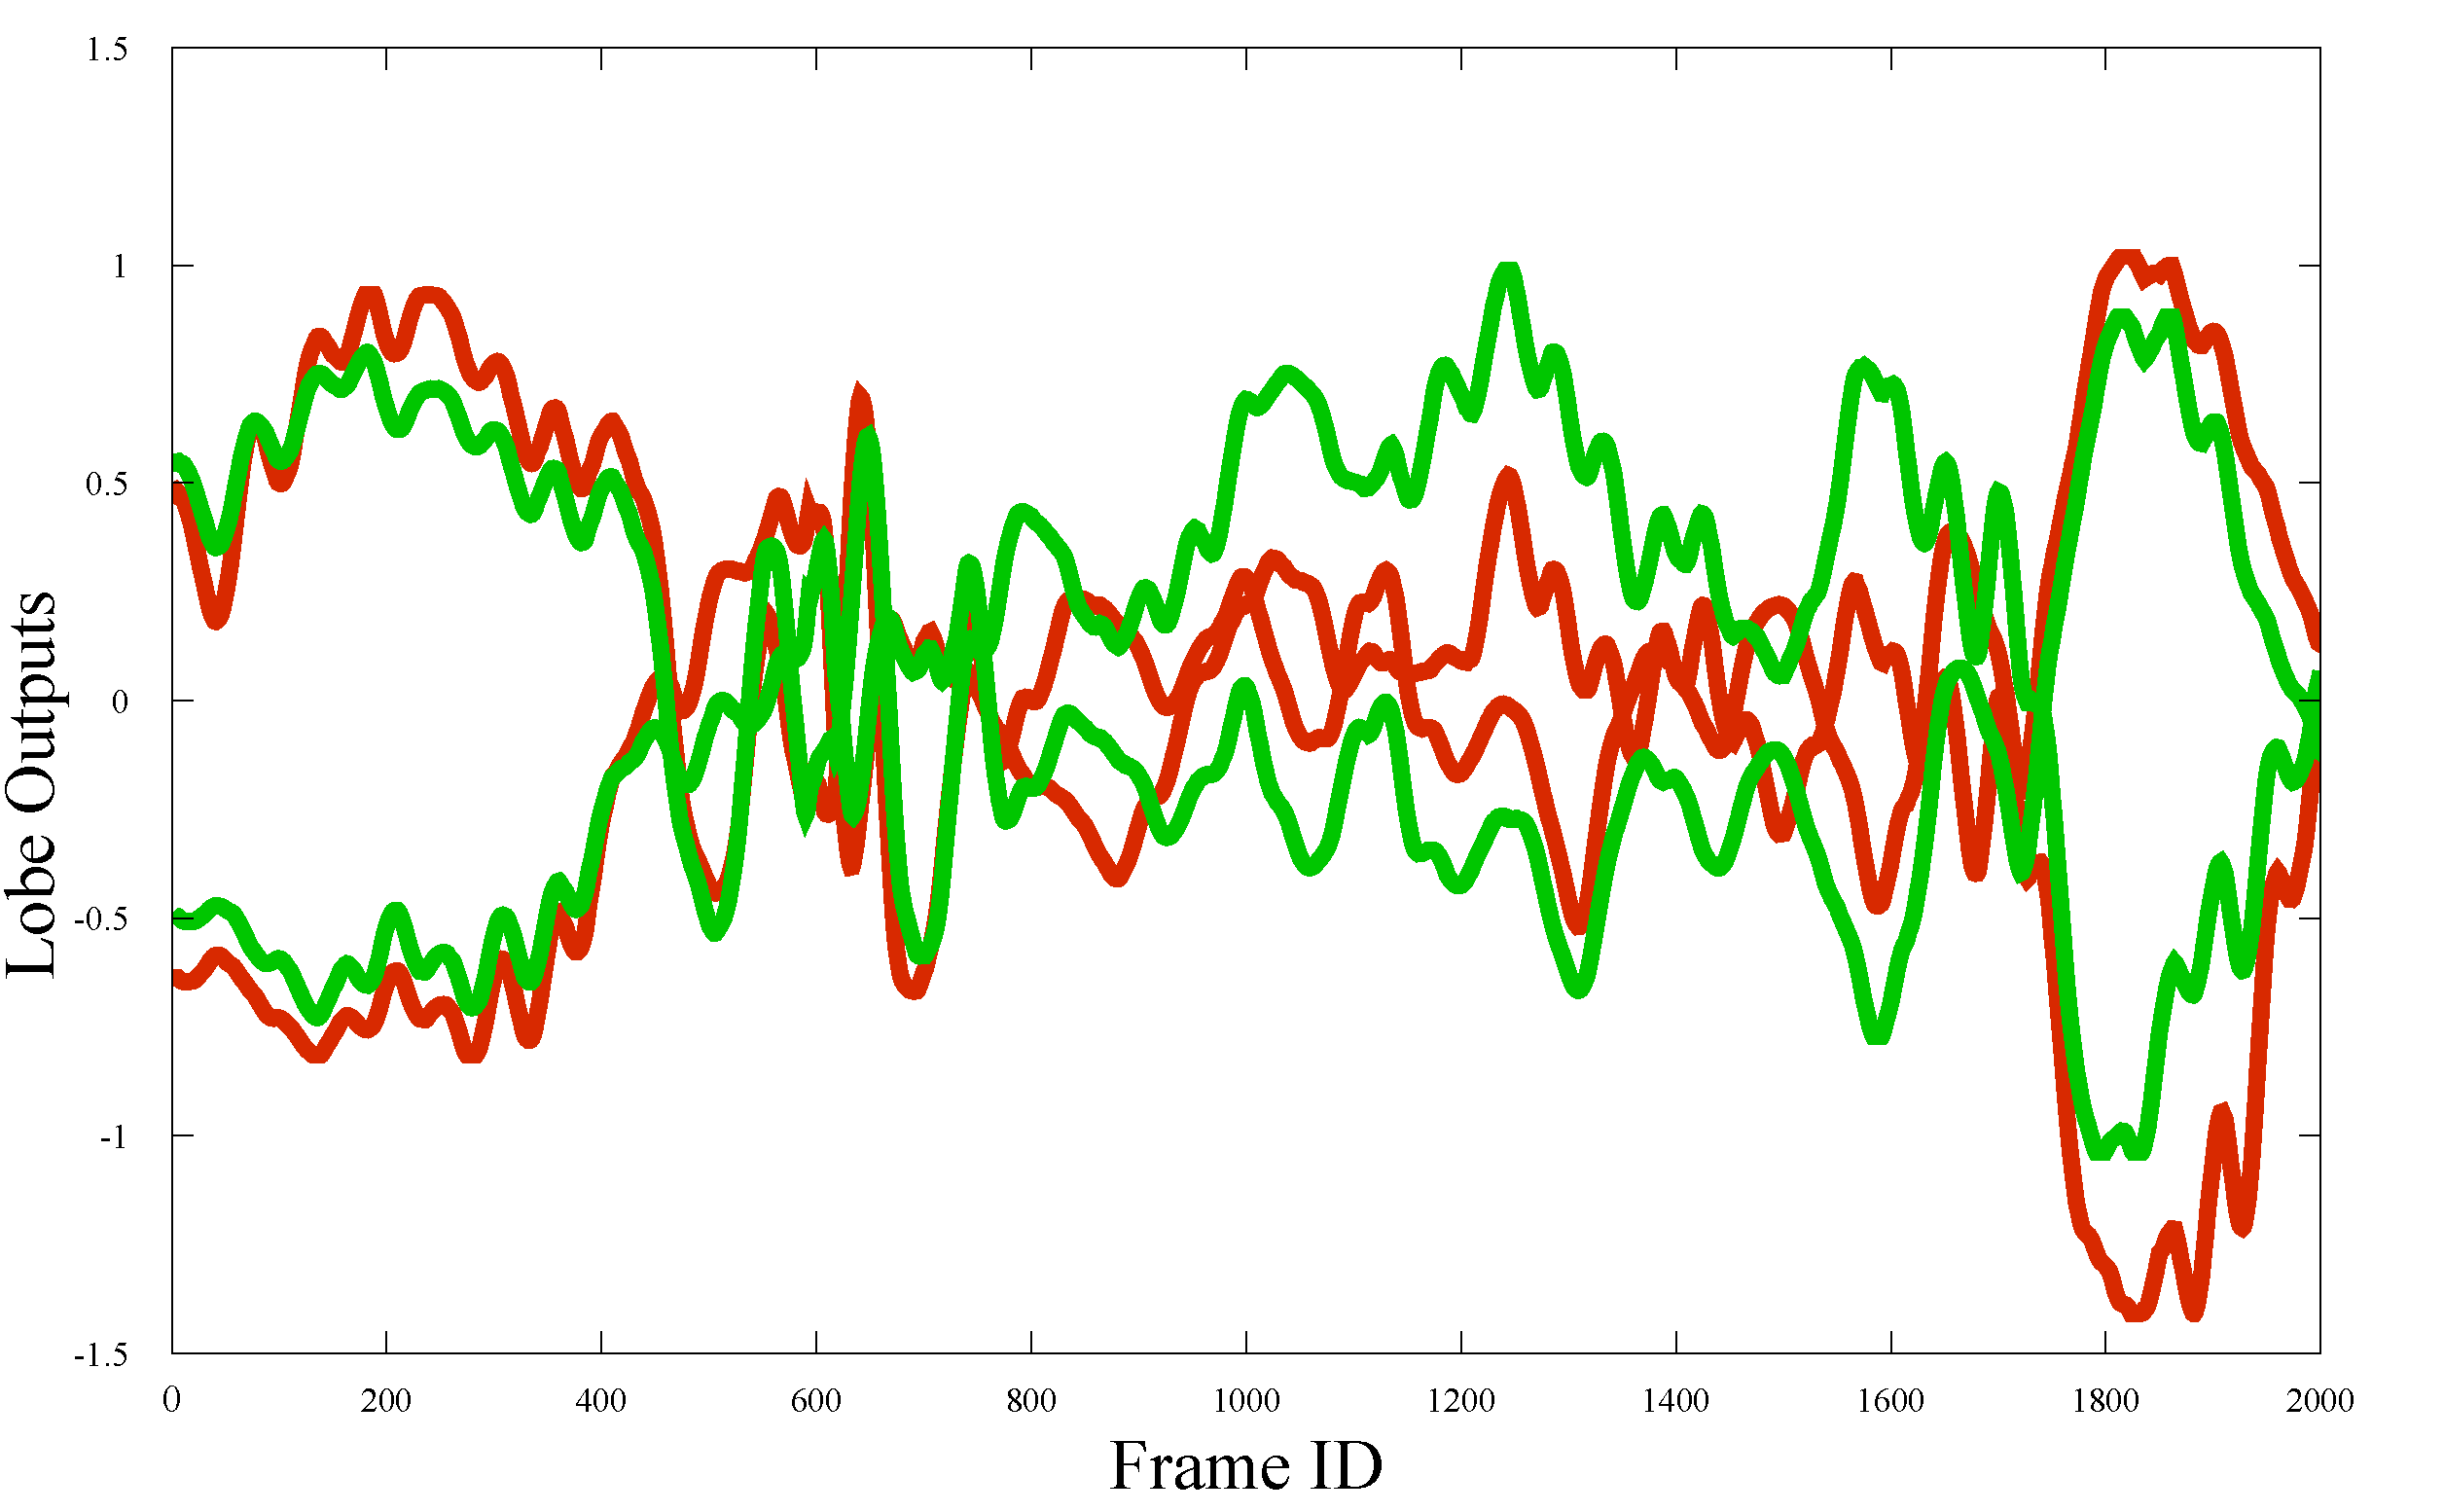
\includegraphics[width=\linewidth]{./gfx/Chapter04/Lobe1and6_red_green.pdf}
\caption{Four (of 144) representative signals acquired from a visual path; these signals encode changes in the red and green channels as a user moves through space.  The collection of signal traces at one point in time can be used to build a simple frame-level space-time descriptor: LW-COLOR. The signal amplitudes are spatially pooled temporal and spatial gradient intensities.}
\label{fig:Traces}
\end{center}
\end{figure}

At each point in time, the values over the 144 signal channels are also captured into a \textit{single} space-time descriptor per frame: LW-COLOR.  Some observations from the components of this descriptor are that a) relative ego-motion is clearly identifiable in the signals; b) stable patterns of motion may also be identified, though changes in the precise trajectory of a user could also lead to perturbations in these signals, and hence to changes in the descriptor vectors. Minor changes in trajectory might, therefore, reduce one's ability to match descriptors between users.  These observations, together with the possibility of partial occlusion, motivated the use of \textit{patch} based descriptors, so that multiple descriptors would be produced for each frame. These are introduced next.


\subsection{Local descriptors}
\label{sec:descriptors}

\subsubsection{Keypoint based SIFT (KP-SIFT)}

The original implementation of Lowe's SIFT descriptor follows the extraction of interesting points in the image that are stable to certain transformations, the ``SIFT keypoints'' \cite{Lowe2004}. As we saw in Chapter~\ref{ch:chapter2}, this descriptor is widely used across many branches of computer vision, from object recognition to motion detection and SLAM. I used the standard implementation from VLFEAT \cite{Vedaldi2008} to compute $\vec{\nabla}f(x,y;\sigma)$ where $f(x,y;\sigma)$ represents the embedding of image $f(x,y)$ within a Gaussian scale-space at scale $\sigma$. The parameter \emph{PeakThresh}, $t_p$ is used to filter out small local maxima in scale-space that might be originated by noise. Given the small size of the frames in the sequences the minimum threshold $t_p$ was set to $0$.

\subsubsection{Dense SIFT (DSIFT)}

The Dense-SIFT (DSIFT) descriptor \citep{Lazebnik2006} is a popular  alternative to keypoint based SIFT. It sacrifices some invariance properties available with keypoint-based SIFT, producing descriptors that are densely, rather than sparsely, distributed across the image. This DSIFT descriptor was calculated by  sampling of the smoothed estimate of $\vec{\nabla}f(x,y;\sigma)$.  The implementation of the VLFEAT toolbox was chosen, setting $\sigma = 1.2$, with a stride length of 3 pixels. This  yielded around $2,000$ descriptors per frame, each describing a patch of roughly $10 \times 10$ pixels.

\subsubsection{Single-frame Gabor descriptors (SF-GABOR)}
\label{sec:sf-gabor}

An alternative single-frame technique based on a tuned, odd-symmetric Gabor-based descriptor is the SF-GABOR. For this, I used the $8$-directional spatial Gabor filters previously tuned on PASCAL VOC data \cite{Everingham2009} in order to provide an implicit encoding of the orientation of local image structures.  Each filter gives rise to a filtered image plane, denoted $\mathbf{G}_{k,\sigma}$.  For each plane, I compute the discrete spatial convolution, $\mathbf{G}_{k,\sigma} \ast {\Phi}_{m,n}$, with a series of pooling functions, ${\Phi}_{m,n}$. The latter are produced by spatial sampling of the function:

\begin{equation}
\Phi(x,y;m,n) = e^{-\alpha \left [\log_e \left ( \frac{x^2+y^2}{d_n^2}\right ) \right ]^2 - \beta |\theta-\theta_m | }
\label{eq:pool1}
\end{equation}

\noindent with $\alpha = 4$ and $\beta = 0.4$. The values of $m$ and $n$ were chosen to produce 8 angular regions ($m = 0, 1, ...., 7$) at each of two distances $d_1, d_2$ away ($n=1,2$) from the centre of a spatial pooling region. These lobes were similar to those shown in Figure~\ref{fig:pooling4lwcolor}, with one additional central lobe, and used a spatial weighting pattern similar to the DAISY descriptor \cite{Winder2009}. For the central region, corresponding to $m=0$, there was no angular variation but instead a log-normal radial decay, with a limiting value at $(x,y)=(0,0)$. This arrangement yielded a total of  17 spatial pooling regions (see ``poolers'' layer in Figure~\ref{fig:IsoPool}). The resulting $17 \times 8$ fields are sub-sampled to produce dense 136-dimensional descriptors, each representing an approximate $10 \times 10$ region, and yielding around 2,000 descriptors per image frame after spatial sub-sampling. 

\begin{figure}[t]
\centering
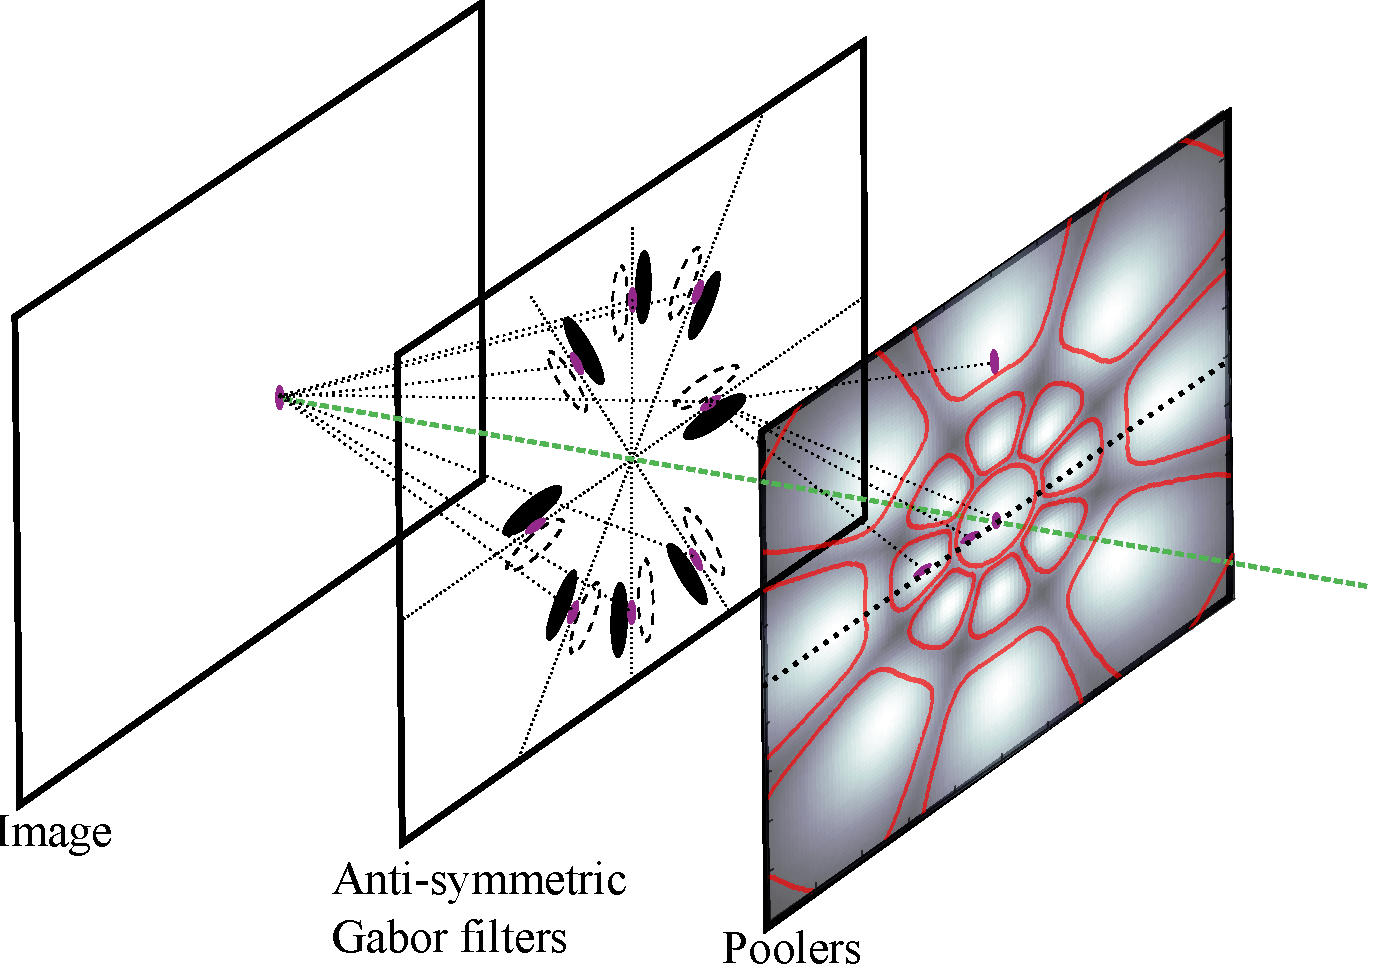
\includegraphics[width=0.7\linewidth]{./gfx/Chapter04/Layers.pdf}
\caption{The spatial pooling pattern used for single-frame Gabor filtering is based on the regions shown here.  These regions were generated by sampling Eq.~(\ref{eq:pool1}) to create pooling masks. The masks can be applied to the Gabor filtered video-frame outputs by spatial convolution, followed by sub-sampling the output every 3 pixels. See text for further details.}
\label{fig:IsoPool}
\end{figure}

These poolers were suggested by Alexiou for visual object recognition \cite{Alexiou2013}, but were thought to be good a good choice for location estimation because of the nature of the RSM navigation dataset (see Section \ref{sec:Dataset}).

In Chapter \ref{ch:chapter5} I provide another formulation for the SF-GABOR descriptor that makes use of a tensor notation. This will be needed to understand a convolutional neural network (CNN) interpretation of artificial place cell models based on the SF-GABOR descriptors.

\subsection{Space-time descriptors}

Given the potential richness available from space-time information, three distinct approaches were explored to generate space-time patch descriptors.  When generating the descriptor associated with each patch, all  approaches yield multiple descriptors per frame, and all take into account neighbouring frames in time.  In contrast to a sparse-sampling approach of a keypoint-based descriptor, all three densely sample the video sequence.  The three methods are i) HOG 3D~\cite{Klaser2008}; ii) a space-time, antisymmetric Gabor filtering process (ST-GABOR); and iii) a spatial derivative, temporal Gaussian (ST-GAUSS) filter.

\begin{enumerate}
\item The \textbf{HOG 3D} descriptor (HOG3D) \citep{Klaser2008} was introduced with the aim of extending the very successful two-di\-men\-sio\-nal histogram of oriented gradients (HOG) technique \citep{Dalal}, to space-time fields, in the form of video sequences.  HOG 3D seeks computational efficiencies by smoothing using box filters, rather than Gaussian spatial or space-time filters.  This allows three-dimensional gradient estimation across multiple scales using {\em integral video} representations, a direct extension of the integral image idea \citep{Viola2001}.  The gradients from this operation are usually performed across multiple scales.  I used the dense HOG 3D option from the implementation of the authors, and the settings yielded approximately 2,000  descriptors per frame of video. Each descriptor contained 192 elements.


\item \textbf{Space-time Gabor (ST-GABOR)} functions have been used in activity recognition, structure from motion and other applications \cite{Bregonzio2009}.  One dimensional convolution was performed between the intensity video-sequence $I(x,y,t)$ and three one-dimensional Gabor functions along either one spatial dimension i.e.\ $x$ or $y$, or along $t$ (see Eq.~\ref{eq:convolutions}).  The one-dimensional convolution  is crude, but appropriate if the videos have been downsampled. The parameters of $\sigma_x$ and $\sigma_y$ were set to be equal, and to provide one complete cycle of oscillation over approximately 5 pixels of spatial span, both for the $x$ and $y$ spatial dimensions. The filter for the temporal dimension was set to provide  around one oscillation over 9 frames.  I also explored symmetric Gabor functions, but found them rather less favourable.


\begin{equation}
\begin{array}{c}
I_1(x,y,t) = I(x,y,t) \ast g_x(x;\sigma_x) \\

I_2(x,y,t) = I(x,y,t) \ast g_y(y;\sigma_y) \\

I_3(x,y,t) = I(x,y,t) \ast g_t(t;\sigma_t)

\end{array}
\label{eq:convolutions}
\end{equation}


After performing the three separate filtering operations, each pixel of each frame is assigned a triplet of values corresponding to the result of each filtering operation.  The three values are treated as being components of a 3D vector.  Over a spatial extent of around $16 \times 16$ pixels taken at the central frame of the 9-frame support region, these vectors contribute weighted votes into descriptor bins according to their azimuth and elevations, with the weighting being given by the length of the vector.  The votes are also partitioned according to the approximate spatial lobe pattern illustrated in Figure~\ref{fig:IsoPool}. Each frame had approximately 2,000 ST-GABOR descriptors, each of 221 elements.


\item A final variant of space-time patch descriptor was designed.  This consisted of spatial derivatives in space, combined with smoothing over time \textbf{(ST-GAUSS)}.  In contrast to the strictly one-dimensional filtering operation used for the ST-GABOR descriptor, I used two $5\times 5$ gradient masks for the $x$ and $y$ directions based on derivatives of Gaussian functions, and an 11-point Gaussian smoothing filter in the temporal direction, using a standard deviation of 2.  8-directional quantisation was applied to the angles of the gradient field, and a voting process incorporating gradient magnitude was used to distribute votes across the bins of a 136-dimensional descriptor.  Like the ST-GABOR descriptor, pooling functions, similar to those shown in Figure~\ref{fig:IsoPool}, were applied.  The number of descriptors produced was the same as for the other methods using patch-level descriptions.


\end{enumerate}


\subsection{Quantisation and histogram encoding}
\label{sec:quant_and_encod}
An initial conjecture was that whole frames from a sequence could be indexed compactly, using the single-frame descriptor (LW-COLOR).  This was found to lead to disappointing performance (see Section~\ref{sec:ch4results}). For the case of many descriptors-per-frame, i.e.\ descriptors that are patch-based, there is the added problem of generating around 2,000 descriptors per frame, if dense sampling is used.  Vector quantisation (VQ) was applied to the descriptors, then histograms of quantised descriptors were used to encode each frame as a histogram of visual words \citep{Csurka2004}. The dictionary was always built by excluding the entire journey from which queries are to be taken. 

The resulting dictionaries were then used to encode the descriptors of the $M-1$ training passes and the remaining query pass. This sequence of processes is commonly known as a bag-of-visual-words (BOVW) pipeline. Two different approaches to the encoding of descriptors were taken, one based on standard $k$-means, using a Euclidean distance measure (hard assignment, ``HA''), and one corresponding to the vector of locally aggregated descriptors (VLAD) \citep{Arandjelovic}. These histograms were all $L_2$-normalised.  

In the HA case, the dataset was partitioned by selecting $M-1$ of the $M$ video sequences of passes through each possible path. These $M-1$ sequences have a total of $N$ frames. A dictionary of visual words was created by running the $k$-means algorithm on the partitioned set of training descriptors contained in the $N$ frames. The dictionary size was fixed to 4,000 in order to achieve a balance between computational time and atom stability, and allowing comparison with the work of others in related fields \cite{Chatfield2011}.

For VLAD, a $k$-means clustering was first performed using a dictionary size of 256 words. For each descriptor, sums of residual vectors were used to improve the encoding.  Further advances to the basic VLAD, which include different normalisations and multiscale approaches, are given by \cite{Arandjelovic}. 

\subsection{Localisation using histogram distances}
\label{sec:kernel_encodings}
Once histograms had been produced, a distance measurement was used to compare the similarity of histograms in a query frame with the database entries.  The query operation was simply performed by using the kernel approaches described in \cite{Vedaldi2010}.  Concretely, to compare encodings, either $\chi^2$ or Hellinger distance metrics \citep{Vedaldi2012} were used to retrieve results for HA and VLAD encoding approaches respectively. Distance comparisons were performed directly between either hard assigned bags-of-visual-words (BoVWs) or VLAD image encodings arising from collections of descriptors for each frame. 

For the $M-1$ videos captured over each path in the database, the queries were constructed from the remaining path. The histogram of each query frame, $H_q$, resulted in $M-1$ separate comparison vectors containing scores.  By using these kernel-based comparisons (which are always positive, and act in the opposite way of a distance metric), one can identify the best matching frame, $\hat{f}$, from pass, $\hat{p}$, across all of the $M-1$ vectors.  This may be expressed as: 
\begin{equation}
L(\hat{p},\hat{f}) = \underset{p,f}{\textrm{argmax}} \lbrace K_{D}(H_q,H_{p,f})\rbrace
\label{eq:argmax}
\end{equation}
where $H_{p,f}$ denotes the series of normalised histogram encodings, indexed by $p$ drawn from the $M-1$ database passes, and $f$ denotes the frame number within that pass. $K_D$ denotes the so-called \textit{kernelised} version of distance measure \cite{Vedaldi2010}.  To measure the localisation error, I used the ground-truth estimates that were acquired at the same time as the videos. The estimated position of a query, $L$, was simply taken to be that of the best match given by Eq. (\ref{eq:argmax}).  However, in a more robust implementation, checks could be done that would require similar matches in neighbouring frames, both in query and pass.
%%END EDIT BLOCK


%------------------------------------------------------------------------- 
\section{The RSM dataset}
\label{sec:Dataset}
In order to allow different approaches to be compared, and as a community resource to develop appearance-based methods for visual localisation, the \textit{RSM dataset} was constructed and is made publicly available at \url{http://rsm.bicv.org} \cite{Rivera-RubioRSM}. In this section I will briefly review the existing datasets for visual localisation and explain the motivations behind the creation of the RSM dataset.


\subsection{Existing datasets}

Datasets for evaluating visual localisation methods have often been limited to demonstrate the performance of particular metrics such as point cloud accuracy~\cite{Huitl2012, nardi2014introducing}. This has led to a number of datasets that were difficult to adapt to new work and different performance metrics, or simply unavailable because they were not released to the community~\cite{Matsumoto1996,Ohno1996,Tang2001}.

\paragraph{Historical datasets}

The early work described in Section \ref{subsec:early_works} used custom-planned datasets for their specific evaluation objectives. This led to datasets \cite{Matsumoto1996,Ohno1996,Tang2001} containing very short sequences, of few meters of length, that could not be used to assess localisation performance at realistic scale of indoor human navigation.

\paragraph{SLAM datasets and the NAVVIS dataset}

SLAM  da\-ta\-sets, found in the robotics community, have a variety of scopes and recorded distances: large indoor spaces \cite{sturm12iros}, outdoor i\-ti\-ne\-ra\-ries \cite{Bosse2004}, and up to the scale of a few km car ride \cite{Simpson2011}. They are also heterogeneous in terms of the precision and nature of the ground truth: some use GPS, others the Microsoft Kinect to capture depth \cite{sturm12iros}, while others use the Vicon motion capture system. While the ground truth is often precise (up to the level of GPS, Kinect or Vicon precision), these have usually targeted outdoor comparisons; indoor comparisons focused at geometric reconstruction or pose estimation rather than localisation.

To the best of our knowledge, with the exception of NAVVIS \cite{Huitl2012}, SLAM datasets have had rather restricted distances, not addressing real-world navigation on the scale of large buildings. The NAVVIS project described in Section \ref{subsec:visual_paths} first introduced a more generic dataset that could evaluate visual localisation and navigation at human scale for robotic applications. The RSM dataset takes the evaluation and the principle closer to the assistive context than the robot-centric approach of the NAVVIS team: our data and evaluation context introduces the particularities of human motion, both from hand-held and a wearable camera.

\subsection{The RSM dataset of visual paths}

I have previously defined a \textit{visual path} as the video sequence captured by a moving person in executing a journey along a particular physical path. For the construction of our dataset, the \textit{RSM dataset of visual paths}, a total of 60 videos were acquired from 6 corridors of a large building, the Royal School of Mines at Imperial College London. A layout of the trajectories is reproduced in Figure \ref{fig:map_and_legend}. In total, 3.05 km of data is contained in this dataset at natural indoor walking speeds.  For each corridor, ten passes (i.e.\ 10 separate visual paths) are obtained. These are acquired with two different devices with 30 videos each. One device was an LG Google Nexus 4 phone running Android 4.4.2.  The video data was acquired at approximately 24-30 fps at two different resolutions, $1280 \times 720$ and $1920\times 1080$ pixels.  The second device was a Google Glass (Explorer edition) acquiring at a resolution of $1280 \times 720$, and at a frame rate of 30 fps. Table~\ref{tbl:Datasets} summarises the acquisition.  As can be seen, the length of the sequences varies within some corridors, due to a combination of different walking speeds and/or different frame rates. Lighting also varied, due to a combination of daylight/night-time acquisitions, and occasional prominent windows that represent strong lighting sources in certain parts of some corridors.  Changes were also observable in some videos from one pass to another, due to the presence of changes and occasional appearance from people. In total, more than 90,000 frames of video are labelled with positional ground truth in a path relative manner. 

\subsection{Ground truth Acquisition}

A surveyor's wheel (Silverline) with a precision of 10 cm and error of $\pm 5\%$ was used to record distance, but was modified by wiring its encoder to a Raspberry Pi model B running a number of measurement processes. The Pi was synchronised to network time using the network time protocol (NTP) enabling synchronisation with timestamps in the video sequence.  Because of the variable-frame rate of acquisition, timestamp data from the video was used to align ground-truth measurements with frames. This data was used to access the accuracy of associating positions along journeys through frame indexing and comparison.


\begin{figure}[t]
\centering
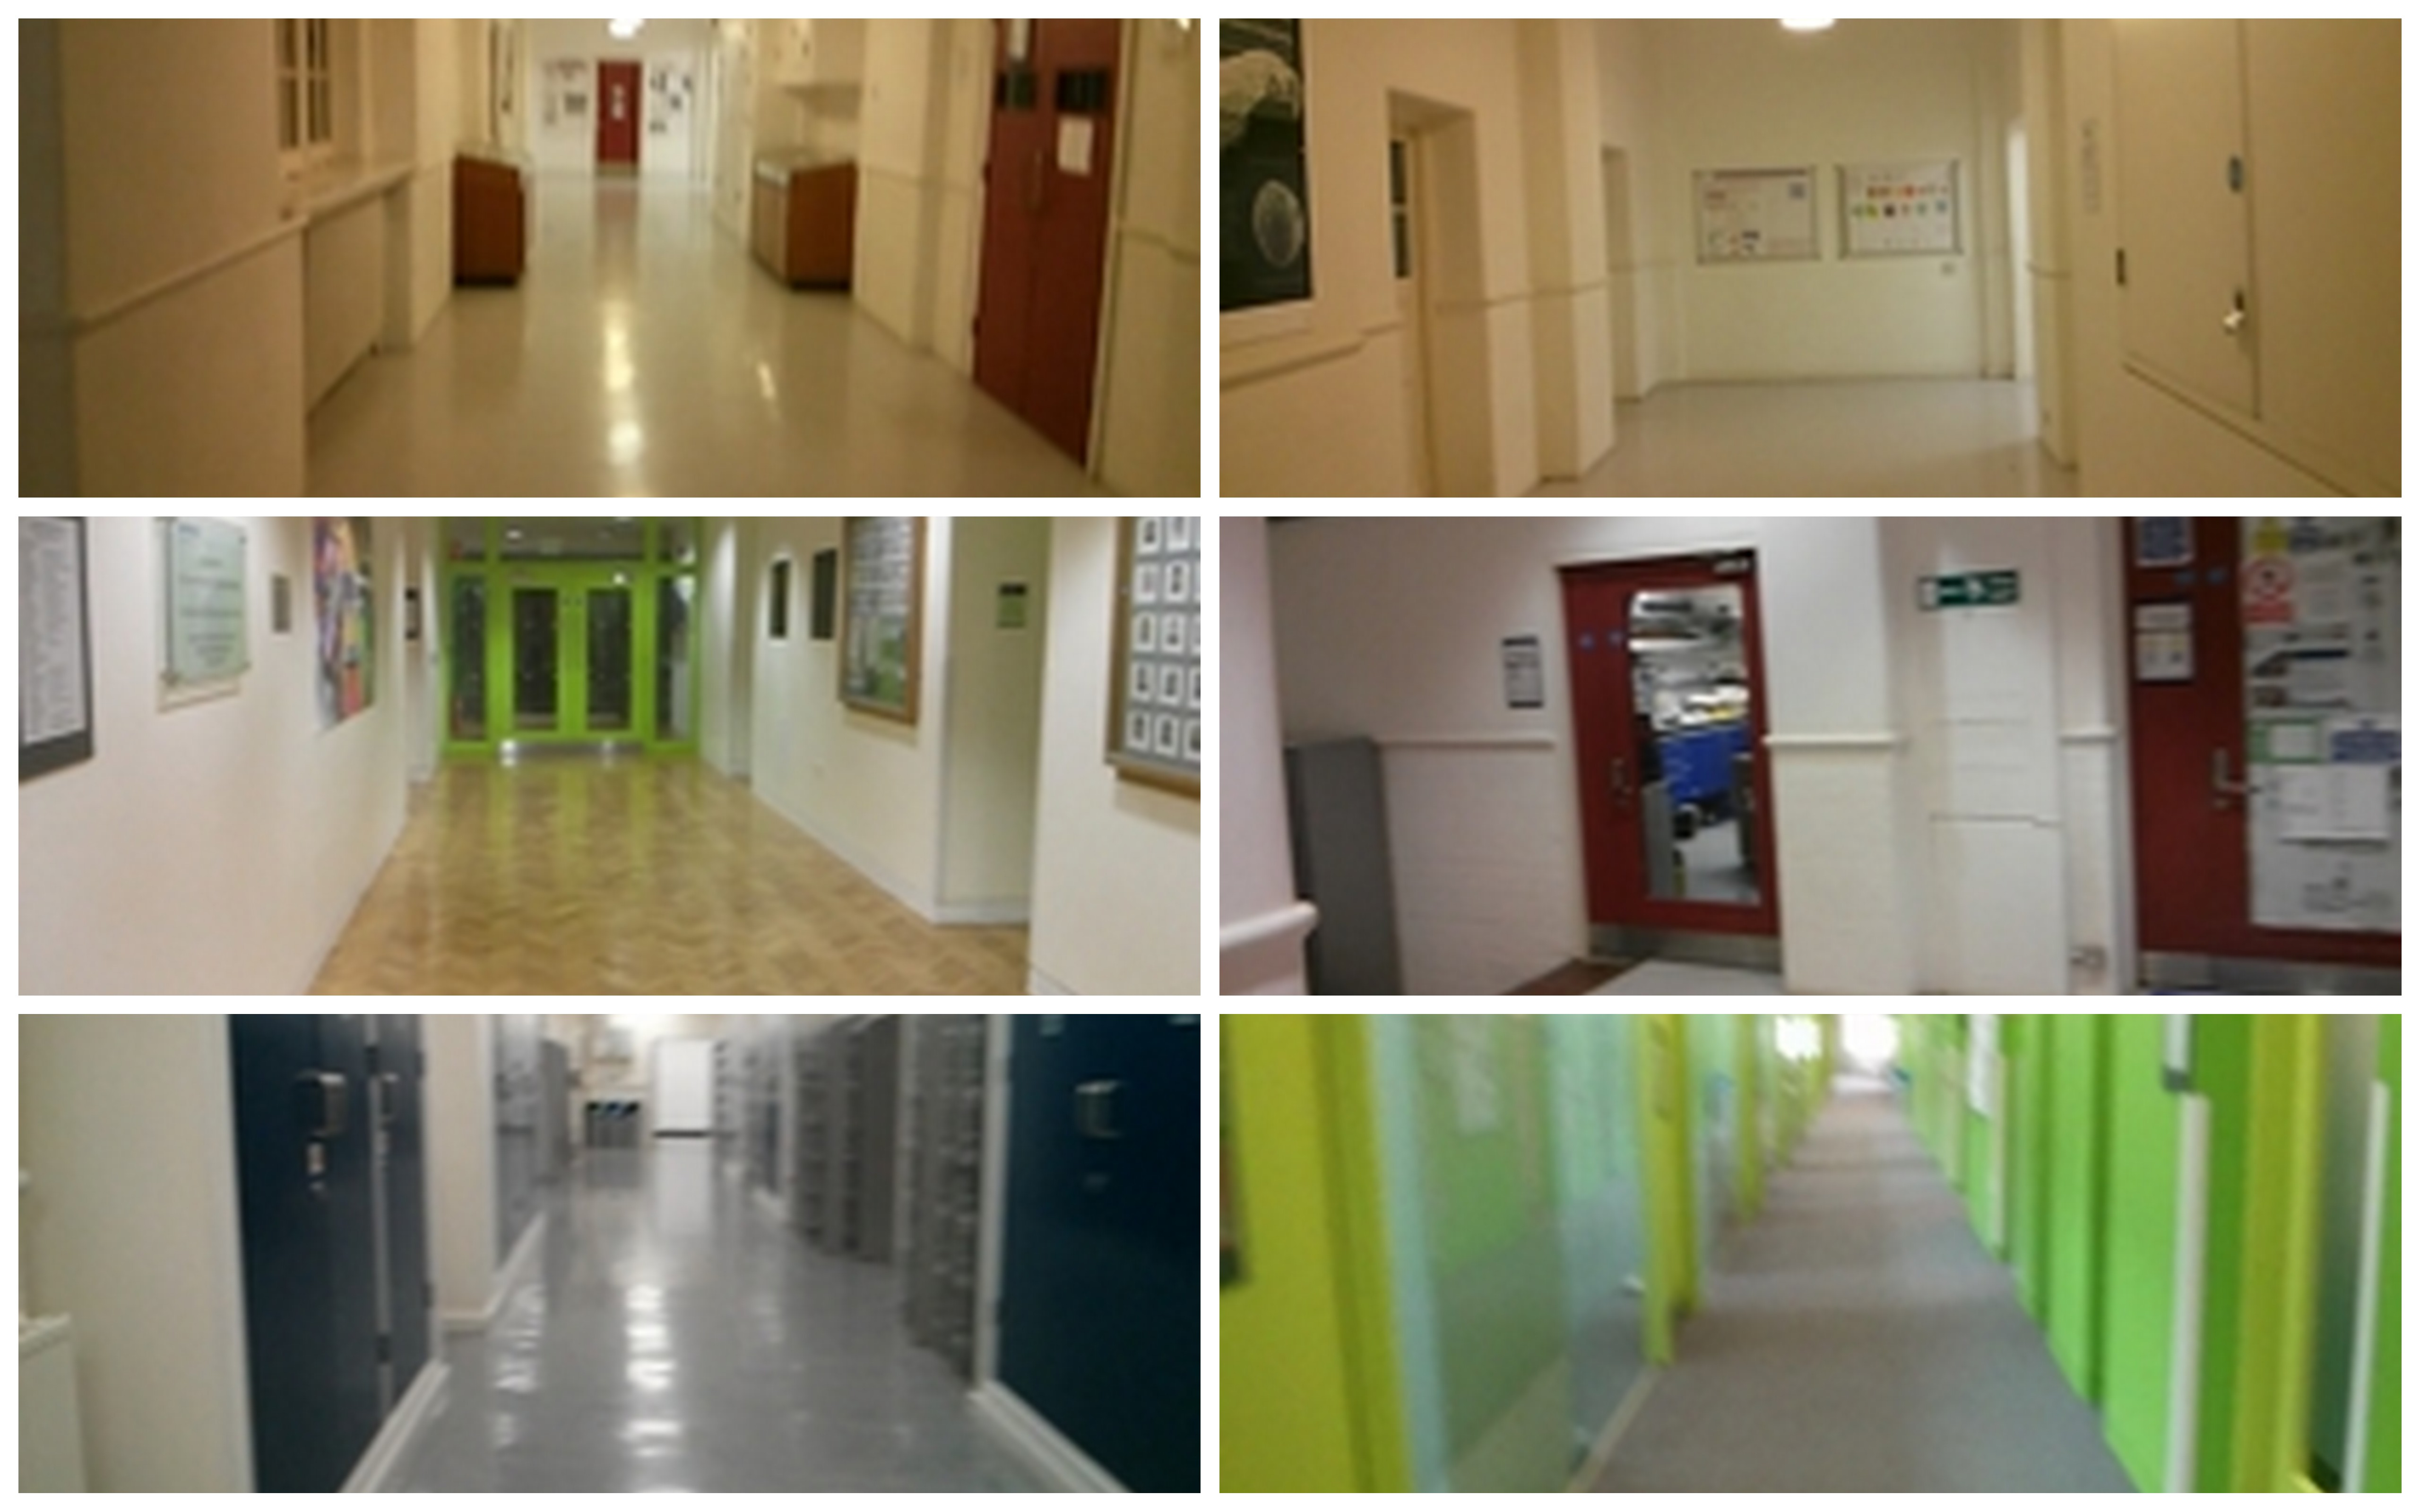
\includegraphics[width=\linewidth]{./gfx/Chapter04/rsm_collage.jpg}
\caption{A ``collage'' depicting a thumbnail of each corridor of the RSM dataset. From top left to bottom right C1, C2, ..., C6.}
\label{fig:RSMcollage}
\end{figure}


\begin{table}[ht]


\begin{center}

\centering
    \begin{tabular}{l c c c c c c c}
    \hline
    & \multirow{2}{*}{\bf{Photo}} & \multicolumn{3}{c}{\bf{Length (m)}} & \multicolumn{3}{c}{\bf{No. of frames}}  \\ \cline{3-8}
             & ~     & Avg    & Min   & Max   & Avg              & Min  & Max  \\ \hline
    C1       & \begin{minipage}{.2\textwidth}
      			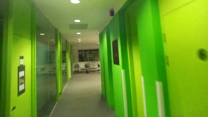
\includegraphics[width=\linewidth]{./gfx/Chapter04/table/1.jpg}
			   \end{minipage}
			        & 57.9  & 57.7 & 58.7 & 2157         & 1860 & 2338 \\ \hline
    C2       & \begin{minipage}{.2\textwidth}
      			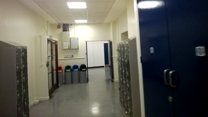
\includegraphics[width=\linewidth]{./gfx/Chapter04/table/2.jpg}
			   \end{minipage}
         & 31.0  & 30.6 & 31.5 & 909          & 687  & 1168 \\ \hline
    C3       & \begin{minipage}{.2\textwidth}
      			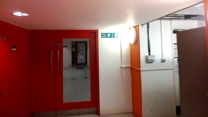
\includegraphics[width=\linewidth]{./gfx/Chapter04/table/3.jpg}
			   \end{minipage}
			        & 52.7  & 51.4 & 53.3 & 1427         & 1070 & 1777 \\ \hline
    C4       & \begin{minipage}{.2\textwidth}
      			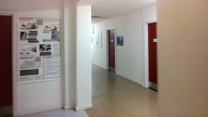
\includegraphics[width=\linewidth]{./gfx/Chapter04/table/4.jpg}
			   \end{minipage}
			        & 49.3  & 46.4 & 56.2 & 1583         & 1090 & 2154 \\ \hline
    C5       & \begin{minipage}{.2\textwidth}
      			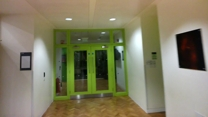
\includegraphics[width=\linewidth]{./gfx/Chapter04/table/5.jpg}
			   \end{minipage}
			        & 54.3  & 49.3 & 58.4 & 1782          & 1326 & 1900 \\ \hline
    C6       & \begin{minipage}{.2\textwidth}
      			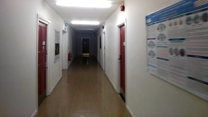
\includegraphics[width=\linewidth]{./gfx/Chapter04/table/6.jpg}
			   \end{minipage}
			        & 55.9  & 55.4 & 56.4 & 1471          & 1180 & 1817 \\ \hline \hline
	\multicolumn{2}{l}{Total}      & \multicolumn{3}{c}{3.042 km} & \multicolumn{3}{c}{90,302 frames} \\ \hline
    \end{tabular}
\end{center}
\caption{A summary of the dataset with thumbnails}
\label{tbl:Datasets}
\end{table}


\section{Experiments}
\label{sec:exp_methods}

\subsection{Performance Evaluation}

The methods for a) describing spatial or space-time structure, b) indexing and comparing the data are summarised in Table~\ref{tbl:Methods}. The choice of parameters was selected to allow a) as consistent a combination of methods as possible, allowing fair comparisons of the effect of one type of encoding or spatio-temporal operator to be isolated from others b) to select parameter choices close to other research in the area, e.g.\ for image categorisation, the chosen dictionary sizes of $\approx 256$, $\approx 400$ and $\approx 4000$ words are common. 

\begin{table}

\small
\centering
    \begin{tabular}{l p{0.5cm} p{0.9cm} p{0.5cm} p{2.5cm} c }
    \hline
    \textbf{Method}              & \textbf{ST} & \textbf{Dense} & \textbf{Dim}  & \textbf{Encoding}      & \textbf{Metric}    \\ \hline
    \multirow{2}{*}{KP-SIFT} & \multirow{2}{*}{No} & \multirow{2}{*}{No} & \multirow{2}{*}{128}     & HA-4000  &   $\chi^2$    \\ \cline{5-6} 
        ~                   & ~      & ~           & ~      & VLAD-256 & Hellinger \\ \hline
    \multirow{2}{*}{DSIFT} & \multirow{2}{*}{No} & \multirow{2}{*}{Yes} & \multirow{2}{*}{128}     & HA-4000  &   $\chi^2$    \\ \cline{5-6}
    ~                   & ~      & ~           & ~      & VLAD-256 & Hellinger \\ \hline
    \multirow{2}{*}{SF-GABOR} & \multirow{2}{*}{No}               & \multirow{2}{*}{Yes}  & \multirow{2}{*}{136}  & HA-4000  & $\chi^2$      \\  \cline{5-6}
    ~                   & ~      & ~           & ~      & VLAD-256 & Hellinger \\ \hline
    LW-COLOR           & Yes & No & 144           & N/A       \\ \hline
    \multirow{2}{*}{ST-GABOR}          & \multirow{2}{*}{Yes}              & \multirow{2}{*}{Yes}  & \multirow{2}{*}{221}  & HA-4000  & $\chi^2$      \\  \cline{5-6}
    ~                   & ~      & ~           & ~      & VLAD-256 & Hellinger \\ \hline
    \multirow{2}{*}{ST-GAUSS}           & \multirow{2}{*}{Yes}              & \multirow{2}{*}{Yes}  & \multirow{2}{*}{136}  & HA-4000  & $\chi^2$      \\  \cline{5-6}
    ~                   & ~      & ~           & ~      & VLAD-256 & Hellinger \\ \hline
    \multirow{2}{*}{HOG3D}               & \multirow{2}{*}{Yes}              & \multirow{2}{*}{Yes} & \multirow{2}{*}{192}   &  HA-4000  & $\chi^2$      \\  \cline{5-6}
    ~                   & ~       & ~          & ~      & VLAD-256 & Hellinger \\ \hline
    \end{tabular}
    \normalsize
    
    \caption{A summary of the different encoding methods and their relationships to different descriptors. The number of elements of each descriptor is also reported (\textbf{Dim}).}
\label{tbl:Methods}
\end{table}


\subsubsection{Error distributions}
\label{sec:CDFs}
Error distributions allow us to quantify the accuracy of being able to estimate {\em locations} along physical paths within the RSM dataset described in Section~\ref{sec:Dataset}. To generate the error distributions, the following method was used: 

Using the kernels introduced in Section~\ref{sec:kernel_encodings}, location inference was attempted. One kernel is shown in Figure~\ref{fig:kernel}, where the rows represent each frame from the query pass, and the columns represent each frame from one of the remaining database passes of that corridor. The values of the kernel along a row represent a ``score'' between a query and different database frames given by applying the kernel mapping functions described in \citep{Vedaldi2012} for the $\chi^2$ and Hellinger kernel depending on the case. In this experiment, the position of the best matching database image to the query frame was calculated. The absolute error between this and the ground truth $|\epsilon|$, in m, is then determined. I used the ground-truth information acquired as described in Section \ref{sec:Dataset}. 

In order to characterise the reliability of such scores, bootstrap estimates of error distributions were obtained by using 10 million trials. Specifically, permuting the paths that are held in the database and randomly selecting queries from the remaining path, these error distributions in localisation can be obtained. The bootstrap estimates consisted of 1,000 repeated runs with random selections of 10,000 frames each, revealing the variability in these estimates, including that due to different numbers of paths and passes being within the database. In Appendix \ref{appendixCDF} I describe the algorithm to generate the cumulative distribution functions (CDFs) in more detail. The distribution of the errors gives us a probability density estimate, from which one can get the cumulative distribution function (CDF) $P(|\epsilon| \leq x)$. 

The outcome is shown in Figure~\ref{fig:CDFall}, where the variability in the lines indicate the range of the results obtained during permuting the observations as described above.

\begin{figure}[h]
\centering
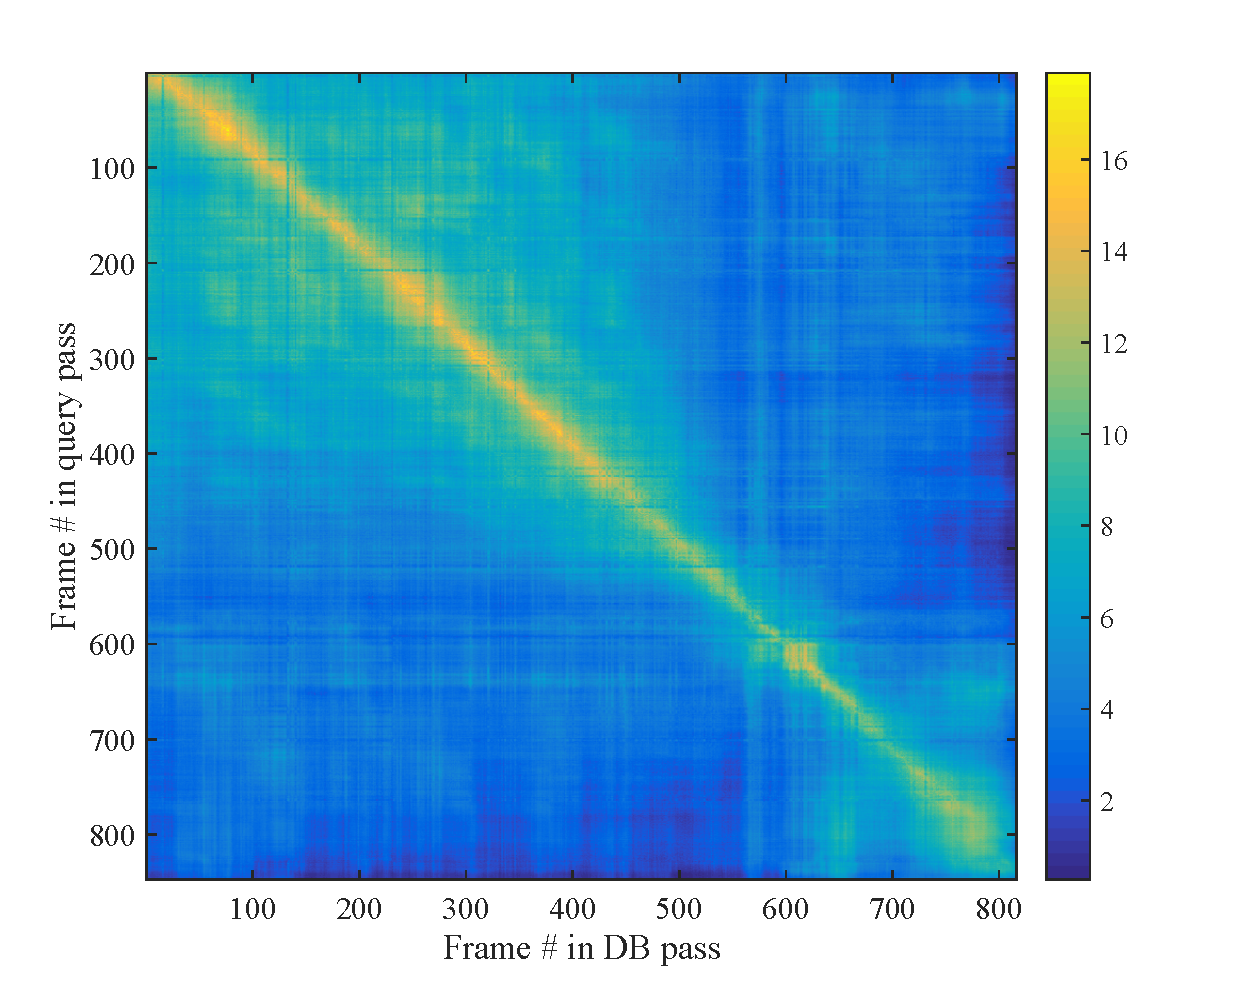
\includegraphics[width=\linewidth]{./gfx/Chapter04/kernel.pdf}
\caption{Example of a $\chi^2$ kernel produced by hard assignment and using the SF-GABOR descriptors when querying with pass P1 of corridor C2 against a database comprised of passes P2-10.}
\label{fig:kernel}
\end{figure}

Let us consider the idea of crowdsourcing journey information from many pedestrian journeys through the same corridors. This approach to evaluating the error thus makes sense:  all previous journeys could be indexed and held in the database; new journey footage would be submitted as a series of query frames (see Figure~\ref{fig:pathexample} from Chapter \ref{ch:chapter2}).    

All the results were generated with a downsampled version of the videos at $208 \times 117$ pixels. 




%------------------------------------------------------------------------- 
\section{Results}
\label{sec:ch4results}

I calculated the average absolute positional error (in metres) and the standard deviation of the absolute positional errors across the provided dataset, and these are shown in Table~\ref{Table:summaries}. For these errors, all queries, by a leave-one-out strategy, have been used, but there is otherwise no random sampling of the queries.  Standard deviations of the absolute errors are also provided.  Table~\ref{Table:summaries} also provides the Area-Under-Curve (AUC) values obtained from the CDFs of Figure~\ref{fig:CDFglobal}.


\begin{figure}[h!]
\subfloat[]{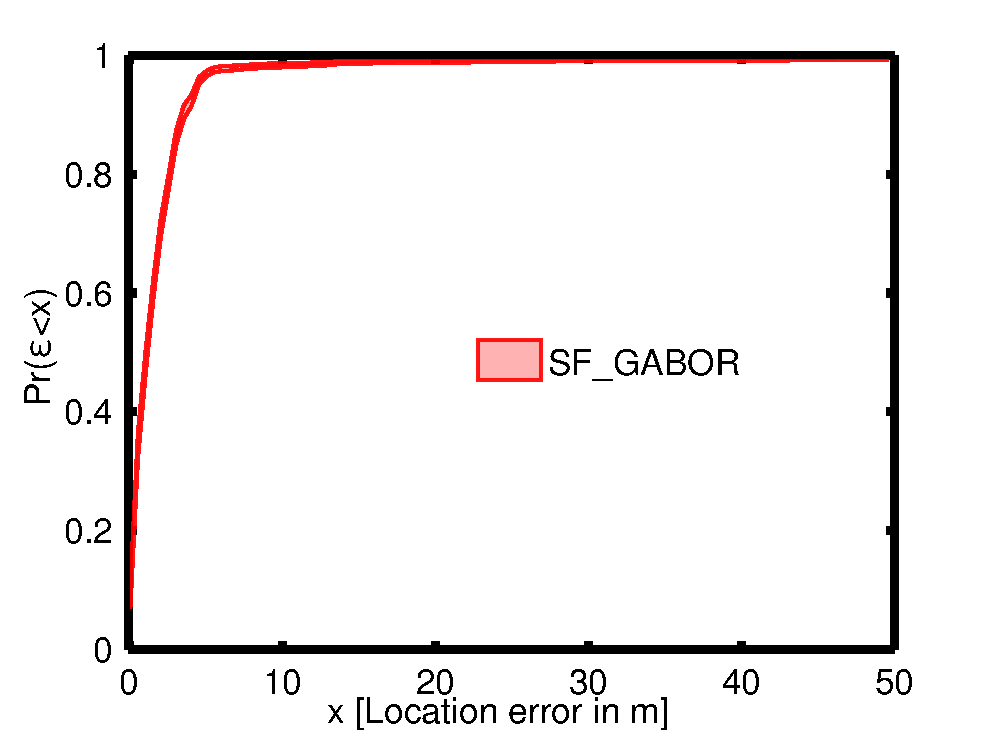
\includegraphics[width=0.5\textwidth]{./gfx/Chapter04/CDF_Figs/SF_GABOR.pdf}}	\subfloat[]{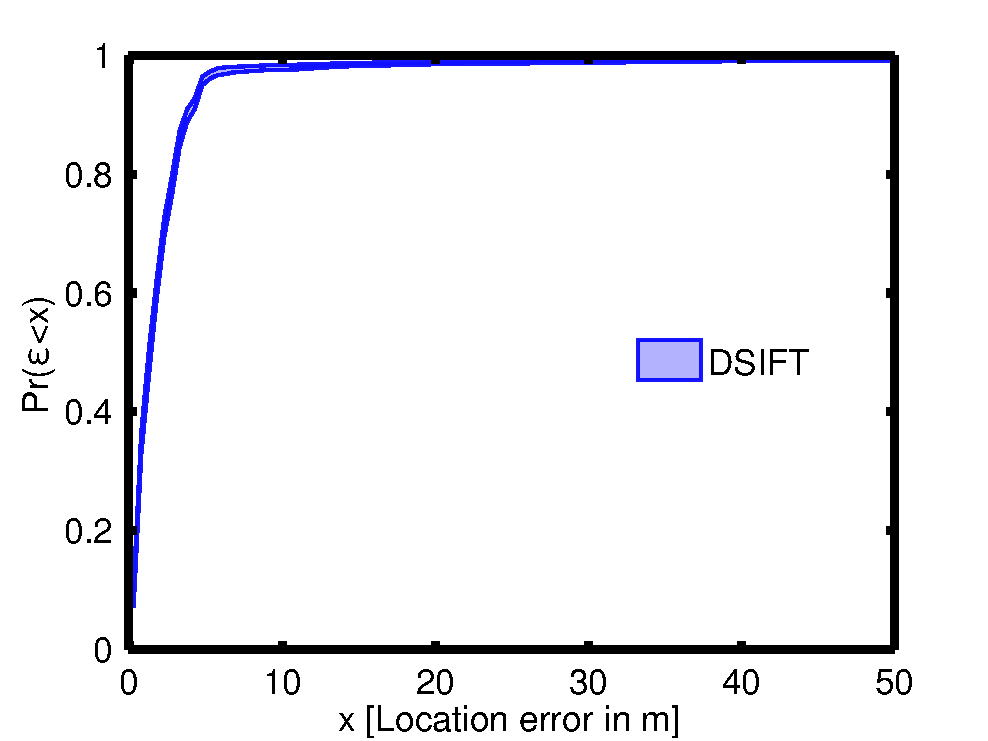
\includegraphics[width=0.5\textwidth]{./gfx/Chapter04/CDF_Figs/DSIFT.pdf}}\\
\subfloat[]{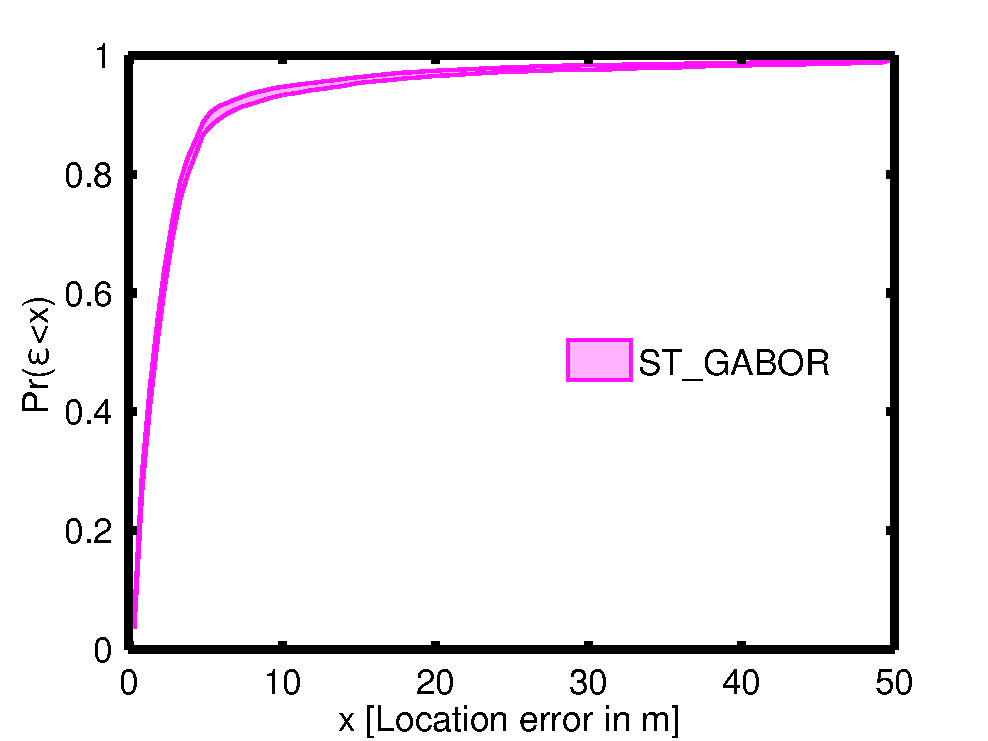
\includegraphics[width=0.5\textwidth]{./gfx/Chapter04/CDF_Figs/ST_GABOR.pdf}}
\subfloat[]{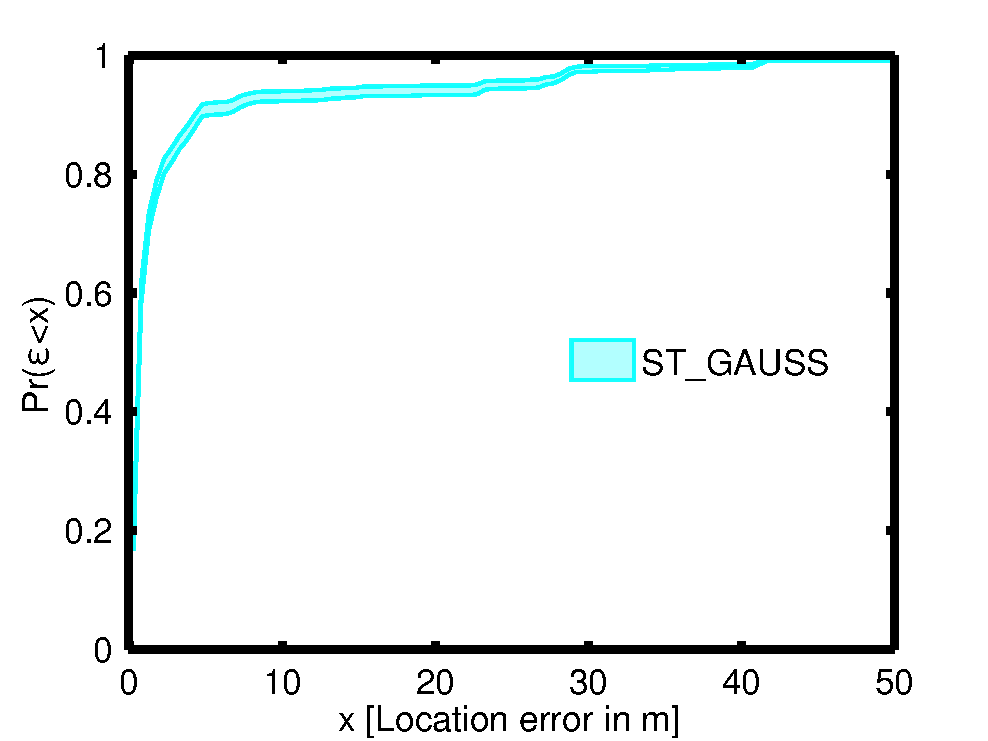
\includegraphics[width=0.5\textwidth]{./gfx/Chapter04/CDF_Figs/ST_GAUSS.pdf}}\\
\subfloat[]{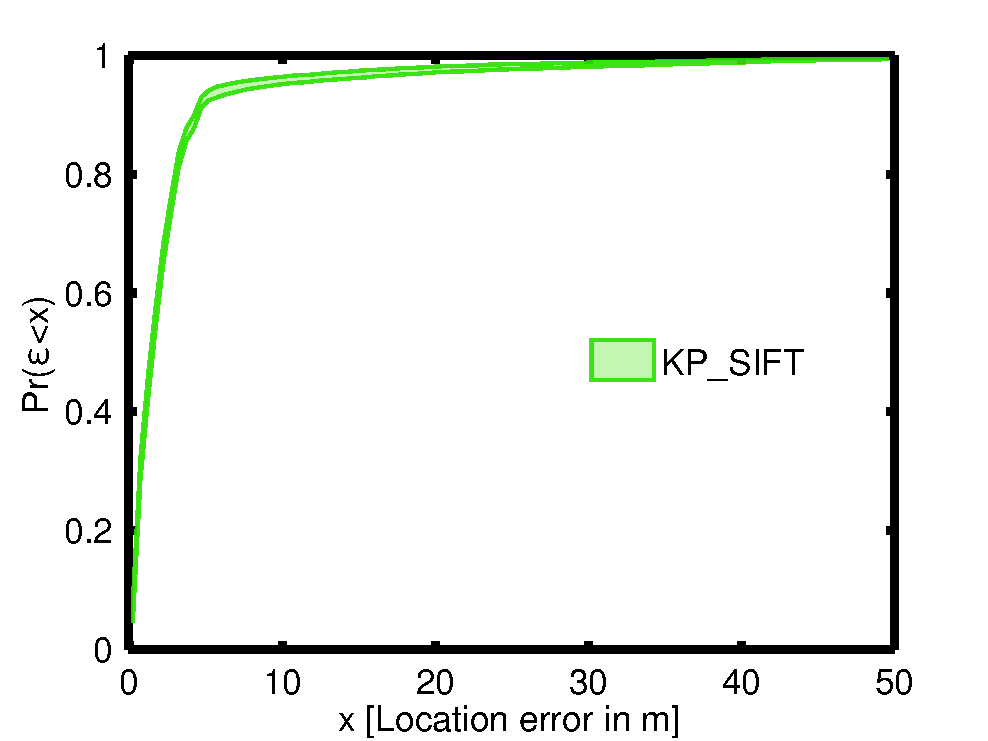
\includegraphics[width=0.5\textwidth]{./gfx/Chapter04/CDF_Figs/KPSIFT.pdf}}
\subfloat[]{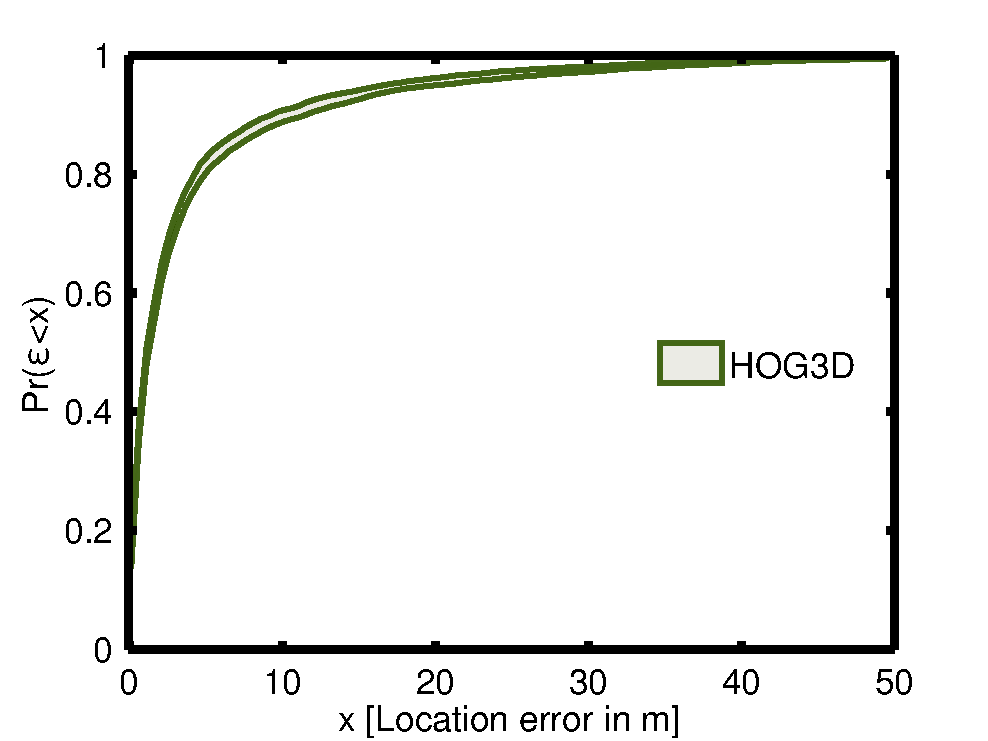
\includegraphics[width=0.5\textwidth]{./gfx/Chapter04/CDF_Figs/HOG3D.pdf}}
\caption{Comparison between the error distributions obtained with the different methods. Note the high reproducibility of the performance results. The origin of the variability within each curve is explained in Section \ref{sec:CDFs}.}
\label{fig:CDFglobal}
\end{figure}

\begin{figure}
\centering
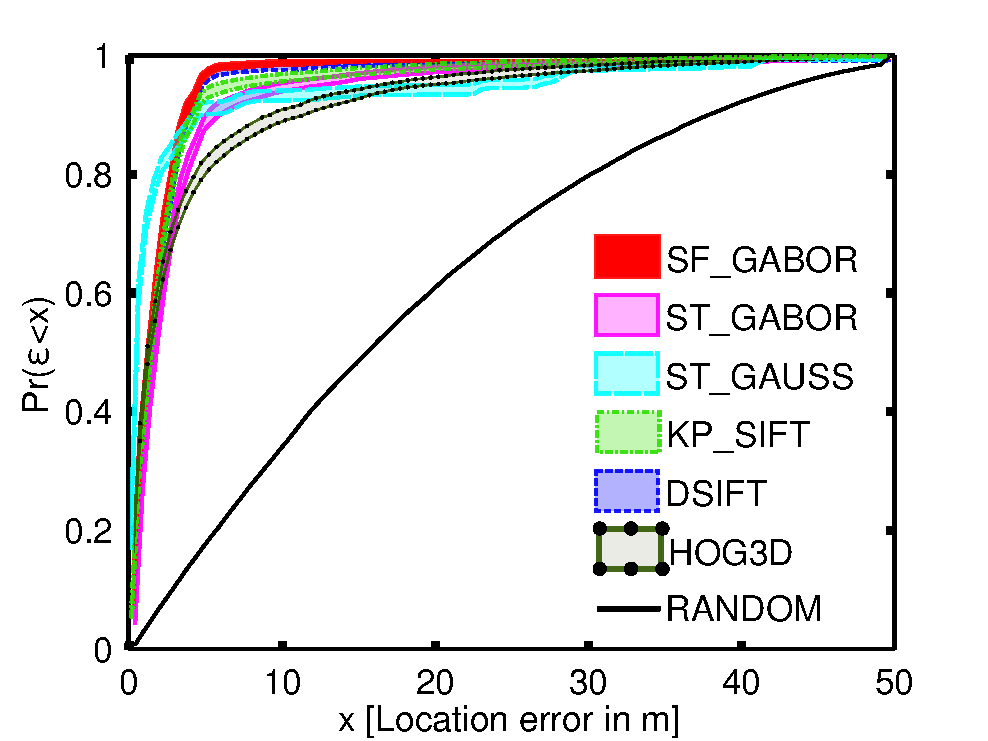
\includegraphics[width=\textwidth]{./gfx/Chapter04/CDF_Figs/all.pdf}
\caption{Comparison between the error distributions obtained with the different methods. The results for a random frame test (RANDOM) were introduced as a ``sanity check''}
\label{fig:CDFall}
\end{figure}



%\begin{figure}[h]
%\begin{center}
%\begin{subfigure}[b]{.6\linewidth}
%\captionsetup{skip=0pt} % local setting for this subfigure
%
%\begin{subfigure}[b]{\linewidth}
%
%	\begin{subfigure}[b]{.45\linewidth}
%	\centering
%	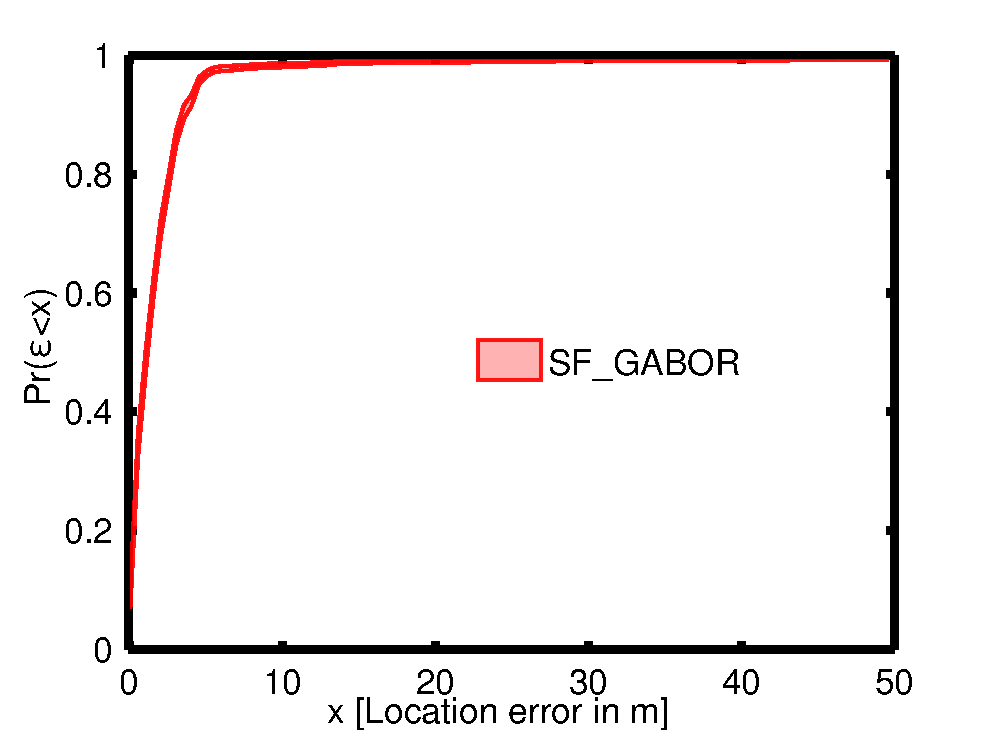
\includegraphics[width=\textwidth]{./gfx/Chapter04/CDF_Figs/SF_GABOR.pdf}\caption{}\label{fig:CDFa}
%	\end{subfigure}
%	\begin{subfigure}[b]{.45\linewidth}
%	\centering
%	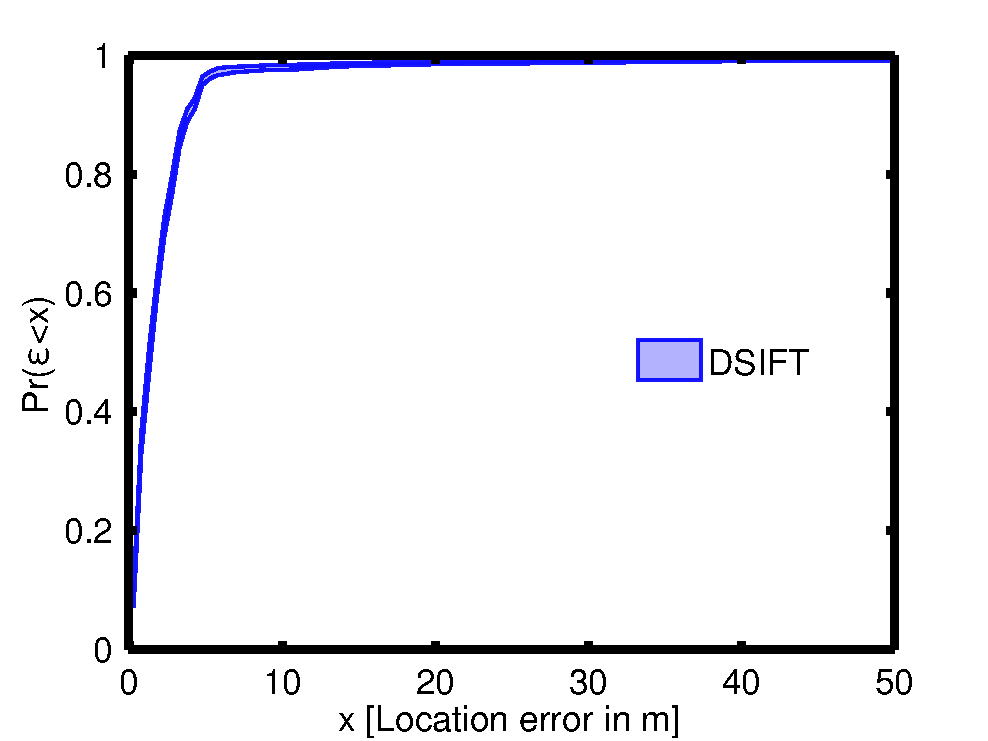
\includegraphics[width=\textwidth]{./gfx/Chapter04/CDF_Figs/DSIFT.pdf}\caption{}\label{fig:CDFb}
%	\end{subfigure}
%	
%\end{subfigure}
%
%
%\begin{subfigure}[b]{\linewidth}
%
%\begin{subfigure}[b]{.45\linewidth}
%\centering
%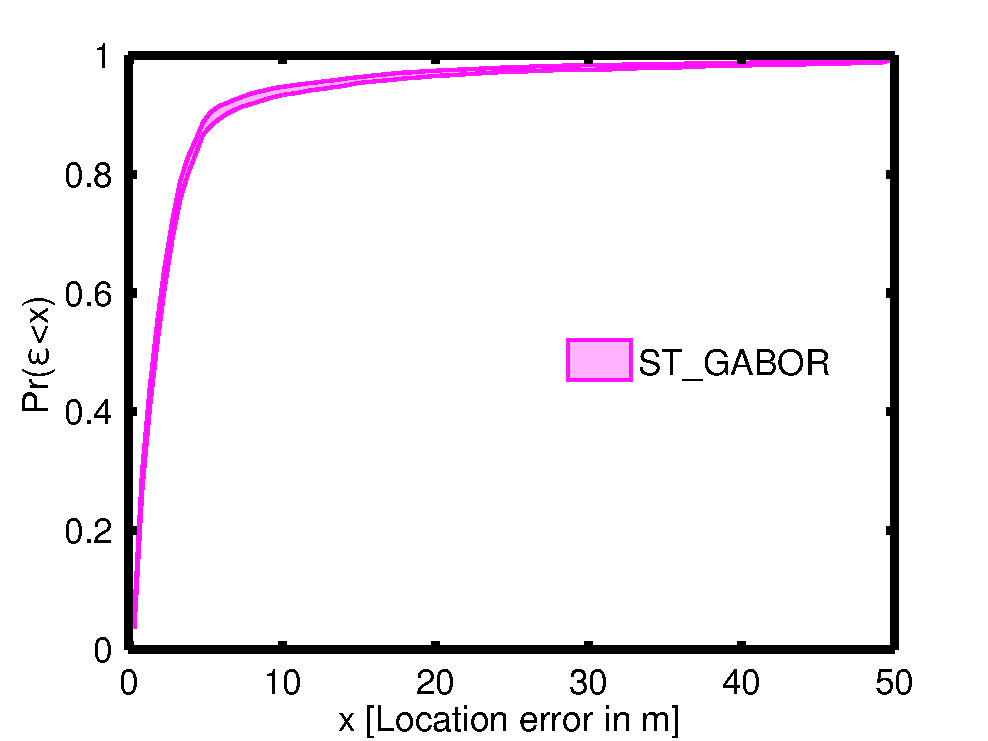
\includegraphics[width=\textwidth]{./gfx/Chapter04/CDF_Figs/ST_GABOR.pdf}\caption{}\label{fig:CDFc}
%\end{subfigure}
%\begin{subfigure}[b]{.45\linewidth}
%\centering
%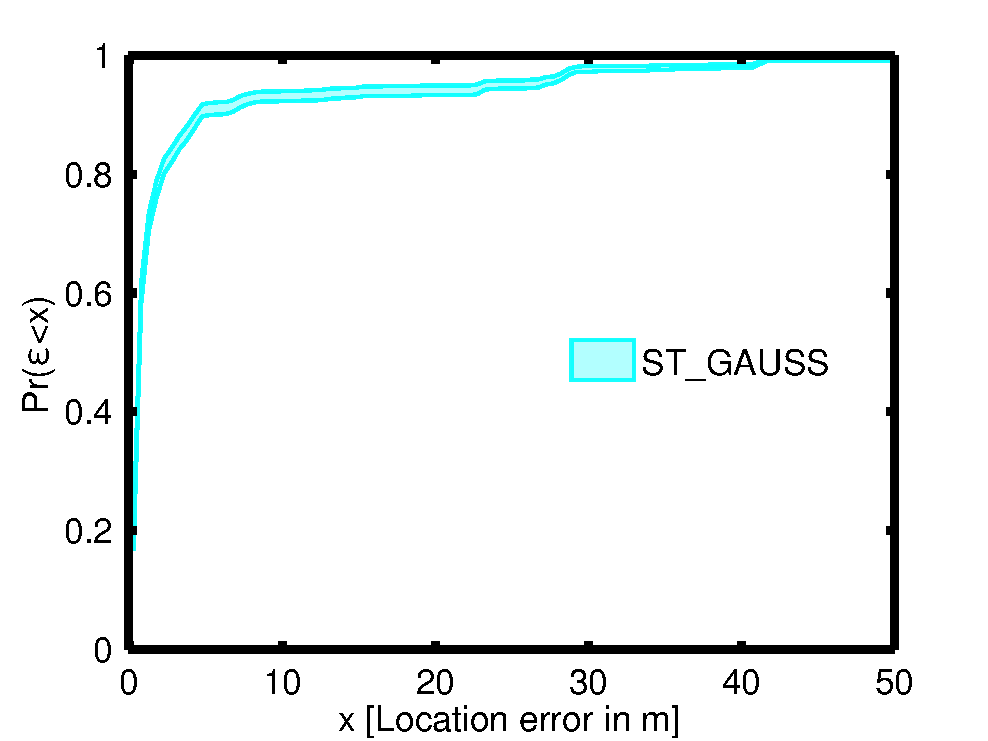
\includegraphics[width=\textwidth]{./gfx/Chapter04/CDF_Figs/ST_GAUSS.pdf}\caption{}\label{fig:CDFd}
%\end{subfigure}
%
%\begin{subfigure}[b]{\linewidth}
%
%	\begin{subfigure}[b]{.45\linewidth}
%	\centering
%	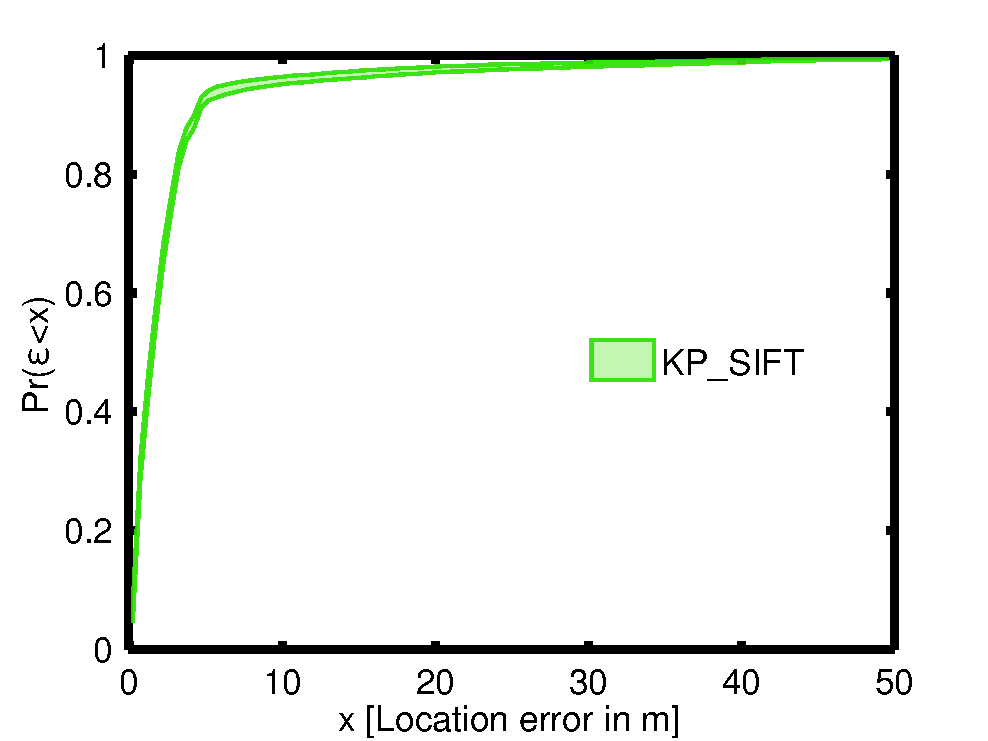
\includegraphics[width=\textwidth]{./gfx/Chapter04/CDF_Figs/KPSIFT.pdf}\caption{}\label{fig:CDFe}
%	\end{subfigure}
%	\begin{subfigure}[b]{.45\linewidth}
%	\centering
%	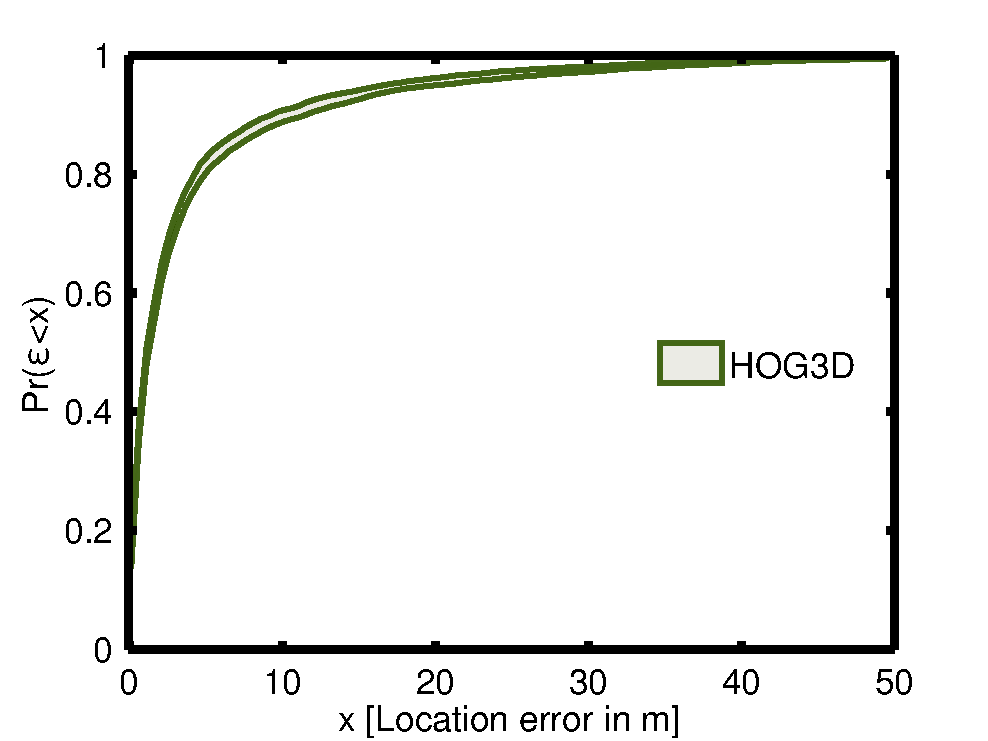
\includegraphics[width=\textwidth]{./gfx/Chapter04/CDF_Figs/HOG3D.pdf}\caption{}\label{fig:CDFf}
%	\end{subfigure}
%	
%\end{subfigure}
%
%\end{subfigure}
%
%\end{subfigure}%
%\begin{subfigure}[b]{.4\linewidth}
%\centering
%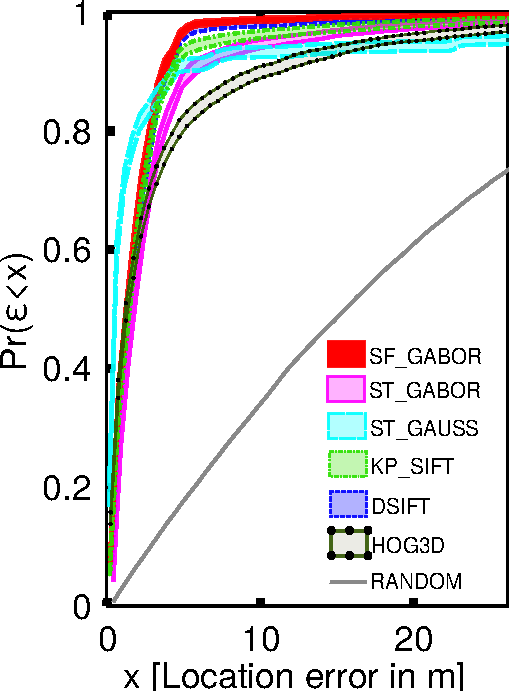
\includegraphics[width=0.95\textwidth]{./gfx/Chapter04/CDF_Figs/CDF_all.pdf}\caption{Comparison between the error distribution obtained with the different methods. The results for a random test (RANDOM) were introduced as a ``sanity check''.}\label{fig:CDFglobal}\label{fig:CDFall}
%\end{subfigure}%
%\caption{Cumulative Distribution Functions of the methods under study.}
%\end{center}
%\end{figure}

\subsection{Localisation error vs ground-truth route positions}

As described in the previous section, by permuting the database paths and selecting, randomly, queries from the remaining path that was left out in the dictionary creation, one can assess the errors  in localisation along each corridor for each pass, and calculate, also, the average error in localisation on a per-corridor basis, or per-path basis.  For these, the ground-truth information acquired as described in Section \ref{sec:Dataset} was used.  Figure~\ref{fig:x_e_vs_gt} provides some examples of the nature of the errors, showing evidence of those locations that are often confused with each other.  As can be seen, for the better method (top trace of Figure~\ref{fig:x_e_vs_gt}) whilst average errors might be small, there are, occasionally, large errors due to poor matching (middle trace). Errors are significantly worse for queries between different devices (see Figure~\ref{fig:x_e_vs_gt}(c)). 

\begin{figure}[h!]
\centering
\subfloat[Corridor 3 using Pass 2 acquired with LG Nexus 4. Results for the best spatio-temporal method, ST-GABOR.]{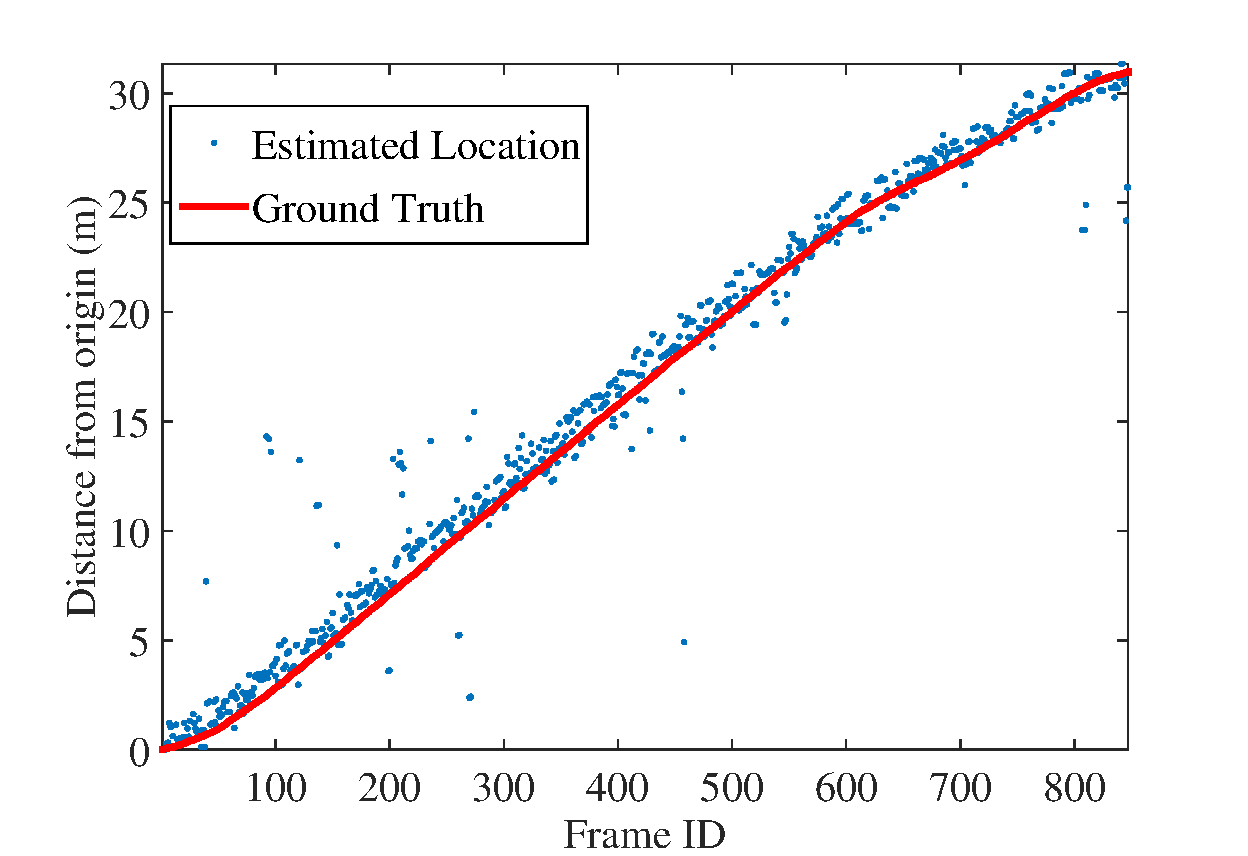
\includegraphics[width=.6\linewidth]{./gfx/Chapter04/xe_vs_x/ST_GABOR_good.pdf}}
\\
\subfloat[Corridor 3 using Pass 6 acquired with Google Glass. Results for the best single-frame method, SF-GABOR.]{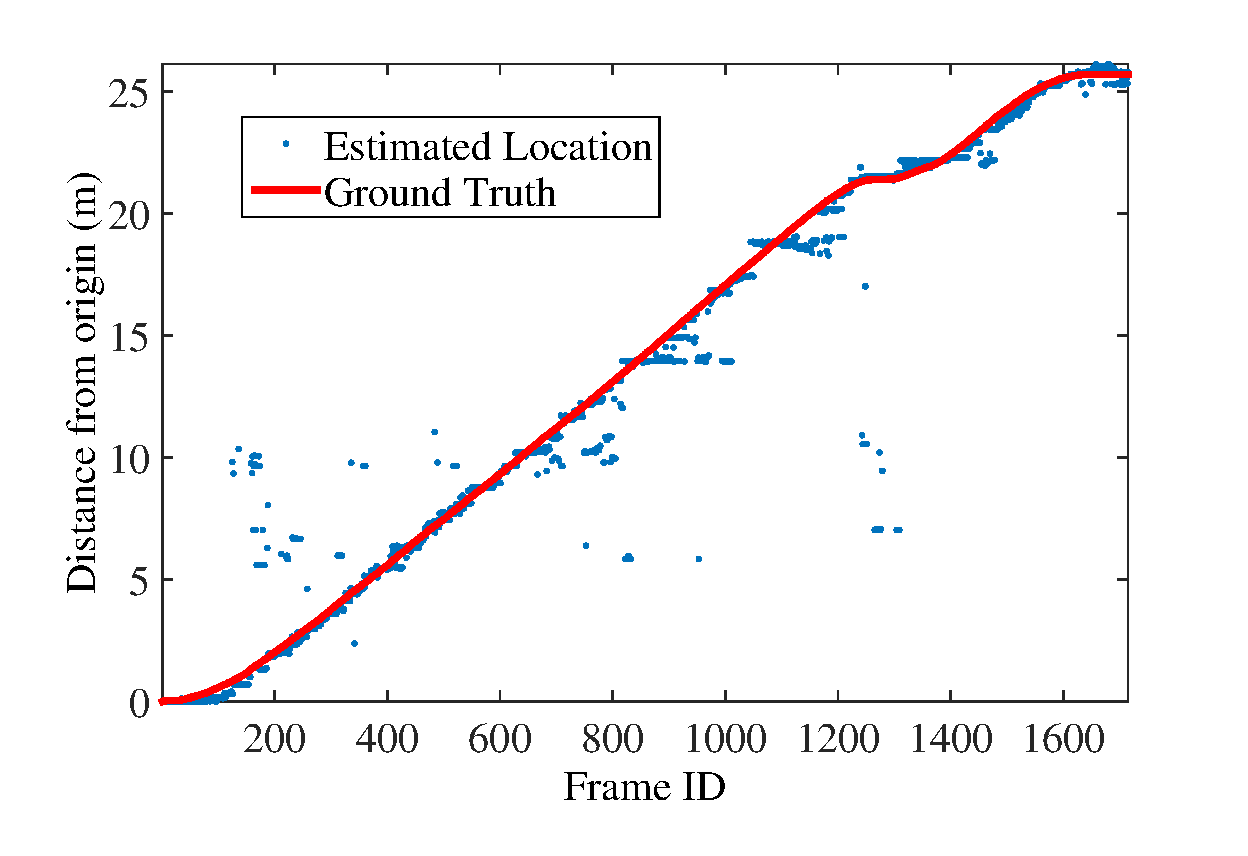
\includegraphics[width=.6\linewidth]{./gfx/Chapter04/xe_vs_x/SF_GABOR_good.pdf}}
\\
\subfloat[Corridor 2 using Pass 6 acquired with Google Glass. Results for the worst overall method, LW-COLOR.]{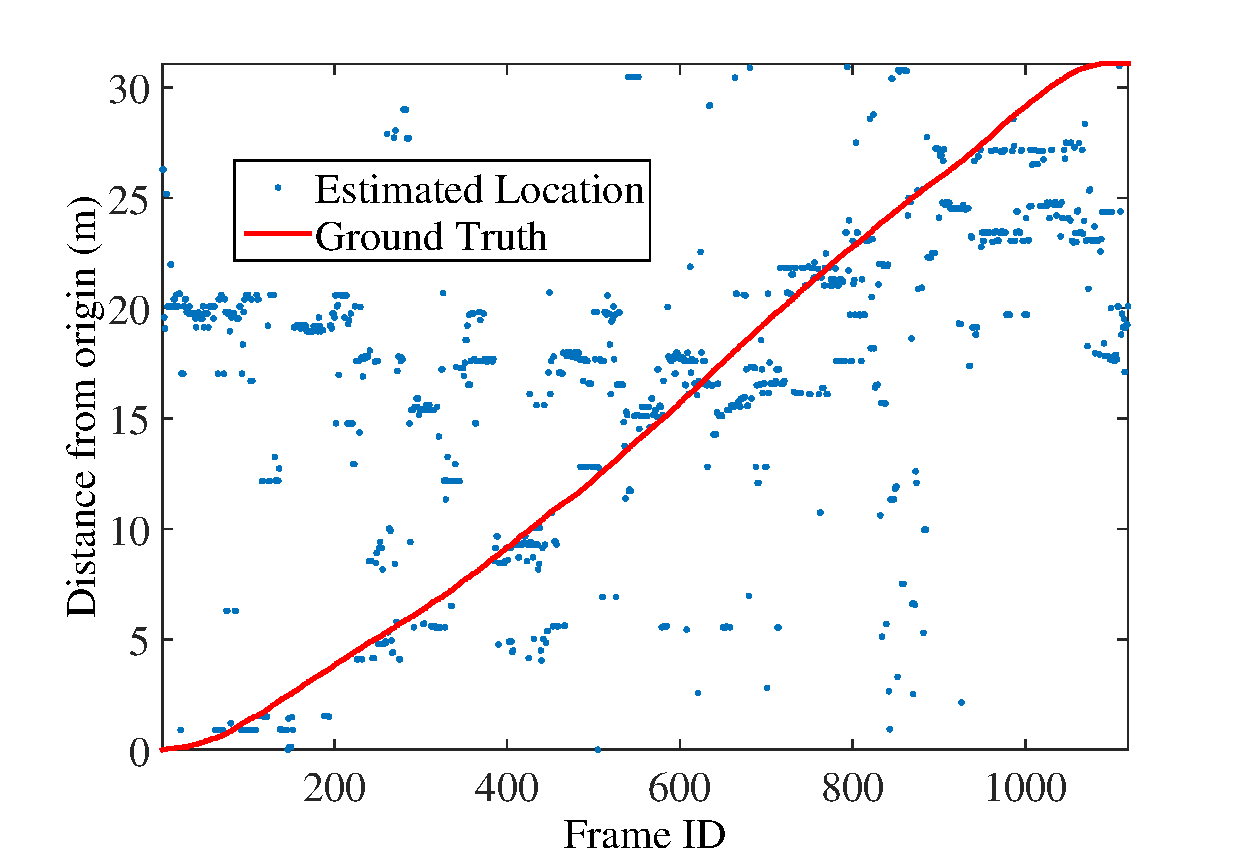
\includegraphics[width=.6\linewidth]{./gfx/Chapter04/xe_vs_x/Lightweight_bad.pdf}}
\caption{Estimated location vs. ground truth. Illustrative examples of good/bad location estimation performance. a) Uses the best descriptor and a single-device dataset, b) uses the best descriptor and a cross-device dataset and c) uses the worst descriptor, and a multiple-device dataset.}
\label{fig:x_e_vs_gt}
\end{figure}


\subsection{Performance Summaries}
\label{visloc_perf}
I calculated the average of the absolute positional error (in m) and the standard deviation of the absolute positional error in a subset of the complete RSM dataset (Table~\ref{Table:summaries}). I  used a leave-one-journey-out approach (all the frames from an entire journey are excluded from the database).  Also using bootstrap sampling, I also estimated the cumulative density functions of the error distributions in position, which are plotted separately in Figure \ref{fig:CDFglobal} and in the same graph in Figure~\ref{fig:CDFall}. The variability in these curves is shown, although it is hard to appreciate. It has been therefore summarised in the last two columns of Table~\ref{Table:summaries} through the area-under-curve (AUC) values. In the best case (SF-GABOR), AUCs of the order of $~96\%$ would mean errors generally below 2 m; in the worst (HOG3D), AUCs $\approx$ 90\% would mean errors of around 5 m.  These  mean absolute error estimates are obtained as the queries, the dictionary and the paths in the database are permuted. 


\begin{table}[!h]
\centering

    \begin{tabular}{ c c c c c }
    \hline
  %  Method   &  Encoding & $\mu_{\epsilon}$ &  $\sigma_{\epsilon}$  & min AUC & max AUC \\ \hline
     \multirow{2}{*}{\bf Method}  & \multicolumn{2}{c}{Error summary (\SI{}{m})} & \multicolumn{2}{c}{AUC (\%)}\\ \cline{2-5}    
    & $\mu_{\epsilon}$ & $\sigma_{\epsilon}$ & Min & Max \\ \hline

    SF-GABOR       & \textbf{1.59}             & 0.11             & 96.11   & \textbf{96.39}   \\ \hline
    %SF-GABOR & Hellinger      & 135.1              & 46.5              & 96.29   & 96.71   \\ \hline
	DSIFT           & 1.62              & 0.11  & 95.96   & 96.31   \\ \hline 

	KP-SIFT           & 2.14              & 0.17  & 94.58   & 95.19   \\ \hline 

	LW-COLOR           & 3.64              & 1.13  & 91.42   & 92.25   \\ \hline \hline

    %SIFT     & Hellinger      & 132.7              & 41.4              & 94.34   & 94.95   \\ \hline

	% Spatio temporal
	
	ST-GAUSS        & \textbf{2.11}              & 0.24 & 94.82   & \textbf{95.57}   \\ \hline
    %ST-GAUSS & Hellinger      & 144.1              & 52.4              & 92.69   & 93.47   \\ \hline
    ST-GABOR       & 2.54              & 0.19 & 93.90   & 94.44   \\ \hline
    %ST-GABOR & Hellinger      & 179.5              & 62.3              & 93.98   & 94.60   \\ \hline

    HOG3D         & 4.20              & 1.33              & 90.89   & 91.83   \\ \hline
    %HOG3D    & Hellinger      & 366.5              & 120.3              & 91.49   & 92.37   \\ \hline
    %LW-COLOR & N/A       & 363.9              & 113.2              & 91.42   & 92.25   \\ \hline
    \end{tabular}


\caption{Summaries of average absolute positional error and standard deviation of positional errors for different descriptor types. $\mu_{\epsilon}$ is the average absolute error, and $\sigma_{\epsilon}$ is the standard deviation of the error in metres. Top: single-frame methods. Bottom: spatio-temporal methods.}
\label{Table:summaries}
\end{table}

Note that tracking algorithms were not used, and so there is no motion model or estimate of current location given the previous one. As it will be described in Section \ref{sec:slamcomp}, incorporating a particle filter or Kalman filter should reduce the errors, particularly where there are large jumps within small intervals of time. This deliberate choice allows us to evaluate the performance of different descriptor and metric choices independently.

The results show that localisation is achieved with good accuracy in terms of CDF and AUC without a large difference between the applied methods, despite the big diversity in their complexity. Absolute errors show significant differences between methods, with average absolute errors in the range of \SI{1.5}{m} to \SI{4.20}{m}. Single-frame methods (SF-GABOR, KP-SIFT and DSIFT) perform slightly better than spatio-temporal approaches (LW-COLOR, ST-GABOR, ST-GAUSS and HOG3D). This is not surprising, as the spatio-temporal methods might be strongly affected by the self motion over fine temporal scales.

In spite of using image retrieval methods in isolation, the attainable accuracy appears to be in line with those of  other methods reviewed in Section~\ref{sec:retrieval}.  However, previously reported methods include tracking, the use of other sensors, or estimates of motion. In this work, I emphasise that no form of tracking was used in estimating position: this was deliberate, in order to assess performance in inferring location from the visual data fairly.  Introducing tracking would probably improve localisation performance, and could reduce query complexity. Yet, tracking often relies on some form of motion model, and for pedestrians carrying or wearing cameras, motion can sometimes be relatively unpredictable. In the next section I will describe the comparison of the appearance-based approaches with SLAM methods, particularly through comparing performance with large-scale direct monocular SLAM (LSD-SLAM).

%------------------------------------------------------------------------- 
\section{Comparison with SLAM}
\label{sec:slamcomp}


\subsection{Description of the experiments}

The first attempt to put the appearance-based approaches into perspective consisted of applying one implementation of the simultaneous localisation and mapping technique (SLAM) to the RSM dataset, at the same frame resolution as for the appearance-based  localisation discussed in this chapter. I chose the ``EKF Mono SLAM'' \citep{civera20091}, which uses an extended Kalman filter (EKF) with 1-point RANSAC.  This implementation was selected for three reasons: a) it is a monocular SLAM technique, so comparison with the single-camera approach is fairer; b) the authors of this package report error estimates -- in the form of error distributions; and c) the errors from video with similar resolutions (240 $\times$ 320) to the small images (208 $\times$ 117) used for the appearance-based matching were reported as being below 2 m for some sequences \citep{civera20091} in their dataset.

The results of the comparison were surprising, and somewhat unsatisfactory. The challenging ambiguity of the sequences in the RSM dataset, and possibly the low resolution of the queries, might explain the results. The feature detector, a FAST corner detector \citep{rosten2006machine}, produced a small number of features in its original  configuration. I lowered the feature detection threshold until the system worked on a small number of frames from each sequence. Even with more permissive thresholds, the average number of FAST features averaged only 20 across the experiments of the RSM dataset. This small number of features led to inaccuracy in the position estimates, causing many of the experimental runs to stop when no features could be matched. The small number of features per frame is also not comparable with the feature density of the methods described in this work, where an average of 2,000 features per frame was obtained for the ``dense'' approaches. Dense SLAM algorithms might fare better, and that was the reason why LSD-SLAM was chosen, as I will describe in the next section.

\subsubsection{Comparison with state-of-the-art SLAM: LSD-SLAM}
\label{sec:comparisonSLAM}

I compared the best performing appearance-based method, SF-GABOR, against the current state-of-the-art in SLAM for indoor sequences, LSD-SLAM.  I first ran the LSD-SLAM code over the 60 video sequences of the RSM dataset and retrieved the results from the visual odometry engine in order to obtain position estimates for each processed frame.  This provided an estimate of the distance travelled by a user, allowing comparison to the results for the appearance-based method. 

The cameras in the devices used to acquire the RSM data are quite different for those suggested for use with LSD-SLAM (recommended: monochrome global-shutter camera with fish eye lens); therefore, the standard LSD-SLAM software was modified to recover from lost tracking when this happened. The semi-dense SLAM parameters were adjusted to adapt best to our conditions and data, specifically, to minimise instances of lost tracking in medium resolution versions ($1024 \times 576$) of the images, i.e. at a considerably higher resolution than the image required for the appearance-based approach. In \ref{sec:slampars} I provide the parameter values that were used for the experiments.


\subsubsection{Performance of LSD-SLAM on RSM dataset sequences}

Figure~\ref{fig:slamperfA} and \ref{fig:slamperfB} illustrate the localisation performance of LSD-SLAM (blue) with respect to the ground truth (red). The two cases that are shown were selected to illustrate that accuracy of localisation can vary, depending on the specific corridor within the RSM dataset (see Section~\ref{sec:Dataset}). As can be seen from the figures, in the better case, the absolute error is below \SI{2}{\metre}. However, in some cases, errors rise as high as $5$ m. Perhaps equally importantly, these errors were found when operating at image sizes that allowed LSD-SLAM to function without losing tracking.

\begin{figure}
	\centering
	\subfloat[(a)][Errors obtained from one experiment using LSD-SLAM. The maximum absolute error was just over $1$ m. ]{
	\setlength\figureheight{0.5\textwidth}	
	\setlength\figurewidth{0.8\textwidth}
	% This file was created by matlab2tikz.
% Minimal pgfplots version: 1.3
%
%The latest updates can be retrieved from
%  http://www.mathworks.com/matlabcentral/fileexchange/22022-matlab2tikz
%where you can also make suggestions and rate matlab2tikz.
%
\definecolor{mycolor1}{rgb}{0.00000,0.44700,0.74100}%
\definecolor{mycolor2}{rgb}{0.85000,0.32500,0.09800}%
\definecolor{mycolor3}{rgb}{0.92900,0.69400,0.12500}%
%
\begin{tikzpicture}

\begin{axis}[%
width=0.95092\figurewidth,
height=\figureheight,
at={(0\figurewidth,0\figureheight)},
scale only axis,
xmin=1,
xmax=1314,
xlabel={Frame index},
/pgf/number format/1000 sep={},
ymin=0,
ymax=3792.5,
yticklabels={0,5,10,15,20,25,30,35},
ylabel={Distance along the path (m)},
legend style={at={(0.178988,0.704846)},anchor=south west,legend cell align=left,align=left,draw=white!15!black}
]
\addplot [color=mycolor1,mark size=1.3pt,only marks,mark=*,mark options={solid}]
  table[row sep=crcr]{%
1	170.29\\
2	171.43\\
3	172.57\\
4	173.71\\
5	174.86\\
6	176\\
7	177.14\\
8	178.29\\
9	179.43\\
10	180.57\\
11	181.71\\
12	182.86\\
13	184\\
14	185.14\\
15	186.29\\
16	187.43\\
17	188.57\\
18	189.71\\
19	190.86\\
20	192\\
21	193.14\\
22	194.29\\
23	195.43\\
24	196.57\\
25	197.71\\
26	198.86\\
27	200\\
28	201.14\\
29	202.29\\
30	203.43\\
31	204.57\\
32	205.71\\
33	206.86\\
34	208\\
35	209.14\\
36	210.29\\
37	211.43\\
38	212.57\\
39	213.71\\
40	214.86\\
41	216\\
42	217.14\\
43	218.29\\
44	219.43\\
45	220.57\\
46	221.71\\
47	222.86\\
48	224\\
49	225.14\\
50	226.29\\
51	227.43\\
52	228.57\\
53	229.71\\
54	230.86\\
55	232\\
56	233.14\\
57	234.29\\
58	235.43\\
59	236.57\\
60	237.71\\
61	238.86\\
62	240\\
63	244.86\\
64	249.71\\
65	254.57\\
66	259.43\\
67	264.29\\
68	269.14\\
69	274\\
70	278.86\\
71	283.71\\
72	288.57\\
73	293.43\\
74	298.29\\
75	303.14\\
76	308\\
77	312.86\\
78	317.71\\
79	322.57\\
80	327.43\\
81	332.29\\
82	337.14\\
83	342\\
84	346.86\\
85	351.71\\
86	356.57\\
87	361.43\\
88	366.29\\
89	371.14\\
90	376\\
91	380.86\\
92	385.71\\
93	390.57\\
94	395.43\\
95	400.29\\
96	405.14\\
97	410\\
98	414.86\\
99	419.71\\
100	424.57\\
101	429.43\\
102	434.29\\
103	439.14\\
104	444\\
105	448.86\\
106	453.71\\
107	458.57\\
108	463.43\\
109	468.29\\
110	473.14\\
111	478\\
112	482.86\\
113	487.71\\
114	492.57\\
115	497.43\\
116	502.29\\
117	507.14\\
118	512\\
119	516.86\\
120	521.71\\
121	526.57\\
122	531.43\\
123	536.29\\
124	541.14\\
125	546\\
126	550.86\\
127	555.71\\
128	560.57\\
129	565.43\\
130	570.29\\
131	575.14\\
132	580\\
133	582.4\\
134	584.8\\
135	587.2\\
136	589.6\\
137	592\\
138	594.4\\
139	596.8\\
140	599.2\\
141	601.6\\
142	604\\
143	606.4\\
144	608.8\\
145	611.2\\
146	613.6\\
147	616\\
148	618.4\\
149	620.8\\
150	623.2\\
151	625.6\\
152	628\\
153	630.4\\
154	632.8\\
155	635.2\\
156	637.6\\
157	640\\
158	642.4\\
159	644.8\\
160	647.2\\
161	649.6\\
162	652\\
163	654.4\\
164	656.8\\
165	659.2\\
166	661.6\\
167	664\\
168	666.4\\
169	668.8\\
170	671.2\\
171	673.6\\
172	676\\
173	678.4\\
174	680.8\\
175	683.2\\
176	685.6\\
177	688\\
178	690.4\\
179	692.8\\
180	695.2\\
181	697.6\\
182	700\\
183	702.4\\
184	704.8\\
185	707.2\\
186	709.6\\
187	712\\
188	714.4\\
189	716.8\\
190	719.2\\
191	721.6\\
192	724\\
193	726.4\\
194	728.8\\
195	731.2\\
196	733.6\\
197	736\\
198	738.4\\
199	740.8\\
200	743.2\\
201	745.6\\
202	748\\
203	750.4\\
204	752.8\\
205	755.2\\
206	757.6\\
207	760\\
208	762.4\\
209	764.8\\
210	767.2\\
211	769.6\\
212	772\\
213	774.4\\
214	776.8\\
215	779.2\\
216	781.6\\
217	784\\
218	786.4\\
219	788.8\\
220	791.2\\
221	793.6\\
222	796\\
223	798.4\\
224	800.8\\
225	803.2\\
226	805.6\\
227	808\\
228	810.4\\
229	812.8\\
230	815.2\\
231	817.6\\
232	820\\
233	822.64\\
234	825.27\\
235	827.91\\
236	830.55\\
237	833.18\\
238	835.82\\
239	838.45\\
240	841.09\\
241	843.73\\
242	846.36\\
243	849\\
244	851.64\\
245	854.27\\
246	856.91\\
247	859.55\\
248	862.18\\
249	864.82\\
250	867.45\\
251	870.09\\
252	872.73\\
253	875.36\\
254	878\\
255	880.64\\
256	883.27\\
257	885.91\\
258	888.55\\
259	891.18\\
260	893.82\\
261	896.45\\
262	899.09\\
263	901.73\\
264	904.36\\
265	907\\
266	909.64\\
267	912.27\\
268	914.91\\
269	917.55\\
270	920.18\\
271	922.82\\
272	925.45\\
273	928.09\\
274	930.73\\
275	933.36\\
276	936\\
277	938.64\\
278	941.27\\
279	943.91\\
280	946.55\\
281	949.18\\
282	951.82\\
283	954.45\\
284	957.09\\
285	959.73\\
286	962.36\\
287	965\\
288	967.64\\
289	970.27\\
290	972.91\\
291	975.55\\
292	978.18\\
293	980.82\\
294	983.45\\
295	986.09\\
296	988.73\\
297	991.36\\
298	994\\
299	996.64\\
300	999.27\\
301	1001.91\\
302	1004.55\\
303	1007.18\\
304	1009.82\\
305	1012.45\\
306	1015.09\\
307	1017.73\\
308	1020.36\\
309	1023\\
310	1025.64\\
311	1028.27\\
312	1030.91\\
313	1033.55\\
314	1036.18\\
315	1038.82\\
316	1041.45\\
317	1044.09\\
318	1046.73\\
319	1049.36\\
320	1052\\
321	1054.64\\
322	1057.27\\
323	1059.91\\
324	1062.55\\
325	1065.18\\
326	1067.82\\
327	1070.45\\
328	1073.09\\
329	1075.73\\
330	1078.36\\
331	1081\\
332	1083.64\\
333	1086.27\\
334	1088.91\\
335	1091.55\\
336	1094.18\\
337	1096.82\\
338	1099.45\\
339	1102.09\\
340	1104.73\\
341	1107.36\\
342	1110\\
343	1111.19\\
344	1112.38\\
345	1113.56\\
346	1114.75\\
347	1115.94\\
348	1117.12\\
349	1118.31\\
350	1119.5\\
351	1120.69\\
352	1121.88\\
353	1123.06\\
354	1124.25\\
355	1125.44\\
356	1126.62\\
357	1127.81\\
358	1129\\
359	1130.19\\
360	1131.38\\
361	1132.56\\
362	1133.75\\
363	1134.94\\
364	1136.12\\
365	1137.31\\
366	1138.5\\
367	1139.69\\
368	1140.88\\
369	1142.06\\
370	1143.25\\
371	1144.44\\
372	1145.62\\
373	1146.81\\
374	1148\\
375	1149.19\\
376	1150.38\\
377	1151.56\\
378	1152.75\\
379	1153.94\\
380	1155.12\\
381	1156.31\\
382	1157.5\\
383	1158.69\\
384	1159.88\\
385	1161.06\\
386	1162.25\\
387	1163.44\\
388	1164.62\\
389	1165.81\\
390	1167\\
391	1168.19\\
392	1169.38\\
393	1170.56\\
394	1171.75\\
395	1172.94\\
396	1174.12\\
397	1175.31\\
398	1176.5\\
399	1177.69\\
400	1178.88\\
401	1180.06\\
402	1181.25\\
403	1182.44\\
404	1183.62\\
405	1184.81\\
406	1186\\
407	1187.19\\
408	1188.38\\
409	1189.56\\
410	1190.75\\
411	1191.94\\
412	1193.12\\
413	1194.31\\
414	1195.5\\
415	1196.69\\
416	1197.88\\
417	1199.06\\
418	1200.25\\
419	1201.44\\
420	1202.62\\
421	1203.81\\
422	1205\\
423	1206.19\\
424	1207.38\\
425	1208.56\\
426	1209.75\\
427	1210.94\\
428	1212.12\\
429	1213.31\\
430	1214.5\\
431	1215.69\\
432	1216.88\\
433	1218.06\\
434	1219.25\\
435	1220.44\\
436	1221.62\\
437	1222.81\\
438	1224\\
439	1225.19\\
440	1226.38\\
441	1227.56\\
442	1228.75\\
443	1229.94\\
444	1231.12\\
445	1232.31\\
446	1233.5\\
447	1234.69\\
448	1235.88\\
449	1237.06\\
450	1238.25\\
451	1239.44\\
452	1240.62\\
453	1241.81\\
454	1243\\
455	1244.19\\
456	1245.38\\
457	1246.56\\
458	1247.75\\
459	1248.94\\
460	1250.12\\
461	1251.31\\
462	1252.5\\
463	1253.69\\
464	1254.88\\
465	1256.06\\
466	1257.25\\
467	1258.44\\
468	1259.62\\
469	1260.81\\
470	1262\\
471	1263.19\\
472	1264.38\\
473	1265.56\\
474	1266.75\\
475	1267.94\\
476	1269.12\\
477	1270.31\\
478	1271.5\\
479	1272.69\\
480	1273.88\\
481	1275.06\\
482	1276.25\\
483	1277.44\\
484	1278.62\\
485	1279.81\\
486	1281\\
487	1282.19\\
488	1283.38\\
489	1284.56\\
490	1285.75\\
491	1286.94\\
492	1288.12\\
493	1289.31\\
494	1290.5\\
495	1291.69\\
496	1292.88\\
497	1294.06\\
498	1295.25\\
499	1296.44\\
500	1297.62\\
501	1298.81\\
502	1300\\
503	1305.75\\
504	1311.5\\
505	1317.25\\
506	1323\\
507	1328.75\\
508	1334.5\\
509	1340.25\\
510	1346\\
511	1351.75\\
512	1357.5\\
513	1363.25\\
514	1369\\
515	1374.75\\
516	1380.5\\
517	1386.25\\
518	1392\\
519	1397.75\\
520	1403.5\\
521	1409.25\\
522	1415\\
523	1420.75\\
524	1426.5\\
525	1432.25\\
526	1438\\
527	1443.75\\
528	1449.5\\
529	1455.25\\
530	1461\\
531	1466.75\\
532	1472.5\\
533	1478.25\\
534	1484\\
535	1489.75\\
536	1495.5\\
537	1501.25\\
538	1507\\
539	1512.75\\
540	1518.5\\
541	1524.25\\
542	1530\\
543	1532.71\\
544	1535.43\\
545	1538.14\\
546	1540.86\\
547	1543.57\\
548	1546.29\\
549	1549\\
550	1551.71\\
551	1554.43\\
552	1557.14\\
553	1559.86\\
554	1562.57\\
555	1565.29\\
556	1568\\
557	1570.71\\
558	1573.43\\
559	1576.14\\
560	1578.86\\
561	1581.57\\
562	1584.29\\
563	1587\\
564	1589.71\\
565	1592.43\\
566	1595.14\\
567	1597.86\\
568	1600.57\\
569	1603.29\\
570	1606\\
571	1608.71\\
572	1611.43\\
573	1614.14\\
574	1616.86\\
575	1619.57\\
576	1622.29\\
577	1625\\
578	1627.71\\
579	1630.43\\
580	1633.14\\
581	1635.86\\
582	1638.57\\
583	1641.29\\
584	1644\\
585	1646.71\\
586	1649.43\\
587	1652.14\\
588	1654.86\\
589	1657.57\\
590	1660.29\\
591	1663\\
592	1665.71\\
593	1668.43\\
594	1671.14\\
595	1673.86\\
596	1676.57\\
597	1679.29\\
598	1682\\
599	1684.71\\
600	1687.43\\
601	1690.14\\
602	1692.86\\
603	1695.57\\
604	1698.29\\
605	1701\\
606	1703.71\\
607	1706.43\\
608	1709.14\\
609	1711.86\\
610	1714.57\\
611	1717.29\\
612	1720\\
613	1722.71\\
614	1725.43\\
615	1728.14\\
616	1730.86\\
617	1733.57\\
618	1736.29\\
619	1739\\
620	1741.71\\
621	1744.43\\
622	1747.14\\
623	1749.86\\
624	1752.57\\
625	1755.29\\
626	1758\\
627	1760.71\\
628	1763.43\\
629	1766.14\\
630	1768.86\\
631	1771.57\\
632	1774.29\\
633	1777\\
634	1779.71\\
635	1782.43\\
636	1785.14\\
637	1787.86\\
638	1790.57\\
639	1793.29\\
640	1796\\
641	1798.71\\
642	1801.43\\
643	1804.14\\
644	1806.86\\
645	1809.57\\
646	1812.29\\
647	1815\\
648	1817.71\\
649	1820.43\\
650	1823.14\\
651	1825.86\\
652	1828.57\\
653	1831.29\\
654	1834\\
655	1836.71\\
656	1839.43\\
657	1842.14\\
658	1844.86\\
659	1847.57\\
660	1850.29\\
661	1853\\
662	1855.71\\
663	1858.43\\
664	1861.14\\
665	1863.86\\
666	1866.57\\
667	1869.29\\
668	1872\\
669	1874.71\\
670	1877.43\\
671	1880.14\\
672	1882.86\\
673	1885.57\\
674	1888.29\\
675	1891\\
676	1893.71\\
677	1896.43\\
678	1899.14\\
679	1901.86\\
680	1904.57\\
681	1907.29\\
682	1910\\
683	1912.75\\
684	1915.5\\
685	1918.25\\
686	1921\\
687	1923.75\\
688	1926.5\\
689	1929.25\\
690	1932\\
691	1934.75\\
692	1937.5\\
693	1940.25\\
694	1943\\
695	1945.75\\
696	1948.5\\
697	1951.25\\
698	1954\\
699	1956.75\\
700	1959.5\\
701	1962.25\\
702	1965\\
703	1967.75\\
704	1970.5\\
705	1973.25\\
706	1976\\
707	1978.75\\
708	1981.5\\
709	1984.25\\
710	1987\\
711	1989.75\\
712	1992.5\\
713	1995.25\\
714	1998\\
715	2000.75\\
716	2003.5\\
717	2006.25\\
718	2009\\
719	2011.75\\
720	2014.5\\
721	2017.25\\
722	2020\\
723	2022.75\\
724	2025.5\\
725	2028.25\\
726	2031\\
727	2033.75\\
728	2036.5\\
729	2039.25\\
730	2042\\
731	2044.75\\
732	2047.5\\
733	2050.25\\
734	2053\\
735	2055.75\\
736	2058.5\\
737	2061.25\\
738	2064\\
739	2066.75\\
740	2069.5\\
741	2072.25\\
742	2075\\
743	2077.75\\
744	2080.5\\
745	2083.25\\
746	2086\\
747	2088.75\\
748	2091.5\\
749	2094.25\\
750	2097\\
751	2099.75\\
752	2102.5\\
753	2105.25\\
754	2108\\
755	2110.75\\
756	2113.5\\
757	2116.25\\
758	2119\\
759	2121.75\\
760	2124.5\\
761	2127.25\\
762	2130\\
763	2132.57\\
764	2135.14\\
765	2137.71\\
766	2140.29\\
767	2142.86\\
768	2145.43\\
769	2148\\
770	2150.57\\
771	2153.14\\
772	2155.71\\
773	2158.29\\
774	2160.86\\
775	2163.43\\
776	2166\\
777	2168.57\\
778	2171.14\\
779	2173.71\\
780	2176.29\\
781	2178.86\\
782	2181.43\\
783	2184\\
784	2186.57\\
785	2189.14\\
786	2191.71\\
787	2194.29\\
788	2196.86\\
789	2199.43\\
790	2202\\
791	2204.57\\
792	2207.14\\
793	2209.71\\
794	2212.29\\
795	2214.86\\
796	2217.43\\
797	2220\\
798	2222.57\\
799	2225.14\\
800	2227.71\\
801	2230.29\\
802	2232.86\\
803	2235.43\\
804	2238\\
805	2240.57\\
806	2243.14\\
807	2245.71\\
808	2248.29\\
809	2250.86\\
810	2253.43\\
811	2256\\
812	2258.57\\
813	2261.14\\
814	2263.71\\
815	2266.29\\
816	2268.86\\
817	2271.43\\
818	2274\\
819	2276.57\\
820	2279.14\\
821	2281.71\\
822	2284.29\\
823	2286.86\\
824	2289.43\\
825	2292\\
826	2294.57\\
827	2297.14\\
828	2299.71\\
829	2302.29\\
830	2304.86\\
831	2307.43\\
832	2310\\
833	2313.33\\
834	2316.67\\
835	2320\\
836	2323.33\\
837	2326.67\\
838	2330\\
839	2333.33\\
840	2336.67\\
841	2340\\
842	2343.33\\
843	2346.67\\
844	2350\\
845	2353.33\\
846	2356.67\\
847	2360\\
848	2363.33\\
849	2366.67\\
850	2370\\
851	2373.33\\
852	2376.67\\
853	2380\\
854	2383.33\\
855	2386.67\\
856	2390\\
857	2393.33\\
858	2396.67\\
859	2400\\
860	2403.33\\
861	2406.67\\
862	2410\\
863	2413.33\\
864	2416.67\\
865	2420\\
866	2423.33\\
867	2426.67\\
868	2430\\
869	2433.33\\
870	2436.67\\
871	2440\\
872	2443.33\\
873	2446.67\\
874	2450\\
875	2453.33\\
876	2456.67\\
877	2460\\
878	2463.33\\
879	2466.67\\
880	2470\\
881	2473.33\\
882	2476.67\\
883	2480\\
884	2483.33\\
885	2486.67\\
886	2490\\
887	2493.33\\
888	2496.67\\
889	2500\\
890	2503.33\\
891	2506.67\\
892	2510\\
893	2512.92\\
894	2515.83\\
895	2518.75\\
896	2521.67\\
897	2524.58\\
898	2527.5\\
899	2530.42\\
900	2533.33\\
901	2536.25\\
902	2539.17\\
903	2542.08\\
904	2545\\
905	2547.92\\
906	2550.83\\
907	2553.75\\
908	2556.67\\
909	2559.58\\
910	2562.5\\
911	2565.42\\
912	2568.33\\
913	2571.25\\
914	2574.17\\
915	2577.08\\
916	2580\\
917	2582.92\\
918	2585.83\\
919	2588.75\\
920	2591.67\\
921	2594.58\\
922	2597.5\\
923	2600.42\\
924	2603.33\\
925	2606.25\\
926	2609.17\\
927	2612.08\\
928	2615\\
929	2617.92\\
930	2620.83\\
931	2623.75\\
932	2626.67\\
933	2629.58\\
934	2632.5\\
935	2635.42\\
936	2638.33\\
937	2641.25\\
938	2644.17\\
939	2647.08\\
940	2650\\
941	2652.92\\
942	2655.83\\
943	2658.75\\
944	2661.67\\
945	2664.58\\
946	2667.5\\
947	2670.42\\
948	2673.33\\
949	2676.25\\
950	2679.17\\
951	2682.08\\
952	2685\\
953	2687.92\\
954	2690.83\\
955	2693.75\\
956	2696.67\\
957	2699.58\\
958	2702.5\\
959	2705.42\\
960	2708.33\\
961	2711.25\\
962	2714.17\\
963	2717.08\\
964	2720\\
965	2722.92\\
966	2725.83\\
967	2728.75\\
968	2731.67\\
969	2734.58\\
970	2737.5\\
971	2740.42\\
972	2743.33\\
973	2746.25\\
974	2749.17\\
975	2752.08\\
976	2755\\
977	2757.92\\
978	2760.83\\
979	2763.75\\
980	2766.67\\
981	2769.58\\
982	2772.5\\
983	2775.42\\
984	2778.33\\
985	2781.25\\
986	2784.17\\
987	2787.08\\
988	2790\\
989	2792.92\\
990	2795.83\\
991	2798.75\\
992	2801.67\\
993	2804.58\\
994	2807.5\\
995	2810.42\\
996	2813.33\\
997	2816.25\\
998	2819.17\\
999	2822.08\\
1000	2825\\
1001	2827.92\\
1002	2830.83\\
1003	2833.75\\
1004	2836.67\\
1005	2839.58\\
1006	2842.5\\
1007	2845.42\\
1008	2848.33\\
1009	2851.25\\
1010	2854.17\\
1011	2857.08\\
1012	2860\\
1013	2863.38\\
1014	2866.75\\
1015	2870.12\\
1016	2873.5\\
1017	2876.88\\
1018	2880.25\\
1019	2883.62\\
1020	2887\\
1021	2890.38\\
1022	2893.75\\
1023	2897.12\\
1024	2900.5\\
1025	2903.88\\
1026	2907.25\\
1027	2910.62\\
1028	2914\\
1029	2917.38\\
1030	2920.75\\
1031	2924.12\\
1032	2927.5\\
1033	2930.88\\
1034	2934.25\\
1035	2937.62\\
1036	2941\\
1037	2944.38\\
1038	2947.75\\
1039	2951.12\\
1040	2954.5\\
1041	2957.88\\
1042	2961.25\\
1043	2964.62\\
1044	2968\\
1045	2971.38\\
1046	2974.75\\
1047	2978.12\\
1048	2981.5\\
1049	2984.88\\
1050	2988.25\\
1051	2991.62\\
1052	2995\\
1053	2998.38\\
1054	3001.75\\
1055	3005.12\\
1056	3008.5\\
1057	3011.88\\
1058	3015.25\\
1059	3018.62\\
1060	3022\\
1061	3025.38\\
1062	3028.75\\
1063	3032.12\\
1064	3035.5\\
1065	3038.88\\
1066	3042.25\\
1067	3045.62\\
1068	3049\\
1069	3052.38\\
1070	3055.75\\
1071	3059.12\\
1072	3062.5\\
1073	3065.88\\
1074	3069.25\\
1075	3072.62\\
1076	3076\\
1077	3079.38\\
1078	3082.75\\
1079	3086.12\\
1080	3089.5\\
1081	3092.88\\
1082	3096.25\\
1083	3099.62\\
1084	3103\\
1085	3106.38\\
1086	3109.75\\
1087	3113.12\\
1088	3116.5\\
1089	3119.88\\
1090	3123.25\\
1091	3126.62\\
1092	3130\\
1093	3133.64\\
1094	3137.27\\
1095	3140.91\\
1096	3144.55\\
1097	3148.18\\
1098	3151.82\\
1099	3155.45\\
1100	3159.09\\
1101	3162.73\\
1102	3166.36\\
1103	3170\\
1104	3173.64\\
1105	3177.27\\
1106	3180.91\\
1107	3184.55\\
1108	3188.18\\
1109	3191.82\\
1110	3195.45\\
1111	3199.09\\
1112	3202.73\\
1113	3206.36\\
1114	3210\\
1115	3213.64\\
1116	3217.27\\
1117	3220.91\\
1118	3224.55\\
1119	3228.18\\
1120	3231.82\\
1121	3235.45\\
1122	3239.09\\
1123	3242.73\\
1124	3246.36\\
1125	3250\\
1126	3253.64\\
1127	3257.27\\
1128	3260.91\\
1129	3264.55\\
1130	3268.18\\
1131	3271.82\\
1132	3275.45\\
1133	3279.09\\
1134	3282.73\\
1135	3286.36\\
1136	3290\\
1137	3293.64\\
1138	3297.27\\
1139	3300.91\\
1140	3304.55\\
1141	3308.18\\
1142	3311.82\\
1143	3315.45\\
1144	3319.09\\
1145	3322.73\\
1146	3326.36\\
1147	3330\\
1148	3333.64\\
1149	3337.27\\
1150	3340.91\\
1151	3344.55\\
1152	3348.18\\
1153	3351.82\\
1154	3355.45\\
1155	3359.09\\
1156	3362.73\\
1157	3366.36\\
1158	3370\\
1159	3373.64\\
1160	3377.27\\
1161	3380.91\\
1162	3384.55\\
1163	3388.18\\
1164	3391.82\\
1165	3395.45\\
1166	3399.09\\
1167	3402.73\\
1168	3406.36\\
1169	3410\\
1170	3413.64\\
1171	3417.27\\
1172	3420.91\\
1173	3424.55\\
1174	3428.18\\
1175	3431.82\\
1176	3435.45\\
1177	3439.09\\
1178	3442.73\\
1179	3446.36\\
1180	3450\\
1181	3453.64\\
1182	3457.27\\
1183	3460.91\\
1184	3464.55\\
1185	3468.18\\
1186	3471.82\\
1187	3475.45\\
1188	3479.09\\
1189	3482.73\\
1190	3486.36\\
1191	3490\\
1192	3493.64\\
1193	3497.27\\
1194	3500.91\\
1195	3504.55\\
1196	3508.18\\
1197	3511.82\\
1198	3515.45\\
1199	3519.09\\
1200	3522.73\\
1201	3526.36\\
1202	3530\\
1203	3532\\
1204	3534\\
1205	3536\\
1206	3538\\
1207	3540\\
1208	3542\\
1209	3544\\
1210	3546\\
1211	3548\\
1212	3550\\
1213	3552\\
1214	3554\\
1215	3556\\
1216	3558\\
1217	3560\\
1218	3562\\
1219	3564\\
1220	3566\\
1221	3568\\
1222	3570\\
1223	3572\\
1224	3574\\
1225	3576\\
1226	3578\\
1227	3580\\
1228	3582\\
1229	3584\\
1230	3586\\
1231	3588\\
1232	3590\\
1233	3592\\
1234	3594\\
1235	3596\\
1236	3598\\
1237	3600\\
1238	3602\\
1239	3604\\
1240	3606\\
1241	3608\\
1242	3610\\
1243	3612\\
1244	3614\\
1245	3616\\
1246	3618\\
1247	3620\\
1248	3622\\
1249	3624\\
1250	3626\\
1251	3628\\
1252	3630\\
1253	3632\\
1254	3634\\
1255	3636\\
1256	3638\\
1257	3640\\
1258	3642\\
1259	3644\\
1260	3646\\
1261	3648\\
1262	3650\\
1263	3652\\
1264	3654\\
1265	3656\\
1266	3658\\
1267	3660\\
1268	3662\\
1269	3664\\
1270	3666\\
1271	3668\\
1272	3670\\
1273	3672\\
1274	3674\\
1275	3676\\
1276	3678\\
1277	3680\\
1278	3682\\
1279	3684\\
1280	3686\\
1281	3688\\
1282	3690\\
1283	3692\\
1284	3694\\
1285	3696\\
1286	3698\\
1287	3700\\
1288	3702\\
1289	3704\\
1290	3706\\
1291	3708\\
1292	3710\\
1293	3713.75\\
1294	3717.5\\
1295	3721.25\\
1296	3725\\
1297	3728.75\\
1298	3732.5\\
1299	3736.25\\
1300	3740\\
1301	3743.75\\
1302	3747.5\\
1303	3751.25\\
1304	3755\\
1305	3758.75\\
1306	3762.5\\
1307	3766.25\\
1308	3770\\
1309	3773.75\\
1310	3777.5\\
1311	3781.25\\
1312	3785\\
1313	3788.75\\
1314	3792.5\\
};
\addlegendentry{LSD-SLAM};

\addplot [color=mycolor2,mark size=1.3pt,only marks,mark=*,mark options={solid}]
  table[row sep=crcr]{%
1	170.29\\
2	171.873171070446\\
3	173.469518993372\\
4	175.07528023148\\
5	176.691701232069\\
6	178.31768105005\\
7	179.951675109077\\
8	181.593551876718\\
9	183.24418567529\\
10	184.903943052731\\
11	186.572511321923\\
12	188.258792413739\\
13	189.954271376081\\
14	191.658290427945\\
15	193.369703242656\\
16	195.08931899107\\
17	196.814859698946\\
18	198.55105228577\\
19	200.295459602471\\
20	202.057071891369\\
21	203.829153930332\\
22	205.611316173248\\
23	207.403772667081\\
24	209.204604949939\\
25	211.012152321973\\
26	212.832610184923\\
27	214.658436035669\\
28	216.488829918163\\
29	218.323400168258\\
30	220.169959952379\\
31	222.020311220476\\
32	223.87574983364\\
33	225.734442691425\\
34	227.595874565155\\
35	229.463571448799\\
36	231.33229092297\\
37	233.204314644844\\
38	235.080493766262\\
39	236.962906396646\\
40	238.850025834844\\
41	240.739349097747\\
42	242.63327028332\\
43	244.530229178456\\
44	246.432349591776\\
45	248.33676159784\\
46	250.246507795771\\
47	252.160776539793\\
48	254.062710871228\\
49	255.965558768073\\
50	257.87545622642\\
51	259.785547680382\\
52	261.699287710066\\
53	263.617587205729\\
54	265.538607895887\\
55	267.461498839256\\
56	269.388112982228\\
57	271.317004663008\\
58	273.247786815871\\
59	275.180678226262\\
60	277.102582781298\\
61	279.027824838438\\
62	280.95624283965\\
63	282.888500099214\\
64	284.823480913797\\
65	286.762388316857\\
66	288.705369600853\\
67	290.651362699705\\
68	292.601711888435\\
69	294.556386393671\\
70	296.513363353581\\
71	298.472532191031\\
72	300.434573823009\\
73	302.40042482213\\
74	304.369530668668\\
75	306.340178354498\\
76	308.313452142486\\
77	310.290022874851\\
78	312.269652810006\\
79	314.252298747981\\
80	316.238081779672\\
81	318.22707602045\\
82	320.219706720465\\
83	322.215163118885\\
84	324.214448104819\\
85	326.21745473575\\
86	328.222535180592\\
87	330.225912846147\\
88	332.233033908098\\
89	334.244468669412\\
90	336.260154378267\\
91	338.2798611828\\
92	340.303036538879\\
93	342.332407763758\\
94	344.364174353105\\
95	346.399628827703\\
96	348.438426996068\\
97	350.480148617455\\
98	352.525818701743\\
99	354.574704476303\\
100	356.626607659143\\
101	358.680719497849\\
102	360.736704706558\\
103	362.795041358388\\
104	364.857477767174\\
105	366.923072146478\\
106	368.991482644401\\
107	371.062810279771\\
108	373.140564206318\\
109	375.22166530485\\
110	377.306120437638\\
111	379.393243772105\\
112	381.483420313151\\
113	383.57760202196\\
114	385.675423347918\\
115	387.777075673706\\
116	389.883252729968\\
117	391.992554724292\\
118	394.106101891889\\
119	396.224093387848\\
120	398.34648746815\\
121	400.473655288015\\
122	402.605344156013\\
123	404.738364719905\\
124	406.872221765869\\
125	409.013098976366\\
126	411.157661831991\\
127	413.304838389364\\
128	415.454576056582\\
129	417.606852087298\\
130	419.762768525551\\
131	421.921118665223\\
132	424.080988006622\\
133	426.244043694938\\
134	428.410301983146\\
135	430.579106927766\\
136	432.75134690992\\
137	434.926359898574\\
138	437.104630346254\\
139	439.285337233392\\
140	441.469852026951\\
141	443.659027741355\\
142	445.851587170214\\
143	448.047845218284\\
144	450.24737332506\\
145	452.448779622438\\
146	454.65402302363\\
147	456.862445988968\\
148	459.071296940557\\
149	461.283714951579\\
150	463.499354130913\\
151	465.716985018003\\
152	467.937628477028\\
153	470.160829861988\\
154	472.386589730907\\
155	474.615013961157\\
156	476.845686321457\\
157	479.078767177601\\
158	481.313948450026\\
159	483.55128845077\\
160	485.791161360871\\
161	488.033721932482\\
162	490.277146119063\\
163	492.523271360852\\
164	494.772623088064\\
165	497.024763852125\\
166	499.280591686911\\
167	501.538345532611\\
168	503.799191950567\\
169	506.063371925817\\
170	508.330136912202\\
171	510.600235367872\\
172	512.873582026816\\
173	515.15012883713\\
174	517.429604101867\\
175	519.709623352114\\
176	521.991822808564\\
177	524.275489606726\\
178	526.5616923272\\
179	528.851153475289\\
180	531.143271892656\\
181	533.437574516597\\
182	535.733837641892\\
183	538.033230044534\\
184	540.335354869572\\
185	542.640251047527\\
186	544.94831845064\\
187	547.259444603493\\
188	549.573370322807\\
189	551.890359677678\\
190	554.209847046653\\
191	556.532523302744\\
192	558.858279628845\\
193	561.186706166223\\
194	563.517955054486\\
195	565.852357243094\\
196	568.190260391924\\
197	570.530933575642\\
198	572.874527053279\\
199	575.221105027206\\
200	577.570785054698\\
201	579.923537792931\\
202	582.278960040645\\
203	584.636447198878\\
204	586.99588093262\\
205	589.358380817611\\
206	591.723542959646\\
207	594.091369885579\\
208	596.461936335186\\
209	598.835180943907\\
210	601.211031591504\\
211	603.589656083532\\
212	605.971369464919\\
213	608.356225613404\\
214	610.743504338059\\
215	613.134627688049\\
216	615.528112567323\\
217	617.92417922398\\
218	620.323425882634\\
219	622.725273585568\\
220	625.128965318779\\
221	627.534881951052\\
222	629.942780657493\\
223	632.352486411413\\
224	634.766550502532\\
225	637.183035604554\\
226	639.602815310433\\
227	642.02545368251\\
228	644.45014578166\\
229	646.876840815482\\
230	649.305864230499\\
231	651.73713859434\\
232	654.171124835949\\
233	656.607883812663\\
234	659.04750580326\\
235	661.490121924925\\
236	663.935418903492\\
237	666.383251049552\\
238	668.83419546041\\
239	671.288329199695\\
240	673.745424882805\\
241	676.20449797244\\
242	678.665614015683\\
243	681.131371726636\\
244	683.60021612733\\
245	686.071398967177\\
246	688.545050460378\\
247	691.021668142342\\
248	693.501652540386\\
249	695.984215384124\\
250	698.468627543572\\
251	700.955419290528\\
252	703.44392203719\\
253	705.934805261152\\
254	708.427826897616\\
255	710.922873772176\\
256	713.420383750819\\
257	715.919330836325\\
258	718.421690559482\\
259	720.925171888341\\
260	723.432027725552\\
261	725.940371377515\\
262	728.451172301987\\
263	730.964820809833\\
264	733.481166084117\\
265	735.999837503713\\
266	738.521007572643\\
267	741.044741766378\\
268	743.570676346915\\
269	746.098307713457\\
270	748.627782295396\\
271	751.158772662299\\
272	753.692852573663\\
273	756.230381052097\\
274	758.770240801273\\
275	761.31283885943\\
276	763.857988800954\\
277	766.405625763417\\
278	768.955438509651\\
279	771.507539048902\\
280	774.061877466135\\
281	776.618626193234\\
282	779.177633998688\\
283	781.738981953086\\
284	784.30265037946\\
285	786.868678852084\\
286	789.436472578382\\
287	792.006183763781\\
288	794.577986968376\\
289	797.151562038655\\
290	799.727253267324\\
291	802.305032029617\\
292	804.884786747117\\
293	807.468718809516\\
294	810.05529621291\\
295	812.643629077657\\
296	815.233725802764\\
297	817.825926645432\\
298	820.420768741966\\
299	823.017858264095\\
300	825.617334597367\\
301	828.21916087048\\
302	830.823184153123\\
303	833.42894660498\\
304	836.036907835966\\
305	838.647197601532\\
306	841.259813844086\\
307	843.875069108151\\
308	846.492795682061\\
309	849.112858384998\\
310	851.735269994578\\
311	854.360128659583\\
312	856.987586378545\\
313	859.617470205808\\
314	862.249868572349\\
315	864.884359121926\\
316	867.52175534154\\
317	870.162342827224\\
318	872.80589135163\\
319	875.452084476949\\
320	878.100903218415\\
321	880.752487221484\\
322	883.406675886356\\
323	886.06302698587\\
324	888.721937529019\\
325	891.383186394703\\
326	894.046523819491\\
327	896.712405360794\\
328	899.38030492032\\
329	902.050689018896\\
330	904.72273731805\\
331	907.397977764723\\
332	910.075947622475\\
333	912.755790626597\\
334	915.438017701525\\
335	918.122669012091\\
336	920.809890443789\\
337	923.499851373601\\
338	926.192489562091\\
339	928.887753920805\\
340	931.585447997351\\
341	934.285800349992\\
342	936.989044831083\\
343	939.694620610706\\
344	942.402705391268\\
345	945.113445940509\\
346	947.826833247151\\
347	950.543243531594\\
348	953.26209103627\\
349	955.983461857318\\
350	958.70711100837\\
351	961.433020356164\\
352	964.161135607011\\
353	966.891673580694\\
354	969.624571027684\\
355	972.360483516696\\
356	975.098762187569\\
357	977.839195804696\\
358	980.582005498112\\
359	983.326773562001\\
360	986.073872422965\\
361	988.822953710017\\
362	991.575099614702\\
363	994.32811570993\\
364	997.082772689622\\
365	999.840253913033\\
366	1002.60041138637\\
367	1005.3620477206\\
368	1008.12373617537\\
369	1010.88903575078\\
370	1013.65680865191\\
371	1016.4272463716\\
372	1019.1995639581\\
373	1021.97420712735\\
374	1024.75094617292\\
375	1027.52979877986\\
376	1030.31100864546\\
377	1033.09437322905\\
378	1035.88043380972\\
379	1038.66791006337\\
380	1041.45894238424\\
381	1044.25177619212\\
382	1047.04711237201\\
383	1049.84486071724\\
384	1052.64511812422\\
385	1055.44756864671\\
386	1058.25292777228\\
387	1061.06095657148\\
388	1063.87174925085\\
389	1066.6849373245\\
390	1069.50020420517\\
391	1072.31755548131\\
392	1075.13719244858\\
393	1077.95863957481\\
394	1080.78185190975\\
395	1083.60678650499\\
396	1086.43344536108\\
397	1089.26166665712\\
398	1092.09129624681\\
399	1094.92244651339\\
400	1097.7547403952\\
401	1100.58821587902\\
402	1103.42264071206\\
403	1106.25830895197\\
404	1109.09433361506\\
405	1111.93107440797\\
406	1114.76808291277\\
407	1117.60537862849\\
408	1120.44313281876\\
409	1123.28153406744\\
410	1126.120522096\\
411	1128.95993177072\\
412	1131.79994879016\\
413	1134.64001677546\\
414	1137.48063717387\\
415	1140.321049594\\
416	1143.16117123472\\
417	1146.0011992152\\
418	1148.84049781357\\
419	1151.68014527252\\
420	1154.5199599012\\
421	1157.35892587595\\
422	1160.19763004197\\
423	1163.03673653168\\
424	1165.87538475158\\
425	1168.7136996039\\
426	1171.55165931104\\
427	1174.38916266091\\
428	1177.22581204559\\
429	1180.06148976237\\
430	1182.89723777262\\
431	1185.73204304903\\
432	1188.56610498894\\
433	1191.39935332631\\
434	1194.23163444521\\
435	1197.06390004998\\
436	1199.8954073211\\
437	1202.72591696461\\
438	1205.55502561429\\
439	1208.38332327759\\
440	1211.21123107378\\
441	1214.03866829339\\
442	1216.86484518547\\
443	1219.69037491859\\
444	1222.51553747691\\
445	1225.33986078406\\
446	1228.16368471617\\
447	1230.98650677662\\
448	1233.80848992564\\
449	1236.62851470069\\
450	1239.44602052318\\
451	1242.26124912108\\
452	1245.07669844025\\
453	1247.88708387907\\
454	1250.69186206703\\
455	1253.49072512257\\
456	1256.2895941854\\
457	1259.0863753444\\
458	1261.88557716373\\
459	1264.68477898305\\
460	1267.48398080238\\
461	1270.28318262171\\
462	1273.08238444104\\
463	1275.88158626036\\
464	1278.68078807969\\
465	1281.47998989902\\
466	1284.27919171834\\
467	1287.07839353767\\
468	1289.877595357\\
469	1292.51432942809\\
470	1295.14778244137\\
471	1297.77938374835\\
472	1300.41926055088\\
473	1303.06290558072\\
474	1305.70819942987\\
475	1308.35324456104\\
476	1311.00020977813\\
477	1313.64961315046\\
478	1316.30041231893\\
479	1318.95282301405\\
480	1321.6068856692\\
481	1324.26191647604\\
482	1326.91856277885\\
483	1329.57588831093\\
484	1332.23970703486\\
485	1334.9050886572\\
486	1337.57141247977\\
487	1340.23913716387\\
488	1342.90822048085\\
489	1345.57894904644\\
490	1348.25111044195\\
491	1350.92409407895\\
492	1353.59840211398\\
493	1356.27354371179\\
494	1358.95028474978\\
495	1361.62805573171\\
496	1364.30730081667\\
497	1366.98842396753\\
498	1369.67083936524\\
499	1372.35492382723\\
500	1375.04087969297\\
501	1377.72805458201\\
502	1380.4170554236\\
503	1383.10824902809\\
504	1385.80101322198\\
505	1388.49535526899\\
506	1391.19119048895\\
507	1393.88858937047\\
508	1396.58743640831\\
509	1399.28862002753\\
510	1401.98922721978\\
511	1404.69132433225\\
512	1407.39394570552\\
513	1410.09801086966\\
514	1412.80356192394\\
515	1415.51015930214\\
516	1418.21782030499\\
517	1420.92676699339\\
518	1423.63684214378\\
519	1426.34837627705\\
520	1429.06110208274\\
521	1431.77464929238\\
522	1434.49045846055\\
523	1437.20712139136\\
524	1439.92452738386\\
525	1442.64248924245\\
526	1445.36144436541\\
527	1448.08116018817\\
528	1450.80192886507\\
529	1453.52380846967\\
530	1456.24645692884\\
531	1458.9700357886\\
532	1461.69455175476\\
533	1464.41997093834\\
534	1467.14664628463\\
535	1469.87408715346\\
536	1472.6025098124\\
537	1475.33229555862\\
538	1478.06350859998\\
539	1480.79468821625\\
540	1483.52666698783\\
541	1486.25965502775\\
542	1488.99359171441\\
543	1491.72837991947\\
544	1494.46393631397\\
545	1497.20037943997\\
546	1499.9377769688\\
547	1502.67606259075\\
548	1505.41534586989\\
549	1508.15561977459\\
550	1510.89686448602\\
551	1513.6391383159\\
552	1516.38245021311\\
553	1519.12678010612\\
554	1521.87212123511\\
555	1524.6184072015\\
556	1527.36574973364\\
557	1530.11398615787\\
558	1532.86316223394\\
559	1535.61370442504\\
560	1538.36503664058\\
561	1541.11747464224\\
562	1543.87143772022\\
563	1546.62623145431\\
564	1549.38166067358\\
565	1552.13802400182\\
566	1554.89558331639\\
567	1557.65420415567\\
568	1560.41373054198\\
569	1563.1741098443\\
570	1565.93539534832\\
571	1568.69779840842\\
572	1571.46128329458\\
573	1574.22581331735\\
574	1576.99151878752\\
575	1579.75831002017\\
576	1582.52643541038\\
577	1585.2955257076\\
578	1588.06558538239\\
579	1590.83671990416\\
580	1593.60940323445\\
581	1596.38394960805\\
582	1599.15969839999\\
583	1601.93686603843\\
584	1604.71450153192\\
585	1607.49254026652\\
586	1610.2707613358\\
587	1613.05010534338\\
588	1615.83053530842\\
589	1618.61263934957\\
590	1621.3957853977\\
591	1624.17899968859\\
592	1626.96408616288\\
593	1629.75098401709\\
594	1632.53872829133\\
595	1635.32803357972\\
596	1638.11869613064\\
597	1640.91086208223\\
598	1643.70425377892\\
599	1646.49910620939\\
600	1649.29535474714\\
601	1652.09286000812\\
602	1654.89185382597\\
603	1657.69134642947\\
604	1660.49232758251\\
605	1663.29461286031\\
606	1666.09811263117\\
607	1668.90243774953\\
608	1671.70756093944\\
609	1674.51406636186\\
610	1677.32165030833\\
611	1680.13048444076\\
612	1682.94071154492\\
613	1685.75205611645\\
614	1688.56456165961\\
615	1691.37833286192\\
616	1694.19335692864\\
617	1697.00966504612\\
618	1699.82704991474\\
619	1702.64638430356\\
620	1705.46693855475\\
621	1708.28885167834\\
622	1711.11209294756\\
623	1713.93651525424\\
624	1716.76203877002\\
625	1719.58931697507\\
626	1722.41800395352\\
627	1725.24795050172\\
628	1728.07952622359\\
629	1730.91197295329\\
630	1733.74533448813\\
631	1736.57972190186\\
632	1739.41496764834\\
633	1742.2511029778\\
634	1745.08815317125\\
635	1747.92584880659\\
636	1750.76415081694\\
637	1753.60327630871\\
638	1756.44298678208\\
639	1759.28343387093\\
640	1762.12493133614\\
641	1764.96745900794\\
642	1767.81090359697\\
643	1770.65528077174\\
644	1773.50062781729\\
645	1776.34728643518\\
646	1779.19515198947\\
647	1782.04428380363\\
648	1784.89455226325\\
649	1787.74614748144\\
650	1790.59883858761\\
651	1793.45369693627\\
652	1796.31012619188\\
653	1799.1679808681\\
654	1802.02727577353\\
655	1804.88779373146\\
656	1807.74964187037\\
657	1810.61278166972\\
658	1813.4769712361\\
659	1816.34203770415\\
660	1819.20817498021\\
661	1822.07544575905\\
662	1824.94365826756\\
663	1827.81261283908\\
664	1830.68333714815\\
665	1833.55535639922\\
666	1836.42854013496\\
667	1839.30293978126\\
668	1842.17851139461\\
669	1845.05531530921\\
670	1847.93312614491\\
671	1850.81192688312\\
672	1853.69207997002\\
673	1856.57278601121\\
674	1859.45422973012\\
675	1862.33591871514\\
676	1865.21845631846\\
677	1868.10167418492\\
678	1870.98569797882\\
679	1873.8709168186\\
680	1876.75695653261\\
681	1879.64410228139\\
682	1882.53237844459\\
683	1885.421734484\\
684	1888.31239709749\\
685	1891.20444862464\\
686	1894.09757562048\\
687	1896.99182654504\\
688	1899.88687635575\\
689	1902.78300186215\\
690	1905.68010389803\\
691	1908.57828277273\\
692	1911.47764360618\\
693	1914.37797770244\\
694	1917.27876620008\\
695	1920.18032784979\\
696	1923.08278302584\\
697	1925.98624734122\\
698	1928.89052639145\\
699	1931.79574651337\\
700	1934.70173145864\\
701	1937.60825259918\\
702	1940.51549552426\\
703	1943.42342502561\\
704	1946.33203632006\\
705	1949.24132908775\\
706	1952.15142482761\\
707	1955.06223401236\\
708	1957.97366756565\\
709	1960.88599166437\\
710	1963.79908983567\\
711	1966.71299171925\\
712	1969.62804614378\\
713	1972.5442307592\\
714	1975.46154178802\\
715	1978.37980258824\\
716	1981.29924906091\\
717	1984.2197596785\\
718	1987.14148920878\\
719	1990.06434396072\\
720	1992.98775653471\\
721	1995.91192735657\\
722	1998.83746490598\\
723	2001.76377861542\\
724	2004.69098713536\\
725	2007.61929613221\\
726	2010.54885238828\\
727	2013.47944757219\\
728	2016.4109721642\\
729	2019.34341463683\\
730	2022.27674480102\\
731	2025.21108604457\\
732	2028.1463106476\\
733	2031.08236181504\\
734	2034.01940760976\\
735	2036.95698685695\\
736	2039.89541799342\\
737	2042.83471148232\\
738	2045.77451293036\\
739	2048.71471275931\\
740	2051.65582478762\\
741	2054.59751075366\\
742	2057.54008449965\\
743	2060.48366380575\\
744	2063.4281307546\\
745	2066.3732816509\\
746	2069.31948157544\\
747	2072.26669109995\\
748	2075.21516475032\\
749	2078.16489077382\\
750	2081.11475973285\\
751	2084.06534551453\\
752	2087.01650162561\\
753	2089.96832347224\\
754	2092.92098874528\\
755	2095.87423017042\\
756	2098.82810154333\\
757	2101.78269465148\\
758	2104.73797718747\\
759	2107.69368415102\\
760	2110.64963378629\\
761	2113.60624549457\\
762	2116.56352102144\\
763	2119.52131275541\\
764	2122.47964999892\\
765	2125.43853916155\\
766	2128.39806780056\\
767	2131.35829228832\\
768	2134.31909835814\\
769	2137.28057480344\\
770	2140.24266256947\\
771	2143.20532813771\\
772	2146.16843071787\\
773	2149.13185763738\\
774	2152.09563414094\\
775	2155.05981590462\\
776	2158.02443565046\\
777	2160.98955130708\\
778	2163.95481136084\\
779	2166.92059543394\\
780	2169.88690321006\\
781	2172.85387971444\\
782	2175.82143493077\\
783	2178.78937314593\\
784	2181.75786317793\\
785	2184.7269068698\\
786	2187.69650467244\\
787	2190.66650887182\\
788	2193.63698025654\\
789	2196.60768651468\\
790	2199.57879954054\\
791	2202.55029183245\\
792	2205.52199490247\\
793	2208.49393444894\\
794	2211.46614159561\\
795	2214.43867550002\\
796	2217.41153591578\\
797	2220.38492631738\\
798	2223.35878877954\\
799	2226.33300905512\\
800	2229.30750222527\\
801	2232.28260942781\\
802	2235.25824692317\\
803	2238.23419322866\\
804	2241.2106416977\\
805	2244.18779454621\\
806	2247.16542387905\\
807	2250.1436433409\\
808	2253.12259683343\\
809	2256.10208221647\\
810	2259.08218299347\\
811	2262.06293104161\\
812	2265.04392380277\\
813	2268.02538733246\\
814	2271.00726843784\\
815	2273.98965447075\\
816	2276.97277191285\\
817	2279.95642223149\\
818	2282.94069334949\\
819	2285.92567193077\\
820	2288.91135913423\\
821	2291.8975235689\\
822	2294.88443485298\\
823	2297.87217951788\\
824	2300.8606283933\\
825	2303.84986962468\\
826	2306.83966785625\\
827	2309.82999591352\\
828	2312.82076314599\\
829	2315.8121150579\\
830	2318.80410689752\\
831	2321.79668161737\\
832	2324.78947055526\\
833	2327.78272803706\\
834	2330.7767119396\\
835	2333.7712823886\\
836	2336.76640657393\\
837	2339.76202971428\\
838	2342.75803886884\\
839	2345.75452024182\\
840	2348.75161964292\\
841	2351.74910421813\\
842	2354.74696920598\\
843	2357.74517100988\\
844	2360.74384850509\\
845	2363.74358024195\\
846	2366.74373050805\\
847	2369.74467408221\\
848	2372.74635155262\\
849	2375.74876290144\\
850	2378.75202441685\\
851	2381.75619083056\\
852	2384.76129024484\\
853	2387.76735343686\\
854	2390.77423965007\\
855	2393.78185678434\\
856	2396.79020444753\\
857	2399.79945736633\\
858	2402.80938589787\\
859	2405.81996026614\\
860	2408.83140339247\\
861	2411.84343146384\\
862	2414.85578742053\\
863	2417.86864280354\\
864	2420.88217405392\\
865	2423.89623503169\\
866	2426.91044759997\\
867	2429.92516206318\\
868	2432.94052402902\\
869	2435.95650580701\\
870	2438.9729895088\\
871	2441.99009269417\\
872	2445.00781365368\\
873	2448.02597928233\\
874	2451.04453427558\\
875	2454.06402043117\\
876	2457.08386066543\\
877	2460.10393301506\\
878	2463.12447635061\\
879	2466.14534624674\\
880	2469.16657399543\\
881	2472.1880082409\\
882	2475.20991303278\\
883	2478.2322050839\\
884	2481.2547950593\\
885	2484.27765555546\\
886	2487.3010478135\\
887	2490.32482587193\\
888	2493.34904938746\\
889	2496.37374792749\\
890	2499.39886348052\\
891	2502.42468679604\\
892	2505.45107166302\\
893	2508.47804549372\\
894	2511.50523282559\\
895	2514.53260612557\\
896	2517.56031292337\\
897	2520.58855250152\\
898	2523.61695193784\\
899	2526.6457098383\\
900	2529.67502538153\\
901	2532.70464501152\\
902	2535.73471025915\\
903	2538.76519516719\\
904	2541.79627376212\\
905	2544.82756670577\\
906	2547.85907821943\\
907	2550.89109702032\\
908	2553.92333109953\\
909	2556.95578271193\\
910	2559.98862574056\\
911	2563.02182945728\\
912	2566.05519195841\\
913	2569.08882857842\\
914	2572.12291441386\\
915	2575.15756510185\\
916	2578.1925460273\\
917	2581.22762868414\\
918	2584.26321615039\\
919	2587.29921907572\\
920	2590.33543680507\\
921	2593.37187240591\\
922	2596.40863923864\\
923	2599.44576554752\\
924	2602.48330882938\\
925	2605.521412606\\
926	2608.55973449008\\
927	2611.59830270911\\
928	2614.63740397986\\
929	2617.67640571877\\
930	2620.71562594772\\
931	2623.75491954117\\
932	2626.79434593132\\
933	2629.83396083714\\
934	2632.87376534227\\
935	2635.91376285492\\
936	2638.95403817883\\
937	2641.9945346337\\
938	2645.03522210152\\
939	2648.07613071508\\
940	2651.11697552853\\
941	2654.15806974665\\
942	2657.19946846357\\
943	2660.24111746048\\
944	2663.28284895233\\
945	2666.32451806068\\
946	2669.36652019631\\
947	2672.40871479923\\
948	2675.45099022463\\
949	2678.49340327933\\
950	2681.53598007188\\
951	2684.57869224801\\
952	2687.62145770826\\
953	2690.66436075985\\
954	2693.70742596981\\
955	2696.75048604313\\
956	2699.79368559938\\
957	2702.83696508394\\
958	2705.88032454071\\
959	2708.92376364535\\
960	2711.96728222279\\
961	2715.01076739255\\
962	2718.05436100626\\
963	2721.09809189702\\
964	2724.14193189773\\
965	2727.18593830959\\
966	2730.22999476747\\
967	2733.27415928593\\
968	2736.31845768947\\
969	2739.3628928073\\
970	2742.40743653369\\
971	2745.45208814731\\
972	2748.49687740601\\
973	2751.54174535943\\
974	2754.58663413542\\
975	2757.63157564814\\
976	2760.67656854212\\
977	2763.72164262944\\
978	2766.76668491792\\
979	2769.81172313583\\
980	2772.85695445261\\
981	2775.90220937335\\
982	2778.94746211545\\
983	2781.99285025964\\
984	2785.03834859073\\
985	2788.08392785626\\
986	2791.12958819059\\
987	2794.17532772304\\
988	2797.22117723159\\
989	2800.26707804244\\
990	2803.31308793629\\
991	2806.35914972029\\
992	2809.40526250828\\
993	2812.45148517743\\
994	2815.49778915075\\
995	2818.54419875211\\
996	2821.59068990315\\
997	2824.63723282184\\
998	2827.68388455664\\
999	2830.7305887424\\
1000	2833.77728775453\\
1001	2836.82403872642\\
1002	2839.87084207025\\
1003	2842.91769868329\\
1004	2845.96460793099\\
1005	2849.01159862485\\
1006	2852.05864237964\\
1007	2855.10571011774\\
1008	2858.15283015162\\
1009	2861.20006022036\\
1010	2864.24742936064\\
1011	2867.29496631676\\
1012	2870.34252842584\\
1013	2873.39020094767\\
1014	2876.43804105182\\
1015	2879.48599117084\\
1016	2882.5340512719\\
1017	2885.5822493282\\
1018	2888.6305288096\\
1019	2891.67886127324\\
1020	2894.72733153951\\
1021	2897.77585427633\\
1022	2900.82443117205\\
1023	2903.87306052959\\
1024	2906.92174207158\\
1025	2909.97056395158\\
1026	2913.01958313354\\
1027	2916.06865527597\\
1028	2919.11786697843\\
1029	2922.16724788945\\
1030	2925.21665378322\\
1031	2928.26611318478\\
1032	2931.31568310245\\
1033	2934.36533592403\\
1034	2937.41510028584\\
1035	2940.46494689232\\
1036	2943.51484868703\\
1037	2946.56477544371\\
1038	2949.61472894241\\
1039	2952.66473742768\\
1040	2955.71477238616\\
1041	2958.7647779352\\
1042	2961.81486468601\\
1043	2964.86497692631\\
1044	2967.91508611107\\
1045	2970.96522193878\\
1046	2974.01526784613\\
1047	2977.06533957222\\
1048	2980.11540897556\\
1049	2983.16547576516\\
1050	2986.21559758687\\
1051	2989.26577451252\\
1052	2992.31600647128\\
1053	2995.36626508334\\
1054	2998.41654985792\\
1055	3001.46688967749\\
1056	3004.51734087322\\
1057	3007.567875714\\
1058	3010.61843612044\\
1059	3013.66905120755\\
1060	3016.71972075893\\
1061	3019.77041581981\\
1062	3022.82113686079\\
1063	3025.87188379078\\
1064	3028.92268536283\\
1065	3031.97351265071\\
1066	3035.02436573318\\
1067	3038.0752167805\\
1068	3041.1260360806\\
1069	3044.17691033966\\
1070	3047.22786888829\\
1071	3050.27885383606\\
1072	3053.32983650814\\
1073	3056.38087455499\\
1074	3059.43196787154\\
1075	3062.4831168235\\
1076	3065.53429231456\\
1077	3068.58552328825\\
1078	3071.63680946681\\
1079	3074.68815099832\\
1080	3077.73954805902\\
1081	3080.7909716397\\
1082	3083.84239258784\\
1083	3086.8938692971\\
1084	3089.94540185598\\
1085	3092.99696094745\\
1086	3096.04854741659\\
1087	3099.10013265173\\
1088	3102.15168737767\\
1089	3105.20324070055\\
1090	3108.25484917414\\
1091	3111.30648418092\\
1092	3114.35817492086\\
1093	3117.40989196674\\
1094	3120.46160713045\\
1095	3123.51334900236\\
1096	3126.56511761359\\
1097	3129.61691269926\\
1098	3132.66873388306\\
1099	3135.72058257461\\
1100	3138.77245729421\\
1101	3141.82435835501\\
1102	3144.87631239647\\
1103	3147.92832176784\\
1104	3150.98035729392\\
1105	3154.03241876376\\
1106	3157.0845356806\\
1107	3160.13664944884\\
1108	3163.1887901309\\
1109	3166.24092842695\\
1110	3169.29306421604\\
1111	3172.34522682394\\
1112	3175.39735801604\\
1113	3178.44948654652\\
1114	3181.5016128999\\
1115	3184.55373715434\\
1116	3187.60585908649\\
1117	3190.65800758838\\
1118	3193.71015374033\\
1119	3196.76232702791\\
1120	3199.81452728292\\
1121	3202.86678315235\\
1122	3205.91906554626\\
1123	3208.97137458358\\
1124	3212.02373898149\\
1125	3215.07612994198\\
1126	3218.12857648712\\
1127	3221.1810782969\\
1128	3224.23360659963\\
1129	3227.2861614932\\
1130	3230.33874276644\\
1131	3233.39135056421\\
1132	3236.44398479664\\
1133	3239.49664506046\\
1134	3242.54933186099\\
1135	3245.60204517535\\
1136	3248.65475596255\\
1137	3251.70749352347\\
1138	3254.76025752327\\
1139	3257.81304881297\\
1140	3260.86583796642\\
1141	3263.9186538726\\
1142	3266.97149648858\\
1143	3270.02439463831\\
1144	3273.07731948502\\
1145	3276.13027100583\\
1146	3279.18327815669\\
1147	3282.23631195592\\
1148	3285.28937221117\\
1149	3288.34245930479\\
1150	3291.39560186047\\
1151	3294.44877151466\\
1152	3297.50196787359\\
1153	3300.55519075921\\
1154	3303.608440525\\
1155	3306.66171683137\\
1156	3309.71501988231\\
1157	3312.76829234185\\
1158	3315.82162065948\\
1159	3318.87497571776\\
1160	3321.92832890041\\
1161	3324.98173793084\\
1162	3328.03514477062\\
1163	3331.0885785939\\
1164	3334.1420396524\\
1165	3337.19549873304\\
1166	3340.24904274443\\
1167	3343.30261363551\\
1168	3346.35621171411\\
1169	3349.40983660832\\
1170	3352.46351741475\\
1171	3355.51725420593\\
1172	3358.57104659324\\
1173	3361.62486642695\\
1174	3364.67874179411\\
1175	3367.73264386393\\
1176	3370.78660166983\\
1177	3373.84058681856\\
1178	3376.89462745304\\
1179	3379.94866664301\\
1180	3383.0027615441\\
1181	3386.05691204162\\
1182	3389.11108972595\\
1183	3392.16532373452\\
1184	3395.21958507714\\
1185	3398.27387356981\\
1186	3401.32809956674\\
1187	3404.38238174521\\
1188	3407.43663173276\\
1189	3410.49090806187\\
1190	3413.54521065183\\
1191	3416.59951069331\\
1192	3419.65383718947\\
1193	3422.70819005362\\
1194	3425.76256907182\\
1195	3428.81697470551\\
1196	3431.8714068619\\
1197	3434.92586576345\\
1198	3437.98032252431\\
1199	3441.03480546482\\
1200	3444.08931490991\\
1201	3447.14382251476\\
1202	3450.1983566384\\
1203	3453.25288874816\\
1204	3456.30741891294\\
1205	3459.36194705205\\
1206	3462.41650155914\\
1207	3465.47111187215\\
1208	3468.52574910329\\
1209	3471.58038422192\\
1210	3474.63504586302\\
1211	3477.68973456896\\
1212	3480.74445010082\\
1213	3483.79919245054\\
1214	3486.85396156313\\
1215	3489.90878640575\\
1216	3492.96363816567\\
1217	3496.01851658323\\
1218	3499.07342187876\\
1219	3502.12835417825\\
1220	3505.18331356636\\
1221	3508.23829976145\\
1222	3511.29334170787\\
1223	3514.34838174855\\
1224	3517.40341981713\\
1225	3520.45848417123\\
1226	3523.51354639391\\
1227	3526.56860694865\\
1228	3529.6236656541\\
1229	3532.67875140843\\
1230	3535.73383523353\\
1231	3538.78891728102\\
1232	3541.8439973825\\
1233	3544.89913349245\\
1234	3547.95429668968\\
1235	3551.00948664259\\
1236	3554.06467445328\\
1237	3557.11988915803\\
1238	3560.17515961802\\
1239	3563.23045668716\\
1240	3566.28580956546\\
1241	3569.34118939324\\
1242	3572.39662491509\\
1243	3575.45205820026\\
1244	3578.50751837423\\
1245	3581.56300535745\\
1246	3584.61849023352\\
1247	3587.67400213785\\
1248	3590.72956990076\\
1249	3593.78516462736\\
1250	3596.84081509924\\
1251	3599.89649266373\\
1252	3602.952197011\\
1253	3606.00795727\\
1254	3609.0637446214\\
1255	3612.11958777198\\
1256	3615.17545808209\\
1257	3618.23138433012\\
1258	3621.28733745644\\
1259	3624.34331740018\\
1260	3627.39935360779\\
1261	3630.45544576339\\
1262	3633.51156454917\\
1263	3636.56773923231\\
1264	3639.62396962378\\
1265	3642.68025584636\\
1266	3645.73659823592\\
1267	3648.79296734379\\
1268	3651.84936343048\\
1269	3654.90578677625\\
1270	3657.96229477615\\
1271	3661.01885862761\\
1272	3664.07547836681\\
1273	3667.13215384531\\
1274	3670.18885654299\\
1275	3673.24561516217\\
1276	3676.30240115927\\
1277	3679.35924315347\\
1278	3682.41611194167\\
1279	3685.47306586916\\
1280	3688.53004667762\\
1281	3691.58708311587\\
1282	3694.64417531895\\
1283	3697.70132332289\\
1284	3700.75852710692\\
1285	3703.81581536113\\
1286	3706.87318827654\\
1287	3709.93061677872\\
1288	3712.98810082788\\
1289	3716.04564034392\\
1290	3719.10323514606\\
1291	3722.16091505448\\
1292	3725.21865060533\\
1293	3728.27644196057\\
1294	3731.33431817393\\
1295	3734.39224983128\\
1296	3737.45026610284\\
1297	3740.50828048825\\
1298	3743.56635086869\\
1299	3746.62447726842\\
1300	3749.68265937494\\
1301	3752.74089741136\\
1302	3755.79916265027\\
1303	3758.85742604784\\
1304	3761.91571652276\\
1305	3764.97403412331\\
1306	3768.03237898053\\
1307	3771.09077955984\\
1308	3774.14917829857\\
1309	3777.20760432511\\
1310	3780.26605773977\\
1311	3783.32453820711\\
1312	3786.38301732675\\
1313	3789.44152368959\\
1314	3792.5\\
};
\addlegendentry{Ground Truth};

\addplot [color=mycolor3,mark size=1.3pt,only marks,mark=*,mark options={solid}]
  table[row sep=crcr]{%
1	0\\
2	0.443171070446226\\
3	0.899518993372112\\
4	1.36528023148048\\
5	1.83170123206884\\
6	2.31768105005025\\
7	2.81167510907676\\
8	3.30355187671779\\
9	3.81418567528951\\
10	4.33394305273058\\
11	4.86251132192328\\
12	5.39879241373933\\
13	5.95427137608058\\
14	6.51829042794509\\
15	7.07970324265582\\
16	7.65931899106991\\
17	8.24485969894562\\
18	8.84105228577039\\
19	9.43545960247107\\
20	10.0570718913689\\
21	10.6891539303318\\
22	11.3213161732479\\
23	11.9737726670814\\
24	12.6346049499395\\
25	13.302152321973\\
26	13.9726101849228\\
27	14.6584360356685\\
28	15.3488299181626\\
29	16.0334001682583\\
30	16.7399599523793\\
31	17.4503112204756\\
32	18.1657498336403\\
33	18.8744426914249\\
34	19.5958745651547\\
35	20.3235714487986\\
36	21.04229092297\\
37	21.7743146448441\\
38	22.5104937662624\\
39	23.2529063966461\\
40	23.9900258348435\\
41	24.7393490977474\\
42	25.4932702833198\\
43	26.2402291784564\\
44	27.0023495917757\\
45	27.7667615978398\\
46	28.5365077957714\\
47	29.3007765397928\\
48	30.0627108712281\\
49	30.8255587680733\\
50	31.5854562264203\\
51	32.3555476803819\\
52	33.1292877100657\\
53	33.9075872057291\\
54	34.6786078958866\\
55	35.4614988392555\\
56	36.2481129822282\\
57	37.027004663008\\
58	37.8177868158709\\
59	38.6106782262625\\
60	39.3925827812981\\
61	40.1678248384383\\
62	40.9562428396497\\
63	38.0285000992138\\
64	35.1134809137972\\
65	32.1923883168574\\
66	29.2753696008525\\
67	26.3613626997046\\
68	23.4617118884346\\
69	20.5563863936706\\
70	17.6533633535815\\
71	14.7625321910313\\
72	11.8645738230088\\
73	8.97042482213004\\
74	6.07953066866759\\
75	3.20017835449778\\
76	0.313452142486312\\
77	2.56997712514863\\
78	5.44034718999438\\
79	8.31770125201871\\
80	11.1919182203283\\
81	14.0629239795499\\
82	16.9202932795353\\
83	19.7848368811152\\
84	22.6455518951811\\
85	25.4925452642501\\
86	28.3474648194081\\
87	31.2040871538531\\
88	34.056966091902\\
89	36.8955313305883\\
90	39.7398456217325\\
91	42.5801388172003\\
92	45.4069634611207\\
93	48.2375922362422\\
94	51.0658256468949\\
95	53.8903711722974\\
96	56.7015730039318\\
97	59.519851382545\\
98	62.3341812982569\\
99	65.1352955236966\\
100	67.9433923408566\\
101	70.7492805021507\\
102	73.5532952934415\\
103	76.3449586416116\\
104	79.142522232826\\
105	81.9369278535219\\
106	84.7185173555987\\
107	87.5071897202294\\
108	90.2894357936818\\
109	93.0683346951503\\
110	95.8338795623623\\
111	98.6067562278946\\
112	101.376579686849\\
113	104.13239797804\\
114	106.894576652082\\
115	109.652924326294\\
116	112.406747270032\\
117	115.147445275708\\
118	117.893898108111\\
119	120.635906612152\\
120	123.36351253185\\
121	126.096344711985\\
122	128.824655843987\\
123	131.551635280095\\
124	134.267778234131\\
125	136.986901023634\\
126	139.702338168009\\
127	142.405161610636\\
128	145.115423943418\\
129	147.823147912702\\
130	150.527231474449\\
131	153.218881334777\\
132	155.919011993378\\
133	156.155956305062\\
134	156.389698016854\\
135	156.620893072234\\
136	156.84865309008\\
137	157.073640101426\\
138	157.295369653746\\
139	157.514662766608\\
140	157.730147973049\\
141	157.940972258645\\
142	158.148412829786\\
143	158.352154781716\\
144	158.55262667494\\
145	158.751220377562\\
146	158.94597697637\\
147	159.137554011032\\
148	159.328703059443\\
149	159.516285048421\\
150	159.700645869087\\
151	159.883014981997\\
152	160.062371522972\\
153	160.239170138012\\
154	160.413410269093\\
155	160.584986038843\\
156	160.754313678543\\
157	160.921232822399\\
158	161.086051549974\\
159	161.24871154923\\
160	161.408838639129\\
161	161.566278067518\\
162	161.722853880937\\
163	161.876728639148\\
164	162.027376911936\\
165	162.175236147875\\
166	162.319408313089\\
167	162.461654467389\\
168	162.600808049433\\
169	162.736628074183\\
170	162.869863087798\\
171	162.999764632128\\
172	163.126417973184\\
173	163.24987116287\\
174	163.370395898133\\
175	163.490376647886\\
176	163.608177191436\\
177	163.724510393274\\
178	163.8383076728\\
179	163.948846524711\\
180	164.056728107344\\
181	164.162425483403\\
182	164.266162358108\\
183	164.366769955466\\
184	164.464645130428\\
185	164.559748952473\\
186	164.65168154936\\
187	164.740555396507\\
188	164.826629677193\\
189	164.909640322322\\
190	164.990152953347\\
191	165.067476697256\\
192	165.141720371155\\
193	165.213293833777\\
194	165.282044945513\\
195	165.347642756906\\
196	165.409739608076\\
197	165.469066424358\\
198	165.525472946721\\
199	165.578894972793\\
200	165.629214945302\\
201	165.676462207069\\
202	165.721039959355\\
203	165.763552801122\\
204	165.80411906738\\
205	165.841619182389\\
206	165.876457040354\\
207	165.908630114421\\
208	165.938063664814\\
209	165.964819056093\\
210	165.988968408496\\
211	166.010343916468\\
212	166.028630535081\\
213	166.043774386596\\
214	166.056495661941\\
215	166.065372311951\\
216	166.071887432677\\
217	166.07582077602\\
218	166.076574117366\\
219	166.074726414432\\
220	166.071034681221\\
221	166.065118048948\\
222	166.057219342507\\
223	166.047513588587\\
224	166.033449497468\\
225	166.016964395446\\
226	165.997184689567\\
227	165.97454631749\\
228	165.94985421834\\
229	165.923159184518\\
230	165.894135769501\\
231	165.86286140566\\
232	165.828875164051\\
233	166.032116187337\\
234	166.22249419674\\
235	166.419878075075\\
236	166.614581096508\\
237	166.796748950448\\
238	166.98580453959\\
239	167.161670800305\\
240	167.344575117195\\
241	167.52550202756\\
242	167.694385984317\\
243	167.868628273364\\
244	168.03978387267\\
245	168.198601032823\\
246	168.364949539622\\
247	168.528331857658\\
248	168.678347459614\\
249	168.835784615876\\
250	168.981372456428\\
251	169.134580709472\\
252	169.286077962811\\
253	169.425194738848\\
254	169.572173102384\\
255	169.717126227824\\
256	169.849616249181\\
257	169.990669163675\\
258	170.128309440518\\
259	170.254828111659\\
260	170.387972274448\\
261	170.509628622485\\
262	170.638827698013\\
263	170.765179190167\\
264	170.878833915883\\
265	171.000162496287\\
266	171.118992427357\\
267	171.225258233622\\
268	171.339323653085\\
269	171.451692286543\\
270	171.552217704604\\
271	171.661227337701\\
272	171.757147426337\\
273	171.859618947903\\
274	171.959759198727\\
275	172.04716114057\\
276	172.142011199046\\
277	172.234374236583\\
278	172.314561490349\\
279	172.402460951098\\
280	172.488122533865\\
281	172.561373806765\\
282	172.642366001312\\
283	172.711018046914\\
284	172.78734962054\\
285	172.861321147916\\
286	172.923527421618\\
287	172.993816236219\\
288	173.062013031624\\
289	173.118437961345\\
290	173.182746732676\\
291	173.244967970383\\
292	173.295213252883\\
293	173.351281190484\\
294	173.39470378709\\
295	173.446370922343\\
296	173.496274197236\\
297	173.534073354568\\
298	173.579231258034\\
299	173.622141735905\\
300	173.652665402633\\
301	173.69083912952\\
302	173.726815846877\\
303	173.75105339502\\
304	173.783092164034\\
305	173.802802398468\\
306	173.830186155914\\
307	173.854930891849\\
308	173.867204317939\\
309	173.887141615002\\
310	173.904730005422\\
311	173.909871340417\\
312	173.922413621455\\
313	173.932529794192\\
314	173.930131427651\\
315	173.935640878074\\
316	173.92824465846\\
317	173.927657172776\\
318	173.92410864837\\
319	173.907915523051\\
320	173.899096781585\\
321	173.887512778516\\
322	173.863324113644\\
323	173.84697301413\\
324	173.828062470981\\
325	173.796813605297\\
326	173.773476180509\\
327	173.737594639206\\
328	173.70969507968\\
329	173.679310981104\\
330	173.63726268195\\
331	173.602022235277\\
332	173.564052377525\\
333	173.514209373403\\
334	173.471982298475\\
335	173.427330987908\\
336	173.370109556211\\
337	173.320148626399\\
338	173.257510437909\\
339	173.202246079195\\
340	173.144552002649\\
341	173.074199650008\\
342	173.010955168917\\
343	171.495379389294\\
344	169.977294608732\\
345	168.446554059491\\
346	166.923166752849\\
347	165.396756468406\\
348	163.85790896373\\
349	162.326538142682\\
350	160.79288899163\\
351	159.256979643836\\
352	157.718864392989\\
353	156.168326419306\\
354	154.625428972316\\
355	153.079516483304\\
356	151.521237812431\\
357	149.970804195304\\
358	148.417994501888\\
359	146.863226437999\\
360	145.306127577036\\
361	143.737046289983\\
362	142.174900385298\\
363	140.61188429007\\
364	139.037227310378\\
365	137.469746086967\\
366	135.899588613633\\
367	134.327952279404\\
368	132.756263824632\\
369	131.170964249215\\
370	129.593191348088\\
371	128.012753628402\\
372	126.420436041895\\
373	124.835792872649\\
374	123.249053827078\\
375	121.66020122014\\
376	120.068991354543\\
377	118.465626770946\\
378	116.86956619028\\
379	115.272089936627\\
380	113.661057615764\\
381	112.058223807881\\
382	110.452887627991\\
383	108.845139282765\\
384	107.234881875777\\
385	105.612431353289\\
386	103.99707222772\\
387	102.379043428522\\
388	100.748250749145\\
389	99.1250626755025\\
390	97.499795794826\\
391	95.8724445186886\\
392	94.2428075514169\\
393	92.6013604251873\\
394	90.9681480902518\\
395	89.3332134950149\\
396	87.6865546389226\\
397	86.0483333428804\\
398	84.4087037531883\\
399	82.7675534866071\\
400	81.1252596047955\\
401	79.471784120977\\
402	77.8273592879445\\
403	76.1816910480327\\
404	74.525666384935\\
405	72.8789255920326\\
406	71.2319170872302\\
407	69.5846213715108\\
408	67.9368671812442\\
409	66.2784659325553\\
410	64.6294779040022\\
411	62.980068229276\\
412	61.3200512098372\\
413	59.6699832245431\\
414	58.0193628261325\\
415	56.3689504059971\\
416	54.7188287652768\\
417	53.0588007848025\\
418	51.4095021864289\\
419	49.7598547274833\\
420	48.1000400987987\\
421	46.451074124051\\
422	44.8023699580347\\
423	43.1532634683158\\
424	41.5046152484244\\
425	39.8463003961028\\
426	38.1983406889626\\
427	36.5508373390878\\
428	34.8941879544125\\
429	33.248510237627\\
430	31.6027622273753\\
431	29.957956950971\\
432	28.3138950110588\\
433	26.6606466736937\\
434	25.0183655547855\\
435	23.376099950025\\
436	21.724592678898\\
437	20.0840830353907\\
438	18.4449743857074\\
439	16.806676722415\\
440	15.168768926223\\
441	13.5213317066143\\
442	11.8851548145296\\
443	10.2496250814136\\
444	8.60446252308748\\
445	6.97013921593543\\
446	5.33631528383262\\
447	3.70349322337938\\
448	2.07151007436141\\
449	0.431485299308861\\
450	1.19602052318396\\
451	2.82124912107861\\
452	4.45669844024769\\
453	6.07708387907337\\
454	7.69186206703489\\
455	9.30072512257357\\
456	10.9095941853968\\
457	12.526375344401\\
458	14.1355771637277\\
459	15.7447789830546\\
460	17.3639808023818\\
461	18.9731826217085\\
462	20.5823844410352\\
463	22.1915862603621\\
464	23.800788079689\\
465	25.4199898990162\\
466	27.0291917183429\\
467	28.6383935376696\\
468	30.2575953569969\\
469	31.7043294280936\\
470	33.1477824413716\\
471	34.589383748352\\
472	36.0392605508798\\
473	37.5029055807186\\
474	38.9581994298733\\
475	40.4132445610428\\
476	41.8802097781343\\
477	43.3396131504578\\
478	44.8004123189314\\
479	46.2628230140488\\
480	47.7268856691967\\
481	49.2019164760354\\
482	50.6685627788454\\
483	52.1358883109335\\
484	53.6197070348651\\
485	55.0950886571966\\
486	56.5714124797689\\
487	58.0491371638655\\
488	59.5282204808539\\
489	61.0189490464411\\
490	62.5011104419541\\
491	63.9840940789513\\
492	65.4784021139835\\
493	66.9635437117872\\
494	68.4502847497797\\
495	69.9380557317149\\
496	71.4273008166701\\
497	72.9284239675296\\
498	74.4208393652373\\
499	75.9149238272316\\
500	77.420879692969\\
501	78.9180545820093\\
502	80.4170554236021\\
503	77.3582490280885\\
504	74.3010132219817\\
505	71.2453552689919\\
506	68.1911904889496\\
507	65.1385893704728\\
508	62.0874364083129\\
509	59.038620027532\\
510	55.9892272197842\\
511	52.941324332252\\
512	49.8939457055196\\
513	46.8480108696633\\
514	43.8035619239361\\
515	40.7601593021391\\
516	37.717820304985\\
517	34.6767669933886\\
518	31.6368421437824\\
519	28.5983762770493\\
520	25.5611020827382\\
521	22.5246492923811\\
522	19.4904584605472\\
523	16.4571213913596\\
524	13.4245273838612\\
525	10.3924892424488\\
526	7.36144436541099\\
527	4.33116018816668\\
528	1.30192886506666\\
529	1.7261915303302\\
530	4.75354307115845\\
531	7.77996421140369\\
532	10.8054482452442\\
533	13.8300290616553\\
534	16.8533537153669\\
535	19.8759128465449\\
536	22.8974901876049\\
537	25.9177044413752\\
538	28.9364914000209\\
539	31.9553117837527\\
540	34.9733330121678\\
541	37.9903449722478\\
542	41.0064082855936\\
543	40.9816200805294\\
544	40.9660636860253\\
545	40.9396205600285\\
546	40.9222230312046\\
547	40.8939374092497\\
548	40.8746541301084\\
549	40.8443802254119\\
550	40.8131355139769\\
551	40.7908616841037\\
552	40.7575497868934\\
553	40.7332198938832\\
554	40.69787876489\\
555	40.6715927984985\\
556	40.6342502663622\\
557	40.5960138421303\\
558	40.5668377660577\\
559	40.5262955749645\\
560	40.4949633594163\\
561	40.4525253577601\\
562	40.4185622797763\\
563	40.3737685456854\\
564	40.3283393264207\\
565	40.2919759981787\\
566	40.2444166836094\\
567	40.2057958443265\\
568	40.1562694580216\\
569	40.1158901556985\\
570	40.0646046516806\\
571	40.0122015915831\\
572	39.9687167054226\\
573	39.9141866826526\\
574	39.8684812124843\\
575	39.8116899798276\\
576	39.7635645896194\\
577	39.7044742924038\\
578	39.6444146176098\\
579	39.5932800958419\\
580	39.5305967655511\\
581	39.4760503919479\\
582	39.4103016000136\\
583	39.3531339615743\\
584	39.2854984680773\\
585	39.2174597334813\\
586	39.1592386641989\\
587	39.0898946566222\\
588	39.0294646915752\\
589	38.9573606504273\\
590	38.8942146023012\\
591	38.8210003114109\\
592	38.7459138371182\\
593	38.6790159829122\\
594	38.6012717086662\\
595	38.5319664202841\\
596	38.4513038693585\\
597	38.379137917771\\
598	38.2957462210795\\
599	38.2108937906141\\
600	38.1346452528646\\
601	38.0471399918815\\
602	37.9681461740277\\
603	37.8786535705324\\
604	37.7976724174907\\
605	37.7053871396927\\
606	37.6118873688301\\
607	37.5275622504694\\
608	37.4324390605648\\
609	37.3459336381381\\
610	37.2483496916661\\
611	37.1595155592374\\
612	37.059288455077\\
613	36.9579438835488\\
614	36.8654383403878\\
615	36.7616671380806\\
616	36.6666430713628\\
617	36.5603349538787\\
618	36.4629500852602\\
619	36.3536156964383\\
620	36.2430614452521\\
621	36.1411483216605\\
622	36.0279070524371\\
623	35.9234847457599\\
624	35.8079612299823\\
625	35.7006830249254\\
626	35.5819960464769\\
627	35.4620494982764\\
628	35.3504737764115\\
629	35.2280270467106\\
630	35.1146655118653\\
631	34.9902780981406\\
632	34.875032351657\\
633	34.7488970221993\\
634	34.6218468287502\\
635	34.5041511934071\\
636	34.3758491830599\\
637	34.2567236912851\\
638	34.1270132179202\\
639	34.0065661290728\\
640	33.8750686638589\\
641	33.7425409920581\\
642	33.6190964030307\\
643	33.4847192282571\\
644	33.3593721827117\\
645	33.2227135648186\\
646	33.0948480105315\\
647	32.9557161963739\\
648	32.8154477367498\\
649	32.6838525185601\\
650	32.5411614123886\\
651	32.406303063729\\
652	32.2598738081167\\
653	32.122019131896\\
654	31.9727242264682\\
655	31.8222062685441\\
656	31.6803581296285\\
657	31.5272183302811\\
658	31.3830287638998\\
659	31.2279622958506\\
660	31.0818250197858\\
661	30.9245542409517\\
662	30.7663417324434\\
663	30.6173871609221\\
664	30.4566628518476\\
665	30.3046436007767\\
666	30.1414598650438\\
667	29.9870602187441\\
668	29.8214886053872\\
669	29.6546846907879\\
670	29.4968738550922\\
671	29.3280731168841\\
672	29.1679200299761\\
673	28.9972139887921\\
674	28.8357702698843\\
675	28.6640812848559\\
676	28.49154368154\\
677	28.3283258150757\\
678	28.154302021177\\
679	27.9890831814025\\
680	27.8130434673928\\
681	27.6458977186116\\
682	27.4676215554075\\
683	27.3282655159999\\
684	27.1876029025086\\
685	27.0455513753645\\
686	26.9024243795161\\
687	26.7581734549624\\
688	26.6131236442534\\
689	26.4669981378493\\
690	26.3198961019673\\
691	26.1717172272679\\
692	26.0223563938191\\
693	25.8720222975576\\
694	25.7212337999174\\
695	25.5696721502079\\
696	25.4172169741635\\
697	25.263752658781\\
698	25.109473608554\\
699	24.9542534866325\\
700	24.7982685413567\\
701	24.6417474008222\\
702	24.4845044757365\\
703	24.3265749743937\\
704	24.1679636799417\\
705	24.0086709122484\\
706	23.8485751723861\\
707	23.6877659876416\\
708	23.5263324343455\\
709	23.3640083356311\\
710	23.2009101643298\\
711	23.037008280754\\
712	22.8719538562207\\
713	22.7057692408034\\
714	22.538458211983\\
715	22.3701974117553\\
716	22.2007509390869\\
717	22.0302403214978\\
718	21.8585107912213\\
719	21.6856560392814\\
720	21.5122434652906\\
721	21.3380726434345\\
722	21.1625350940224\\
723	20.986221384585\\
724	20.80901286464\\
725	20.630703867793\\
726	20.4511476117236\\
727	20.2705524278103\\
728	20.0890278357979\\
729	19.9065853631707\\
730	19.7232551989805\\
731	19.5389139554259\\
732	19.3536893523969\\
733	19.16763818496\\
734	18.9805923902418\\
735	18.7930131430483\\
736	18.6045820065794\\
737	18.4152885176784\\
738	18.2254870696402\\
739	18.0352872406852\\
740	17.8441752123776\\
741	17.6524892463412\\
742	17.459915500348\\
743	17.2663361942482\\
744	17.0718692454043\\
745	16.8767183491036\\
746	16.6805184245636\\
747	16.4833089000526\\
748	16.2848352496831\\
749	16.0851092261787\\
750	15.8852402671537\\
751	15.6846544854693\\
752	15.4834983743899\\
753	15.281676527758\\
754	15.0790112547174\\
755	14.8757698295781\\
756	14.6718984566724\\
757	14.4673053485167\\
758	14.2620228125343\\
759	14.0563158489795\\
760	13.8503662137123\\
761	13.6437545054337\\
762	13.4364789785586\\
763	13.0486872445927\\
764	12.6603500010769\\
765	12.2714608384454\\
766	11.8919321994367\\
767	11.501707711684\\
768	11.1109016418604\\
769	10.7194251965593\\
770	10.3273374305263\\
771	9.93467186229327\\
772	9.54156928212524\\
773	9.15814236262258\\
774	8.76436585906231\\
775	8.37018409537632\\
776	7.97556434953685\\
777	7.58044869292416\\
778	7.18518863915733\\
779	6.78940456606324\\
780	6.40309678994345\\
781	6.00612028555997\\
782	5.60856506922801\\
783	5.21062685406969\\
784	4.81213682207317\\
785	4.41309313019792\\
786	4.0134953275583\\
787	3.62349112818356\\
788	3.22301974346192\\
789	2.82231348532378\\
790	2.42120045946285\\
791	2.01970816754601\\
792	1.61800509753266\\
793	1.21606555106382\\
794	0.82385840438883\\
795	0.421324499978255\\
796	0.0184640842171575\\
797	0.384926317381087\\
798	0.78878877954412\\
799	1.19300905511636\\
800	1.597502225271\\
801	1.99260942781029\\
802	2.39824692316597\\
803	2.80419322865964\\
804	3.21064169769579\\
805	3.61779454620546\\
806	4.02542387904759\\
807	4.43364334089574\\
808	4.83259683343476\\
809	5.24208221646904\\
810	5.65218299347043\\
811	6.06293104161205\\
812	6.47392380276915\\
813	6.88538733245514\\
814	7.29726843784101\\
815	7.69965447074901\\
816	8.11277191285217\\
817	8.52642223148905\\
818	8.94069334949472\\
819	9.35567193076804\\
820	9.7713591342349\\
821	10.1875235689022\\
822	10.5944348529761\\
823	11.0121795178766\\
824	11.4306283932997\\
825	11.8498696246802\\
826	12.269667856247\\
827	12.6899959135249\\
828	13.1107631459918\\
829	13.5221150578973\\
830	13.9441068975211\\
831	14.3666816173682\\
832	14.7894705552599\\
833	14.4527280370594\\
834	14.1067119396007\\
835	13.7712823886004\\
836	13.4364065739301\\
837	13.0920297142766\\
838	12.7580388688411\\
839	12.4245202418206\\
840	12.0816196429241\\
841	11.7491042181318\\
842	11.4169692059759\\
843	11.0751710098784\\
844	10.7438485050943\\
845	10.4135802419546\\
846	10.0737305080452\\
847	9.74467408221017\\
848	9.41635155262202\\
849	9.07876290144441\\
850	8.75202441684769\\
851	8.42619083055888\\
852	8.09129024483718\\
853	7.76735343686278\\
854	7.44423965006717\\
855	7.11185678433776\\
856	6.79020444753451\\
857	6.46945736633415\\
858	6.13938589786494\\
859	5.81996026614024\\
860	5.50140339246536\\
861	5.17343146384383\\
862	4.85578742053212\\
863	4.53864280354082\\
864	4.21217405391553\\
865	3.89623503169105\\
866	3.58044759996892\\
867	3.25516206318389\\
868	2.94052402902116\\
869	2.62650580701393\\
870	2.30298950880433\\
871	1.99009269416956\\
872	1.67781365368046\\
873	1.35597928233392\\
874	1.04453427558201\\
875	0.7340204311663\\
876	0.413860665425091\\
877	0.1039330150561\\
878	0.205523649387487\\
879	0.524653753256644\\
880	0.833426004573084\\
881	1.1419917590988\\
882	1.46008696721537\\
883	1.76779491610068\\
884	2.07520494069695\\
885	2.39234444454223\\
886	2.69895218649526\\
887	3.00517412807085\\
888	3.32095061253585\\
889	3.62625207251313\\
890	3.93113651948033\\
891	4.24531320395909\\
892	4.54892833698386\\
893	4.4419545062774\\
894	4.32476717441114\\
895	4.21739387443085\\
896	4.10968707663415\\
897	3.9914474984821\\
898	3.88304806215729\\
899	3.77429016170436\\
900	3.65497461846735\\
901	3.54535498847781\\
902	3.43528974084938\\
903	3.31480483280666\\
904	3.20372623787671\\
905	3.09243329422588\\
906	2.97092178057392\\
907	2.8589029796799\\
908	2.74666890046683\\
909	2.62421728806839\\
910	2.51137425943853\\
911	2.39817054272044\\
912	2.27480804158722\\
913	2.16117142158328\\
914	2.04708558614084\\
915	1.92243489814518\\
916	1.80745397269857\\
917	1.69237131585669\\
918	1.56678384961197\\
919	1.45078092427593\\
920	1.33456319493143\\
921	1.20812759408591\\
922	1.09136076135565\\
923	0.974234452477504\\
924	0.846691170620488\\
925	0.728587394000442\\
926	0.61026550992392\\
927	0.481697290886132\\
928	0.362596020137516\\
929	0.243594281232163\\
930	0.114374052283893\\
931	0.0049195411738765\\
932	0.124345931324115\\
933	0.253960837142586\\
934	0.373765342274055\\
935	0.493762854922352\\
936	0.624038178827504\\
937	0.744534633699459\\
938	0.865222101522249\\
939	0.996130715078834\\
940	1.11697552853184\\
941	1.2380697466474\\
942	1.36946846357159\\
943	1.49111746048311\\
944	1.61284895232757\\
945	1.74451806067509\\
946	1.86652019630901\\
947	1.98871479922855\\
948	2.12099022462644\\
949	2.24340327932578\\
950	2.36598007187968\\
951	2.49869224800659\\
952	2.62145770826464\\
953	2.74436075985432\\
954	2.87742596981298\\
955	3.00048604312769\\
956	3.12368559937522\\
957	3.25696508394367\\
958	3.38032454071481\\
959	3.50376364534759\\
960	3.63728222278905\\
961	3.76076739255086\\
962	3.88436100626222\\
963	4.01809189702135\\
964	4.14193189772914\\
965	4.26593830959337\\
966	4.3999947674688\\
967	4.52415928593427\\
968	4.64845768947134\\
969	4.78289280729814\\
970	4.90743653368827\\
971	5.03208814731033\\
972	5.16687740601219\\
973	5.29174535943093\\
974	5.41663413542028\\
975	5.55157564813726\\
976	5.67656854212009\\
977	5.80164262944118\\
978	5.93668491791959\\
979	6.06172313582692\\
980	6.18695445260801\\
981	6.32220937334705\\
982	6.44746211545271\\
983	6.57285025963529\\
984	6.7083485907292\\
985	6.83392785626165\\
986	6.95958819058524\\
987	7.09532772303874\\
988	7.22117723159499\\
989	7.34707804244408\\
990	7.48308793628667\\
991	7.60914972028877\\
992	7.73526250827945\\
993	7.87148517743299\\
994	7.99778915074648\\
995	8.12419875211344\\
996	8.26068990315252\\
997	8.38723282183764\\
998	8.51388455664301\\
999	8.65058874240276\\
1000	8.77728775453033\\
1001	8.90403872641809\\
1002	9.04084207025471\\
1003	9.16769868329311\\
1004	9.29460793098633\\
1005	9.43159862484572\\
1006	9.55864237964079\\
1007	9.68571011774293\\
1008	9.82283015161966\\
1009	9.95006022036205\\
1010	10.0774293606441\\
1011	10.2149663167602\\
1012	10.342528425836\\
1013	10.0102009476718\\
1014	9.68804105181698\\
1015	9.36599117083824\\
1016	9.03405127190217\\
1017	8.70224932820474\\
1018	8.38052880960367\\
1019	8.05886127324402\\
1020	7.72733153950821\\
1021	7.39585427632801\\
1022	7.07443117204957\\
1023	6.75306052959286\\
1024	6.42174207157768\\
1025	6.09056395158268\\
1026	5.76958313354453\\
1027	5.4486552759713\\
1028	5.11786697842945\\
1029	4.78724788944919\\
1030	4.46665378321995\\
1031	4.14611318478319\\
1032	3.81568310244893\\
1033	3.48533592402873\\
1034	3.16510028584344\\
1035	2.84494689231906\\
1036	2.51484868703028\\
1037	2.1847754437099\\
1038	1.86472894240751\\
1039	1.54473742767959\\
1040	1.21477238615807\\
1041	0.884777935197235\\
1042	0.564864686010878\\
1043	0.24497692631121\\
1044	0.0849138889252572\\
1045	0.414778061215657\\
1046	0.734732153870027\\
1047	1.0546604277838\\
1048	1.38459102444449\\
1049	1.71452423483652\\
1050	2.03440241313228\\
1051	2.35422548747647\\
1052	2.68399352871575\\
1053	3.01373491665845\\
1054	3.33345014207725\\
1055	3.65311032250611\\
1056	3.98265912677653\\
1057	4.31212428599747\\
1058	4.63156387956406\\
1059	4.9509487924538\\
1060	5.28027924107118\\
1061	5.60958418018981\\
1062	5.92886313921144\\
1063	6.24811620921901\\
1064	6.57731463716618\\
1065	6.90648734928664\\
1066	7.22563426682291\\
1067	7.54478321950364\\
1068	7.87396391940001\\
1069	8.2030896603419\\
1070	8.52213111171068\\
1071	8.84114616393572\\
1072	9.17016349185997\\
1073	9.4991254450083\\
1074	9.81803212846489\\
1075	10.1368831765035\\
1076	10.465707685441\\
1077	10.7944767117528\\
1078	11.1131905331918\\
1079	11.4318490016758\\
1080	11.7604519409815\\
1081	12.089028360303\\
1082	12.4076074121576\\
1083	12.7261307029012\\
1084	13.0545981440246\\
1085	13.3830390525495\\
1086	13.7014525834052\\
1087	14.0198673482719\\
1088	14.3483126223346\\
1089	14.6767592994502\\
1090	14.9951508258614\\
1091	15.3135158190798\\
1092	15.6418250791371\\
1093	16.2301080332577\\
1094	16.8083928695523\\
1095	17.3966509976412\\
1096	17.9848823864095\\
1097	18.5630873007426\\
1098	19.1512661169395\\
1099	19.7294174253948\\
1100	20.3175427057931\\
1101	20.9056416449948\\
1102	21.4836876035338\\
1103	22.071678232156\\
1104	22.6596427060845\\
1105	23.2375812362411\\
1106	23.8254643193955\\
1107	24.4133505511581\\
1108	24.9912098690979\\
1109	25.5790715730473\\
1110	26.1569357839553\\
1111	26.7447731760594\\
1112	27.3326419839632\\
1113	27.9105134534757\\
1114	28.4983871000982\\
1115	29.0862628456603\\
1116	29.6641409135086\\
1117	30.2519924116209\\
1118	30.8398462596738\\
1119	31.4176729720866\\
1120	32.0054727170818\\
1121	32.5832168476518\\
1122	33.1709344537448\\
1123	33.7586254164244\\
1124	34.3362610185068\\
1125	34.923870058024\\
1126	35.5114235128817\\
1127	36.0889217031036\\
1128	36.6763934003748\\
1129	37.2638385068049\\
1130	37.8412572335633\\
1131	38.428649435788\\
1132	39.0060152033625\\
1133	39.5933549395368\\
1134	40.1806681390108\\
1135	40.757954824654\\
1136	41.3452440374499\\
1137	41.9325064765303\\
1138	42.5097424767291\\
1139	43.0969511870344\\
1140	43.6841620335845\\
1141	44.2613461273977\\
1142	44.8485035114213\\
1143	45.42560536169\\
1144	46.0126805149825\\
1145	46.5997289941652\\
1146	47.1767218433133\\
1147	47.7636880440787\\
1148	48.3506277888264\\
1149	48.9275406952133\\
1150	49.5143981395272\\
1151	50.1012284853427\\
1152	50.6780321264055\\
1153	51.2648092407935\\
1154	51.841559474999\\
1155	52.4282831686337\\
1156	53.0149801176894\\
1157	53.5917076581459\\
1158	54.1783793405157\\
1159	54.7650242822406\\
1160	55.3416710995884\\
1161	55.928262069157\\
1162	56.5148552293781\\
1163	57.0914214060954\\
1164	57.6779603476029\\
1165	58.2545012669643\\
1166	58.8409572555711\\
1167	59.4273863644862\\
1168	60.0037882858878\\
1169	60.590163391676\\
1170	61.1764825852479\\
1171	61.7527457940701\\
1172	62.3389534067642\\
1173	62.9251335730492\\
1174	63.5012582058921\\
1175	64.0873561360745\\
1176	64.6633983301667\\
1177	65.2494131814378\\
1178	65.8353725469642\\
1179	66.4113333569862\\
1180	66.9972384559005\\
1181	67.5830879583796\\
1182	68.1589102740468\\
1183	68.7446762654758\\
1184	69.3304149228602\\
1185	69.9061264301859\\
1186	70.4919004332601\\
1187	71.0676182547877\\
1188	71.6533682672366\\
1189	72.2390919381255\\
1190	72.814789348166\\
1191	73.400489306689\\
1192	73.9861628105273\\
1193	74.5618099463773\\
1194	75.1474309281784\\
1195	75.7330252944948\\
1196	76.3085931380961\\
1197	76.894134236547\\
1198	77.4696774756944\\
1199	78.0551945351826\\
1200	78.6406850900894\\
1201	79.2161774852357\\
1202	79.8016433616008\\
1203	78.7471112518365\\
1204	77.6925810870571\\
1205	76.6380529479507\\
1206	75.5834984408616\\
1207	74.5288881278493\\
1208	73.4742508967124\\
1209	72.4196157780761\\
1210	71.3649541369764\\
1211	70.3102654310396\\
1212	69.2555498991819\\
1213	68.2008075494555\\
1214	67.1460384368743\\
1215	66.0912135942453\\
1216	65.0363618343258\\
1217	63.9814834167678\\
1218	62.9265781212384\\
1219	61.8716458217523\\
1220	60.8166864336408\\
1221	59.7617002385546\\
1222	58.7066582921329\\
1223	57.651618251447\\
1224	56.5965801828652\\
1225	55.5415158287683\\
1226	54.4864536060909\\
1227	53.4313930513536\\
1228	52.3763343458954\\
1229	51.3212485915728\\
1230	50.2661647664713\\
1231	49.2110827189767\\
1232	48.1560026175043\\
1233	47.1008665075537\\
1234	46.0457033103166\\
1235	44.9905133574102\\
1236	43.9353255467158\\
1237	42.8801108419716\\
1238	41.8248403819839\\
1239	40.7695433128388\\
1240	39.7141904345435\\
1241	38.6588106067611\\
1242	37.6033750849115\\
1243	36.5479417997394\\
1244	35.4924816257676\\
1245	34.4369946425472\\
1246	33.3815097664847\\
1247	32.3259978621495\\
1248	31.2704300992373\\
1249	30.2148353726388\\
1250	29.1591849007568\\
1251	28.1035073362727\\
1252	27.0478029890014\\
1253	25.9920427299962\\
1254	24.9362553785991\\
1255	23.880412228023\\
1256	22.8245419179134\\
1257	21.7686156698751\\
1258	20.7126625435571\\
1259	19.6566825998202\\
1260	18.6006463922149\\
1261	17.5445542366133\\
1262	16.4884354508285\\
1263	15.4322607676913\\
1264	14.3760303762242\\
1265	13.3197441536408\\
1266	12.2634017640848\\
1267	11.2070326562139\\
1268	10.1506365695241\\
1269	9.09421322375374\\
1270	8.03770522384957\\
1271	6.98114137239054\\
1272	5.92452163319422\\
1273	4.86784615469014\\
1274	3.81114345700507\\
1275	2.75438483783182\\
1276	1.69759884072937\\
1277	0.640756846529257\\
1278	0.41611194167217\\
1279	1.47306586916375\\
1280	2.53004667761707\\
1281	3.58708311587498\\
1282	4.64417531894514\\
1283	5.70132332288995\\
1284	6.75852710691743\\
1285	7.81581536112799\\
1286	8.87318827654235\\
1287	9.93061677872402\\
1288	10.9881008278849\\
1289	12.0456403439234\\
1290	13.1032351460562\\
1291	14.1609150544846\\
1292	15.2186506053258\\
1293	14.526441960566\\
1294	13.8343181739315\\
1295	13.1422498312772\\
1296	12.4502661028391\\
1297	11.7582804882545\\
1298	11.0663508686889\\
1299	10.3744772684222\\
1300	9.68265937493879\\
1301	8.99089741135685\\
1302	8.29916265027077\\
1303	7.60742604783945\\
1304	6.91571652276252\\
1305	6.22403412330686\\
1306	5.5323789805343\\
1307	4.8407795598423\\
1308	4.14917829856677\\
1309	3.45760432511042\\
1310	2.76605773977144\\
1311	2.07453820710634\\
1312	1.38301732675063\\
1313	0.691523689592941\\
1314	0\\
};
\addlegendentry{$|\epsilon|$ Absolute error};

\end{axis}
\end{tikzpicture}%\label{fig:slamperfA} %TIKZ
	%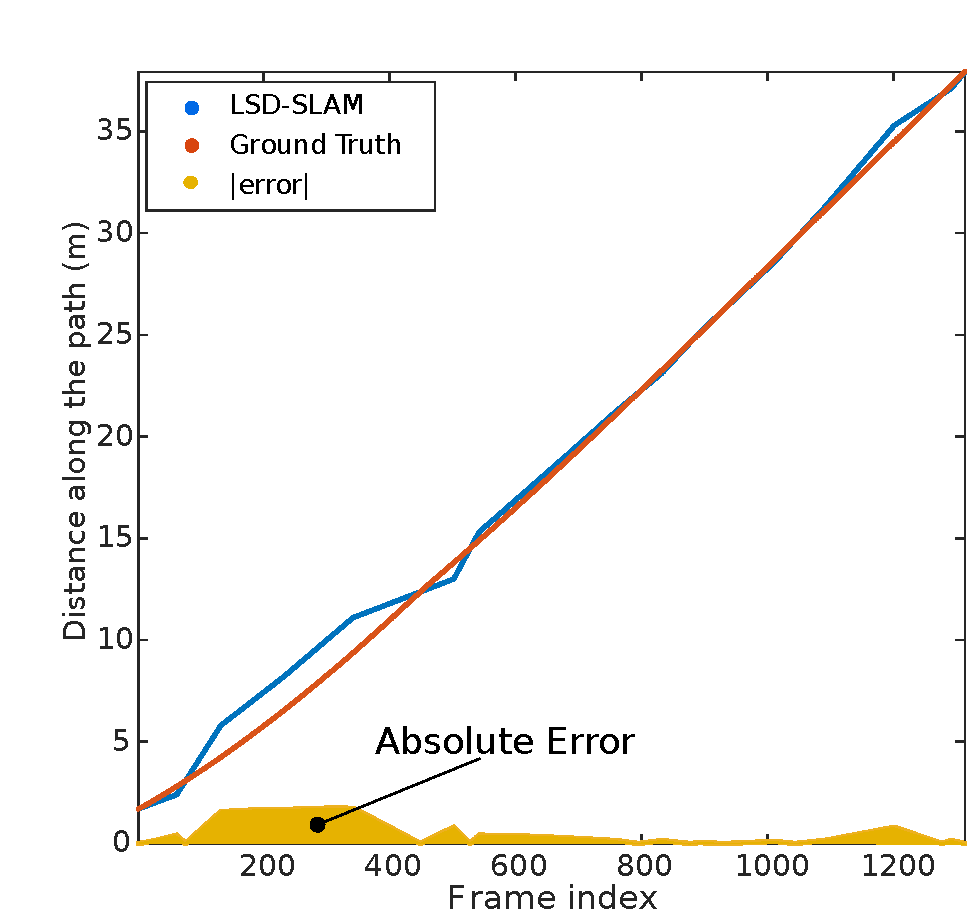
\includegraphics[width=0.45\textwidth]	{./gfx/Chapter04/lsd_slam_good.pdf}\label{fig:slamperfA}
	}
	\quad
	\subfloat[(b)][Errors obtained from another experiment using LSD-SLAM. In this case, the absolute error peaked at around $5$ m. ]{
	\setlength\figureheight{0.5\textwidth}
	\setlength\figurewidth{0.8\textwidth}
	% This file was created by matlab2tikz.
% Minimal pgfplots version: 1.3
%
%The latest updates can be retrieved from
%  http://www.mathworks.com/matlabcentral/fileexchange/22022-matlab2tikz
%where you can also make suggestions and rate matlab2tikz.
%
\definecolor{mycolor1}{rgb}{0.00000,0.44700,0.74100}%
\definecolor{mycolor2}{rgb}{0.85000,0.32500,0.09800}%
\definecolor{mycolor3}{rgb}{0.92900,0.69400,0.12500}%
%
\begin{tikzpicture}

\begin{axis}[%
width=0.95092\figurewidth,
height=\figureheight,
at={(0\figurewidth,0\figureheight)},
scale only axis,
xmin=1,
xmax=1500,
xlabel={Frame index},
ymin=0,
ymax=4380,
yticklabels={0,5,10,15,20,25,30,35},
ylabel={Distance along the path (m)},
legend style={at={(0.03,0.97)},anchor=north west,legend cell align=left,align=left,draw=white!15!black}
]
\addplot [color=mycolor1,mark size=1.3pt,only marks,mark=*,mark options={solid}]
  table[row sep=crcr]{%
1	212.86\\
2	214.29\\
3	215.71\\
4	217.14\\
5	218.57\\
6	220\\
7	221.43\\
8	222.86\\
9	224.29\\
10	225.71\\
11	227.14\\
12	228.57\\
13	230\\
14	231.43\\
15	232.86\\
16	234.29\\
17	235.71\\
18	237.14\\
19	238.57\\
20	240\\
21	243.27\\
22	246.54\\
23	249.81\\
24	253.08\\
25	256.35\\
26	259.62\\
27	262.88\\
28	266.15\\
29	269.42\\
30	272.69\\
31	275.96\\
32	279.23\\
33	282.5\\
34	285.77\\
35	289.04\\
36	292.31\\
37	295.58\\
38	298.85\\
39	302.12\\
40	305.38\\
41	308.65\\
42	311.92\\
43	315.19\\
44	318.46\\
45	321.73\\
46	325\\
47	328.27\\
48	331.54\\
49	334.81\\
50	338.08\\
51	341.35\\
52	344.62\\
53	347.88\\
54	351.15\\
55	354.42\\
56	357.69\\
57	360.96\\
58	364.23\\
59	367.5\\
60	370.77\\
61	374.04\\
62	377.31\\
63	380.58\\
64	383.85\\
65	387.12\\
66	390.38\\
67	393.65\\
68	396.92\\
69	400.19\\
70	403.46\\
71	406.73\\
72	410\\
73	413.27\\
74	416.54\\
75	419.81\\
76	423.08\\
77	426.35\\
78	429.62\\
79	432.88\\
80	436.15\\
81	439.42\\
82	442.69\\
83	445.96\\
84	449.23\\
85	452.5\\
86	455.77\\
87	459.04\\
88	462.31\\
89	465.58\\
90	468.85\\
91	472.12\\
92	475.38\\
93	478.65\\
94	481.92\\
95	485.19\\
96	488.46\\
97	491.73\\
98	495\\
99	498.27\\
100	501.54\\
101	504.81\\
102	508.08\\
103	511.35\\
104	514.62\\
105	517.88\\
106	521.15\\
107	524.42\\
108	527.69\\
109	530.96\\
110	534.23\\
111	537.5\\
112	540.77\\
113	544.04\\
114	547.31\\
115	550.58\\
116	553.85\\
117	557.12\\
118	560.38\\
119	563.65\\
120	566.92\\
121	570.19\\
122	573.46\\
123	576.73\\
124	580\\
125	585\\
126	590\\
127	595\\
128	600\\
129	605\\
130	610\\
131	615\\
132	620\\
133	625\\
134	630\\
135	635\\
136	640\\
137	645\\
138	650\\
139	655\\
140	660\\
141	665\\
142	670\\
143	675\\
144	680\\
145	685\\
146	690\\
147	695\\
148	700\\
149	705\\
150	710\\
151	715\\
152	720\\
153	725\\
154	730\\
155	735\\
156	740\\
157	745\\
158	750\\
159	755\\
160	760\\
161	765\\
162	770\\
163	775\\
164	780\\
165	785\\
166	790\\
167	795\\
168	800\\
169	805\\
170	810\\
171	815\\
172	820\\
173	821.81\\
174	823.62\\
175	825.44\\
176	827.25\\
177	829.06\\
178	830.88\\
179	832.69\\
180	834.5\\
181	836.31\\
182	838.12\\
183	839.94\\
184	841.75\\
185	843.56\\
186	845.38\\
187	847.19\\
188	849\\
189	850.81\\
190	852.62\\
191	854.44\\
192	856.25\\
193	858.06\\
194	859.88\\
195	861.69\\
196	863.5\\
197	865.31\\
198	867.12\\
199	868.94\\
200	870.75\\
201	872.56\\
202	874.38\\
203	876.19\\
204	878\\
205	879.81\\
206	881.62\\
207	883.44\\
208	885.25\\
209	887.06\\
210	888.88\\
211	890.69\\
212	892.5\\
213	894.31\\
214	896.12\\
215	897.94\\
216	899.75\\
217	901.56\\
218	903.38\\
219	905.19\\
220	907\\
221	908.81\\
222	910.62\\
223	912.44\\
224	914.25\\
225	916.06\\
226	917.88\\
227	919.69\\
228	921.5\\
229	923.31\\
230	925.12\\
231	926.94\\
232	928.75\\
233	930.56\\
234	932.38\\
235	934.19\\
236	936\\
237	937.81\\
238	939.62\\
239	941.44\\
240	943.25\\
241	945.06\\
242	946.88\\
243	948.69\\
244	950.5\\
245	952.31\\
246	954.12\\
247	955.94\\
248	957.75\\
249	959.56\\
250	961.38\\
251	963.19\\
252	965\\
253	966.81\\
254	968.62\\
255	970.44\\
256	972.25\\
257	974.06\\
258	975.88\\
259	977.69\\
260	979.5\\
261	981.31\\
262	983.12\\
263	984.94\\
264	986.75\\
265	988.56\\
266	990.38\\
267	992.19\\
268	994\\
269	995.81\\
270	997.62\\
271	999.44\\
272	1001.25\\
273	1003.06\\
274	1004.88\\
275	1006.69\\
276	1008.5\\
277	1010.31\\
278	1012.12\\
279	1013.94\\
280	1015.75\\
281	1017.56\\
282	1019.38\\
283	1021.19\\
284	1023\\
285	1024.81\\
286	1026.62\\
287	1028.44\\
288	1030.25\\
289	1032.06\\
290	1033.88\\
291	1035.69\\
292	1037.5\\
293	1039.31\\
294	1041.12\\
295	1042.94\\
296	1044.75\\
297	1046.56\\
298	1048.38\\
299	1050.19\\
300	1052\\
301	1053.81\\
302	1055.62\\
303	1057.44\\
304	1059.25\\
305	1061.06\\
306	1062.88\\
307	1064.69\\
308	1066.5\\
309	1068.31\\
310	1070.12\\
311	1071.94\\
312	1073.75\\
313	1075.56\\
314	1077.38\\
315	1079.19\\
316	1081\\
317	1082.81\\
318	1084.62\\
319	1086.44\\
320	1088.25\\
321	1090.06\\
322	1091.88\\
323	1093.69\\
324	1095.5\\
325	1097.31\\
326	1099.12\\
327	1100.94\\
328	1102.75\\
329	1104.56\\
330	1106.38\\
331	1108.19\\
332	1110\\
333	1110.68\\
334	1111.36\\
335	1112.04\\
336	1112.71\\
337	1113.39\\
338	1114.07\\
339	1114.75\\
340	1115.43\\
341	1116.11\\
342	1116.79\\
343	1117.46\\
344	1118.14\\
345	1118.82\\
346	1119.5\\
347	1120.18\\
348	1120.86\\
349	1121.54\\
350	1122.21\\
351	1122.89\\
352	1123.57\\
353	1124.25\\
354	1124.93\\
355	1125.61\\
356	1126.29\\
357	1126.96\\
358	1127.64\\
359	1128.32\\
360	1129\\
361	1129.68\\
362	1130.36\\
363	1131.04\\
364	1131.71\\
365	1132.39\\
366	1133.07\\
367	1133.75\\
368	1134.43\\
369	1135.11\\
370	1135.79\\
371	1136.46\\
372	1137.14\\
373	1137.82\\
374	1138.5\\
375	1139.18\\
376	1139.86\\
377	1140.54\\
378	1141.21\\
379	1141.89\\
380	1142.57\\
381	1143.25\\
382	1143.93\\
383	1144.61\\
384	1145.29\\
385	1145.96\\
386	1146.64\\
387	1147.32\\
388	1148\\
389	1148.68\\
390	1149.36\\
391	1150.04\\
392	1150.71\\
393	1151.39\\
394	1152.07\\
395	1152.75\\
396	1153.43\\
397	1154.11\\
398	1154.79\\
399	1155.46\\
400	1156.14\\
401	1156.82\\
402	1157.5\\
403	1158.18\\
404	1158.86\\
405	1159.54\\
406	1160.21\\
407	1160.89\\
408	1161.57\\
409	1162.25\\
410	1162.93\\
411	1163.61\\
412	1164.29\\
413	1164.96\\
414	1165.64\\
415	1166.32\\
416	1167\\
417	1167.68\\
418	1168.36\\
419	1169.04\\
420	1169.71\\
421	1170.39\\
422	1171.07\\
423	1171.75\\
424	1172.43\\
425	1173.11\\
426	1173.79\\
427	1174.46\\
428	1175.14\\
429	1175.82\\
430	1176.5\\
431	1177.18\\
432	1177.86\\
433	1178.54\\
434	1179.21\\
435	1179.89\\
436	1180.57\\
437	1181.25\\
438	1181.93\\
439	1182.61\\
440	1183.29\\
441	1183.96\\
442	1184.64\\
443	1185.32\\
444	1186\\
445	1186.68\\
446	1187.36\\
447	1188.04\\
448	1188.71\\
449	1189.39\\
450	1190.07\\
451	1190.75\\
452	1191.43\\
453	1192.11\\
454	1192.79\\
455	1193.46\\
456	1194.14\\
457	1194.82\\
458	1195.5\\
459	1196.18\\
460	1196.86\\
461	1197.54\\
462	1198.21\\
463	1198.89\\
464	1199.57\\
465	1200.25\\
466	1200.93\\
467	1201.61\\
468	1202.29\\
469	1202.96\\
470	1203.64\\
471	1204.32\\
472	1205\\
473	1205.68\\
474	1206.36\\
475	1207.04\\
476	1207.71\\
477	1208.39\\
478	1209.07\\
479	1209.75\\
480	1210.43\\
481	1211.11\\
482	1211.79\\
483	1212.46\\
484	1213.14\\
485	1213.82\\
486	1214.5\\
487	1215.18\\
488	1215.86\\
489	1216.54\\
490	1217.21\\
491	1217.89\\
492	1218.57\\
493	1219.25\\
494	1219.93\\
495	1220.61\\
496	1221.29\\
497	1221.96\\
498	1222.64\\
499	1223.32\\
500	1224\\
501	1224.68\\
502	1225.36\\
503	1226.04\\
504	1226.71\\
505	1227.39\\
506	1228.07\\
507	1228.75\\
508	1229.43\\
509	1230.11\\
510	1230.79\\
511	1231.46\\
512	1232.14\\
513	1232.82\\
514	1233.5\\
515	1234.18\\
516	1234.86\\
517	1235.54\\
518	1236.21\\
519	1236.89\\
520	1237.57\\
521	1238.25\\
522	1238.93\\
523	1239.61\\
524	1240.29\\
525	1240.96\\
526	1241.64\\
527	1242.32\\
528	1243\\
529	1243.68\\
530	1244.36\\
531	1245.04\\
532	1245.71\\
533	1246.39\\
534	1247.07\\
535	1247.75\\
536	1248.43\\
537	1249.11\\
538	1249.79\\
539	1250.46\\
540	1251.14\\
541	1251.82\\
542	1252.5\\
543	1253.18\\
544	1253.86\\
545	1254.54\\
546	1255.21\\
547	1255.89\\
548	1256.57\\
549	1257.25\\
550	1257.93\\
551	1258.61\\
552	1259.29\\
553	1259.96\\
554	1260.64\\
555	1261.32\\
556	1262\\
557	1262.68\\
558	1263.36\\
559	1264.04\\
560	1264.71\\
561	1265.39\\
562	1266.07\\
563	1266.75\\
564	1267.43\\
565	1268.11\\
566	1268.79\\
567	1269.46\\
568	1270.14\\
569	1270.82\\
570	1271.5\\
571	1272.18\\
572	1272.86\\
573	1273.54\\
574	1274.21\\
575	1274.89\\
576	1275.57\\
577	1276.25\\
578	1276.93\\
579	1277.61\\
580	1278.29\\
581	1278.96\\
582	1279.64\\
583	1280.32\\
584	1281\\
585	1281.68\\
586	1282.36\\
587	1283.04\\
588	1283.71\\
589	1284.39\\
590	1285.07\\
591	1285.75\\
592	1286.43\\
593	1287.11\\
594	1287.79\\
595	1288.46\\
596	1289.14\\
597	1289.82\\
598	1290.5\\
599	1291.18\\
600	1291.86\\
601	1292.54\\
602	1293.21\\
603	1293.89\\
604	1294.57\\
605	1295.25\\
606	1295.93\\
607	1296.61\\
608	1297.29\\
609	1297.96\\
610	1298.64\\
611	1299.32\\
612	1300\\
613	1303.59\\
614	1307.19\\
615	1310.78\\
616	1314.38\\
617	1317.97\\
618	1321.56\\
619	1325.16\\
620	1328.75\\
621	1332.34\\
622	1335.94\\
623	1339.53\\
624	1343.12\\
625	1346.72\\
626	1350.31\\
627	1353.91\\
628	1357.5\\
629	1361.09\\
630	1364.69\\
631	1368.28\\
632	1371.88\\
633	1375.47\\
634	1379.06\\
635	1382.66\\
636	1386.25\\
637	1389.84\\
638	1393.44\\
639	1397.03\\
640	1400.62\\
641	1404.22\\
642	1407.81\\
643	1411.41\\
644	1415\\
645	1418.59\\
646	1422.19\\
647	1425.78\\
648	1429.38\\
649	1432.97\\
650	1436.56\\
651	1440.16\\
652	1443.75\\
653	1447.34\\
654	1450.94\\
655	1454.53\\
656	1458.12\\
657	1461.72\\
658	1465.31\\
659	1468.91\\
660	1472.5\\
661	1476.09\\
662	1479.69\\
663	1483.28\\
664	1486.88\\
665	1490.47\\
666	1494.06\\
667	1497.66\\
668	1501.25\\
669	1504.84\\
670	1508.44\\
671	1512.03\\
672	1515.62\\
673	1519.22\\
674	1522.81\\
675	1526.41\\
676	1530\\
677	1533.65\\
678	1537.31\\
679	1540.96\\
680	1544.62\\
681	1548.27\\
682	1551.92\\
683	1555.58\\
684	1559.23\\
685	1562.88\\
686	1566.54\\
687	1570.19\\
688	1573.85\\
689	1577.5\\
690	1581.15\\
691	1584.81\\
692	1588.46\\
693	1592.12\\
694	1595.77\\
695	1599.42\\
696	1603.08\\
697	1606.73\\
698	1610.38\\
699	1614.04\\
700	1617.69\\
701	1621.35\\
702	1625\\
703	1628.65\\
704	1632.31\\
705	1635.96\\
706	1639.62\\
707	1643.27\\
708	1646.92\\
709	1650.58\\
710	1654.23\\
711	1657.88\\
712	1661.54\\
713	1665.19\\
714	1668.85\\
715	1672.5\\
716	1676.15\\
717	1679.81\\
718	1683.46\\
719	1687.12\\
720	1690.77\\
721	1694.42\\
722	1698.08\\
723	1701.73\\
724	1705.38\\
725	1709.04\\
726	1712.69\\
727	1716.35\\
728	1720\\
729	1723.65\\
730	1727.31\\
731	1730.96\\
732	1734.62\\
733	1738.27\\
734	1741.92\\
735	1745.58\\
736	1749.23\\
737	1752.88\\
738	1756.54\\
739	1760.19\\
740	1763.85\\
741	1767.5\\
742	1771.15\\
743	1774.81\\
744	1778.46\\
745	1782.12\\
746	1785.77\\
747	1789.42\\
748	1793.08\\
749	1796.73\\
750	1800.38\\
751	1804.04\\
752	1807.69\\
753	1811.35\\
754	1815\\
755	1818.65\\
756	1822.31\\
757	1825.96\\
758	1829.62\\
759	1833.27\\
760	1836.92\\
761	1840.58\\
762	1844.23\\
763	1847.88\\
764	1851.54\\
765	1855.19\\
766	1858.85\\
767	1862.5\\
768	1866.15\\
769	1869.81\\
770	1873.46\\
771	1877.12\\
772	1880.77\\
773	1884.42\\
774	1888.08\\
775	1891.73\\
776	1895.38\\
777	1899.04\\
778	1902.69\\
779	1906.35\\
780	1910\\
781	1912.5\\
782	1915\\
783	1917.5\\
784	1920\\
785	1922.5\\
786	1925\\
787	1927.5\\
788	1930\\
789	1932.5\\
790	1935\\
791	1937.5\\
792	1940\\
793	1942.5\\
794	1945\\
795	1947.5\\
796	1950\\
797	1952.5\\
798	1955\\
799	1957.5\\
800	1960\\
801	1962.5\\
802	1965\\
803	1967.5\\
804	1970\\
805	1972.5\\
806	1975\\
807	1977.5\\
808	1980\\
809	1982.5\\
810	1985\\
811	1987.5\\
812	1990\\
813	1992.5\\
814	1995\\
815	1997.5\\
816	2000\\
817	2002.5\\
818	2005\\
819	2007.5\\
820	2010\\
821	2012.5\\
822	2015\\
823	2017.5\\
824	2020\\
825	2022.5\\
826	2025\\
827	2027.5\\
828	2030\\
829	2032.5\\
830	2035\\
831	2037.5\\
832	2040\\
833	2042.5\\
834	2045\\
835	2047.5\\
836	2050\\
837	2052.5\\
838	2055\\
839	2057.5\\
840	2060\\
841	2062.5\\
842	2065\\
843	2067.5\\
844	2070\\
845	2072.5\\
846	2075\\
847	2077.5\\
848	2080\\
849	2082.5\\
850	2085\\
851	2087.5\\
852	2090\\
853	2092.5\\
854	2095\\
855	2097.5\\
856	2100\\
857	2102.5\\
858	2105\\
859	2107.5\\
860	2110\\
861	2112.5\\
862	2115\\
863	2117.5\\
864	2120\\
865	2122.5\\
866	2125\\
867	2127.5\\
868	2130\\
869	2134.5\\
870	2139\\
871	2143.5\\
872	2148\\
873	2152.5\\
874	2157\\
875	2161.5\\
876	2166\\
877	2170.5\\
878	2175\\
879	2179.5\\
880	2184\\
881	2188.5\\
882	2193\\
883	2197.5\\
884	2202\\
885	2206.5\\
886	2211\\
887	2215.5\\
888	2220\\
889	2224.5\\
890	2229\\
891	2233.5\\
892	2238\\
893	2242.5\\
894	2247\\
895	2251.5\\
896	2256\\
897	2260.5\\
898	2265\\
899	2269.5\\
900	2274\\
901	2278.5\\
902	2283\\
903	2287.5\\
904	2292\\
905	2296.5\\
906	2301\\
907	2305.5\\
908	2310\\
909	2313.12\\
910	2316.25\\
911	2319.38\\
912	2322.5\\
913	2325.62\\
914	2328.75\\
915	2331.88\\
916	2335\\
917	2338.12\\
918	2341.25\\
919	2344.38\\
920	2347.5\\
921	2350.62\\
922	2353.75\\
923	2356.88\\
924	2360\\
925	2363.12\\
926	2366.25\\
927	2369.38\\
928	2372.5\\
929	2375.62\\
930	2378.75\\
931	2381.88\\
932	2385\\
933	2388.12\\
934	2391.25\\
935	2394.38\\
936	2397.5\\
937	2400.62\\
938	2403.75\\
939	2406.88\\
940	2410\\
941	2413.12\\
942	2416.25\\
943	2419.38\\
944	2422.5\\
945	2425.62\\
946	2428.75\\
947	2431.88\\
948	2435\\
949	2438.12\\
950	2441.25\\
951	2444.38\\
952	2447.5\\
953	2450.62\\
954	2453.75\\
955	2456.88\\
956	2460\\
957	2463.12\\
958	2466.25\\
959	2469.38\\
960	2472.5\\
961	2475.62\\
962	2478.75\\
963	2481.88\\
964	2485\\
965	2488.12\\
966	2491.25\\
967	2494.38\\
968	2497.5\\
969	2500.62\\
970	2503.75\\
971	2506.88\\
972	2510\\
973	2513.98\\
974	2517.95\\
975	2521.93\\
976	2525.91\\
977	2529.89\\
978	2533.86\\
979	2537.84\\
980	2541.82\\
981	2545.8\\
982	2549.77\\
983	2553.75\\
984	2557.73\\
985	2561.7\\
986	2565.68\\
987	2569.66\\
988	2573.64\\
989	2577.61\\
990	2581.59\\
991	2585.57\\
992	2589.55\\
993	2593.52\\
994	2597.5\\
995	2601.48\\
996	2605.45\\
997	2609.43\\
998	2613.41\\
999	2617.39\\
1000	2621.36\\
1001	2625.34\\
1002	2629.32\\
1003	2633.3\\
1004	2637.27\\
1005	2641.25\\
1006	2645.23\\
1007	2649.2\\
1008	2653.18\\
1009	2657.16\\
1010	2661.14\\
1011	2665.11\\
1012	2669.09\\
1013	2673.07\\
1014	2677.05\\
1015	2681.02\\
1016	2685\\
1017	2688.98\\
1018	2692.95\\
1019	2696.93\\
1020	2700.91\\
1021	2704.89\\
1022	2708.86\\
1023	2712.84\\
1024	2716.82\\
1025	2720.8\\
1026	2724.77\\
1027	2728.75\\
1028	2732.73\\
1029	2736.7\\
1030	2740.68\\
1031	2744.66\\
1032	2748.64\\
1033	2752.61\\
1034	2756.59\\
1035	2760.57\\
1036	2764.55\\
1037	2768.52\\
1038	2772.5\\
1039	2776.48\\
1040	2780.45\\
1041	2784.43\\
1042	2788.41\\
1043	2792.39\\
1044	2796.36\\
1045	2800.34\\
1046	2804.32\\
1047	2808.3\\
1048	2812.27\\
1049	2816.25\\
1050	2820.23\\
1051	2824.2\\
1052	2828.18\\
1053	2832.16\\
1054	2836.14\\
1055	2840.11\\
1056	2844.09\\
1057	2848.07\\
1058	2852.05\\
1059	2856.02\\
1060	2860\\
1061	2864.22\\
1062	2868.44\\
1063	2872.66\\
1064	2876.88\\
1065	2881.09\\
1066	2885.31\\
1067	2889.53\\
1068	2893.75\\
1069	2897.97\\
1070	2902.19\\
1071	2906.41\\
1072	2910.62\\
1073	2914.84\\
1074	2919.06\\
1075	2923.28\\
1076	2927.5\\
1077	2931.72\\
1078	2935.94\\
1079	2940.16\\
1080	2944.38\\
1081	2948.59\\
1082	2952.81\\
1083	2957.03\\
1084	2961.25\\
1085	2965.47\\
1086	2969.69\\
1087	2973.91\\
1088	2978.12\\
1089	2982.34\\
1090	2986.56\\
1091	2990.78\\
1092	2995\\
1093	2999.22\\
1094	3003.44\\
1095	3007.66\\
1096	3011.88\\
1097	3016.09\\
1098	3020.31\\
1099	3024.53\\
1100	3028.75\\
1101	3032.97\\
1102	3037.19\\
1103	3041.41\\
1104	3045.62\\
1105	3049.84\\
1106	3054.06\\
1107	3058.28\\
1108	3062.5\\
1109	3066.72\\
1110	3070.94\\
1111	3075.16\\
1112	3079.38\\
1113	3083.59\\
1114	3087.81\\
1115	3092.03\\
1116	3096.25\\
1117	3100.47\\
1118	3104.69\\
1119	3108.91\\
1120	3113.12\\
1121	3117.34\\
1122	3121.56\\
1123	3125.78\\
1124	3130\\
1125	3133.12\\
1126	3136.25\\
1127	3139.38\\
1128	3142.5\\
1129	3145.62\\
1130	3148.75\\
1131	3151.88\\
1132	3155\\
1133	3158.12\\
1134	3161.25\\
1135	3164.38\\
1136	3167.5\\
1137	3170.62\\
1138	3173.75\\
1139	3176.88\\
1140	3180\\
1141	3183.12\\
1142	3186.25\\
1143	3189.38\\
1144	3192.5\\
1145	3195.62\\
1146	3198.75\\
1147	3201.88\\
1148	3205\\
1149	3208.12\\
1150	3211.25\\
1151	3214.38\\
1152	3217.5\\
1153	3220.62\\
1154	3223.75\\
1155	3226.88\\
1156	3230\\
1157	3233.12\\
1158	3236.25\\
1159	3239.38\\
1160	3242.5\\
1161	3245.62\\
1162	3248.75\\
1163	3251.88\\
1164	3255\\
1165	3258.12\\
1166	3261.25\\
1167	3264.38\\
1168	3267.5\\
1169	3270.62\\
1170	3273.75\\
1171	3276.88\\
1172	3280\\
1173	3283.12\\
1174	3286.25\\
1175	3289.38\\
1176	3292.5\\
1177	3295.62\\
1178	3298.75\\
1179	3301.88\\
1180	3305\\
1181	3308.12\\
1182	3311.25\\
1183	3314.38\\
1184	3317.5\\
1185	3320.62\\
1186	3323.75\\
1187	3326.88\\
1188	3330\\
1189	3333.12\\
1190	3336.25\\
1191	3339.38\\
1192	3342.5\\
1193	3345.62\\
1194	3348.75\\
1195	3351.88\\
1196	3355\\
1197	3358.12\\
1198	3361.25\\
1199	3364.38\\
1200	3367.5\\
1201	3370.62\\
1202	3373.75\\
1203	3376.88\\
1204	3380\\
1205	3383.12\\
1206	3386.25\\
1207	3389.38\\
1208	3392.5\\
1209	3395.62\\
1210	3398.75\\
1211	3401.88\\
1212	3405\\
1213	3408.12\\
1214	3411.25\\
1215	3414.38\\
1216	3417.5\\
1217	3420.62\\
1218	3423.75\\
1219	3426.88\\
1220	3430\\
1221	3433.12\\
1222	3436.25\\
1223	3439.38\\
1224	3442.5\\
1225	3445.62\\
1226	3448.75\\
1227	3451.88\\
1228	3455\\
1229	3458.12\\
1230	3461.25\\
1231	3464.38\\
1232	3467.5\\
1233	3470.62\\
1234	3473.75\\
1235	3476.88\\
1236	3480\\
1237	3483.12\\
1238	3486.25\\
1239	3489.38\\
1240	3492.5\\
1241	3495.62\\
1242	3498.75\\
1243	3501.88\\
1244	3505\\
1245	3508.12\\
1246	3511.25\\
1247	3514.38\\
1248	3517.5\\
1249	3520.62\\
1250	3523.75\\
1251	3526.88\\
1252	3530\\
1253	3533.75\\
1254	3537.5\\
1255	3541.25\\
1256	3545\\
1257	3548.75\\
1258	3552.5\\
1259	3556.25\\
1260	3560\\
1261	3563.75\\
1262	3567.5\\
1263	3571.25\\
1264	3575\\
1265	3578.75\\
1266	3582.5\\
1267	3586.25\\
1268	3590\\
1269	3593.75\\
1270	3597.5\\
1271	3601.25\\
1272	3605\\
1273	3608.75\\
1274	3612.5\\
1275	3616.25\\
1276	3620\\
1277	3623.75\\
1278	3627.5\\
1279	3631.25\\
1280	3635\\
1281	3638.75\\
1282	3642.5\\
1283	3646.25\\
1284	3650\\
1285	3653.75\\
1286	3657.5\\
1287	3661.25\\
1288	3665\\
1289	3668.75\\
1290	3672.5\\
1291	3676.25\\
1292	3680\\
1293	3683.75\\
1294	3687.5\\
1295	3691.25\\
1296	3695\\
1297	3698.75\\
1298	3702.5\\
1299	3706.25\\
1300	3710\\
1301	3713.75\\
1302	3717.5\\
1303	3721.25\\
1304	3725\\
1305	3728.75\\
1306	3732.5\\
1307	3736.25\\
1308	3740\\
1309	3743.75\\
1310	3747.5\\
1311	3751.25\\
1312	3755\\
1313	3758.75\\
1314	3762.5\\
1315	3766.25\\
1316	3770\\
1317	3773.75\\
1318	3777.5\\
1319	3781.25\\
1320	3785\\
1321	3788.75\\
1322	3792.5\\
1323	3796.25\\
1324	3800\\
1325	3803.75\\
1326	3807.5\\
1327	3811.25\\
1328	3815\\
1329	3818.75\\
1330	3822.5\\
1331	3826.25\\
1332	3830\\
1333	3833.75\\
1334	3837.5\\
1335	3841.25\\
1336	3845\\
1337	3848.75\\
1338	3852.5\\
1339	3856.25\\
1340	3860\\
1341	3862.08\\
1342	3864.17\\
1343	3866.25\\
1344	3868.33\\
1345	3870.42\\
1346	3872.5\\
1347	3874.58\\
1348	3876.67\\
1349	3878.75\\
1350	3880.83\\
1351	3882.92\\
1352	3885\\
1353	3887.08\\
1354	3889.17\\
1355	3891.25\\
1356	3893.33\\
1357	3895.42\\
1358	3897.5\\
1359	3899.58\\
1360	3901.67\\
1361	3903.75\\
1362	3905.83\\
1363	3907.92\\
1364	3910\\
1365	3912.08\\
1366	3914.17\\
1367	3916.25\\
1368	3918.33\\
1369	3920.42\\
1370	3922.5\\
1371	3924.58\\
1372	3926.67\\
1373	3928.75\\
1374	3930.83\\
1375	3932.92\\
1376	3935\\
1377	3937.08\\
1378	3939.17\\
1379	3941.25\\
1380	3943.33\\
1381	3945.42\\
1382	3947.5\\
1383	3949.58\\
1384	3951.67\\
1385	3953.75\\
1386	3955.83\\
1387	3957.92\\
1388	3960\\
1389	3962.08\\
1390	3964.17\\
1391	3966.25\\
1392	3968.33\\
1393	3970.42\\
1394	3972.5\\
1395	3974.58\\
1396	3976.67\\
1397	3978.75\\
1398	3980.83\\
1399	3982.92\\
1400	3985\\
1401	3987.08\\
1402	3989.17\\
1403	3991.25\\
1404	3993.33\\
1405	3995.42\\
1406	3997.5\\
1407	3999.58\\
1408	4001.67\\
1409	4003.75\\
1410	4005.83\\
1411	4007.92\\
1412	4010\\
1413	4012.08\\
1414	4014.17\\
1415	4016.25\\
1416	4018.33\\
1417	4020.42\\
1418	4022.5\\
1419	4024.58\\
1420	4026.67\\
1421	4028.75\\
1422	4030.83\\
1423	4032.92\\
1424	4035\\
1425	4037.08\\
1426	4039.17\\
1427	4041.25\\
1428	4043.33\\
1429	4045.42\\
1430	4047.5\\
1431	4049.58\\
1432	4051.67\\
1433	4053.75\\
1434	4055.83\\
1435	4057.92\\
1436	4060\\
1437	4065.42\\
1438	4070.83\\
1439	4076.25\\
1440	4081.67\\
1441	4087.08\\
1442	4092.5\\
1443	4097.92\\
1444	4103.33\\
1445	4108.75\\
1446	4114.17\\
1447	4119.58\\
1448	4125\\
1449	4130.42\\
1450	4135.83\\
1451	4141.25\\
1452	4146.67\\
1453	4152.08\\
1454	4157.5\\
1455	4162.92\\
1456	4168.33\\
1457	4173.75\\
1458	4179.17\\
1459	4184.58\\
1460	4190\\
1461	4195.42\\
1462	4200.83\\
1463	4206.25\\
1464	4211.67\\
1465	4217.08\\
1466	4222.5\\
1467	4227.92\\
1468	4233.33\\
1469	4238.75\\
1470	4244.17\\
1471	4249.58\\
1472	4255\\
1473	4260.42\\
1474	4265.83\\
1475	4271.25\\
1476	4276.67\\
1477	4282.08\\
1478	4287.5\\
1479	4292.92\\
1480	4298.33\\
1481	4303.75\\
1482	4309.17\\
1483	4314.58\\
1484	4320\\
1485	4323.75\\
1486	4327.5\\
1487	4331.25\\
1488	4335\\
1489	4338.75\\
1490	4342.5\\
1491	4346.25\\
1492	4350\\
1493	4353.75\\
1494	4357.5\\
1495	4361.25\\
1496	4365\\
1497	4368.75\\
1498	4372.5\\
1499	4376.25\\
1500	4380\\
};
\addlegendentry{LSD-SLAM};

\addplot [color=mycolor2,mark size=1.3pt,only marks,mark=*,mark options={solid}]
  table[row sep=crcr]{%
1	212.86\\
2	214.641734651949\\
3	216.437260907038\\
4	218.238875275567\\
5	220.026907993932\\
6	221.823458121644\\
7	223.626767938565\\
8	225.441127955297\\
9	227.256460831336\\
10	229.078372356498\\
11	230.911575808738\\
12	232.753340412754\\
13	234.608108607758\\
14	236.465333712739\\
15	238.333162409078\\
16	240.205687089554\\
17	242.097780405477\\
18	243.991434929776\\
19	245.892956287896\\
20	247.805998272663\\
21	249.721608266439\\
22	251.64132462003\\
23	253.564825106337\\
24	255.495499516794\\
25	257.425489922186\\
26	259.358641149587\\
27	261.29782155451\\
28	263.243740827787\\
29	265.192794993365\\
30	267.14004580437\\
31	269.103508459304\\
32	271.073636431431\\
33	273.046430150075\\
34	275.026989483158\\
35	277.014311321873\\
36	279.006372421747\\
37	281.003690232238\\
38	283.010418767346\\
39	285.026663677862\\
40	287.043871682151\\
41	289.067150455827\\
42	291.099491148141\\
43	293.137407487467\\
44	295.176418174043\\
45	297.221098879855\\
46	299.270765526933\\
47	301.323923531052\\
48	303.378856791588\\
49	305.438738171695\\
50	307.50176896999\\
51	309.568380019182\\
52	311.638856230731\\
53	313.71233405498\\
54	315.79487079396\\
55	317.882584885311\\
56	319.975016498722\\
57	322.072730629434\\
58	324.174849144796\\
59	326.280475781768\\
60	328.390922915189\\
61	330.507271162375\\
62	332.62701081164\\
63	334.748694247652\\
64	336.868281344702\\
65	338.992451600638\\
66	341.126864480122\\
67	343.266191841986\\
68	345.410908297658\\
69	347.560343920234\\
70	349.713802269703\\
71	351.869818015999\\
72	354.028508765498\\
73	356.18922826659\\
74	358.351362629937\\
75	360.515420782568\\
76	362.682791142739\\
77	364.851812583454\\
78	367.026576546837\\
79	369.205200457057\\
80	371.388646577223\\
81	373.576000374462\\
82	375.768566604938\\
83	377.966051424249\\
84	380.167421653487\\
85	382.3715093096\\
86	384.577974930679\\
87	386.792491165513\\
88	389.012864253133\\
89	391.245989787508\\
90	393.477334030398\\
91	395.706772943375\\
92	397.942554685617\\
93	400.186402702405\\
94	402.43416378035\\
95	404.684639227452\\
96	406.936931854279\\
97	409.188904808571\\
98	411.446781329862\\
99	413.70442892701\\
100	415.964844698904\\
101	418.227511645188\\
102	420.49313384311\\
103	422.761522167772\\
104	425.032178175059\\
105	427.304725018011\\
106	429.584288228921\\
107	431.86776914898\\
108	434.150953754576\\
109	436.437718476662\\
110	438.728453953511\\
111	441.026478279355\\
112	443.33376170529\\
113	445.643412584797\\
114	447.956054713975\\
115	450.270820012994\\
116	452.590087479053\\
117	454.912090549258\\
118	457.23614875402\\
119	459.563952480143\\
120	461.892967709466\\
121	464.222114953304\\
122	466.552056957702\\
123	468.885211306354\\
124	471.2247993313\\
125	473.566372940329\\
126	475.911720251258\\
127	478.259930924711\\
128	480.609457797004\\
129	482.961068567395\\
130	485.314396220926\\
131	487.669838526097\\
132	490.02768517721\\
133	492.387674834586\\
134	494.749610114119\\
135	497.115430380805\\
136	499.487537333006\\
137	501.863385870578\\
138	504.240690566532\\
139	506.620842685928\\
140	509.001164244643\\
141	511.382972423152\\
142	513.766446331236\\
143	516.153114843274\\
144	518.541781561306\\
145	520.932610336828\\
146	523.325077296282\\
147	525.720202322105\\
148	528.117709852666\\
149	530.516863218947\\
150	532.916481117409\\
151	535.317740432021\\
152	537.720638366885\\
153	540.126115595016\\
154	542.534246676158\\
155	544.944849832441\\
156	547.358955840265\\
157	549.776084020508\\
158	552.195964425166\\
159	554.619743368833\\
160	557.046893501025\\
161	559.4766522349\\
162	561.91002584476\\
163	564.345865138714\\
164	566.783415169611\\
165	569.222980523047\\
166	571.664423310237\\
167	574.107721003544\\
168	576.554475406071\\
169	579.003168810536\\
170	581.453077182645\\
171	583.904437534303\\
172	586.357403712123\\
173	588.811945585014\\
174	591.271053672169\\
175	593.732116640169\\
176	596.194931439753\\
177	598.660761583492\\
178	601.1291076856\\
179	603.599431255906\\
180	606.071667979597\\
181	608.546474099069\\
182	611.024433084581\\
183	613.503425697816\\
184	615.985959951342\\
185	618.472265141809\\
186	620.957974671498\\
187	623.446908579984\\
188	625.9391606116\\
189	628.433753873244\\
190	630.930637061548\\
191	633.430852594051\\
192	635.933292146799\\
193	638.434281358707\\
194	640.936195402217\\
195	643.441670133224\\
196	645.949605096163\\
197	648.461376515337\\
198	650.97649333787\\
199	653.495954630856\\
200	656.017252292663\\
201	658.54200939544\\
202	661.070057299972\\
203	663.601050223737\\
204	666.134566083397\\
205	668.669660154294\\
206	671.207967553777\\
207	673.749564556193\\
208	676.291108891051\\
209	678.83361709218\\
210	681.376219861185\\
211	683.923042677706\\
212	686.470930882296\\
213	689.017531738363\\
214	691.567436712054\\
215	694.120089387363\\
216	696.674497950017\\
217	699.23154561081\\
218	701.79144331799\\
219	704.352762898743\\
220	706.915904088902\\
221	709.479286109059\\
222	712.044351567065\\
223	714.611809478427\\
224	717.182692933305\\
225	719.75571779377\\
226	722.331161255438\\
227	724.908874132594\\
228	727.490156259054\\
229	730.07352558659\\
230	732.659370519982\\
231	735.246897740895\\
232	737.836772730552\\
233	740.429943644025\\
234	743.025361491366\\
235	745.622759733296\\
236	748.218564072351\\
237	750.815563410599\\
238	753.414345511515\\
239	756.014868536974\\
240	758.617966068897\\
241	761.223836380344\\
242	763.83261563735\\
243	766.443613537812\\
244	769.056668525956\\
245	771.671968463702\\
246	774.28917005928\\
247	776.906972745556\\
248	779.526514588995\\
249	782.147828970683\\
250	784.770535311638\\
251	787.394906856765\\
252	790.021781002062\\
253	792.65348483137\\
254	795.286203356638\\
255	797.918857732852\\
256	800.554699058214\\
257	803.192257363638\\
258	805.83183960372\\
259	808.473534588842\\
260	811.117936981741\\
261	813.76413113656\\
262	816.410941290118\\
263	819.059576514248\\
264	821.710307898076\\
265	824.363136535478\\
266	827.018997345029\\
267	829.676827807414\\
268	832.337030399099\\
269	834.999605961113\\
270	837.664077946734\\
271	840.330778498067\\
272	842.999891588308\\
273	845.669298014694\\
274	848.341160031615\\
275	851.015569515494\\
276	853.69328349226\\
277	856.374026125524\\
278	859.05718065115\\
279	861.742161890557\\
280	864.428786701087\\
281	867.117962779101\\
282	869.809573506743\\
283	872.504557293259\\
284	875.202322237602\\
285	877.901733116519\\
286	880.6028603883\\
287	883.306202146187\\
288	886.011124999633\\
289	888.717591670701\\
290	891.425973032822\\
291	894.136718681416\\
292	896.849342212662\\
293	899.563928008466\\
294	902.28054731155\\
295	904.998913630844\\
296	907.719153193531\\
297	910.441582185016\\
298	913.165696300076\\
299	915.891948880986\\
300	918.620182545766\\
301	921.350535533696\\
302	924.083479597356\\
303	926.818706155129\\
304	929.555719141577\\
305	932.294440963952\\
306	935.035680536954\\
307	937.779177861013\\
308	940.524216747075\\
309	943.272047931638\\
310	946.022457700425\\
311	948.773255726973\\
312	951.525722712993\\
313	954.280704654758\\
314	957.037637572338\\
315	959.797056419974\\
316	962.559255858057\\
317	965.322405615189\\
318	968.087575696551\\
319	970.855091818963\\
320	973.624917006213\\
321	976.396089276776\\
322	979.168857238963\\
323	981.943645238375\\
324	984.720321591793\\
325	987.499016283262\\
326	990.280042620486\\
327	993.062716561812\\
328	995.84814606955\\
329	998.636020005614\\
330	1001.42592424131\\
331	1004.21767693175\\
332	1007.01201522347\\
333	1009.80911314263\\
334	1012.60906247947\\
335	1015.41152140308\\
336	1018.21672178565\\
337	1021.02412308437\\
338	1023.83411104887\\
339	1026.64676515889\\
340	1029.4634592331\\
341	1032.28185660262\\
342	1035.1035935532\\
343	1037.92820908797\\
344	1040.75557634468\\
345	1043.58546134601\\
346	1046.41761753839\\
347	1049.25234442862\\
348	1052.08945634536\\
349	1054.92922312306\\
350	1057.77233895023\\
351	1060.61645891025\\
352	1063.46286629688\\
353	1066.31145598807\\
354	1069.1618577279\\
355	1072.01407299452\\
356	1074.86842340444\\
357	1077.72443074073\\
358	1080.5815881974\\
359	1083.44072720687\\
360	1086.30217176766\\
361	1089.16257059548\\
362	1092.0271298417\\
363	1094.89306004106\\
364	1097.75993199462\\
365	1100.62887663345\\
366	1103.49973442438\\
367	1106.37175230541\\
368	1109.24514639179\\
369	1112.1203777093\\
370	1114.99633963399\\
371	1117.8716274813\\
372	1120.74691739666\\
373	1123.62621011376\\
374	1126.50542439268\\
375	1129.38588861249\\
376	1132.26811676843\\
377	1135.15059169627\\
378	1138.03328690309\\
379	1140.91693790006\\
380	1143.80156983946\\
381	1146.68751037496\\
382	1149.57364186847\\
383	1152.46143818712\\
384	1155.35065462771\\
385	1158.23995510028\\
386	1161.12838295587\\
387	1164.01679492553\\
388	1166.90537988902\\
389	1169.79411162863\\
390	1172.68266458416\\
391	1175.57146036055\\
392	1178.46108986785\\
393	1181.34986567961\\
394	1184.23830942304\\
395	1187.12733495882\\
396	1190.0164298252\\
397	1192.90578460214\\
398	1195.79539745583\\
399	1198.68512713797\\
400	1201.57489166196\\
401	1204.46491000207\\
402	1207.35518022018\\
403	1210.24690758057\\
404	1213.13751593638\\
405	1216.02848267614\\
406	1218.91898279698\\
407	1221.80986781549\\
408	1224.7011369073\\
409	1227.59270719667\\
410	1230.4844157187\\
411	1233.3761788726\\
412	1236.26799491343\\
413	1239.15969860062\\
414	1242.05115187164\\
415	1244.94241055121\\
416	1247.83434979524\\
417	1250.72493433356\\
418	1253.61559993279\\
419	1256.50640158314\\
420	1259.39728561216\\
421	1262.2882250731\\
422	1265.17921893534\\
423	1268.07021160333\\
424	1270.9612837827\\
425	1273.85240903948\\
426	1276.74369711189\\
427	1279.6351490801\\
428	1282.52681844035\\
429	1285.41865088779\\
430	1288.30991757689\\
431	1291.20048341714\\
432	1294.09115931361\\
433	1296.98202834005\\
434	1299.87317080372\\
435	1302.76461435258\\
436	1305.65600648537\\
437	1308.54726351685\\
438	1311.43879253384\\
439	1314.32980226213\\
440	1317.22078545623\\
441	1320.11176997995\\
442	1323.00275643999\\
443	1325.89363355101\\
444	1328.7844826555\\
445	1331.67530393984\\
446	1334.56604201186\\
447	1337.45672692409\\
448	1340.34738541225\\
449	1343.23798995946\\
450	1346.12851205845\\
451	1349.01911656872\\
452	1351.90958502245\\
453	1354.79991709198\\
454	1357.69016647978\\
455	1360.58036056561\\
456	1363.47058214743\\
457	1366.36077741797\\
458	1369.25083827941\\
459	1372.14065457324\\
460	1375.03027946955\\
461	1377.91982220925\\
462	1380.80925524322\\
463	1383.69863328907\\
464	1386.5879291768\\
465	1389.47697930227\\
466	1392.36578329938\\
467	1395.25423140238\\
468	1398.14245891983\\
469	1401.03024705211\\
470	1403.91773191968\\
471	1406.80505102184\\
472	1409.69220481128\\
473	1412.57919037697\\
474	1415.4657913672\\
475	1418.35250399418\\
476	1421.23899902999\\
477	1424.1253023048\\
478	1427.01147051042\\
479	1429.89742310908\\
480	1432.78307953939\\
481	1435.66841766621\\
482	1438.55351891353\\
483	1441.43822154508\\
484	1444.32246057554\\
485	1447.20593674552\\
486	1450.08880542957\\
487	1452.97084311556\\
488	1455.85216568488\\
489	1458.73252982779\\
490	1461.61190875919\\
491	1464.49044109444\\
492	1467.3679974917\\
493	1470.2439719241\\
494	1473.11899100285\\
495	1475.99340997603\\
496	1478.86676060537\\
497	1481.73897641633\\
498	1484.61009512075\\
499	1487.48115150067\\
500	1490.35177212994\\
501	1493.22020026416\\
502	1496.0864799189\\
503	1498.95128241273\\
504	1501.81541499662\\
505	1504.67968598277\\
506	1507.54367097435\\
507	1510.40656200277\\
508	1513.2683866326\\
509	1516.12951851621\\
510	1518.99046892776\\
511	1521.84996165189\\
512	1524.7088932257\\
513	1527.56688537734\\
514	1530.42502181302\\
515	1533.28318980494\\
516	1536.14133379006\\
517	1538.99956492337\\
518	1541.85746551946\\
519	1544.71530030155\\
520	1547.57280953447\\
521	1550.43063481264\\
522	1553.28925991005\\
523	1556.14878217513\\
524	1559.00950805042\\
525	1561.87084913123\\
526	1564.7333115065\\
527	1567.5955320056\\
528	1570.4588695377\\
529	1573.32340413392\\
530	1576.18872679851\\
531	1579.05525330451\\
532	1581.92276185202\\
533	1584.79136376368\\
534	1587.66092218599\\
535	1590.53146602553\\
536	1593.4028832676\\
537	1596.2755861243\\
538	1599.14946166854\\
539	1602.02346863185\\
540	1604.89760967029\\
541	1607.77267767279\\
542	1610.64891942864\\
543	1613.52502333413\\
544	1616.40142335235\\
545	1619.2771584863\\
546	1622.15322290732\\
547	1625.02746388736\\
548	1627.90191479314\\
549	1630.77839501165\\
550	1633.65261267025\\
551	1636.52812315609\\
552	1639.39992316697\\
553	1642.27203694159\\
554	1645.14342735298\\
555	1648.01579301754\\
556	1650.88851571414\\
557	1653.76113529932\\
558	1656.63112587281\\
559	1659.50150250294\\
560	1662.37039188359\\
561	1665.23756482243\\
562	1668.08663296408\\
563	1670.92652499224\\
564	1673.73534201093\\
565	1676.53262277507\\
566	1679.35574256239\\
567	1682.17869068656\\
568	1685.00017085726\\
569	1687.82165102796\\
570	1690.64313119866\\
571	1693.46461136936\\
572	1696.28609154006\\
573	1699.10757171076\\
574	1701.92905188145\\
575	1704.75053205215\\
576	1707.31873340733\\
577	1709.88704220967\\
578	1712.46135683736\\
579	1715.04798773375\\
580	1717.64286751323\\
581	1720.23226227248\\
582	1722.80261317909\\
583	1725.4002833372\\
584	1728.00342900477\\
585	1730.60970893675\\
586	1733.21381732442\\
587	1735.8197220208\\
588	1738.42876164224\\
589	1741.04328119192\\
590	1743.6633661478\\
591	1746.2852142574\\
592	1748.90786770442\\
593	1751.53454478238\\
594	1754.16453926751\\
595	1756.79845726102\\
596	1759.43489820973\\
597	1762.07485269004\\
598	1764.71790335975\\
599	1767.36499123763\\
600	1770.02740118016\\
601	1772.69170981002\\
602	1775.35813637526\\
603	1778.02600291144\\
604	1780.69509603152\\
605	1783.36924963357\\
606	1786.04172386943\\
607	1788.71552253217\\
608	1791.39746365975\\
609	1794.08080216419\\
610	1796.76871501396\\
611	1799.45776518738\\
612	1802.14513195881\\
613	1804.83253467271\\
614	1807.52225441231\\
615	1810.21470844501\\
616	1812.91035657823\\
617	1815.60477709285\\
618	1818.29886676463\\
619	1820.99753879011\\
620	1823.69362363296\\
621	1826.3904354332\\
622	1829.08731317448\\
623	1831.78384776196\\
624	1834.4797725429\\
625	1837.17542984846\\
626	1839.87124349722\\
627	1842.56569456914\\
628	1845.26065990833\\
629	1847.95748102493\\
630	1850.65482007251\\
631	1853.35203956039\\
632	1856.05098426922\\
633	1858.75048521681\\
634	1861.45030320404\\
635	1864.15054742229\\
636	1866.84937176742\\
637	1869.54793132091\\
638	1872.24813462078\\
639	1874.94697739658\\
640	1877.64585634965\\
641	1880.34445593415\\
642	1883.04283310758\\
643	1885.74117714566\\
644	1888.43931063376\\
645	1891.13749974636\\
646	1893.83594379354\\
647	1896.5346691798\\
648	1899.2331392233\\
649	1901.93195052775\\
650	1904.63135380222\\
651	1907.33028310631\\
652	1910.0293371397\\
653	1912.72799849362\\
654	1915.42610574966\\
655	1918.12423373391\\
656	1920.82151861926\\
657	1923.51817997881\\
658	1926.21405170767\\
659	1928.90899663022\\
660	1931.60248214826\\
661	1934.29656648169\\
662	1936.98970034708\\
663	1939.68204046579\\
664	1942.37424985101\\
665	1945.06719232737\\
666	1947.75989327288\\
667	1950.45340911989\\
668	1953.14767313866\\
669	1955.84186537134\\
670	1958.53666042041\\
671	1961.23243408725\\
672	1963.92681908403\\
673	1966.62103913882\\
674	1969.31488249886\\
675	1972.00856650924\\
676	1974.70268140108\\
677	1977.39671249398\\
678	1980.09135938826\\
679	1982.78497840414\\
680	1985.47682599013\\
681	1988.16912761689\\
682	1990.86180607084\\
683	1993.55231928107\\
684	1996.24230506228\\
685	1998.93155634143\\
686	2001.62055475071\\
687	2004.30931634151\\
688	2006.99737698325\\
689	2009.68434668384\\
690	2012.37178629918\\
691	2015.0608803083\\
692	2017.75032230217\\
693	2020.43699631244\\
694	2023.12290781267\\
695	2025.80769140387\\
696	2028.49066741882\\
697	2031.17260337981\\
698	2033.85295933213\\
699	2036.5317777349\\
700	2039.2092655124\\
701	2041.88518967723\\
702	2044.56047433956\\
703	2047.23567305593\\
704	2049.91036673737\\
705	2052.58545518374\\
706	2055.26011398287\\
707	2057.93548523654\\
708	2060.61152300417\\
709	2063.28802754502\\
710	2065.96521978681\\
711	2068.64256281838\\
712	2071.32012741308\\
713	2073.99790402872\\
714	2076.67565278507\\
715	2079.35287835318\\
716	2082.02973034057\\
717	2084.70673835652\\
718	2087.38348057176\\
719	2090.05995764753\\
720	2092.73613541778\\
721	2095.41195424986\\
722	2098.08614491096\\
723	2100.7605182964\\
724	2103.43555901148\\
725	2106.1107086203\\
726	2108.78595033446\\
727	2111.461639917\\
728	2114.13738027497\\
729	2116.81488429992\\
730	2119.49297037494\\
731	2122.17159252583\\
732	2124.85126508576\\
733	2127.53168958689\\
734	2130.21435033374\\
735	2132.89839330833\\
736	2135.58235489179\\
737	2138.26630709016\\
738	2140.95037479473\\
739	2143.63539843243\\
740	2146.31923267456\\
741	2149.00286089936\\
742	2151.68630057829\\
743	2154.37152180042\\
744	2157.05671813393\\
745	2159.74296521413\\
746	2162.42941382199\\
747	2165.11710497648\\
748	2167.8053873932\\
749	2170.4944611241\\
750	2173.18429672286\\
751	2175.87464388485\\
752	2178.57069905337\\
753	2181.26778265509\\
754	2183.96620984896\\
755	2186.66517599171\\
756	2189.36522780889\\
757	2192.06621835537\\
758	2194.76854902965\\
759	2197.47142786311\\
760	2200.17520796832\\
761	2202.87992184528\\
762	2205.58600974229\\
763	2208.2926664194\\
764	2210.99997612825\\
765	2213.7079160303\\
766	2216.41719183826\\
767	2219.12775734452\\
768	2221.83980750334\\
769	2224.55288135022\\
770	2227.26778895146\\
771	2229.98447056533\\
772	2232.70097245924\\
773	2235.41791522714\\
774	2238.13565801772\\
775	2240.85414682542\\
776	2243.57338791999\\
777	2246.29348453276\\
778	2249.01391613382\\
779	2251.73576149779\\
780	2254.45799860425\\
781	2257.18243838892\\
782	2259.90968903529\\
783	2262.63843978695\\
784	2265.36888376937\\
785	2268.10059126262\\
786	2270.83363411679\\
787	2273.5680182953\\
788	2276.30341359973\\
789	2279.03995465047\\
790	2281.77806022715\\
791	2284.51681961532\\
792	2287.25682011994\\
793	2289.99778531306\\
794	2292.73877451314\\
795	2295.48050607715\\
796	2298.22337894853\\
797	2300.96695178339\\
798	2303.71090678486\\
799	2306.45530960578\\
800	2309.20048645752\\
801	2311.9470021297\\
802	2314.69533443009\\
803	2317.44496635059\\
804	2320.19582100645\\
805	2322.9479854573\\
806	2325.70145540552\\
807	2328.45625610527\\
808	2331.21201011129\\
809	2333.9690897071\\
810	2336.72646041397\\
811	2339.483932057\\
812	2342.24235914435\\
813	2345.00162338413\\
814	2347.76158662788\\
815	2350.52253436272\\
816	2353.28510139594\\
817	2356.04900665655\\
818	2358.81457632792\\
819	2361.58146958164\\
820	2364.34893788652\\
821	2367.11905240478\\
822	2369.8908115194\\
823	2372.6631733027\\
824	2375.43675585442\\
825	2378.21193690162\\
826	2380.98879256203\\
827	2383.76662816556\\
828	2386.54572399379\\
829	2389.32586578201\\
830	2392.10611530453\\
831	2394.88741511263\\
832	2397.66908589558\\
833	2400.45158166249\\
834	2403.23524988235\\
835	2406.0200693255\\
836	2408.80601955311\\
837	2411.59287110892\\
838	2414.38194948656\\
839	2417.17354250375\\
840	2419.96633252351\\
841	2422.76173740062\\
842	2425.55754789668\\
843	2428.35495552869\\
844	2431.15377980998\\
845	2433.95372466572\\
846	2436.75477474956\\
847	2439.55614968169\\
848	2442.35799007765\\
849	2445.15960758442\\
850	2447.96243476118\\
851	2450.76600544945\\
852	2453.57021195795\\
853	2456.37549999358\\
854	2459.18163179704\\
855	2461.98869134502\\
856	2464.79667512087\\
857	2467.60591727138\\
858	2470.4161291211\\
859	2473.22764386145\\
860	2476.04010422388\\
861	2478.85333159264\\
862	2481.6670811735\\
863	2484.48326082185\\
864	2487.30025615781\\
865	2490.1182329402\\
866	2492.93665523763\\
867	2495.75623099435\\
868	2498.57662581466\\
869	2501.39751311158\\
870	2504.21936558507\\
871	2507.04212871433\\
872	2509.8656869483\\
873	2512.68994557413\\
874	2515.51480366288\\
875	2518.34072837741\\
876	2521.16755034281\\
877	2523.99546111628\\
878	2526.82430128835\\
879	2529.65422413422\\
880	2532.48487406571\\
881	2535.31634344887\\
882	2538.14833255762\\
883	2540.98090802563\\
884	2543.81425133962\\
885	2546.64819156265\\
886	2549.48290113214\\
887	2552.31833751252\\
888	2555.15459498479\\
889	2557.99306322401\\
890	2560.83190174685\\
891	2563.67297564654\\
892	2566.51481860308\\
893	2569.35728215389\\
894	2572.20069174858\\
895	2575.04536303988\\
896	2577.89064867528\\
897	2580.73760932555\\
898	2583.58614670986\\
899	2586.43651029302\\
900	2589.28806533243\\
901	2592.14002225544\\
902	2594.99275736237\\
903	2597.84654990033\\
904	2600.7022722048\\
905	2603.55835495051\\
906	2606.41537959595\\
907	2609.2730248972\\
908	2612.13146587552\\
909	2614.9909831362\\
910	2617.85186368009\\
911	2620.71385865414\\
912	2623.577106159\\
913	2626.44170903964\\
914	2629.30757309998\\
915	2632.17400727888\\
916	2635.04131606681\\
917	2637.91012113202\\
918	2640.77983884023\\
919	2643.65088823741\\
920	2646.52301100993\\
921	2649.39648613004\\
922	2652.27111540689\\
923	2655.14682185635\\
924	2658.02361507872\\
925	2660.90133203142\\
926	2663.77967909598\\
927	2666.65897616726\\
928	2669.53912519112\\
929	2672.42041844205\\
930	2675.30290717111\\
931	2678.18667615177\\
932	2681.07116060496\\
933	2683.95674234177\\
934	2686.84286351413\\
935	2689.73039461768\\
936	2692.61874934772\\
937	2695.50824486284\\
938	2698.39886848075\\
939	2701.29078474694\\
940	2704.18398693614\\
941	2707.07776521855\\
942	2709.97332293635\\
943	2712.86986523504\\
944	2715.76750410343\\
945	2718.66753011168\\
946	2721.56781622518\\
947	2724.46999456933\\
948	2727.37264369199\\
949	2730.27599048096\\
950	2733.1802319541\\
951	2736.08466784228\\
952	2738.98986265492\\
953	2741.89495371049\\
954	2744.80018874551\\
955	2747.70619943335\\
956	2750.61294640395\\
957	2753.52024129423\\
958	2756.42767072982\\
959	2759.33588987744\\
960	2762.24518378788\\
961	2765.15518551719\\
962	2768.06627256885\\
963	2770.97838489509\\
964	2773.8908743302\\
965	2776.80404546853\\
966	2779.7179462528\\
967	2782.63267541691\\
968	2785.5481217816\\
969	2788.46428301449\\
970	2791.38126047636\\
971	2794.29902414384\\
972	2797.21778379542\\
973	2800.13724658895\\
974	2803.05718712761\\
975	2805.9776058564\\
976	2808.89866962941\\
977	2811.82054223718\\
978	2814.74294369449\\
979	2817.66602566468\\
980	2820.58980293258\\
981	2823.51440888177\\
982	2826.43962284675\\
983	2829.36537350862\\
984	2832.29160706496\\
985	2835.2187036673\\
986	2838.14664884536\\
987	2841.07559464601\\
988	2844.00590135129\\
989	2846.93651273671\\
990	2849.86723784651\\
991	2852.79836321281\\
992	2855.72997307541\\
993	2858.66184339862\\
994	2861.59413940582\\
995	2864.52672462935\\
996	2867.46007787711\\
997	2870.39422391608\\
998	2873.32924696554\\
999	2876.26472261831\\
1000	2879.20064799465\\
1001	2882.13715493612\\
1002	2885.07444885461\\
1003	2888.01232550276\\
1004	2890.9507498445\\
1005	2893.88981267855\\
1006	2896.82928015544\\
1007	2899.7690272508\\
1008	2902.70944788085\\
1009	2905.65051281651\\
1010	2908.59185509346\\
1011	2911.5339951573\\
1012	2914.47663957077\\
1013	2917.41988748424\\
1014	2920.3635627752\\
1015	2923.30781013774\\
1016	2926.25270876072\\
1017	2929.19904700296\\
1018	2932.14579766472\\
1019	2935.09295689331\\
1020	2938.04081116973\\
1021	2940.98938885636\\
1022	2943.93860854686\\
1023	2946.8883744734\\
1024	2949.83951794701\\
1025	2952.79137606127\\
1026	2955.74306945143\\
1027	2958.69566862149\\
1028	2961.64877560041\\
1029	2964.60276413864\\
1030	2967.55761349002\\
1031	2970.51353515731\\
1032	2973.47002074205\\
1033	2976.42705071117\\
1034	2979.38490072412\\
1035	2982.34335274405\\
1036	2985.30225797928\\
1037	2988.26156761405\\
1038	2991.22151620037\\
1039	2994.18167856101\\
1040	2997.14241953342\\
1041	3000.10375451757\\
1042	3003.06557741464\\
1043	3006.02805233253\\
1044	3008.99114391861\\
1045	3011.95481260365\\
1046	3014.91892536774\\
1047	3017.88360711515\\
1048	3020.84866455684\\
1049	3023.814256022\\
1050	3026.78019159509\\
1051	3029.74648286692\\
1052	3032.71324400375\\
1053	3035.68053572546\\
1054	3038.64827538376\\
1055	3041.61639385154\\
1056	3044.5851009456\\
1057	3047.5543821337\\
1058	3050.52383826774\\
1059	3053.4938719643\\
1060	3056.46429618068\\
1061	3059.43518613049\\
1062	3062.40712890421\\
1063	3065.37963417282\\
1064	3068.35255974314\\
1065	3071.32592528424\\
1066	3074.29988786402\\
1067	3077.27439670816\\
1068	3080.25032579065\\
1069	3083.22696490668\\
1070	3086.20380808075\\
1071	3089.18133458763\\
1072	3092.15929230853\\
1073	3095.13745033643\\
1074	3098.11582305695\\
1075	3101.09438931083\\
1076	3104.07305130626\\
1077	3107.05166770668\\
1078	3110.0303459209\\
1079	3113.00935323381\\
1080	3115.98920017985\\
1081	3118.96941149804\\
1082	3121.94989740601\\
1083	3124.93069392082\\
1084	3127.91164310973\\
1085	3130.89301440544\\
1086	3133.87484341117\\
1087	3136.8569660167\\
1088	3139.83924088982\\
1089	3142.82182879171\\
1090	3145.80462772468\\
1091	3148.78769341519\\
1092	3151.770992206\\
1093	3154.7545600414\\
1094	3157.73840181124\\
1095	3160.72230999713\\
1096	3163.70648539986\\
1097	3166.69090523849\\
1098	3169.67529175836\\
1099	3172.65972984046\\
1100	3175.64432230302\\
1101	3178.62899628246\\
1102	3181.61364416287\\
1103	3184.59825741736\\
1104	3187.58301018009\\
1105	3190.56785654911\\
1106	3193.55300432337\\
1107	3196.53847596405\\
1108	3199.52426502452\\
1109	3202.51014017962\\
1110	3205.49632993714\\
1111	3208.48284992132\\
1112	3211.46960899224\\
1113	3214.45678742307\\
1114	3217.44434957868\\
1115	3220.43202763614\\
1116	3223.42003301683\\
1117	3226.40822077705\\
1118	3229.39656586938\\
1119	3232.38506572295\\
1120	3235.37381109076\\
1121	3238.36274556203\\
1122	3241.35186693403\\
1123	3244.34115457881\\
1124	3247.33112070637\\
1125	3250.32130879595\\
1126	3253.31169230656\\
1127	3256.3022944767\\
1128	3259.29305300503\\
1129	3262.28429534793\\
1130	3265.27566753525\\
1131	3268.26737904622\\
1132	3271.25914446652\\
1133	3274.25105384645\\
1134	3277.24311970413\\
1135	3280.23539883151\\
1136	3283.22785479057\\
1137	3286.22033599099\\
1138	3289.21294719239\\
1139	3292.20569390504\\
1140	3295.19868674562\\
1141	3298.19181768239\\
1142	3301.18515614844\\
1143	3304.17874443336\\
1144	3307.17262944246\\
1145	3310.16672897099\\
1146	3313.16089785497\\
1147	3316.15529946148\\
1148	3319.1499356377\\
1149	3322.14469945593\\
1150	3325.13958839012\\
1151	3328.13466103253\\
1152	3331.12991522135\\
1153	3334.12530730992\\
1154	3337.12083549312\\
1155	3340.11648599205\\
1156	3343.11229917418\\
1157	3346.10833396859\\
1158	3349.10456382589\\
1159	3352.1009276681\\
1160	3355.09755721573\\
1161	3358.09439358045\\
1162	3361.09144691098\\
1163	3364.08865506568\\
1164	3367.08598789471\\
1165	3370.08347631467\\
1166	3373.08114077465\\
1167	3376.07890847042\\
1168	3379.07682497767\\
1169	3382.07487240399\\
1170	3385.0730417733\\
1171	3388.07138587963\\
1172	3391.06981644759\\
1173	3394.06819962992\\
1174	3397.06655772888\\
1175	3400.06503323235\\
1176	3403.06364805273\\
1177	3406.06246041212\\
1178	3409.06140388944\\
1179	3412.06047600008\\
1180	3415.05972775117\\
1181	3418.0592208668\\
1182	3421.05889402424\\
1183	3424.05871283781\\
1184	3427.05870604652\\
1185	3430.05889006028\\
1186	3433.05919289726\\
1187	3436.05962205868\\
1188	3439.06020378078\\
1189	3442.060916137\\
1190	3445.06163725988\\
1191	3448.06245894788\\
1192	3451.0633461509\\
1193	3454.06433857214\\
1194	3457.06535227346\\
1195	3460.06641808885\\
1196	3463.06758669976\\
1197	3466.06883579489\\
1198	3469.0702493374\\
1199	3472.0717370391\\
1200	3475.07335629602\\
1201	3478.07515202931\\
1202	3481.07703606835\\
1203	3484.07893731122\\
1204	3487.0808820037\\
1205	3490.08290835292\\
1206	3493.08514798366\\
1207	3496.08743020699\\
1208	3499.08974693879\\
1209	3502.09200968288\\
1210	3505.09428283867\\
1211	3508.09663981027\\
1212	3511.09897536849\\
1213	3514.10134231832\\
1214	3517.10373611115\\
1215	3520.10619209707\\
1216	3523.10871343644\\
1217	3526.11132285516\\
1218	3529.11402316207\\
1219	3532.1168119127\\
1220	3535.11963946403\\
1221	3538.12249742573\\
1222	3541.12536063184\\
1223	3544.12819133452\\
1224	3547.13105283226\\
1225	3550.13391506902\\
1226	3553.13676264749\\
1227	3556.13961272969\\
1228	3559.14249260091\\
1229	3562.14537569592\\
1230	3565.14827177923\\
1231	3568.15120986949\\
1232	3571.1543501277\\
1233	3574.15744361734\\
1234	3577.16057599294\\
1235	3580.16377418423\\
1236	3583.16706164365\\
1237	3586.17052019698\\
1238	3589.17418789665\\
1239	3592.17806613372\\
1240	3595.18203330981\\
1241	3598.18592718484\\
1242	3601.18990897188\\
1243	3604.19392690978\\
1244	3607.19810015531\\
1245	3610.20231511002\\
1246	3613.20662632165\\
1247	3616.2109492024\\
1248	3619.21536592022\\
1249	3622.21981846995\\
1250	3625.22431274627\\
1251	3628.22884286542\\
1252	3631.23372675185\\
1253	3634.23868893254\\
1254	3637.24382403196\\
1255	3640.24921075921\\
1256	3643.25472207143\\
1257	3646.26031104754\\
1258	3649.26609196538\\
1259	3652.27195644216\\
1260	3655.27791831965\\
1261	3658.28392170734\\
1262	3661.29009051508\\
1263	3664.29633253096\\
1264	3667.30264441476\\
1265	3670.30904922123\\
1266	3673.31548038868\\
1267	3676.3220893931\\
1268	3679.3288741767\\
1269	3682.33580438358\\
1270	3685.34287898986\\
1271	3688.35012184139\\
1272	3691.35752609011\\
1273	3694.36504132418\\
1274	3697.37267132275\\
1275	3700.38049995627\\
1276	3703.388467901\\
1277	3706.39654550386\\
1278	3709.4046434503\\
1279	3712.41265302984\\
1280	3715.42087221979\\
1281	3718.42929828909\\
1282	3721.43794621849\\
1283	3724.44668172214\\
1284	3727.45556480243\\
1285	3730.46462477794\\
1286	3733.47396902007\\
1287	3736.48351129718\\
1288	3739.49322230389\\
1289	3742.50316816348\\
1290	3745.51340034852\\
1291	3748.52389023175\\
1292	3751.53449160836\\
1293	3754.54520244906\\
1294	3757.55617406382\\
1295	3760.56734206148\\
1296	3763.57864715888\\
1297	3766.59016292176\\
1298	3769.60176330256\\
1299	3772.61356858126\\
1300	3775.62565920433\\
1301	3778.63796774985\\
1302	3781.65036874579\\
1303	3784.66290859616\\
1304	3787.67585473712\\
1305	3790.68911757367\\
1306	3793.70263613649\\
1307	3796.71611270995\\
1308	3799.72977729877\\
1309	3802.74360603396\\
1310	3805.75760365968\\
1311	3808.77173650005\\
1312	3811.78612342474\\
1313	3814.80069944439\\
1314	3817.81506060086\\
1315	3820.82938098348\\
1316	3823.84388951836\\
1317	3826.85845528001\\
1318	3829.8731250755\\
1319	3832.88804970046\\
1320	3835.90313694973\\
1321	3838.91834238318\\
1322	3841.93382187222\\
1323	3844.94941452629\\
1324	3847.96522270502\\
1325	3850.98122385251\\
1326	3853.99738602607\\
1327	3857.01362443803\\
1328	3860.03000066246\\
1329	3863.0465113677\\
1330	3866.06321677814\\
1331	3869.0800244241\\
1332	3872.09691173834\\
1333	3875.11388207406\\
1334	3878.13096704241\\
1335	3881.14821317784\\
1336	3884.16564242999\\
1337	3887.18320762\\
1338	3890.2008884872\\
1339	3893.21862951747\\
1340	3896.23653511398\\
1341	3899.25466081002\\
1342	3902.27292615994\\
1343	3905.29130026154\\
1344	3908.30976250311\\
1345	3911.32838506072\\
1346	3914.34711873175\\
1347	3917.36583726336\\
1348	3920.38463637203\\
1349	3923.40350946005\\
1350	3926.42246778818\\
1351	3929.44149203607\\
1352	3932.46068728679\\
1353	3935.48001110298\\
1354	3938.49939063394\\
1355	3941.51891591598\\
1356	3944.53855211429\\
1357	3947.55830319433\\
1358	3950.57819247328\\
1359	3953.59822029253\\
1360	3956.61836499661\\
1361	3959.63862330449\\
1362	3962.65904580073\\
1363	3965.67954973644\\
1364	3968.70011344864\\
1365	3971.72081019257\\
1366	3974.74156706413\\
1367	3977.76239363447\\
1368	3980.78338415257\\
1369	3983.80440332354\\
1370	3986.82543437223\\
1371	3989.84655319036\\
1372	3992.86773122154\\
1373	3995.88900161542\\
1374	3998.91033875306\\
1375	4001.9316709909\\
1376	4004.95319124765\\
1377	4007.9747973627\\
1378	4010.99649293428\\
1379	4014.01822149975\\
1380	4017.04003986378\\
1381	4020.0619437994\\
1382	4023.08393885221\\
1383	4026.10604968162\\
1384	4029.12815758217\\
1385	4032.1502839539\\
1386	4035.17247127707\\
1387	4038.19465107224\\
1388	4041.21694603067\\
1389	4044.23933410014\\
1390	4047.26173546514\\
1391	4050.2842062644\\
1392	4053.30669653152\\
1393	4056.32922995513\\
1394	4059.35180880814\\
1395	4062.37452849752\\
1396	4065.39729589089\\
1397	4068.42017590612\\
1398	4071.44310362936\\
1399	4074.46601613048\\
1400	4077.48891244353\\
1401	4080.51187466364\\
1402	4083.53490214895\\
1403	4086.55794492219\\
1404	4089.58102603859\\
1405	4092.60415035143\\
1406	4095.62728737734\\
1407	4098.65046631369\\
1408	4101.67368651793\\
1409	4104.69692493599\\
1410	4107.72017995568\\
1411	4110.74347496165\\
1412	4113.76681060347\\
1413	4116.79018882011\\
1414	4119.81358558446\\
1415	4122.83710669153\\
1416	4125.86066876992\\
1417	4128.88429843323\\
1418	4131.90799536345\\
1419	4134.93171085268\\
1420	4137.95546829326\\
1421	4140.97926125231\\
1422	4144.00301440982\\
1423	4147.02677680991\\
1424	4150.05056003284\\
1425	4153.07438715405\\
1426	4156.09822899422\\
1427	4159.12211538036\\
1428	4162.14602709223\\
1429	4165.16997949819\\
1430	4168.19400435085\\
1431	4171.21810357823\\
1432	4174.24224992812\\
1433	4177.26644019207\\
1434	4180.29070130459\\
1435	4183.31503134332\\
1436	4186.33943191504\\
1437	4189.36390270162\\
1438	4192.38844434682\\
1439	4195.41300330885\\
1440	4198.43760492014\\
1441	4201.46224277784\\
1442	4204.48691880998\\
1443	4207.51166539561\\
1444	4210.53643187254\\
1445	4213.56126762738\\
1446	4216.58612391635\\
1447	4219.61104884849\\
1448	4222.63601901178\\
1449	4225.66098278083\\
1450	4228.68601488123\\
1451	4231.71109253789\\
1452	4234.73621479405\\
1453	4237.76138037416\\
1454	4240.7866095084\\
1455	4243.81188037761\\
1456	4246.83719489974\\
1457	4249.86255084419\\
1458	4252.88796526217\\
1459	4255.91343944004\\
1460	4258.93885592859\\
1461	4261.96434365664\\
1462	4264.98994152443\\
1463	4268.01555772903\\
1464	4271.04121793184\\
1465	4274.06697568249\\
1466	4277.09282971108\\
1467	4280.1187296535\\
1468	4283.14467201362\\
1469	4286.17068213804\\
1470	4289.19670997843\\
1471	4292.22280368391\\
1472	4295.24896325977\\
1473	4298.27513548045\\
1474	4301.30137675544\\
1475	4304.32765983785\\
1476	4307.35398155932\\
1477	4310.380339706\\
1478	4313.40671400769\\
1479	4316.43318526615\\
1480	4319.45972306655\\
1481	4322.48625136488\\
1482	4325.5128420977\\
1483	4328.53952695277\\
1484	4331.56628406353\\
1485	4334.59308301912\\
1486	4337.61994917508\\
1487	4340.64685749936\\
1488	4343.67380736316\\
1489	4346.70080066576\\
1490	4349.72780763385\\
1491	4352.7548796121\\
1492	4355.78199377641\\
1493	4358.80915297014\\
1494	4361.83635309375\\
1495	4364.86357068731\\
1496	4367.89080480695\\
1497	4370.91808049708\\
1498	4373.94534862215\\
1499	4376.97266305017\\
1500	4380\\
};
\addlegendentry{Ground Truth};

\addplot [color=mycolor3,mark size=1.3pt,only marks,mark=*,mark options={solid}]
  table[row sep=crcr]{%
1	0\\
2	0.35173465194913\\
3	0.727260907038072\\
4	1.09887527556717\\
5	1.45690799393228\\
6	1.82345812164442\\
7	2.19676793856462\\
8	2.58112795529723\\
9	2.96646083133564\\
10	3.36837235649841\\
11	3.77157580873785\\
12	4.18334041275403\\
13	4.6081086077582\\
14	5.03533371273937\\
15	5.47316240907793\\
16	5.91568708955418\\
17	6.38778040547734\\
18	6.85143492977647\\
19	7.32295628789558\\
20	7.80599827266329\\
21	6.45160826643874\\
22	5.10132462002971\\
23	3.75482510633728\\
24	2.41549951679423\\
25	1.0754899221858\\
26	0.261358850412535\\
27	1.58217844549006\\
28	2.90625917221297\\
29	4.22720500663496\\
30	5.54995419562999\\
31	6.8564915406958\\
32	8.15636356856879\\
33	9.45356984992526\\
34	10.743010516842\\
35	12.0256886781265\\
36	13.3036275782531\\
37	14.576309767762\\
38	15.839581232654\\
39	17.0933363221383\\
40	18.3361283178485\\
41	19.5828495441733\\
42	20.8205088518586\\
43	22.0525925125329\\
44	23.2835818259567\\
45	24.5089011201452\\
46	25.7292344730672\\
47	26.9460764689483\\
48	28.1611432084115\\
49	29.3712618283051\\
50	30.5782310300103\\
51	31.7816199808181\\
52	32.9811437692692\\
53	34.1676659450202\\
54	35.3551292060399\\
55	36.5374151146888\\
56	37.7149835012777\\
57	38.8872693705663\\
58	40.0551508552038\\
59	41.2195242182316\\
60	42.3790770848108\\
61	43.5327288376254\\
62	44.6829891883596\\
63	45.8313057523478\\
64	46.9817186552977\\
65	48.1275483993616\\
66	49.2531355198779\\
67	50.3838081580141\\
68	51.5090917023422\\
69	52.6296560797662\\
70	53.7461977302965\\
71	54.8601819840013\\
72	55.9714912345015\\
73	57.0807717334102\\
74	58.1886373700626\\
75	59.2945792174323\\
76	60.3972088572612\\
77	61.498187416546\\
78	62.5934234531632\\
79	63.6747995429433\\
80	64.7613534227769\\
81	65.8439996255379\\
82	66.9214333950622\\
83	67.9939485757511\\
84	69.0625783465133\\
85	70.1284906904003\\
86	71.1920250693209\\
87	72.2475088344867\\
88	73.2971357468668\\
89	74.3340102124922\\
90	75.3726659696018\\
91	76.4132270566246\\
92	77.4374453143829\\
93	78.4635972975945\\
94	79.4858362196503\\
95	80.5053607725484\\
96	81.5230681457213\\
97	82.5410951914287\\
98	83.5532186701379\\
99	84.56557107299\\
100	85.5751553010959\\
101	86.5824883548121\\
102	87.5868661568897\\
103	88.5884778322284\\
104	89.587821824941\\
105	90.5752749819888\\
106	91.5657117710794\\
107	92.5522308510197\\
108	93.5390462454245\\
109	94.5222815233379\\
110	95.5015460464894\\
111	96.4735217206452\\
112	97.4362382947104\\
113	98.3965874152029\\
114	99.3539452860253\\
115	100.309179987006\\
116	101.259912520947\\
117	102.207909450742\\
118	103.14385124598\\
119	104.086047519857\\
120	105.027032290534\\
121	105.967885046696\\
122	106.907943042298\\
123	107.844788693646\\
124	108.7752006687\\
125	111.433627059671\\
126	114.088279748742\\
127	116.740069075289\\
128	119.390542202996\\
129	122.038931432605\\
130	124.685603779074\\
131	127.330161473903\\
132	129.97231482279\\
133	132.612325165414\\
134	135.250389885881\\
135	137.884569619195\\
136	140.512462666994\\
137	143.136614129422\\
138	145.759309433468\\
139	148.379157314072\\
140	150.998835755357\\
141	153.617027576848\\
142	156.233553668764\\
143	158.846885156726\\
144	161.458218438694\\
145	164.067389663172\\
146	166.674922703718\\
147	169.279797677895\\
148	171.882290147334\\
149	174.483136781053\\
150	177.083518882591\\
151	179.682259567979\\
152	182.279361633115\\
153	184.873884404984\\
154	187.465753323842\\
155	190.055150167559\\
156	192.641044159735\\
157	195.223915979492\\
158	197.804035574834\\
159	200.380256631167\\
160	202.953106498975\\
161	205.5233477651\\
162	208.08997415524\\
163	210.654134861286\\
164	213.216584830389\\
165	215.777019476953\\
166	218.335576689763\\
167	220.892278996456\\
168	223.445524593929\\
169	225.996831189464\\
170	228.546922817355\\
171	231.095562465697\\
172	233.642596287877\\
173	232.998054414986\\
174	232.348946327831\\
175	231.707883359831\\
176	231.055068560247\\
177	230.399238416508\\
178	229.7508923144\\
179	229.090568744094\\
180	228.428332020403\\
181	227.763525900931\\
182	227.095566915419\\
183	226.436574302184\\
184	225.764040048658\\
185	225.087734858191\\
186	224.422025328502\\
187	223.743091420016\\
188	223.0608393884\\
189	222.376246126756\\
190	221.689362938452\\
191	221.009147405949\\
192	220.316707853201\\
193	219.625718641293\\
194	218.943804597783\\
195	218.248329866776\\
196	217.550394903837\\
197	216.848623484663\\
198	216.14350666213\\
199	215.444045369144\\
200	214.732747707337\\
201	214.01799060456\\
202	213.309942700028\\
203	212.588949776263\\
204	211.865433916603\\
205	211.140339845706\\
206	210.412032446223\\
207	209.690435443807\\
208	208.958891108949\\
209	208.22638290782\\
210	207.503780138815\\
211	206.766957322294\\
212	206.029069117704\\
213	205.292468261637\\
214	204.552563287946\\
215	203.819910612637\\
216	203.075502049983\\
217	202.32845438919\\
218	201.58855668201\\
219	200.837237101258\\
220	200.084095911098\\
221	199.330713890941\\
222	198.575648432935\\
223	197.828190521573\\
224	197.067307066695\\
225	196.304282206229\\
226	195.548838744562\\
227	194.781125867406\\
228	194.009843740946\\
229	193.23647441341\\
230	192.460629480018\\
231	191.693102259105\\
232	190.913227269448\\
233	190.130056355974\\
234	189.354638508634\\
235	188.567240266704\\
236	187.781435927649\\
237	186.9944365894\\
238	186.205654488485\\
239	185.425131463026\\
240	184.632033931103\\
241	183.836163619656\\
242	183.04738436265\\
243	182.246386462188\\
244	181.443331474044\\
245	180.638031536298\\
246	179.83082994072\\
247	179.033027254444\\
248	178.223485411005\\
249	177.412171029317\\
250	176.609464688362\\
251	175.795093143235\\
252	174.978218997938\\
253	174.15651516863\\
254	173.333796643362\\
255	172.521142267148\\
256	171.695300941786\\
257	170.867742636362\\
258	170.04816039628\\
259	169.216465411159\\
260	168.382063018259\\
261	167.54586886344\\
262	166.709058709882\\
263	165.880423485752\\
264	165.039692101924\\
265	164.196863464522\\
266	163.361002654971\\
267	162.513172192586\\
268	161.662969600901\\
269	160.810394038887\\
270	159.955922053266\\
271	159.109221501933\\
272	158.250108411692\\
273	157.390701985306\\
274	156.538839968385\\
275	155.674430484506\\
276	154.80671650774\\
277	153.935973874476\\
278	153.06281934885\\
279	152.197838109443\\
280	151.321213298913\\
281	150.442037220899\\
282	149.570426493257\\
283	148.685442706741\\
284	147.797677762398\\
285	146.908266883481\\
286	146.0171396117\\
287	145.133797853813\\
288	144.238875000367\\
289	143.342408329299\\
290	142.454026967178\\
291	141.553281318584\\
292	140.650657787338\\
293	139.746071991534\\
294	138.83945268845\\
295	137.941086369156\\
296	137.030846806469\\
297	136.118417814984\\
298	135.214303699924\\
299	134.298051119014\\
300	133.379817454234\\
301	132.459464466304\\
302	131.536520402644\\
303	130.621293844871\\
304	129.694280858423\\
305	128.765559036048\\
306	127.844319463046\\
307	126.910822138987\\
308	125.975783252925\\
309	125.037952068362\\
310	124.097542299575\\
311	123.166744273027\\
312	122.224277287007\\
313	121.279295345242\\
314	120.342362427662\\
315	119.392943580026\\
316	118.440744141943\\
317	117.487594384811\\
318	116.532424303449\\
319	115.584908181037\\
320	114.625082993787\\
321	113.663910723224\\
322	112.711142761037\\
323	111.746354761625\\
324	110.779678408207\\
325	109.810983716738\\
326	108.839957379514\\
327	107.877283438188\\
328	106.90185393045\\
329	105.923979994386\\
330	104.954075758693\\
331	103.972323068246\\
332	102.987984776535\\
333	100.87088685737\\
334	98.7509375205342\\
335	96.6284785969196\\
336	94.4932782143547\\
337	92.3658769156328\\
338	90.2358889511339\\
339	88.10323484111\\
340	85.9665407668956\\
341	83.8281433973793\\
342	81.6864064467964\\
343	79.5317909120317\\
344	77.3844236553202\\
345	75.2345386539944\\
346	73.0823824616145\\
347	70.927655571383\\
348	68.7705436546446\\
349	66.610776876938\\
350	64.4376610497727\\
351	62.2735410897515\\
352	60.1071337031246\\
353	57.9385440119254\\
354	55.7681422721\\
355	53.5959270054761\\
356	51.4215765955582\\
357	49.2355692592721\\
358	47.0584118026015\\
359	44.8792727931282\\
360	42.6978282323419\\
361	40.5174294045223\\
362	38.3328701582966\\
363	36.1469399589375\\
364	33.9500680053764\\
365	31.7611233665514\\
366	29.5702655756234\\
367	27.3782476945883\\
368	25.184853608213\\
369	22.9896222907021\\
370	20.7936603660055\\
371	18.5883725186995\\
372	16.3930826033427\\
373	14.1937898862391\\
374	11.9945756073225\\
375	9.7941113875097\\
376	7.59188323156491\\
377	5.38940830372803\\
378	3.17671309691286\\
379	0.973062099937124\\
380	1.23156983946205\\
381	3.43751037496304\\
382	5.64364186847365\\
383	7.8514381871239\\
384	10.0606546277081\\
385	12.2799551002761\\
386	14.4883829558676\\
387	16.6967949255265\\
388	18.9053798890186\\
389	21.1141116286333\\
390	23.3226645841571\\
391	25.531460360552\\
392	27.7510898678479\\
393	29.959865679614\\
394	32.1683094230395\\
395	34.3773349588164\\
396	36.5864298252031\\
397	38.795784602142\\
398	41.0053974558264\\
399	43.2251271379705\\
400	45.434891661964\\
401	47.6449100020707\\
402	49.8551802201841\\
403	52.0669075805679\\
404	54.2775159363784\\
405	56.4884826761406\\
406	58.7089827969767\\
407	60.9198678154905\\
408	63.1311369073007\\
409	65.3427071966703\\
410	67.5544157187016\\
411	69.7661788726016\\
412	71.977994913432\\
413	74.1996986006234\\
414	76.4111518716425\\
415	78.6224105512113\\
416	80.8343497952401\\
417	83.044934333557\\
418	85.2555999327935\\
419	87.4664015831445\\
420	89.6872856121604\\
421	91.8982250730985\\
422	94.1092189353383\\
423	96.3202116033303\\
424	98.5312837827007\\
425	100.742409039485\\
426	102.953697111892\\
427	105.175149080102\\
428	107.386818440354\\
429	109.598650887789\\
430	111.809917576894\\
431	114.020483417139\\
432	116.231159313609\\
433	118.442028340054\\
434	120.663170803722\\
435	122.874614352583\\
436	125.086006485373\\
437	127.297263516846\\
438	129.508792533838\\
439	131.719802262126\\
440	133.930785456228\\
441	136.151769979953\\
442	138.362756439988\\
443	140.573633551008\\
444	142.784482655502\\
445	144.995303939845\\
446	147.206042011857\\
447	149.416726924085\\
448	151.637385412246\\
449	153.847989959464\\
450	156.058512058448\\
451	158.269116568717\\
452	160.479585022455\\
453	162.689917091975\\
454	164.900166479784\\
455	167.120360565605\\
456	169.330582147434\\
457	171.540777417968\\
458	173.750838279415\\
459	175.960654573237\\
460	178.170279469555\\
461	180.379822209246\\
462	182.599255243219\\
463	184.808633289075\\
464	187.017929176802\\
465	189.226979302267\\
466	191.435783299379\\
467	193.644231402378\\
468	195.85245891983\\
469	198.070247052105\\
470	200.277731919684\\
471	202.485051021845\\
472	204.692204811278\\
473	206.899190376974\\
474	209.105791367204\\
475	211.312503994181\\
476	213.528999029986\\
477	215.735302304802\\
478	217.941470510423\\
479	220.14742310908\\
480	222.353079539387\\
481	224.558417666211\\
482	226.763518913534\\
483	228.978221545085\\
484	231.182460575537\\
485	233.38593674552\\
486	235.588805429566\\
487	237.790843115556\\
488	239.992165684877\\
489	242.192529827794\\
490	244.401908759186\\
491	246.600441094437\\
492	248.797997491703\\
493	250.993971924097\\
494	253.188991002849\\
495	255.383409976025\\
496	257.576760605371\\
497	259.778976416334\\
498	261.970095120749\\
499	264.161151500673\\
500	266.35177212994\\
501	268.540200264156\\
502	270.726479918901\\
503	272.911282412735\\
504	275.105414996622\\
505	277.289685982769\\
506	279.473670974354\\
507	281.656562002768\\
508	283.838386632601\\
509	286.019518516211\\
510	288.200468927756\\
511	290.389961651892\\
512	292.568893225702\\
513	294.746885377341\\
514	296.925021813017\\
515	299.103189804937\\
516	301.28133379006\\
517	303.459564923373\\
518	305.647465519462\\
519	307.825300301555\\
520	310.002809534474\\
521	312.180634812643\\
522	314.359259910054\\
523	316.538782175126\\
524	318.719508050418\\
525	320.910849131228\\
526	323.093311506502\\
527	325.275532005596\\
528	327.458869537704\\
529	329.643404133921\\
530	331.828726798507\\
531	334.015253304514\\
532	336.212761852022\\
533	338.401363763684\\
534	340.590922185991\\
535	342.781466025532\\
536	344.972883267598\\
537	347.165586124295\\
538	349.359461668536\\
539	351.563468631847\\
540	353.757609670286\\
541	355.952677672794\\
542	358.148919428638\\
543	360.345023334133\\
544	362.54142335235\\
545	364.737158486304\\
546	366.943222907322\\
547	369.137463887359\\
548	371.331914793142\\
549	373.528395011654\\
550	375.722612670252\\
551	377.918123156095\\
552	380.10992316697\\
553	382.312036941593\\
554	384.503427352982\\
555	386.695793017544\\
556	388.888515714136\\
557	391.081135299321\\
558	393.271125872813\\
559	395.461502502935\\
560	397.660391883586\\
561	399.84756482243\\
562	402.016632964076\\
563	404.176524992238\\
564	406.305342010928\\
565	408.422622775067\\
566	410.565742562391\\
567	412.71869068656\\
568	414.860170857259\\
569	417.001651027959\\
570	419.143131198658\\
571	421.284611369357\\
572	423.426091540057\\
573	425.567571710756\\
574	427.719051881455\\
575	429.860532052154\\
576	431.748733407328\\
577	433.637042209672\\
578	435.531356837362\\
579	437.437987733747\\
580	439.352867513231\\
581	441.272262272483\\
582	443.162613179087\\
583	445.0802833372\\
584	447.003429004769\\
585	448.929708936753\\
586	450.853817324424\\
587	452.779722020795\\
588	454.718761642239\\
589	456.653281191917\\
590	458.593366147802\\
591	460.535214257401\\
592	462.477867704418\\
593	464.424544782383\\
594	466.374539267505\\
595	468.338457261018\\
596	470.294898209729\\
597	472.254852690045\\
598	474.217903359749\\
599	476.18499123763\\
600	478.167401180156\\
601	480.15170981002\\
602	482.148136375255\\
603	484.136002911438\\
604	486.125096031515\\
605	488.11924963357\\
606	490.111723869435\\
607	492.105522532171\\
608	494.107463659748\\
609	496.120802164194\\
610	498.128715013964\\
611	500.137765187385\\
612	502.145131958809\\
613	501.242534672711\\
614	500.332254412306\\
615	499.434708445009\\
616	498.530356578228\\
617	497.634777092846\\
618	496.738866764628\\
619	495.837538790111\\
620	494.943623632956\\
621	494.050435433201\\
622	493.147313174478\\
623	492.253847761958\\
624	491.3597725429\\
625	490.455429848457\\
626	489.561243497215\\
627	488.655694569137\\
628	487.760659908333\\
629	486.867481024933\\
630	485.96482007251\\
631	485.072039560392\\
632	484.170984269222\\
633	483.280485216814\\
634	482.390303204039\\
635	481.490547422286\\
636	480.599371767424\\
637	479.707931320908\\
638	478.808134620784\\
639	477.916977396583\\
640	477.025856349652\\
641	476.124455934148\\
642	475.232833107581\\
643	474.331177145664\\
644	473.439310633761\\
645	472.547499746362\\
646	471.645943793537\\
647	470.754669179802\\
648	469.853139223295\\
649	468.961950527746\\
650	468.071353802216\\
651	467.170283106306\\
652	466.2793371397\\
653	465.387998493625\\
654	464.486105749658\\
655	463.594233733913\\
656	462.701518619262\\
657	461.79817997881\\
658	460.904051707666\\
659	459.998996630216\\
660	459.10248214826\\
661	458.206566481688\\
662	457.299700347083\\
663	456.402040465795\\
664	455.494249851009\\
665	454.597192327367\\
666	453.699893272878\\
667	452.793409119894\\
668	451.897673138662\\
669	451.001865371338\\
670	450.096660420409\\
671	449.20243408725\\
672	448.306819084029\\
673	447.401039138824\\
674	446.504882498859\\
675	445.598566509241\\
676	444.70268140108\\
677	443.746712493978\\
678	442.781359388261\\
679	441.824978404142\\
680	440.856825990129\\
681	439.899127616895\\
682	438.941806070844\\
683	437.972319281065\\
684	437.012305062277\\
685	436.051556341431\\
686	435.080554750706\\
687	434.119316341506\\
688	433.147376983247\\
689	432.184346683837\\
690	431.221786299177\\
691	430.250880308304\\
692	429.290322302173\\
693	428.316996312443\\
694	427.352907812672\\
695	426.387691403869\\
696	425.41066741882\\
697	424.442603379808\\
698	423.472959332127\\
699	422.491777734898\\
700	421.519265512395\\
701	420.535189677235\\
702	419.560474339558\\
703	418.585673055931\\
704	417.600366737365\\
705	416.62545518374\\
706	415.640113982871\\
707	414.665485236538\\
708	413.691523004171\\
709	412.708027545016\\
710	411.735219786812\\
711	410.762562818384\\
712	409.780127413079\\
713	408.80790402872\\
714	407.825652785071\\
715	406.852878353175\\
716	405.879730340565\\
717	404.896738356524\\
718	403.923480571762\\
719	402.939957647535\\
720	401.966135417777\\
721	400.991954249858\\
722	400.006144910959\\
723	399.030518296397\\
724	398.055559011478\\
725	397.0707086203\\
726	396.095950334464\\
727	395.111639916997\\
728	394.137380274967\\
729	393.164884299919\\
730	392.182970374944\\
731	391.211592525835\\
732	390.231265085758\\
733	389.261689586893\\
734	388.294350333739\\
735	387.318393308326\\
736	386.352354891786\\
737	385.386307090156\\
738	384.410374794726\\
739	383.445398432433\\
740	382.469232674558\\
741	381.502860899357\\
742	380.53630057829\\
743	379.561521800425\\
744	378.596718133926\\
745	377.622965214132\\
746	376.659413821992\\
747	375.69710497648\\
748	374.725387393202\\
749	373.7644611241\\
750	372.804296722863\\
751	371.834643884854\\
752	370.880699053369\\
753	369.917782655087\\
754	368.966209848965\\
755	368.015175991713\\
756	367.055227808894\\
757	366.106218355369\\
758	365.148549029647\\
759	364.201427863112\\
760	363.255207968322\\
761	362.299921845284\\
762	361.356009742288\\
763	360.412666419396\\
764	359.459976128252\\
765	358.517916030298\\
766	357.567191838264\\
767	356.627757344515\\
768	355.689807503336\\
769	354.74288135022\\
770	353.807788951457\\
771	352.864470565329\\
772	351.930972459241\\
773	350.997915227143\\
774	350.055658017716\\
775	349.124146825423\\
776	348.193387919987\\
777	347.25348453276\\
778	346.32391613382\\
779	345.385761497786\\
780	344.45799860425\\
781	344.682438388918\\
782	344.909689035295\\
783	345.13843978695\\
784	345.36888376937\\
785	345.600591262625\\
786	345.833634116786\\
787	346.068018295303\\
788	346.303413599734\\
789	346.539954650468\\
790	346.778060227152\\
791	347.016819615317\\
792	347.256820119941\\
793	347.497785313063\\
794	347.738774513143\\
795	347.980506077152\\
796	348.22337894853\\
797	348.466951783393\\
798	348.710906784859\\
799	348.955309605778\\
800	349.200486457519\\
801	349.4470021297\\
802	349.695334430092\\
803	349.944966350595\\
804	350.195821006446\\
805	350.447985457305\\
806	350.701455405525\\
807	350.95625610527\\
808	351.212010111295\\
809	351.469089707099\\
810	351.726460413966\\
811	351.983932056996\\
812	352.242359144348\\
813	352.501623384135\\
814	352.761586627885\\
815	353.022534362719\\
816	353.285101395944\\
817	353.549006656546\\
818	353.814576327917\\
819	354.081469581635\\
820	354.348937886523\\
821	354.619052404784\\
822	354.890811519396\\
823	355.163173302704\\
824	355.436755854419\\
825	355.71193690162\\
826	355.988792562033\\
827	356.266628165558\\
828	356.54572399379\\
829	356.825865782012\\
830	357.106115304533\\
831	357.387415112633\\
832	357.669085895578\\
833	357.951581662485\\
834	358.235249882347\\
835	358.520069325496\\
836	358.806019553113\\
837	359.092871108918\\
838	359.381949486559\\
839	359.673542503753\\
840	359.966332523506\\
841	360.261737400616\\
842	360.557547896683\\
843	360.854955528686\\
844	361.153779809979\\
845	361.453724665724\\
846	361.75477474956\\
847	362.056149681691\\
848	362.357990077647\\
849	362.65960758442\\
850	362.962434761185\\
851	363.26600544945\\
852	363.570211957949\\
853	363.87549999358\\
854	364.181631797044\\
855	364.48869134502\\
856	364.79667512087\\
857	365.105917271384\\
858	365.416129121105\\
859	365.727643861455\\
860	366.040104223879\\
861	366.353331592645\\
862	366.667081173498\\
863	366.983260821853\\
864	367.300256157808\\
865	367.618232940201\\
866	367.936655237633\\
867	368.256230994346\\
868	368.576625814659\\
869	366.897513111577\\
870	365.219365585071\\
871	363.542128714326\\
872	361.8656869483\\
873	360.189945574131\\
874	358.514803662878\\
875	356.840728377406\\
876	355.167550342812\\
877	353.49546111628\\
878	351.824301288354\\
879	350.154224134217\\
880	348.48487406571\\
881	346.816343448867\\
882	345.148332557622\\
883	343.480908025625\\
884	341.814251339619\\
885	340.148191562647\\
886	338.482901132145\\
887	336.818337512525\\
888	335.154594984785\\
889	333.493063224013\\
890	331.831901746854\\
891	330.172975646536\\
892	328.514818603077\\
893	326.857282153891\\
894	325.200691748581\\
895	323.545363039877\\
896	321.890648675279\\
897	320.237609325546\\
898	318.586146709864\\
899	316.936510293016\\
900	315.288065332427\\
901	313.640022255442\\
902	311.992757362375\\
903	310.34654990033\\
904	308.702272204797\\
905	307.058354950515\\
906	305.415379595946\\
907	303.773024897198\\
908	302.131465875525\\
909	301.870983136203\\
910	301.60186368009\\
911	301.333858654136\\
912	301.077106158997\\
913	300.821709039644\\
914	300.557573099983\\
915	300.294007278876\\
916	300.041316066814\\
917	299.790121132021\\
918	299.529838840231\\
919	299.270888237412\\
920	299.023011009927\\
921	298.776486130044\\
922	298.521115406889\\
923	298.26682185635\\
924	298.023615078717\\
925	297.781332031418\\
926	297.529679095983\\
927	297.278976167263\\
928	297.039125191121\\
929	296.800418442048\\
930	296.552907171107\\
931	296.306676151771\\
932	296.071160604961\\
933	295.836742341769\\
934	295.592863514132\\
935	295.350394617678\\
936	295.11874934772\\
937	294.888244862838\\
938	294.648868480745\\
939	294.410784746941\\
940	294.183986936142\\
941	293.957765218549\\
942	293.723322936348\\
943	293.489865235044\\
944	293.267504103428\\
945	293.047530111681\\
946	292.817816225179\\
947	292.589994569329\\
948	292.37264369199\\
949	292.155990480964\\
950	291.930231954102\\
951	291.704667842283\\
952	291.48986265492\\
953	291.27495371049\\
954	291.050188745506\\
955	290.826199433352\\
956	290.612946403946\\
957	290.400241294231\\
958	290.177670729816\\
959	289.955889877437\\
960	289.745183787881\\
961	289.535185517188\\
962	289.316272568852\\
963	289.098384895089\\
964	288.890874330198\\
965	288.684045468531\\
966	288.467946252799\\
967	288.252675416912\\
968	288.048121781603\\
969	287.844283014495\\
970	287.631260476359\\
971	287.419024143837\\
972	287.21778379542\\
973	286.157246588954\\
974	285.107187127615\\
975	284.047605856395\\
976	282.988669629412\\
977	281.930542237183\\
978	280.882943694491\\
979	279.826025664683\\
980	278.769802932585\\
981	277.714408881767\\
982	276.669622846754\\
983	275.615373508623\\
984	274.561607064963\\
985	273.518703667302\\
986	272.466648845357\\
987	271.415594646006\\
988	270.365901351293\\
989	269.326512736707\\
990	268.277237846508\\
991	267.228363212808\\
992	266.179973075406\\
993	265.141843398617\\
994	264.09413940582\\
995	263.046724629355\\
996	262.010077877112\\
997	260.964223916078\\
998	259.919246965544\\
999	258.874722618311\\
1000	257.840647994646\\
1001	256.797154936121\\
1002	255.754448854612\\
1003	254.712325502762\\
1004	253.680749844504\\
1005	252.639812678547\\
1006	251.599280155438\\
1007	250.569027250797\\
1008	249.529447880854\\
1009	248.49051281651\\
1010	247.451855093459\\
1011	246.423995157302\\
1012	245.38663957077\\
1013	244.349887484239\\
1014	243.313562775202\\
1015	242.28781013774\\
1016	241.252708760716\\
1017	240.219047002964\\
1018	239.195797664724\\
1019	238.162956893311\\
1020	237.130811169734\\
1021	236.099388856356\\
1022	235.078608546856\\
1023	234.048374473401\\
1024	233.019517947006\\
1025	231.991376061274\\
1026	230.97306945143\\
1027	229.945668621488\\
1028	228.918775600413\\
1029	227.902764138636\\
1030	226.877613490016\\
1031	225.853535157309\\
1032	224.830020742055\\
1033	223.81705071117\\
1034	222.794900724124\\
1035	221.77335274405\\
1036	220.752257979284\\
1037	219.741567614046\\
1038	218.721516200367\\
1039	217.701678561008\\
1040	216.692419533417\\
1041	215.673754517572\\
1042	214.655577414641\\
1043	213.638052332534\\
1044	212.631143918609\\
1045	211.614812603648\\
1046	210.598925367741\\
1047	209.583607115149\\
1048	208.578664556838\\
1049	207.564256021999\\
1050	206.550191595095\\
1051	205.546482866922\\
1052	204.533244003755\\
1053	203.520535725462\\
1054	202.508275383762\\
1055	201.506393851536\\
1056	200.495100945603\\
1057	199.484382133699\\
1058	198.473838267738\\
1059	197.473871964301\\
1060	196.464296180678\\
1061	195.215186130491\\
1062	193.96712890421\\
1063	192.719634172824\\
1064	191.47255974314\\
1065	190.235925284238\\
1066	188.989887864022\\
1067	187.744396708157\\
1068	186.500325790646\\
1069	185.25696490668\\
1070	184.013808080747\\
1071	182.77133458763\\
1072	181.539292308533\\
1073	180.297450336433\\
1074	179.055823056949\\
1075	177.814389310828\\
1076	176.573051306257\\
1077	175.331667706676\\
1078	174.090345920896\\
1079	172.849353233812\\
1080	171.609200179847\\
1081	170.379411498037\\
1082	169.139897406013\\
1083	167.900693920817\\
1084	166.661643109734\\
1085	165.42301440544\\
1086	164.184843411173\\
1087	162.946966016696\\
1088	161.719240889818\\
1089	160.481828791713\\
1090	159.244627724684\\
1091	158.007693415188\\
1092	156.770992206003\\
1093	155.534560041399\\
1094	154.298401811241\\
1095	153.062309997129\\
1096	151.826485399863\\
1097	150.600905238494\\
1098	149.365291758364\\
1099	148.129729840461\\
1100	146.894322303023\\
1101	145.658996282465\\
1102	144.423644162868\\
1103	143.188257417357\\
1104	141.963010180091\\
1105	140.727856549106\\
1106	139.493004323367\\
1107	138.258475964052\\
1108	137.02426502452\\
1109	135.79014017962\\
1110	134.556329937138\\
1111	133.322849921325\\
1112	132.089608992236\\
1113	130.866787423071\\
1114	129.634349578681\\
1115	128.402027636144\\
1116	127.170033016833\\
1117	125.938220777046\\
1118	124.706565869376\\
1119	123.475065722947\\
1120	122.253811090764\\
1121	121.022745562027\\
1122	119.791866934025\\
1123	118.561154578807\\
1124	117.331120706366\\
1125	117.201308795951\\
1126	117.061692306557\\
1127	116.922294476699\\
1128	116.793053005034\\
1129	116.664295347928\\
1130	116.525667535248\\
1131	116.387379046219\\
1132	116.259144466523\\
1133	116.131053846448\\
1134	115.993119704125\\
1135	115.855398831507\\
1136	115.727854790572\\
1137	115.600335990989\\
1138	115.462947192389\\
1139	115.325693905043\\
1140	115.198686745617\\
1141	115.071817682386\\
1142	114.93515614844\\
1143	114.798744433364\\
1144	114.672629442463\\
1145	114.54672897099\\
1146	114.41089785497\\
1147	114.275299461484\\
1148	114.149935637703\\
1149	114.024699455932\\
1150	113.889588390122\\
1151	113.754661032531\\
1152	113.629915221355\\
1153	113.505307309915\\
1154	113.370835493115\\
1155	113.236485992048\\
1156	113.112299174178\\
1157	112.988333968587\\
1158	112.854563825891\\
1159	112.720927668101\\
1160	112.597557215733\\
1161	112.474393580452\\
1162	112.341446910978\\
1163	112.208655065675\\
1164	112.08598789471\\
1165	111.963476314671\\
1166	111.831140774646\\
1167	111.698908470424\\
1168	111.576824977668\\
1169	111.454872403994\\
1170	111.323041773295\\
1171	111.19138587963\\
1172	111.069816447588\\
1173	110.948199629917\\
1174	110.81655772888\\
1175	110.685033232347\\
1176	110.56364805273\\
1177	110.442460412115\\
1178	110.311403889443\\
1179	110.180476000075\\
1180	110.059727751172\\
1181	109.939220866801\\
1182	109.808894024242\\
1183	109.678712837809\\
1184	109.558706046516\\
1185	109.43889006028\\
1186	109.309192897259\\
1187	109.179622058681\\
1188	109.060203780784\\
1189	108.940916136998\\
1190	108.811637259883\\
1191	108.68245894788\\
1192	108.563346150904\\
1193	108.444338572136\\
1194	108.315352273459\\
1195	108.186418088848\\
1196	108.067586699764\\
1197	107.948835794888\\
1198	107.820249337402\\
1199	107.691737039098\\
1200	107.573356296016\\
1201	107.455152029306\\
1202	107.327036068353\\
1203	107.198937311224\\
1204	107.080882003699\\
1205	106.962908352918\\
1206	106.835147983662\\
1207	106.70743020699\\
1208	106.589746938786\\
1209	106.472009682876\\
1210	106.344282838666\\
1211	106.216639810266\\
1212	106.098975368494\\
1213	105.98134231832\\
1214	105.853736111148\\
1215	105.726192097072\\
1216	105.60871343644\\
1217	105.491322855163\\
1218	105.364023162072\\
1219	105.236811912701\\
1220	105.119639464029\\
1221	105.002497425728\\
1222	104.875360631843\\
1223	104.748191334519\\
1224	104.63105283226\\
1225	104.513915069017\\
1226	104.386762647492\\
1227	104.259612729693\\
1228	104.142492600907\\
1229	104.025375695923\\
1230	103.898271779228\\
1231	103.771209869491\\
1232	103.654350127696\\
1233	103.53744361734\\
1234	103.410575992937\\
1235	103.283774184231\\
1236	103.167061643653\\
1237	103.050520196978\\
1238	102.924187896653\\
1239	102.798066133725\\
1240	102.682033309812\\
1241	102.565927184844\\
1242	102.43990897188\\
1243	102.313926909779\\
1244	102.198100155314\\
1245	102.08231511002\\
1246	101.95662632165\\
1247	101.830949202403\\
1248	101.715365920217\\
1249	101.59981846995\\
1250	101.474312746267\\
1251	101.348842865416\\
1252	101.233726751849\\
1253	100.488688932538\\
1254	99.7438240319639\\
1255	98.9992107592125\\
1256	98.2547220714332\\
1257	97.5103110475388\\
1258	96.7660919653767\\
1259	96.0219564421623\\
1260	95.2779183196485\\
1261	94.5339217073406\\
1262	93.7900905150782\\
1263	93.0463325309593\\
1264	92.3026444147613\\
1265	91.5590492212291\\
1266	90.8154803886778\\
1267	90.0720893931011\\
1268	89.3288741767014\\
1269	88.585804383581\\
1270	87.8428789898603\\
1271	87.1001218413885\\
1272	86.3575260901098\\
1273	85.6150413241821\\
1274	84.8726713227543\\
1275	84.1304999562735\\
1276	83.3884679010034\\
1277	82.6465455038615\\
1278	81.9046434502957\\
1279	81.1626530298358\\
1280	80.4208722197882\\
1281	79.6792982890915\\
1282	78.937946218487\\
1283	78.1966817221428\\
1284	77.4555648024302\\
1285	76.7146247779406\\
1286	75.9739690200709\\
1287	75.2335112971764\\
1288	74.4932223038923\\
1289	73.7531681634832\\
1290	73.013400348515\\
1291	72.2738902317483\\
1292	71.5344916083645\\
1293	70.7952024490628\\
1294	70.0561740638223\\
1295	69.3173420614771\\
1296	68.5786471588772\\
1297	67.840162921761\\
1298	67.101763302564\\
1299	66.3635685812551\\
1300	65.6256592043283\\
1301	64.8879677498535\\
1302	64.1503687457907\\
1303	63.4129085961558\\
1304	62.6758547371173\\
1305	61.9391175736682\\
1306	61.2026361364901\\
1307	60.4661127099548\\
1308	59.7297772987722\\
1309	58.9936060339637\\
1310	58.2576036596815\\
1311	57.5217365000467\\
1312	56.786123424738\\
1313	56.0506994443922\\
1314	55.3150606008594\\
1315	54.5793809834827\\
1316	53.8438895183613\\
1317	53.1084552800125\\
1318	52.3731250755004\\
1319	51.6380497004552\\
1320	50.9031369497284\\
1321	50.168342383181\\
1322	49.4338218722169\\
1323	48.6994145262888\\
1324	47.9652227050237\\
1325	47.2312238525064\\
1326	46.4973860260743\\
1327	45.7636244380251\\
1328	45.0300006624648\\
1329	44.2965113677019\\
1330	43.5632167781368\\
1331	42.8300244240972\\
1332	42.0969117383424\\
1333	41.3638820740571\\
1334	40.6309670424139\\
1335	39.8982131778416\\
1336	39.1656424299886\\
1337	38.4332076200012\\
1338	37.7008884872016\\
1339	36.9686295174674\\
1340	36.2365351139847\\
1341	37.1746608100243\\
1342	38.1029261599392\\
1343	39.0413002615387\\
1344	39.9797625031056\\
1345	40.9083850607235\\
1346	41.8471187317546\\
1347	42.7858372633568\\
1348	43.7146363720294\\
1349	44.6535094600513\\
1350	45.5924677881821\\
1351	46.5214920360731\\
1352	47.4606872867889\\
1353	48.4000111029814\\
1354	49.3293906339368\\
1355	50.2689159159841\\
1356	51.2085521142894\\
1357	52.1383031943278\\
1358	53.0781924732819\\
1359	54.0182202925271\\
1360	54.9483649966082\\
1361	55.8886233044932\\
1362	56.8290458007336\\
1363	57.7595497364355\\
1364	58.7001134486418\\
1365	59.6408101925663\\
1366	60.5715670641321\\
1367	61.512393634473\\
1368	62.4533841525745\\
1369	63.3844033235359\\
1370	64.325434372231\\
1371	65.2665531903604\\
1372	66.197731221544\\
1373	67.1390016154151\\
1374	68.0803387530591\\
1375	69.0116709908998\\
1376	69.9531912476532\\
1377	70.8947973627041\\
1378	71.8264929342795\\
1379	72.7682214997481\\
1380	73.7100398637763\\
1381	74.6419437993968\\
1382	75.5839388522095\\
1383	76.52604968162\\
1384	77.4581575821721\\
1385	78.4002839538975\\
1386	79.3424712770711\\
1387	80.2746510722432\\
1388	81.216946030675\\
1389	82.1593341001389\\
1390	83.0917354651447\\
1391	84.0342062643981\\
1392	84.9766965315175\\
1393	85.9092299551289\\
1394	86.8518088081441\\
1395	87.7945284975244\\
1396	88.7272958908939\\
1397	89.670175906117\\
1398	90.6131036293591\\
1399	91.5460161304782\\
1400	92.488912443529\\
1401	93.4318746636427\\
1402	94.3649021489514\\
1403	95.3079449221932\\
1404	96.251026038593\\
1405	97.184150351427\\
1406	98.1272873773364\\
1407	99.0704663136921\\
1408	100.003686517932\\
1409	100.946924935995\\
1410	101.890179955683\\
1411	102.823474961649\\
1412	103.766810603469\\
1413	104.71018882011\\
1414	105.643585584463\\
1415	106.58710669153\\
1416	107.530668769919\\
1417	108.464298433231\\
1418	109.407995363454\\
1419	110.35171085268\\
1420	111.285468293258\\
1421	112.22926125231\\
1422	113.173014409816\\
1423	114.106776809915\\
1424	115.050560032838\\
1425	115.994387154049\\
1426	116.928228994216\\
1427	117.872115380357\\
1428	118.816027092233\\
1429	119.749979498189\\
1430	120.694004350853\\
1431	121.638103578232\\
1432	122.572249928125\\
1433	123.51644019207\\
1434	124.460701304593\\
1435	125.395031343316\\
1436	126.339431915038\\
1437	123.943902701624\\
1438	121.558444346817\\
1439	119.163003308846\\
1440	116.767604920144\\
1441	114.382242777838\\
1442	111.986918809983\\
1443	109.591665395611\\
1444	107.206431872544\\
1445	104.811267627379\\
1446	102.41612391635\\
1447	100.031048848487\\
1448	97.6360190117784\\
1449	95.2409827808306\\
1450	92.8560148812257\\
1451	90.4610925378902\\
1452	88.0662147940484\\
1453	85.6813803741597\\
1454	83.2866095084046\\
1455	80.8918803776078\\
1456	78.5071948997393\\
1457	76.1125508441892\\
1458	73.7179652621653\\
1459	71.3334394400354\\
1460	68.9388559285935\\
1461	66.544343656642\\
1462	64.1599415244291\\
1463	61.765557729027\\
1464	59.3712179318409\\
1465	56.9869756824928\\
1466	54.5928297110841\\
1467	52.1987296535035\\
1468	49.8146720136219\\
1469	47.4206821380412\\
1470	45.0267099784314\\
1471	42.6428036839079\\
1472	40.2489632597708\\
1473	37.8551354804458\\
1474	35.4713767554413\\
1475	33.0776598378516\\
1476	30.6839815593212\\
1477	28.3003397060002\\
1478	25.9067140076941\\
1479	23.5131852661498\\
1480	21.129723066555\\
1481	18.7362513648841\\
1482	16.342842097697\\
1483	13.959526952769\\
1484	11.5662840635259\\
1485	10.8430830191228\\
1486	10.1199491750813\\
1487	9.39685749935506\\
1488	8.67380736315863\\
1489	7.95080066576247\\
1490	7.22780763384708\\
1491	6.50487961209728\\
1492	5.78199377640885\\
1493	5.05915297014144\\
1494	4.3363530937504\\
1495	3.61357068731013\\
1496	2.89080480694975\\
1497	2.16808049708015\\
1498	1.44534862214914\\
1499	0.722663050170922\\
1500	0\\
};
\addlegendentry{$|\epsilon|$ error};

\end{axis}
\end{tikzpicture}%\label{fig:slamperfB} %TIKZ
	%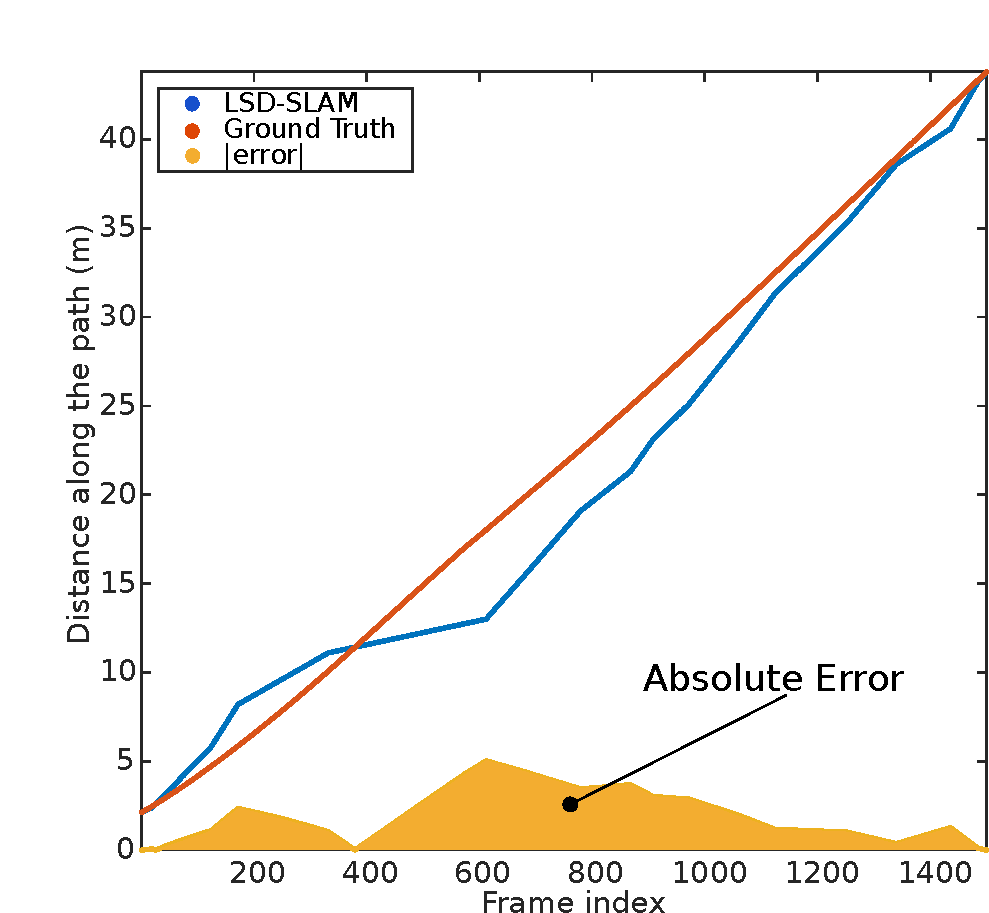
\includegraphics[width=0.45\textwidth]{./gfx/Chapter04/lsd_slam_normal.pdf}\label{fig:slamperfB}
	}
	\caption{Localisation performance in LSD-SLAM; this shows that in different corridors, the accuracy of LSD-SLAM can change quite significantly. See text for details of the SLAM parameters and the nature of the dataset, but note that these were obtained at an image resolution of $1024 \times 576$ pixels. At lower resolutions, loss of tracking dominated the experiments. The difference in the $x$ and $y$ axis labelling is because experiments in a) and b) are obtained from two different corridors with different lengths and different number of frames.}
	\label{fig:slamperf}
\end{figure}


\subsubsection{CDF comparisons}

CDFs, as introduced in Section \ref{sec:CDFs} illustrate very well the differences in the performance of methods. As we can see from Figure \ref{fig:cdf} the appearance-based method using Gabor-based descriptors performs better than LSD-SLAM in the RSM dataset. 

\begin{figure}
\centering
%\setlength\figureheight{0.6\textwidth}
%\setlength\figurewidth{0.8\textwidth}
%% This file was created by matlab2tikz.
% Minimal pgfplots version: 1.3
%
%The latest updates can be retrieved from
%  http://www.mathworks.com/matlabcentral/fileexchange/22022-matlab2tikz
%where you can also make suggestions and rate matlab2tikz.
%
\definecolor{mycolor1}{rgb}{0.85098,0.32549,0.09804}%
\definecolor{mycolor2}{rgb}{0.00000,0.44706,0.74118}%

%
\begin{tikzpicture}

\begin{axis}[%
width=0.95092\figurewidth,
height=\figureheight,
at={(0\figurewidth,0\figureheight)},
scale only axis,
xmin=0,
xmax=100,
xtick={0,10,20,30,40,50,60,70,80,90,100},
xticklabels={{0},{},{},{},{},{25},{},{},{},{},{50}},
xlabel={x (location error in m)},
ymin=0,
ymax=1,
ylabel={$\text{P(}|\epsilon|\text{ \textless x)}$},
legend style={at={(0.659432,0.743536)},anchor=south west,legend cell align=left,align=left,draw=white!15!black}
]

\addplot[area legend,fill=mycolor1,opacity=3.000000e-01,draw=mycolor1,opacity=1]
table[row sep=crcr] {%
x	y\\
0	0.0698\\
1	0.1626\\
2	0.2411\\
3	0.3069\\
4	0.3698\\
5	0.4262\\
6	0.4851\\
7	0.527\\
8	0.5673\\
9	0.6134\\
10	0.673\\
11	0.7104\\
12	0.7412\\
13	0.7789\\
14	0.8016\\
15	0.815\\
16	0.8264\\
17	0.8376\\
18	0.8516\\
19	0.8619\\
20	0.8724\\
21	0.8817\\
22	0.8911\\
23	0.8983\\
24	0.9123\\
25	0.9244\\
26	0.9324\\
27	0.9398\\
28	0.9487\\
29	0.9577\\
30	0.9649\\
31	0.9719\\
32	0.9753\\
33	0.9812\\
34	0.9861\\
35	0.9893\\
36	0.9905\\
37	0.9918\\
38	0.9937\\
39	0.9949\\
40	0.9951\\
41	0.9956\\
42	0.9962\\
43	0.9966\\
44	0.9967\\
45	0.9969\\
46	0.9973\\
47	0.9974\\
48	0.9974\\
49	0.9976\\
50	0.9978\\
51	0.9979\\
52	0.9979\\
53	0.9982\\
54	0.9983\\
55	0.998599999999999\\
56	0.998599999999999\\
57	0.9986\\
58	0.9989\\
59	0.999\\
60	0.9992\\
61	0.9993\\
62	0.9994\\
63	0.999699999999999\\
64	0.999899999999999\\
65	0.999999999999999\\
66	1\\
67	1\\
68	1\\
69	1\\
70	1\\
71	1\\
72	1\\
73	1\\
74	1\\
75	1\\
76	1\\
77	1\\
78	1\\
79	1\\
80	1\\
81	1\\
82	1\\
83	1\\
84	1\\
85	1\\
86	1\\
87	1\\
88	1\\
89	1\\
90	1\\
91	1\\
92	1\\
93	1\\
94	1\\
95	1\\
96	1\\
97	1\\
98	1\\
99	1\\
99	0.999999999999999\\
98	0.999999999999999\\
97	0.999999999999999\\
96	0.999999999999999\\
95	0.999999999999999\\
94	0.999999999999999\\
93	0.999999999999999\\
92	0.999999999999999\\
91	0.999999999999999\\
90	0.999999999999999\\
89	0.999999999999999\\
88	0.999999999999999\\
87	0.999999999999999\\
86	0.999999999999999\\
85	0.999999999999999\\
84	0.999999999999999\\
83	0.999999999999999\\
82	0.999999999999999\\
81	0.999999999999999\\
80	0.999999999999999\\
79	0.999999999999999\\
78	0.999999999999999\\
77	0.999999999999999\\
76	0.999999999999999\\
75	0.999999999999999\\
74	0.999999999999999\\
73	0.999999999999999\\
72	0.999999999999999\\
71	0.999999999999999\\
70	0.999999999999999\\
69	0.999999999999999\\
68	0.999999999999999\\
67	0.999999999999999\\
66	0.998199999999999\\
65	0.997599999999999\\
64	0.997099999999999\\
63	0.996899999999999\\
62	0.996399999999999\\
61	0.996299999999999\\
60	0.995999999999999\\
59	0.995899999999999\\
58	0.995499999999999\\
57	0.9952\\
56	0.995\\
55	0.994899999999999\\
54	0.994799999999999\\
53	0.994599999999999\\
52	0.994199999999999\\
51	0.993799999999999\\
50	0.993599999999999\\
49	0.9934\\
48	0.993\\
47	0.993\\
46	0.9926\\
45	0.9926\\
44	0.9924\\
43	0.9921\\
42	0.9918\\
41	0.9911\\
40	0.9906\\
39	0.99\\
38	0.9872\\
37	0.9847\\
36	0.9833\\
35	0.9821\\
34	0.9783\\
33	0.9721\\
32	0.9659\\
31	0.962\\
30	0.9531\\
29	0.9447\\
28	0.9349\\
27	0.9253\\
26	0.9156\\
25	0.906\\
24	0.8944\\
23	0.8804\\
22	0.8706\\
21	0.8606\\
20	0.8499\\
19	0.8379\\
18	0.8258\\
17	0.8139\\
16	0.8013\\
15	0.7878\\
14	0.7742\\
13	0.7496\\
12	0.7109\\
11	0.6784\\
10	0.6409\\
9	0.5833\\
8	0.5377\\
7	0.4988\\
6	0.4554\\
5	0.3985\\
4	0.3431\\
3	0.2811\\
2	0.2135\\
1	0.1408\\
0	0.0521\\
}--cycle;

\addlegendentry{SF-GABOR};


\addplot[area legend,solid,line width=2.0pt,fill=mycolor2,opacity=1,draw=mycolor2]
table[row sep=crcr] {%
x	y\\
0	0.2518\\
1	0.5535\\
2	0.6908\\
3	0.7428\\
4	0.8196\\
5	0.8631\\
6	0.904\\
7	0.938\\
8	0.9486\\
9	0.9661\\
10	0.9756\\
11	0.9859\\
12	0.9882\\
13	0.9905\\
14	0.9918\\
15	0.9931\\
16	0.9937\\
17	0.9946\\
18	0.9951\\
19	0.9952\\
20	0.9952\\
21	0.9955\\
22	0.9955\\
23	0.9955\\
24	0.9959\\
25	0.9962\\
26	0.9962\\
27	0.9963\\
28	0.9964\\
29	0.9965\\
30	0.9965\\
31	0.9965\\
32	0.9966\\
33	0.997\\
34	0.9971\\
35	0.9974\\
36	0.9977\\
37	0.9977\\
38	0.9977\\
39	0.9977\\
40	0.9977\\
41	0.9977\\
42	0.9977\\
43	0.9977\\
44	0.9977\\
45	0.9978\\
46	0.9978\\
47	0.997899999999999\\
48	0.997899999999999\\
49	0.997899999999999\\
50	0.9979\\
51	0.9979\\
52	0.998\\
53	0.998299999999999\\
54	0.998399999999999\\
55	0.998399999999999\\
56	0.998399999999999\\
57	0.998499999999999\\
58	0.998699999999999\\
59	0.998799999999999\\
60	0.998999999999999\\
61	0.998999999999999\\
62	0.999099999999999\\
63	0.999099999999999\\
64	0.999199999999999\\
65	0.999199999999999\\
66	0.999199999999999\\
67	0.999299999999999\\
68	0.999299999999999\\
69	0.999499999999999\\
70	0.999699999999999\\
71	0.999699999999999\\
72	0.999799999999999\\
73	0.999799999999999\\
74	0.999799999999999\\
75	0.999799999999999\\
76	0.999799999999999\\
77	0.999799999999999\\
78	0.999799999999999\\
79	0.999799999999999\\
80	0.999899999999999\\
81	0.999899999999999\\
82	0.999999999999999\\
83	0.999999999999999\\
84	0.999999999999999\\
85	1\\
86	1\\
87	1\\
88	1\\
89	1\\
90	1\\
91	1\\
92	1\\
93	1\\
94	1\\
95	1\\
96	1\\
97	1\\
98	1\\
99	1\\
99	0.999999999999999\\
98	0.999999999999999\\
97	0.999999999999999\\
96	0.999999999999999\\
95	0.999999999999999\\
94	0.999999999999999\\
93	0.999799999999999\\
92	0.999799999999999\\
91	0.999799999999999\\
90	0.999799999999999\\
89	0.999699999999999\\
88	0.999499999999999\\
87	0.999499999999999\\
86	0.999299999999999\\
85	0.999299999999999\\
84	0.998799999999999\\
83	0.998199999999999\\
82	0.998099999999999\\
81	0.997699999999999\\
80	0.997599999999999\\
79	0.997399999999999\\
78	0.997299999999999\\
77	0.997299999999999\\
76	0.997199999999999\\
75	0.997199999999999\\
74	0.997099999999999\\
73	0.996899999999999\\
72	0.996899999999999\\
71	0.996799999999999\\
70	0.996799999999999\\
69	0.996699999999999\\
68	0.996499999999999\\
67	0.996399999999999\\
66	0.996399999999999\\
65	0.996199999999999\\
64	0.995999999999999\\
63	0.995999999999999\\
62	0.995999999999999\\
61	0.995999999999999\\
60	0.995999999999999\\
59	0.995999999999999\\
58	0.995899999999999\\
57	0.9954\\
56	0.9952\\
55	0.9949\\
54	0.9949\\
53	0.9946\\
52	0.9943\\
51	0.994\\
50	0.994\\
49	0.9939\\
48	0.9939\\
47	0.9939\\
46	0.9939\\
45	0.9939\\
44	0.9936\\
43	0.9935\\
42	0.9934\\
41	0.9934\\
40	0.9934\\
39	0.9934\\
38	0.9934\\
37	0.9934\\
36	0.9932\\
35	0.9932\\
34	0.9928\\
33	0.9926\\
32	0.9921\\
31	0.9918\\
30	0.9916\\
29	0.9913\\
28	0.9913\\
27	0.9913\\
26	0.9913\\
25	0.9913\\
24	0.9911\\
23	0.9908\\
22	0.9908\\
21	0.9906\\
20	0.9906\\
19	0.9903\\
18	0.9901\\
17	0.9896\\
16	0.9886\\
15	0.9876\\
14	0.9858\\
13	0.9835\\
12	0.9809\\
11	0.9784\\
10	0.965\\
9	0.9536\\
8	0.9346\\
7	0.9213\\
6	0.8836\\
5	0.8376\\
4	0.7898\\
3	0.7125\\
2	0.6578\\
1	0.517\\
0	0.2218\\
}--cycle;

\addlegendentry{LSD-SLAM};

\end{axis}
\end{tikzpicture}% %
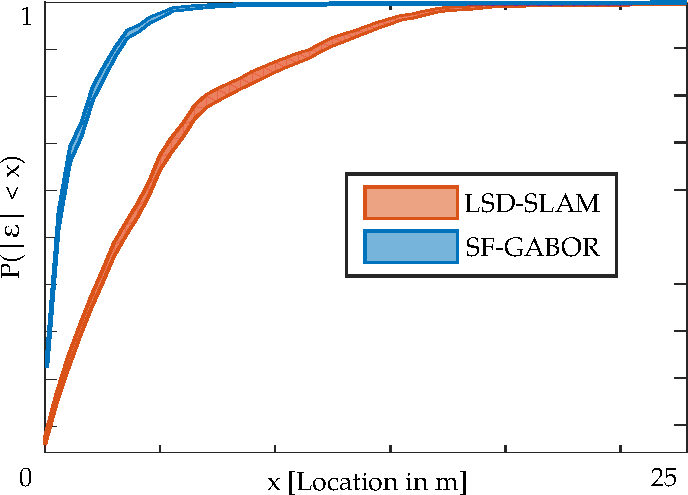
\includegraphics[width=0.8\textwidth]{gfx/Chapter04/SF_GABORvsLSD_SLAM.pdf}
\caption{CDF of SF-GABOR and LSD-SLAM when sampling 10 million random queries from all the error measurements. The width of the curves represent the variability of the result data. The bounds are the maximum and minimum CDF values obtained from the Monte-Carlo sampling.}
\label{fig:cdf}
\end{figure}

Another perspective to these results can be seen from Table~\ref{tbl:cdftable}, where we can see a head to head comparison for the probabilities of achieving a localisation error smaller than $x$ in metres. We can see how SF-GABOR achieves smaller localisation errors than LSD-SLAM with a larger probability. For the sample of CDF values obtained, we can see that SF-GABOR can localise with an error below 2.5 m in the 95.95\% of the times, whilst LSD-SLAM can only guarantee errors below 2.5 m 59.88\% of the times on average.

This does not imply that the appearance-based technique used should \textit{replace} SLAM or its equivalents -- it is merely a different context of usage. A user who is interested in getting from $A$ to $B$ may be less interested in mapping the geometry along that route than whether their trajectory matches that of other users who have previously made the same journey. In the scenario described, and in which performance is being compared, the journey of a user is assessed against those made by other people who have made the same journey -- location becomes journey-relative, not map-relative. The usage scenario also means that loop closure may not be possible. However, localisation systems may aim for a combined solution, as LSD-SLAM seems to perform better given an appearance-based loop closure method \citep{engel14eccv} such as FabMap, which could be replaced by any of the solutions proposed \citep{Rivera-Rubio2015PRL} or a combination of both.

%A final point to remember is that the cameras that are used in capturing the journeys are not necessarily identical, and certainly may be uncalibrated.

\begin{table}
\centering
    \begin{tabular}{lcccc}
    %\begin{tabular}{lSSSSSS}
    \toprule
    %\hline
    Method & 
    \multicolumn{2}{c}{SF-GABOR} &
    \multicolumn{2}{c}{LSD-SLAM} \\

    $x$ (m) & Ave. $P$  & (min $P$, max $P$ ) & Ave. $P$ & (min $P$, max $P$) \\
    \midrule
    0.25 & 0.23 & (0.22, 0.25) & 0.06 & (0.05, 0.07)  \\
    0.50 & 0.53 & (0.52, 0.55) & 0.15 & (0.14, 0.16) \\
    0.75 & 0.67 & (0.66, 0.69) & 0.23 & (0.21, 0.24) \\
    1.00 & 0.73 & (0.71, 0.74) & 0.29 & (0.28, 0.31)\\
    1.25 & 0.80 & (0.79, 0.82) & 0.36 & (0.34, 0.37)\\
    1.50 & 0.85 & (0.84, 0.86) & 0.41 & (0.40, 0.42) \\
    1.75 & 0.89 & (0.88, 0.90) & 0.47 & (0.46, 0.49) \\
    2.00 & 0.92 & (0.92, 0.94) & 0.51 & (0.50, 0.53)  \\
    2.25 & 0.94 & (0.93, 0.95) & 0.55 & (0.54, 0.57) \\
    2.50 & 0.96 & (0.95, 0.97)  & 0.60 & (0.58, 0.61) \\
    \bottomrule
    \end{tabular}
    \caption{Cumulative distribution function values against localisation error in metres ($\epsilon$). $P(|\epsilon| \leq x)$, expressed as a percentage. From this table, the best appearance-based method achieves a probability of 90\% of localising with an error below $2$ m, whilst LSD-SLAM achieves just above 50\% accuracy level for that error boundary, and required images 5 times larger. In addition, the performance of LSD-SLAM was significantly worse (compare the minimum performance colums) on some corridors and journeys, bringing the overall average down across the RSM dataset relative to appearance-based localisation.}
\label{tbl:cdftable}
\end{table}


\subsubsection{Reproducibility errors}

Another comparison is illustrated by Figure \ref{fig:reprod}. These box-and-whisker plots evaluate the comparative reproducibility in localisation between the best appearance-based method, SF-GABOR, and LSD-SLAM within RSM corridors 1 and 3 (C1 and C3) for multiple ``leave-one-out'' passes. The plots suggest that whilst LSD-SLAM yielded worse results in terms of error, it has a consistency in performance that is comparable to that of SF-GABOR. Also, the errors for LSD-SLAM rarely go beyond $5$ m, with an average of $\mu_e = 2.48 \pm 2.37$ m. Conversely, the appearance-based method contains some outliers; even so, for some sequences the error is of the same order of magnitude or lower ($\mu_e = 1.59 \pm 0.11$ m) than the best reported for SLAM, supporting the idea of an appearance-based localisation approach for indoor navigation. 

\begin{figure}
\centering
\subfloat[C1 SF-GABOR]{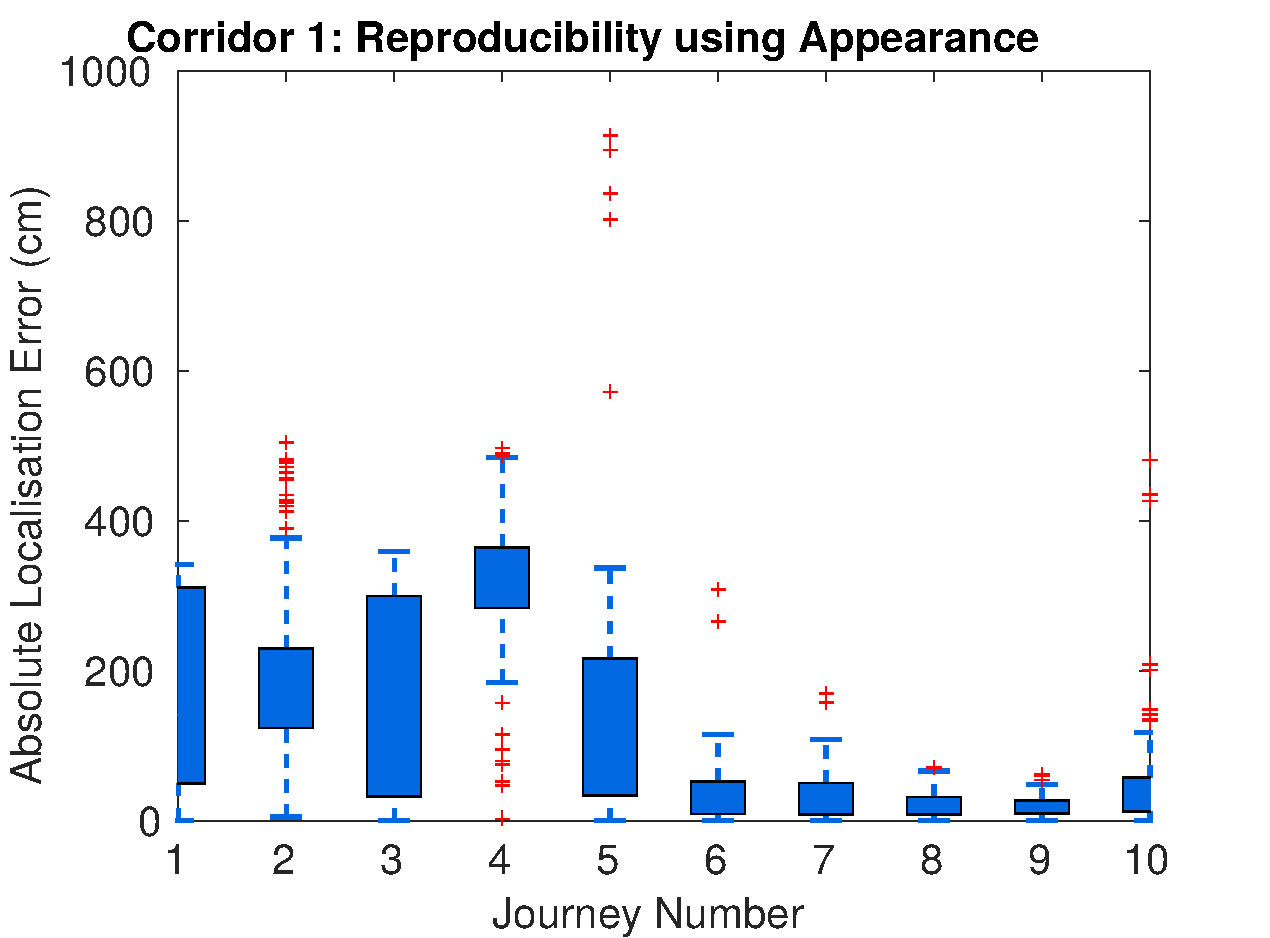
\includegraphics[width=0.5\linewidth]{./gfx/Chapter04/Corr1RepApp.pdf}}
\subfloat[C3 SF-GABOR]{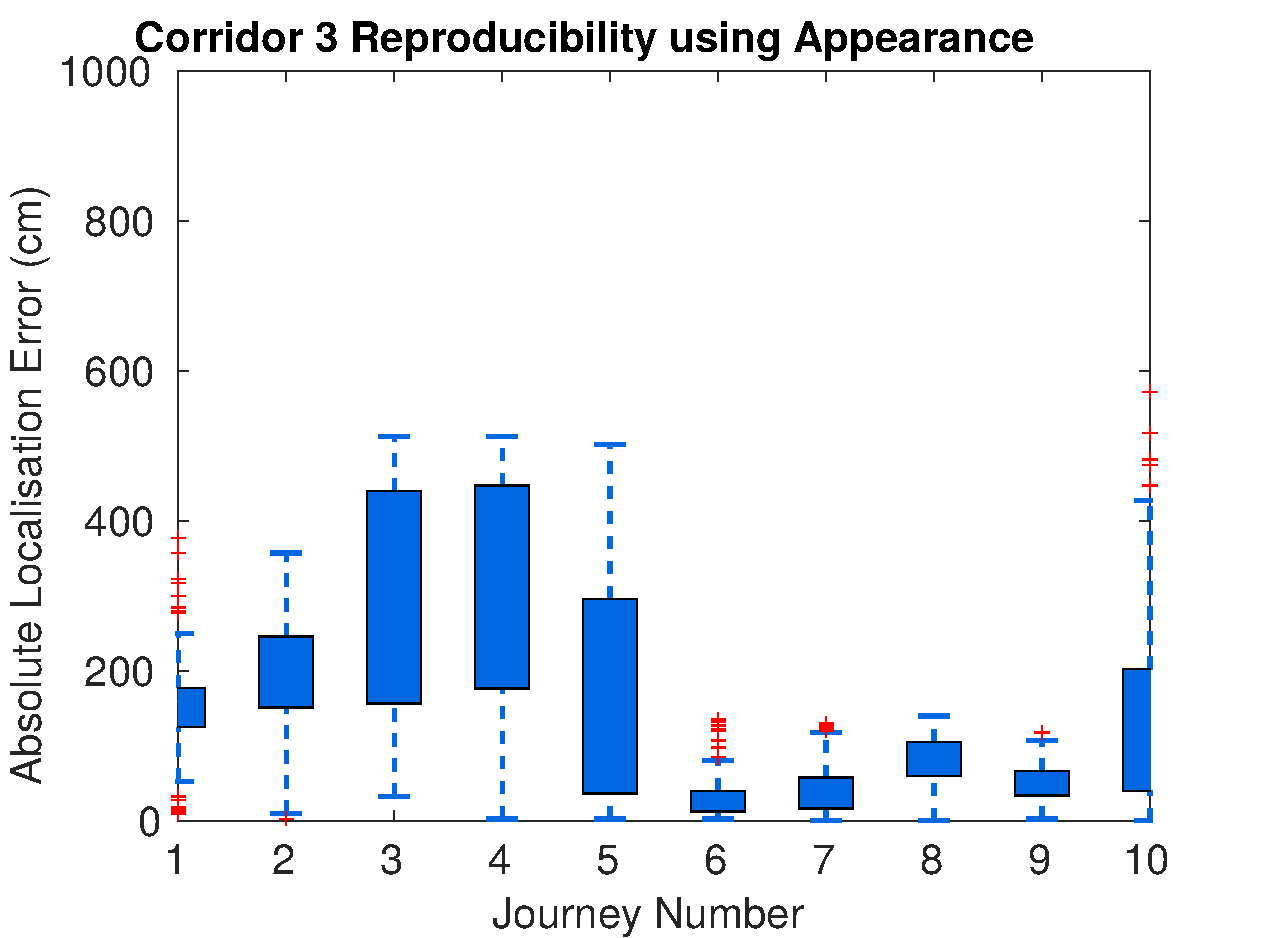
\includegraphics[width=0.5\linewidth]{./gfx/Chapter04/Corr3RepApp.pdf}}


\subfloat[C1 LSD-SLAM]{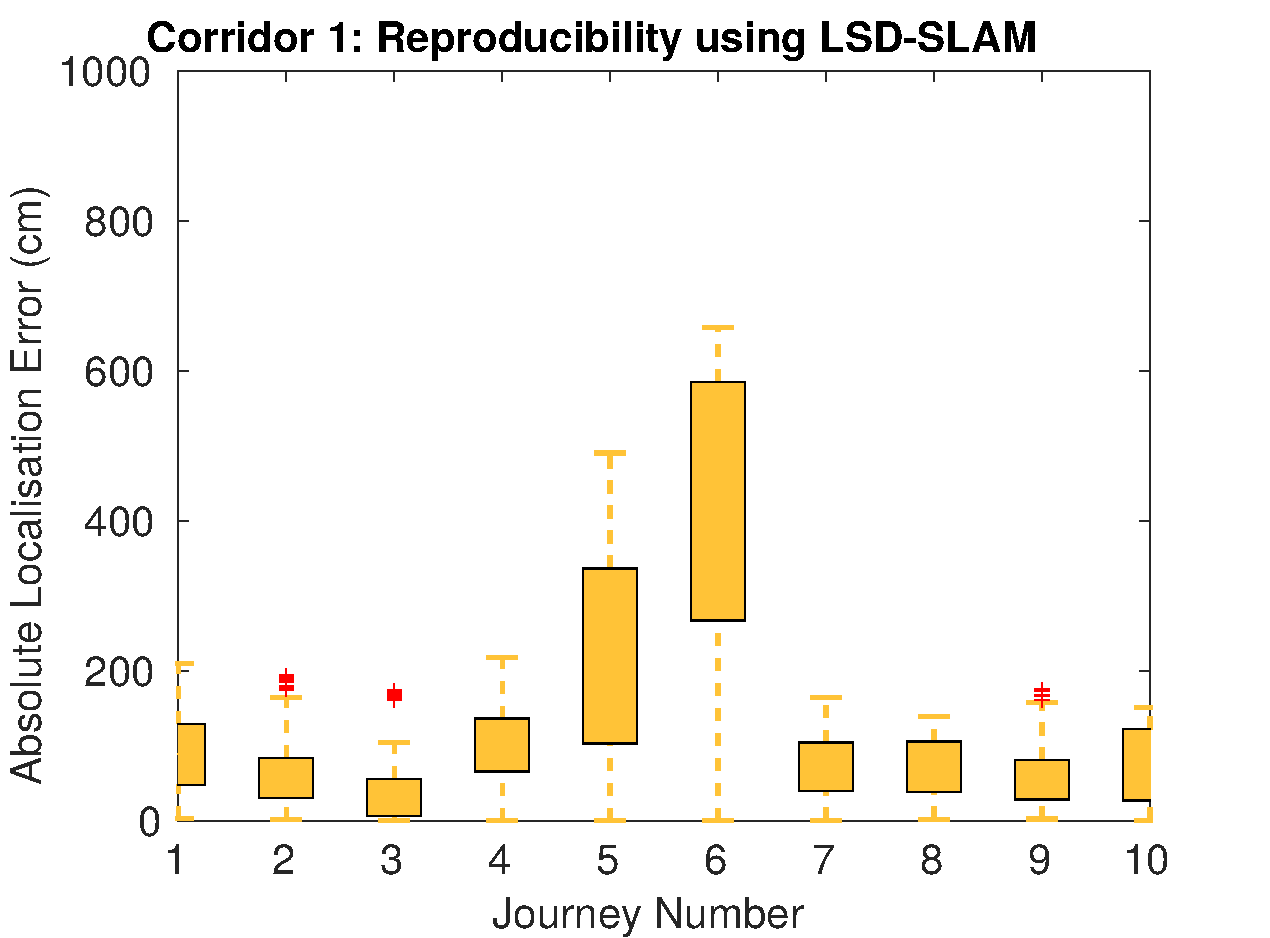
\includegraphics[width=0.5\linewidth]{./gfx/Chapter04/Corr1RepSLAM.pdf}}
\subfloat[C3 LSD-SLAM]{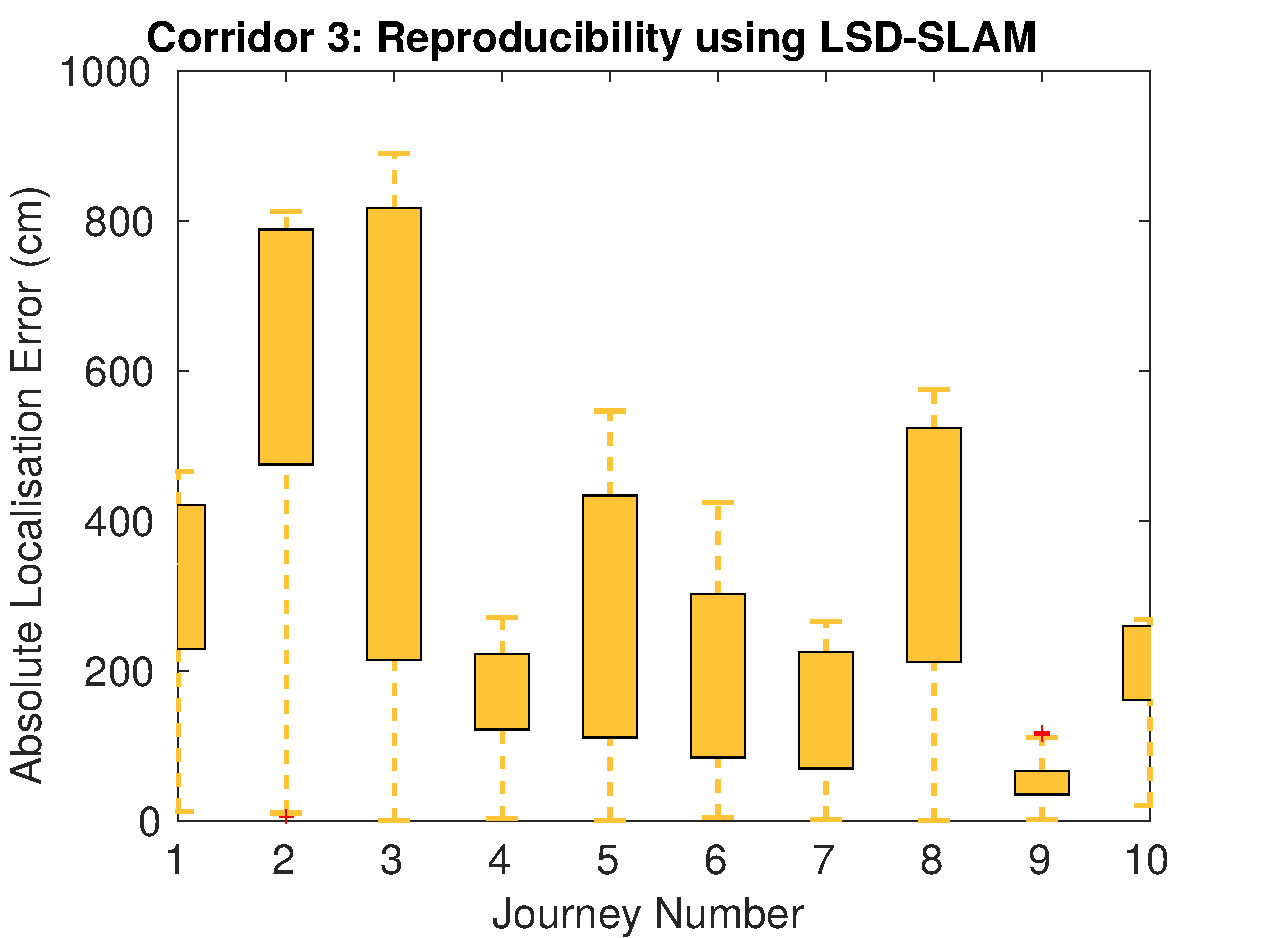
\includegraphics[width=0.5\linewidth]{./gfx/Chapter04/Corr3RepSLAM.pdf}}

\caption{Box-and-whisker plots depicting the errors obtained in two corridors, using either LSD-SLAM or appearance-based matching using SF-GABOR descriptors. The top row corresponds to the appearance-based result. The bottom row corresponds to LSD-SLAM. On each graph, the horizontal positions correspond to different journeys down the same corridor when the remainder of journeys is used as a database of journeys. Each of these positions represents the statistics of 100 random image queries. These graphs suggest that LSD-SLAM and an appearance-based approach are comparable in terms of reproducibility of localisation within the same corridor. Note, however, that much lower spatial resolution (less than 1/4 of the image size) is used for the appearance-based technique than for LSD-SLAM.}
\label{fig:reprod}
\end{figure}

\subsubsection{Area-Under-Curve comparisons}
In Section \ref{visloc_perf} I calculated the average absolute positional error (in m) and the standard deviation of the absolute positional errors for a variety of methods. Here, I reproduce the AUC results for the method SF-GABOR, which ranged from 96.11\% to 96.39\%. For the case of LSD-SLAM, the AUC ranged from 89.71\% to 90.61\% All queries were again performed by adopting the leave-one-out strategy, but because of the high repeatability of results, random frame-level sampling was not applied.  



%------------------------------------------------------------------------- 
\section{A visualisation of the frame distribution with t-SNE}

In the previous sections I have extensively studied the case of the localisation within a journey, answering the question ``where am I along the path?'' that was introduced in Chapter \ref{ch:chapter2}. In a visual path retrieval system divided in different journeys inside a building, to be able to answer the question ``in which path am I on?'' with precision would give this system the necessary prior information to provide a better location and also suggest path planning, which would be specially relevant in an assistive context as we will see in Chapter \ref{ch:chapter6}. Although the journey selection was beyond the scope of this thesis, it was informative to study the behaviour of a state-of-the-art dimensionality reduction technique in a rather challenging scenario of having such highly dimensional data (the BOVW-encoded vectors have 4,000 elements). Therefore I chose t-SNE as a technique for visualising in two or three dimensions the high dimensional descriptor space of the RSM dataset.

t-distributed stochastic neighbour embedding (t-SNE) is a machine learning algorithm for dimensionality reduction developed by Laurens van der Maaten and Geoffrey Hinton \cite{maaten2009learning}. It is a non-linear dimensionality reduction technique that is particularly well suited for embedding high-dimensional data into a space of two or three dimensions, which can then be visualised in a scatter plot. Specifically, it models each high-dimensional object by a two- or three-dimensional point in such a way that similar objects are modelled by nearby points and dissimilar objects are modelled by distant points.

In other words, t-SNE is a dimensionality reduction technique that aims to preserve the local structure of the data. For this reason I wanted to compute the visual path descriptions of the RSM dataset and build the foundations for future work on journey/corridor selection.

\begin{figure}
\centering
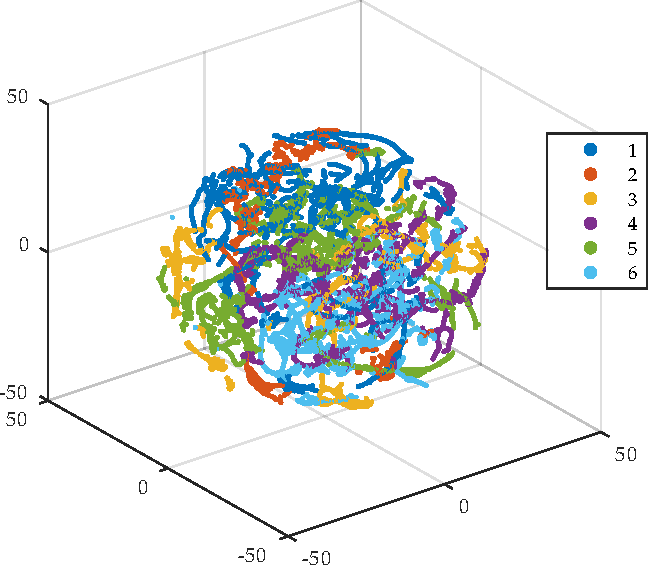
\includegraphics[width=\textwidth]{gfx/Chapter04/tsne_dsift_3d.pdf}
\caption{Distribution of the BOVW data of the RSM dataset in a reduced 3D space when visualised with t-SNE. Colours refer to different corridors in the dataset. Note that there is some evidence of the locally connected paths in the visual-words space.}
\label{fig:tsne3d}
\end{figure}

In Figure \ref{fig:tsne3d} we can see the 4,000-dimension visual word reduced to three dimensions and in Figure \ref{fig:tsne2d} we can see the two-dimensional embedding. The embeddings were generated using more than 50,000 randomly selected examples from all the corridors. Following the method described in Section~\ref{sec:quant_and_encod}, I selected for this particular example dense-SIFT descriptors encoded with hard assignment (HA), using $k$-means to create the visual word examples.

As we can see from the images, the difficulty of generating two or three-dimensional embeddings of such a high dimensional and complex dataset is notable. However, patterns showing how examples from the same corridors can display a sequential relationship within the embeddings.


\begin{figure}
\centering
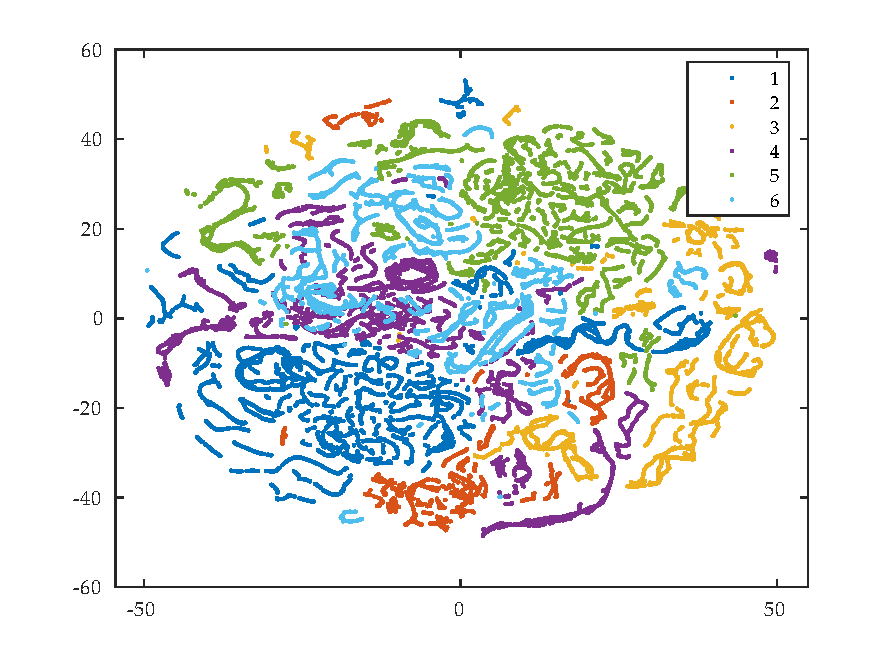
\includegraphics[width=\textwidth]{gfx/Chapter04/tsne_dsift_2d.pdf}
\caption{Distribution of the BOW data of the RSM dataset in a reduced 2D space when visualised with t-SNE. It is easy to identify some sets of points that form locally one-dimensional structures. Though they are not always contiguous for one corridor, the concept of visual paths appears at least partially justified.}
\label{fig:tsne2d}
\end{figure}

The present thesis gives an emphasis on understanding \textit{visual path} data from a journey perspective, from a crowdsourced collection of journeys in particular. However, although of limited practical use within journey localisation, this visualisation is the first step in understanding the structure of the data from a ``building'' perspective.

It is therefore subject of future work the use of these visualisations to understand the important features of visual paths datasets such as the presence of global clusters that reveal remarkable distinctiveness between journeys or give insight on how to optimise the retrieval based on between-journey differences.

%------------------------------------------------------------------------- 
\section{Conclusion}

I have presented three main contributions to the topic of indoor localisation using visual path matching from wearable and hand-held cameras. In first place, a complete evaluation of six local descriptor methods is provided: three custom designed and three standard image (KP-SIFT and DSIFT) and video (HOG3D) matching methods as baseline. These local descriptions follow a standard bag-of-words and kernel encoding pipeline. The code for both the local descriptors and for the evaluation pipeline is available online~\cite{jose_rivera_rubio_2015_33762}. In second place, the RSM dataset is also made available, a large dataset of more than 90,000 video frames with positional ground truth of indoor journeys to complete the evaluation framework. The dataset is freely available at \url{http://rsm.bicv.org}. In third place, I introduce the CDFs of the error as the probability of the error being less than a certain threshold. This way of reporting localisation errors is a different performance metric than the usual average error with respect to the ground truth (although this is also provided) found in SLAM and other localisation approaches.

The results show that there is significant localisation information in the visual data, and that errors as small as \SI{1.5}{m} over a \SI{50}{m} distance can be achieved, even without tracking. As mentioned above, the results have been reported in two ways: a) average absolute positional errors, and b) error distributions, both of which allow image descriptions to be assessed for their localisation capability.  The latter could also be used to build a measurement model for inclusion in a Kalman or particle filter  aimed at supporting human ambulatory navigation. 

As a baseline for these results, I provide a comparison with the state of the art method in SLAM, LSD-SLAM, with the best appearance-based method, SF-GABOR. It was found, rather surprisingly, that appearance-based localisation appeared to be at least as accurate as that of LSD-SLAM without loop closure over a distance of around 50 m. In particular, SF-GABOR presents a lower average localisation error ($\mu_{e,SF-GABOR} = 1.59 $ m $< \mu_{e,LSD-SLAM} = 2.48 $ m). It was also found that a\-ppea\-rance\--based localisation was achievable with low resolution images, of around 30,000 pixels per image -- a 5\% of the number of pixels in the frames used for the LSD-SLAM experiment. This lowers the computational burden, a potentially important factor in an assistive context where device power autonomy can hinder the use of power-hungry computer vision algorithms. In addition, the small file sizes required for the appearance-based localisation approach reduces the bandwidth and storage required for crowdsourcing data. Results show that 1,500-frame sequences, sufficient for a 50 m corridor at normal walking speeds, consumed no more than 2 MB once compressed, meaning that the journey segments required can feasibly be crowdsourced from several users within a building.

Finally, the high-dimensional visual word space representing the RSM dataset is visualised in 2D and 3D using t-SNE, a powerful dimensionality reduction algorithm for visualisations. The aim of this visualisation is to lay the foundations for future studies on retrieval at the building or large scale level, rather than at the journey level as in this thesis.

We plan to introduce tracking in future work. There are, of course, numerous other enhancements that one could make for a system that uses visual data; integration of data from other sensors springs to mind, such as inertial sensing, magnetometers and RSSI.  Although fusing independent and informative data sources would theoretically lead to improvements in performance, we would argue that the methods applied to infer location from each information source should be rigorously tested, both in isolation and as part of an integrated system.  This would help ensure that real-world systems would be somewhat robust to sensor failure. We anticipate that using vision to associate locations in the journeys of several users through their visual paths could play an important role in navigation. In fact, in the next chapter I delve deeper into the importance of appearance-based retrieval techniques in localisation and explore the similarities of these techniques with those present in biology. I develop a model of biological mimicry to configure a localisation system inspired in biological place cells found in mammals.


\label{sec:conclusion}


%*****************************************
%*****************************************
%*****************************************
%*****************************************
%*****************************************
